\mysection{Measurements related to Unitarity Triangle angles
}
\label{sec:cp_uta}

The charge of the ``$\CP(t)$ and Unitarity Triangle angles'' group
is to provide averages of measurements 
from time-dependent asymmetry analyses,
and other quantities that are related 
to the angles of the Unitarity Triangle (UT).
In cases where considerable theoretical input is required to 
extract the fundamental quantities, no attempt is made to do so at 
this stage. However, straightforward interpretations of the averages 
are given, where possible.

In Sec.~\ref{sec:cp_uta:introduction} 
a brief introduction to the relevant phenomenology is given.
In Sec.~\ref{sec:cp_uta:notations}
an attempt is made to clarify the various different notations in use.
In Sec.~\ref{sec:cp_uta:common_inputs}
the common inputs to which experimental results are rescaled in the
averaging procedure are listed. 
We also briefly introduce the treatment of experimental errors. 
In the remainder of this section,
the experimental results and their averages are given,
divided into subsections based on the underlying quark-level decays.

\mysubsection{Introduction
}
\label{sec:cp_uta:introduction}

The Standard Model Cabibbo-Kobayashi-Maskawa (CKM) quark mixing matrix $\VCKM$ 
must be unitary. A $3 \times 3$ unitary matrix has four free parameters,\footnote{
  In the general case there are nine free parameters,
  but five of these are absorbed into unobservable quark phases.}
and these are conventionally written by the product
of three (complex) rotation matrices~\cite{Chau:1984fp}, 
where the rotations are characterised by the Euler angles 
$\theta_{12}$, $\theta_{13}$ and $\theta_{23}$, which are the mixing angles
between the generations, and one overall phase $\delta$,
\begin{equation}
\label{eq:ckmPdg}
\VCKM =
        \left(
          \begin{array}{ccc}
            V_{ud} & V_{us} & V_{ub} \\
            V_{cd} & V_{cs} & V_{cb} \\
            V_{td} & V_{ts} & V_{tb} \\
          \end{array}
        \right)
        =
        \left(
        \begin{array}{ccc}
        c_{12}c_{13}    
                &    s_{12}c_{13}   
                        &   s_{13}e^{-i\delta}  \\
        -s_{12}c_{23}-c_{12}s_{23}s_{13}e^{i\delta} 
                &  c_{12}c_{23}-s_{12}s_{23}s_{13}e^{i\delta} 
                        & s_{23}c_{13} \\
        s_{12}s_{23}-c_{12}c_{23}s_{13}e^{i\delta}  
                &  -c_{12}s_{23}-s_{12}c_{23}s_{13}e^{i\delta} 
                        & c_{23}c_{13} 
        \end{array}
        \right)
\end{equation}
where $c_{ij}=\cos\theta_{ij}$, $s_{ij}=\sin\theta_{ij}$ for 
$i<j=1,2,3$. 

Following the observation of a hierarchy between the different
matrix elements, the Wolfenstein parametrisation~\cite{Wolfenstein:1983yz}
is an expansion of $\VCKM$ in terms of the four real parameters $\lambda$
(the expansion parameter), $A$, $\rho$ and $\eta$. Defining to 
all orders in $\lambda$~\cite{Buras:1994ec}
\begin{eqnarray}
  \label{eq:burasdef}
  s_{12}             &\equiv& \lambda\,,\nonumber \\ 
  s_{23}             &\equiv& A\lambda^2\,, \\
  s_{13}e^{-i\delta} &\equiv& A\lambda^3(\rho -i\eta)\,,\nonumber
\end{eqnarray}
and inserting these into the representation of Eq.~(\ref{eq:ckmPdg}), 
unitarity of the CKM matrix is achieved to all orders.
A Taylor expansion of $\VCKM$ leads to the familiar approximation
\begin{equation}
  \label{eq:cp_uta:ckm}
  \VCKM
  = 
  \left(
    \begin{array}{ccc}
      1 - \lambda^2/2 & \lambda & A \lambda^3 ( \rho - i \eta ) \\
      - \lambda & 1 - \lambda^2/2 & A \lambda^2 \\
      A \lambda^3 ( 1 - \rho - i \eta ) & - A \lambda^2 & 1 \\
    \end{array}
  \right) + {\cal O}\left( \lambda^4 \right) \, .
\end{equation}
At order $\lambda^{5}$, the obtained CKM matrix in this extended
Wolfenstein parametrisation is:
{\small
  \begin{equation}
    \label{eq:cp_uta:ckm_lambda5}
    \VCKM
    =
    \left(
      \begin{array}{ccc}
        1 - \frac{1}{2}\lambda^{2} - \frac{1}{8}\lambda^4 &
        \lambda &
        A \lambda^{3} (\rho - i \eta) \\
        - \lambda + \frac{1}{2} A^2 \lambda^5 \left[ 1 - 2 (\rho + i \eta) \right] &
        1 - \frac{1}{2}\lambda^{2} - \frac{1}{8}\lambda^4 (1+4A^2) &
        A \lambda^{2} \\
        A \lambda^{3} \left[ 1 - (1-\frac{1}{2}\lambda^2)(\rho + i \eta) \right] &
%        -A \lambda^{2}(1-\frac{1}{2}\lambda^2) \left[ 1 + \lambda^{2}(\rho + i \eta) \right] &
        -A \lambda^{2} + \frac{1}{2}A\lambda^4 \left[ 1 - 2(\rho + i \eta) \right] &
        1 - \frac{1}{2}A^2 \lambda^4
      \end{array} 
    \right) + {\cal O}\left( \lambda^{6} \right)\,.
  \end{equation}
}

\vspace{-5mm}
\noindent
The non-zero imaginary part of the CKM matrix,
which is the origin of $\CP$ violation in the Standard Model,
is encapsulated in a non-zero value of $\eta$.

% By definition, the expression for $V_{ub}$ remains unchanged relative
% to the original Wolfenstein parametrization and the
% corrections to $V_{us}$ and $V_{cb}$ appear only at ${\cal O}(\lambda7)$
% and
% ${\cal O}(\lambda8)$, respectively.

%%% TJG this expression for V_{td} is only approximate
%%%     leave it out here and discuss it later
% It can be noted that the element $V_{td}$ can be re-expressed as:
% \begin{equation}
%   V_{td} = A \lambda^{3} (1-\overline{\rho} -i \overline{\eta})
% \end{equation}
% where~\cite{Buras:1994ec}
% \begin{equation}
%   \overline{\rho}=\rho (1-\frac{\lambda^2}{2}) + {\cal O}\left( \lambda^{4} \right),
%   \qquad
%   \overline{\eta}=\eta (1-\frac{\lambda^2}{2}) + {\cal O}\left( \lambda^{4} \right).
% \end{equation}
% This elegant change in $V_{td}$, 
% with respect to the original Wolfenstein parametrization,
% allows a simple generalization of the so-called unitarity triangle to
% higher orders in $\lambda$ as discussed below.

The unitarity relation $\VCKM^\dagger\VCKM = {\mathit 1}$
results in a total of nine expressions,
that can be written as
$\sum_{i=u,c,t} V_{ij}^*V_{ik} = \delta_{jk}$,
where $\delta_{jk}$ is the Kronecker symbol.
Of the off-diagonal expressions ($j \neq k$),
three can be transformed into the other three 
% (under $j \leftrightarrow k$),
leaving six relations, in which three complex numbers sum to zero,
which therefore can be expressed as triangles in the complex plane.
More details about unitarity triangles can be found in Refs.~\cite{Jarlskog:1985ht,Jarlskog:2005uq,Bjorken:2005rm,Harrison:2009bz,Frampton:2010ii,Frampton:2010uq}.

One of these relations,
\begin{equation}
  \label{eq:cp_uta:ut}
  V_{ud}V_{ub}^* + V_{cd}V_{cb}^* + V_{td}V_{tb}^* = 0\,,
\end{equation}
is of particular importance to the $\B$ system, 
being specifically related to flavour changing 
neutral current $b \to d$ transitions.
The three terms in Eq.~(\ref{eq:cp_uta:ut}) are of the same order 
(${\cal O}\left( \lambda^3 \right)$),
and this relation is commonly known as the Unitarity Triangle.
For presentational purposes,
it is convenient to rescale the triangle by $(V_{cd}V_{cb}^*)^{-1}$,
as shown in Fig.~\ref{fig:cp_uta:ut}.

\begin{figure}[t]
  \begin{center}
    \resizebox{0.55\textwidth}{!}{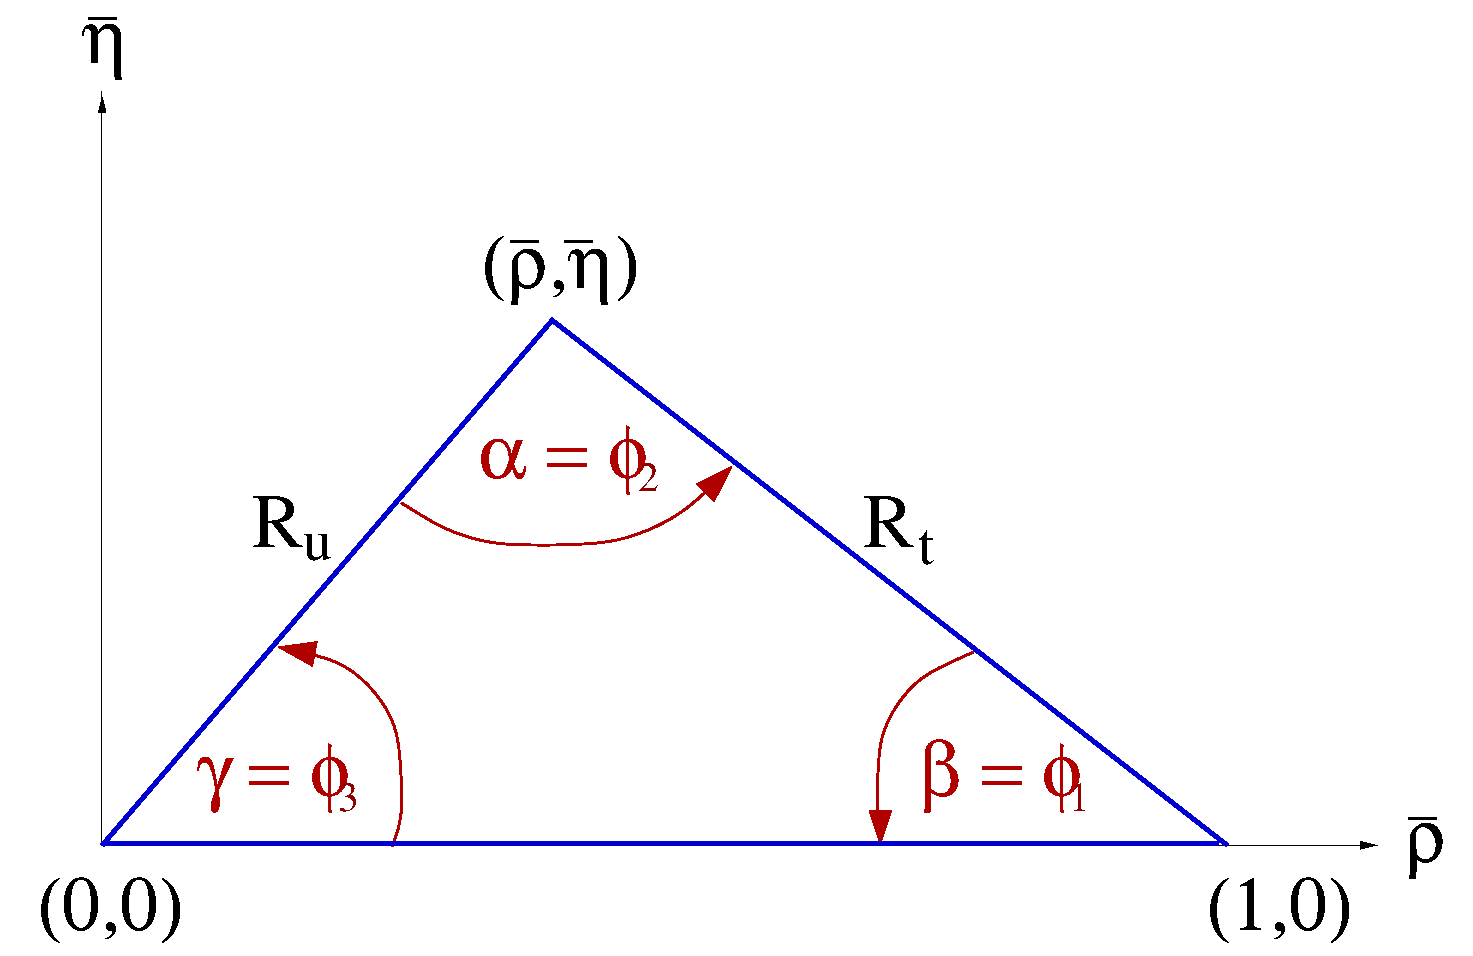
\includegraphics{figures/cp_uta/utriangle_hfag}}
    \caption{The Unitarity Triangle.}
    \label{fig:cp_uta:ut}
  \end{center}
\end{figure}

Two popular naming conventions for the UT angles exist in the literature:
\begin{equation}
  \label{eq:cp_uta:abc}
  \alpha  \equiv  \phi_2  = 
  \arg\left[ - \frac{V_{td}V_{tb}^*}{V_{ud}V_{ub}^*} \right]\,,
  \hspace{0.5cm}
  \beta   \equiv   \phi_1 =  
  \arg\left[ - \frac{V_{cd}V_{cb}^*}{V_{td}V_{tb}^*} \right]\,,
  \hspace{0.5cm}
  \gamma  \equiv   \phi_3  =  
  \arg\left[ - \frac{V_{ud}V_{ub}^*}{V_{cd}V_{cb}^*} \right]\,.
%  \nonumber
\end{equation}
In this document the $\left( \alpha, \beta, \gamma \right)$ set is used.\footnote{
  The relevant unitarity triangle for the $\Bs$ system is obtained 
  by replacing $d \leftrightarrow s$ in Eq.~\ref{eq:cp_uta:ut}.
  Definitions of the set of angles $( \alpha_s, \beta_s, \gamma_s )$ 
  can be obtained using equivalent relations to those of Eq.~\ref{eq:cp_uta:abc},
  for example $\beta_s = \arg\left[ - (V_{cs}V_{cb}^*) / (V_{ts}V_{tb}^*) \right]$.
  This definition gives a value of $\beta_s$ that is negative in the Standard Model,
  so that the sign is often flipped in the literature.
}
The sides $R_u$ and $R_t$ of the Unitarity Triangle 
(the third side being normalised to unity) 
are given by
%% read to all orders 
\begin{equation}
  \label{eq:ru_rt}
  R_u =
  \left|\frac{V_{ud}V_{ub}^*}{V_{cd}V_{cb}^*} \right|
  = \sqrt{\rhobar^2+\etabar^2} \,,
  \hspace{0.5cm}
  R_t = 
  \left|\frac{V_{td}V_{tb}^*}{V_{cd}V_{cb}^*}\right| 
  = \sqrt{(1-\rhobar)^2+\etabar^2} \,.
\end{equation} 
where $\rhobar$ and $\etabar$ define 
the apex of the Unitarity Triangle~\cite{Buras:1994ec} 
\begin{equation}
  \label{eq:rhoetabar}
  \rhobar + i\etabar
  \equiv -\frac{V_{ud}V_{ub}^*}{V_{cd}V_{cb}^*}
  \equiv 1 + \frac{V_{td}V_{tb}^*}{V_{cd}V_{cb}^*}
  = \frac{\sqrt{1-\lambda^2}\,(\rho + i \eta)}{\sqrt{1-A^2\lambda^4}+\sqrt{1-\lambda^2}A^2\lambda^4(\rho+i\eta)} \, .
%   = (\rho + i\eta) (1 - \frac{1}{2}\lambda^{2}) + {\cal O}(\lambda^4).
\end{equation}
The exact relation between $\left( \rho, \eta \right)$ and 
$\left( \rhobar, \etabar \right)$ is
\begin{equation}
  \label{eq:rhoetabarinv}
  \rho + i\eta \;=\; 
  \frac{ 
    \sqrt{ 1-A^2\lambda^4 }(\rhobar+i\etabar) 
  }{
    \sqrt{ 1-\lambda^2 } \left[ 1-A^2\lambda^4(\rhobar+i\etabar) \right]
  } \, .
\end{equation}

By expanding in powers of $\lambda$, several useful approximate expressions
can be obtained, including
\begin{equation}
  \label{eq:rhoeta_approx}
  \rhobar = \rho (1 - \frac{1}{2}\lambda^{2}) + {\cal O}(\lambda^4) \, ,
  \hspace{0.5cm}
  \etabar = \eta (1 - \frac{1}{2}\lambda^{2}) + {\cal O}(\lambda^4) \, ,
  \hspace{0.5cm}
  V_{td} = A \lambda^{3} (1-\rhobar -i\etabar) + {\cal O}(\lambda^6) \, .
\end{equation}

\mysubsection{Notations
}
\label{sec:cp_uta:notations}

Several different notations for $\CP$ violation parameters
are commonly used.
This section reviews those found in the experimental literature,
in the hope of reducing the potential for confusion, 
and to define the frame that is used for the averages.

In some cases, when $\B$ mesons decay into 
multibody final states via broad resonances ($\rho$, $\Kstar$, \etc),
the experimental analyses ignore the effects of interference 
between the overlapping structures.
%% DP is only for 3body, but Q2B is also true for \rho\rho \etc 
% in the underlying multidimensional Dalitz plots.
%%%% --> that was meant by 'multidimensional' 
This is referred to as the quasi-two-body (Q2B) approximation
in the following.

\mysubsubsection{$\CP$ asymmetries
}
\label{sec:cp_uta:notations:pra}

The $\CP$ asymmetry is defined as the difference between the rate 
involving a $b$ quark and that involving a $\bar b$ quark, divided 
by the sum. For example, the partial rate (or charge) asymmetry for 
a charged $\B$ decay would be given as 
\begin{equation}
  \label{eq:cp_uta:pra}
  \Acp_{f} \;\equiv\; 
  \frac{\Gamma(\Bm \to f)-\Gamma(\Bp \to \bar{f})}{\Gamma(\Bm \to f)+\Gamma(\Bp \to \bar{f})}.
\end{equation}

\mysubsubsection{Time-dependent \CP asymmetries in decays to $\CP$ eigenstates
}
\label{sec:cp_uta:notations:cp_eigenstate}

If the amplitudes for $\Bz$ and $\Bzb$ to decay to a final state $f$, 
which is a $\CP$ eigenstate with eigenvalue $\etacpf$,
are given by $\Af$ and $\Abarf$, respectively, 
then the decay distributions for neutral $\B$ mesons, 
with known flavour at time $\Delta t =0$,
are given by
\begin{eqnarray}
  \label{eq:cp_uta:td_cp_asp1}
  \Gamma_{\Bzb \to f} (\Delta t) & = &
  \frac{e^{-| \Delta t | / \tau(\Bz)}}{4\tau(\Bz)}
  \left[ 
    1 +
%%    \left\{ 
    \frac{2\, \Im(\lambda_f)}{1 + |\lambda_f|^2} \sin(\Delta m \Delta t) -
    \frac{1 - |\lambda_f|^2}{1 + |\lambda_f|^2} \cos(\Delta m \Delta t)
%%    \right\}  
  \right], \\
  \label{eq:cp_uta:td_cp_asp2}
  \Gamma_{\Bz \to f} (\Delta t) & = &
  \frac{e^{-| \Delta t | / \tau(\Bz)}}{4\tau(\Bz)}
  \left[ 
    1 -
%%    \left\{ 
    \frac{2\, \Im(\lambda_f)}{1 + |\lambda_f|^2} \sin(\Delta m \Delta t) +
    \frac{1 - |\lambda_f|^2}{1 + |\lambda_f|^2} \cos(\Delta m \Delta t)
%%    \right\}  
  \right].
\end{eqnarray}
Here $\lambda_f = \frac{q}{p} \frac{\Abarf}{\Af}$ 
contains terms related to $\Bz$\textendash$\Bzb$ mixing and to the decay amplitude
(the eigenstates of the effective Hamiltonian in the $\BzBzb$ system 
are $\left| B_\pm \right> = p \left| \Bz \right> \pm q \left| \Bzb \right>$).
This formulation assumes $\CPT$ invariance, 
and neglects possible lifetime differences 
(between the eigenstates of the effective Hamiltonian;
see Section~\ref{sec:mixing} where the mass difference $\Delta m$ is also defined)
in the neutral $\B$ meson system.
The case where non-zero lifetime differences are taken into account is 
discussed in Section~\ref{sec:cp_uta:notations:Bs}.
Note that the notation and normalisation used here is that which is relevant for the $e^+e^-$ $B$ factory experiments.
At hadron collider experiments, the flavour tagging is done at production ($\Delta t = t = 0$), and therefore $t$ is usually used in place of $\Delta t$.
Moreover, since negative values of $t$ are not allowed, the normalisation is such that 
$\int_0^{+\infty} \left( 
\Gamma_{\Bzb \to f} (t) + \Gamma_{\Bzb \to f} (t) \right) dt = 1$,
rather than 
$\int_{-\infty}^{+\infty} \left( 
\Gamma_{\Bzb \to f} (\Delta t) + \Gamma_{\Bzb \to f} (\Delta t) \right) d(\Delta t) = 1$,
as in Eqs.~\ref{eq:cp_uta:td_cp_asp1} and~\ref{eq:cp_uta:td_cp_asp2}.

The time-dependent $\CP$ asymmetry,
again defined as the difference between the rate 
involving a $b$ quark and that involving a $\bar b$ quark,
is then given by
%% don't use {\cal A}_f since this will be used for A (cosine term)
\begin{equation}
  \label{eq:cp_uta:td_cp_asp}
  \Acp_{f} \left(\Delta t\right) \; \equiv \;
  \frac{
    \Gamma_{\Bzb \to f} (\Delta t) - \Gamma_{\Bz \to f} (\Delta t)
  }{
    \Gamma_{\Bzb \to f} (\Delta t) + \Gamma_{\Bz \to f} (\Delta t)
  } \; = \;
  \frac{2\, \Im(\lambda_f)}{1 + |\lambda_f|^2} \sin(\Delta m \Delta t) -
  \frac{1 - |\lambda_f|^2}{1 + |\lambda_f|^2} \cos(\Delta m \Delta t).
\end{equation}

While the coefficient of the $\sin(\Delta m \Delta t)$ term in 
Eq.~(\ref{eq:cp_uta:td_cp_asp}) is everywhere\footnote
{
%  Actually, not quite everywhere.  
  Occasionally one also finds Eq.~(\ref{eq:cp_uta:td_cp_asp}) written as
  $\Acp_{f} \left(\Delta t\right) = 
  {\cal A}^{\rm mix}_f \sin(\Delta m \Delta t) + {\cal A}^{\rm dir}_f \cos(\Delta m \Delta t)$,
  or similar.
} denoted $S_f$:
\begin{equation}
  \label{eq:cp_uta:s_def}
  S_f \;\equiv\; \frac{2\, \Im(\lambda_f)}{1 + \left|\lambda_f\right|^2},
\end{equation}
different notations are in use for the
coefficient of the $\cos(\Delta m \Delta t)$ term:
%% cannot use A_f here as this is already used for the amplitude
%% use {\cal A}_f and clarify in the text
\begin{equation}
  \label{eq:cp_uta:c_def}
  C_f \;\equiv\; - A_f \;\equiv\; \frac{1 - \left|\lambda_f\right|^2}{1 + \left|\lambda_f\right|^2}.
\end{equation}
The $C$ notation is used by the \babar\  collaboration 
(see \eg\ Ref.~\cite{Aubert:2001sp}), 
and also in this document.
The $A$ notation is used by the \belle\ collaboration
(see \eg\ Ref.~\cite{Abe:2001xe}).

Neglecting effects due to $\CP$ violation in mixing 
(by taking $|q/p| = 1$),
if the decay amplitude contains terms with 
a single weak (\ie\ $\CP$ violating) phase
then $\left|\lambda_f\right| = 1$ and one finds
$S_f = -\etacpf \sin(\phi_{\rm mix} + \phi_{\rm dec})$, $C_f = 0$,
where $\phi_{\rm mix}=\arg(q/p)$ and $\phi_{\rm dec}=\arg(\Abarf/\Af)$.
Note that the $\Bz$--$\Bzb$ mixing phase $\phi_{\rm mix}\approx2\beta$
in the Standard Model (in the usual phase convention)~\cite{Carter:1980tk,Bigi:1981qs}. 

If amplitudes with different weak phases contribute to the decay, 
no clean interpretation of $S_f$ is possible without further input. 
If the decay amplitudes have in addition different $\CP$ conserving strong phases, then $\left| \lambda_f \right| \neq 1$ and additional input is required for interpretation.
The coefficient of the cosine term becomes non-zero,
indicating $\CP$ violation in decay.
% The sign of $A_f$ as defined above is consistent with that of $\Acp_{f}$ in Eq.~(\ref{eq:cp_uta:pra}).

Due to the fact that $\sin(\Delta m \Delta t)$ and $\cos(\Delta m \Delta t)$ are respectively odd and even functions of $\Delta t$, only small correlations (that can be induced by backgrounds, for example) between $S_f$ and $C_f$ are expected an $e^+e^-$ $B$ factory experiment, where the range of $\Delta t$ is $-\infty < \Delta t < +\infty$.
The situation is different for measurements at hadron collider experiments, where the range of the time variable is $0 < \Delta t < +\infty$, so that more sizable correlations can be expected.  
We include the correlations in the averages where available.

Frequently, we are interested in combining measurements 
governed by similar or identical short-distance physics,
but with different final states
(\eg, $\Bz \to \jpsi \KS$ and $\Bz \to \jpsi \KL$).
In this case, we remove the dependence on the $\CP$ eigenvalue 
of the final state by quoting $-\etacp S_f$.
In cases where the final state is not a $\CP$ eigenstate but has
an effective $\CP$ content (see below),
the reported $-\etacp S$ is corrected by the effective $\CP$.

\mysubsubsection{Time-dependent distributions with non-zero decay width difference}
\label{sec:cp_uta:notations:Bs}

A complete analysis of the time-dependent decay rates of 
neutral $B$ mesons must also take into account the lifetime difference
between the eigenstates of the effective Hamiltonian, 
denoted by $\Delta \Gamma$.
This is particularly important in the $B_s$ system,
since a non-negligible value of $\Delta \Gamma_s$ has been established
(see Section~\ref{sec:mixing} for the latest experimental constraints).
Neglecting $\CP$ violation in mixing,
the relevant replacements for 
Eqs.~\ref{eq:cp_uta:td_cp_asp1}~\&~\ref{eq:cp_uta:td_cp_asp2} 
are~\cite{Dunietz:2000cr}
\begin{equation}
  \label{eq:cp_uta:td_cp_bs_asp1}
  \begin{array}{lcr}
    \mc{2}{l}{
      \Gamma_{\Bsbar \to f} (\Delta t) = 
      {\cal N} %need normalization factor due to cosh term (even)
%      (1 - (\frac{\Delta \Gamma}{2\Gamma})^2)
      \frac{e^{-| \Delta t | / \tau(\Bs)}}{4\tau(\Bs)}
      \Big[ 
      \cosh(\frac{\Delta \Gamma \Delta t}{2}) +
    } & \hspace{40mm} \\
    \hspace{40mm} &
    \mc{2}{r}{
%%    \left\{ 
      \frac{2\, \Im(\lambda_f)}{1 + |\lambda_f|^2} \sin(\Delta m \Delta t) -
      \frac{1 - |\lambda_f|^2}{1 + |\lambda_f|^2} \cos(\Delta m \Delta t) -
      \frac{2\, \Re(\lambda_f)}{1 + |\lambda_f|^2} \sinh(\frac{\Delta \Gamma \Delta t}{2})
%%    \right\}  
      \Big],
    } \\
  \end{array}
\end{equation}
and
\begin{equation}
  \label{eq:cp_uta:td_cp_bs_asp2}
  \begin{array}{lcr}
    \mc{2}{l}{
      \Gamma_{\Bs \to f} (\Delta t) =
      {\cal N} %need normalization factor due to cosh term (even)
%      (1 - (\frac{\Delta \Gamma}{2\Gamma})^2)
      \frac{e^{-| \Delta t | / \tau(\Bs)}}{4\tau(\Bs)}
      \Big[ 
      \cosh(\frac{\Delta \Gamma \Delta t}{2}) -
    } & \hspace{40mm} \\
    \hspace{40mm} & 
    \mc{2}{r}{
%%    \left\{ 
      \frac{2\, \Im(\lambda_f)}{1 + |\lambda_f|^2} \sin(\Delta m \Delta t) +
      \frac{1 - |\lambda_f|^2}{1 + |\lambda_f|^2} \cos(\Delta m \Delta t) -
      \frac{2\, \Re(\lambda_f)}{1 + |\lambda_f|^2} \sinh(\frac{\Delta \Gamma \Delta t}{2})
%%    \right\}  
      \Big]. 
    } \\
  \end{array}
\end{equation}

To be consistent with our earlier notation,\footnote{
  As ever, alternative and conflicting notations appear in the literature.
  One popular alternative notation for this parameter is 
  ${\cal A}_{\Delta \Gamma}$.
  Particular care must be taken over the signs.
}
we write here the coefficient of the $\sinh$ term as
\begin{equation}
  A^{\Delta \Gamma}_f = - \frac{2\, \Re(\lambda_f)}{1 + |\lambda_f|^2} \, .
\end{equation}
A time-dependent analysis of \CP asymmetries in flavour-tagged
$B_s$ decays to a \CP eigenstate $f$ can thus obtain the parameters 
$S_f$, $C_f$ and $A^{\Delta \Gamma}_f$.
Note that, by definition, 
\begin{equation}
  \left( S_f \right)^2 + \left( C_f \right)^2 + \left( A^{\Delta \Gamma}_f \right)^2 = 1 \, ,
\end{equation}
and this constraint can be imposed or not in the fits.
Since these parameters have sensitivity to both
$\Im(\lambda_f)$ and $\Re(\lambda_f)$,
alternative choices of parametrisation, 
including those directly involving \CP violating phases (such as $\beta_s$), 
are possible.
These can also be adopted for vector-vector final states.

The {\it untagged} time-dependent decay rate is given by
\begin{equation}
  \Gamma_{\Bsbar \to f} (\Delta t) + \Gamma_{\Bs \to f} (\Delta t)
  = 
  {\cal N} %need normalization factor due to cosh term (even)
%      (1 - (\frac{\Delta \Gamma}{2\Gamma})^2)
  \frac{e^{-| \Delta t | / \tau(\Bs)}}{2\tau(\Bs)}
  \Big[ 
  \cosh\left(\frac{\Delta \Gamma \Delta t}{2}\right) -
  \frac{2\, \Re(\lambda_f)}{1 + |\lambda_f|^2} \sinh\left(\frac{\Delta \Gamma \Delta t}{2}\right)
  \Big] \, .
\end{equation}
With the requirement
$\int_{-\infty}^{+\infty} \Gamma_{\Bsbar \to f} (\Delta t) + \Gamma_{\Bs \to f} (\Delta t) d(\Delta t) = 1$,
the normalisation factor ${\cal N}$ 
is fixed to $1 - (\frac{\Delta \Gamma}{2\Gamma})^2$.
Note that an untagged time-dependent analysis can probe
$\lambda_f$, through $\Re(\lambda_f)$, when $\Delta \Gamma \neq 0$.
This is equivalent to determining the ``{\it effective lifetime}''~\cite{Fleischer:2011cw}, as discussed in Sec.~\ref{sec:taubs}.
The tagged analysis is, of course, more sensitive.

Other expressions can be similarly modified to take into account 
non-zero lifetime differences.
Note that when the final state contains 
a mixture of $\CP$-even and $\CP$-odd states
(as, for example, for vector-vector or multibody self-conjugate states),
that $\Re(\lambda_f)$ contains terms proportional to 
both the sine and cosine of the weak phase difference, 
albeit with rather different sensitivities.

\mysubsubsection{Time-dependent \CP asymmetries in decays to vector-vector final states
}
\label{sec:cp_uta:notations:vv}

Consider \B decays to states consisting of two spin-1 particles,
such as $\jpsi K^{*0}(\to\KS\piz)$, $\jpsi\phi$, $D^{*+}D^{*-}$ and $\rho^+\rho^-$,
which are eigenstates of charge conjugation but not of parity.\footnote{
  \noindent
  This is not true of all vector-vector final states,
  \eg, $D^{*\pm}\rho^{\mp}$ is clearly not an eigenstate of 
  charge conjugation.
}
In fact, for such a system, there are three possible final states;
in the helicity basis these can be written $h_{-1}, h_0, h_{+1}$.
The $h_0$ state is an eigenstate of parity, and hence of $\CP$;
however, $\CP$ transforms $h_{+1} \leftrightarrow h_{-1}$ (up to 
an unobservable phase). In the transversity basis, these states 
are transformed into  $h_\parallel =  (h_{+1} + h_{-1})/2$ and 
$h_\perp = (h_{+1} - h_{-1})/2$.
In this basis all three states are $\CP$ eigenstates, 
and $h_\perp$ has the opposite $\CP$ to the others.

The amplitudes to these states are usually given by $A_{0,\perp,\parallel}$
(here we use normalisation such that 
% $\left| A_0 \right|^2 + \left| A_\perp \right|^2 + \left| A_\parallel \right|^2 = 1$).
$| A_0 |^2 + | A_\perp |^2 + | A_\parallel |^2 = 1$).
Then the effective $\CP$ of the vector-vector state is known if 
% $\left| A_\perp \right|^2$ is measured.
$| A_\perp |^2$ is measured.
An alternative strategy is to measure just the longitudinally polarised 
% component,  $\left| A_0 \right|^2$
component,  $| A_0 |^2$
(sometimes denoted by $f_{\rm long}$), 
which allows a limit to be set on the effective $\CP$ since
% $\left| A_\perp \right|^2 \leq \left| A_\perp \right|^2 + \left| A_\parallel \right|^2
% = 1 - \left| A_0 \right|^2$.
$| A_\perp |^2 \leq | A_\perp |^2 + | A_\parallel |^2 = 1 - | A_0 |^2$.
The most complete treatment for 
neutral $\B$ decays to vector-vector final states
is time-dependent angular analysis 
(also known as time-dependent transversity analysis).
In such an analysis, 
the interference between the $\CP$-even and $\CP$-odd states 
provides additional sensitivity to the weak and strong phases involved.

In most analyses of time-dependent \CP asymmetries in decays to 
vector-vector final states carried out to date,
an assumption has been made that each helicity (or transversity) amplitude
has the same weak phase.
This is a good approximation for decays that are dominated by 
amplitudes with a single weak phase, such $\Bz \to \jpsi K^{*0}$,
and is a reasonable approximation in any mode for which only 
very limited statistics are available.
However, for modes that have contributions from amplitudes with different 
weak phases, the relative size of these contributions can be different 
for each helicity (or transversity) amplitude,
and therefore the time-dependent \CP asymmetry parameters can also differ.
The most generic analysis, suitable for modes with sufficient statistics,
would allow for this effect;
an intermediate analysis can allow different parameters for the 
$\CP$-even and $\CP$-odd components.
Such an analysis has been carried out by \babar\ for the decay
$\Bz \to D^{*+}D^{*-}$~\cite{Aubert:2008ah}.
The independent treatment of each helicity (or transversity) amplitude, as in the latest result on $\Bs \to \jpsi\phi$ (discussed in Sec.~\ref{sec:life_mix}), becomes increasingly important for high precision measurements.

\mysubsubsection{Time-dependent asymmetries: self-conjugate multiparticle final states
}
\label{sec:cp_uta:notations:dalitz}

Amplitudes for neutral \B decays into 
self-conjugate multiparticle final states
such as $\pi^+\pi^-\pi^0$, $K^+K^-\KS$, $\pi^+\pi^-\KS$,
$\jpsi \pi^+\pi^-$ or $D\pi^0$ with $D \to \KS\pi^+\pi^-$
may be written in terms of \CP-even and \CP-odd amplitudes.
As above, the interference between these terms 
provides additional sensitivity to the weak and strong phases
involved in the decay,
and the time-dependence depends on both the sine and cosine
of the weak phase difference.
In order to perform unbinned maximum likelihood fits,
and thereby extract as much information as possible from the distributions,
it is necessary to select a model for the multiparticle decay,
and therefore the results acquire some model dependence
(binned, model independent methods are also possible,
though are not as statistically powerful).
The number of observables depends on the final state (and on the model used);
the key feature is that as long as there are regions where both
\CP-even and \CP-odd amplitudes contribute,
the interference terms will be sensitive to the cosine 
of the weak phase difference.
Therefore, these measurements allow distinction between multiple solutions
for, \eg, the four values of $\beta$ from the measurement of $\sin(2\beta)$.

We now consider the various notations which have been used 
in experimental studies of
time-dependent asymmetries in decays to self-conjugate multiparticle final states.

\mysubsubsubsection{$\Bz \to D^{(*)}h^0$ with $D \to \KS\pi^+\pi^-$
}
\label{sec:cp_uta:notations:dalitz:dh0}

The states $D\pi^0$, $D^*\pi^0$, $D\eta$, $D^*\eta$, $D\omega$
are collectively denoted $D^{(*)}h^0$.
When the $D$ decay model is fixed,
fits to the time-dependent decay distributions can be performed
to extract the weak phase difference.
However, it is experimentally advantageous to use the sine and cosine of 
this phase as fit parameters, since these behave as essentially 
independent parameters, with low correlations and (potentially)
rather different uncertainties.
A parameter representing $\CP$ violation in the $B$ decay 
can also be floated.  
For consistency with other analyses, this could be chosen to be $C_f$,
but could equally well be $\left| \lambda_f \right|$, or other possibilities.

\belle\ performed an analysis of these channels
with $\sin(2\phi_1)$ and $\cos(2\phi_1)$ as free parameters~\cite{Krokovny:2006sv}.
\babar\ have performed an analysis floating also $\left| \lambda_f \right|$~\cite{Aubert:2007rp}
(and, of course, replacing $\phi_1 \Leftrightarrow \beta$).

\mysubsubsubsection{$\Bz \to D^{*+}D^{*-}\KS$
}
\label{sec:cp_uta:notations:dalitz:dstardstarks}

The hadronic structure of the $\Bz \to D^{*+}D^{*-}\KS$ decay
is not sufficiently well understood to perform a full 
time-dependent Dalitz plot analysis.
Instead, following Ref.~\cite{Browder:1999ng},
\babar~\cite{Aubert:2006fh} and \belle~\cite{Dalseno:2007hx} divide the Dalitz plane in two:
$m(D^{*+}\KS)^2 > m(D^{*-}\KS)^2$ $(\eta_y = +1)$ and 
$m(D^{*+}\KS)^2 < m(D^{*-}\KS)^2$ $(\eta_y = -1)$;
and then fit to a decay time distribution with asymmetry given by
\begin{equation}
  \Acp_{f} \left(\Delta t\right) =
  \eta_y \frac{J_c}{J_0} \cos(\Delta m \Delta t) -  
  \left[ 
    \frac{2J_{s1}}{J_0} \sin(2\beta) + \eta_y \frac{2J_{s2}}{J_0} \cos(2\beta) 
  \right] \sin(\Delta m \Delta t) \, .
\end{equation}
% A similar analysis has also been carried out by \belle~\cite{Dalseno:2007hx}.
The measured values are $\frac{J_c}{J_0}$, $\frac{2J_{s1}}{J_0} \sin(2\beta)$
and $\frac{2J_{s2}}{J_0} \cos(2\beta)$, 
where the parameters $J_0$, $J_c$, $J_{s1}$ and $J_{s2}$ are the integrals 
over the half Dalitz plane $m(D^{*+}\KS)^2 < m(D^{*-}\KS)^2$ 
of the functions $|a|^2 + |\bar{a}|^2$, $|a|^2 - |\bar{a}|^2$, 
$\Re(\bar{a}a^*)$ and $\Im(\bar{a}a^*)$ respectively, 
where $a$ and $\bar{a}$ are the decay amplitudes of 
$\Bz \to D^{*+}D^{*-}\KS$ and $\Bzb \to D^{*+}D^{*-}\KS$ respectively. 
The parameter $J_{s2}$ (and hence $J_{s2}/J_0$) is predicted to be positive;
with this assumption it is possible to determine the sign of $\cos(2\beta)$.

\mysubsubsubsection{$\Bz \to K^+K^-\Kz$
}
\label{sec:cp_uta:notations:dalitz:kkk0}

Studies of $\Bz \to K^+K^-\Kz$~\cite{Aubert:2007sd,Nakahama:2010nj,Lees:2012kx} 
and of the related decay 
$\Bp \to K^+K^-K^+$~\cite{Garmash:2004wa,Aubert:2006nu,Lees:2012kx},
show that the decay is dominated by a large nonresonant contribution
with significant components from the 
intermediate $K^+K^-$ resonances $\phi(1020)$, $f_0(980)$,
and other higher resonances,\footnote{
  The broad structure that peaks near 
  $m(K^+K^-) \sim 1550 \ {\rm MeV}/c^2$ and was denoted $X_0(1550)$ 
  is now believed to originate from interference effects.
}
as well a contribution from $\chi_{c0}$.

The full time-dependent Dalitz plot analysis allows 
the complex amplitudes of each contributing term to be determined from data,
including $\CP$ violation effects
(\ie\ allowing the complex amplitude for the $\Bz$ decay to be independent
from that for $\Bzb$ decay), although one amplitude must be fixed 
to give a reference point.
There are several choices for parametrisation of the complex amplitudes 
(\eg\ real and imaginary part, or magnitude and phase).
Similarly, there are various approaches to include $\CP$ violation effects.
Note that positive definite parameters such as magnitudes are
disfavoured in certain circumstances 
(they inevitably lead to biases for small values).
In order to compare results between analyses,
it is useful for each experiment to present results in terms of the 
parameters that can be measured in a Q2B analysis
(such as $\Acp_{f}$, $S_f$, $C_f$, 
$\sin(2\beta^{\rm eff})$, $\cos(2\beta^{\rm eff})$, \etc)

In the \babar\ analysis of $\Bz \to K^+K^-\Kz$~\cite{Lees:2012kx},
the complex amplitude for each resonant contribution is written as
\begin{equation}
  A_f = c_f ( 1 + b_f ) e^{i ( \phi_f + \delta_f )} 
  \ , \ \ \ \ 
  \bar{A}_f = c_f ( 1 - b_f ) e^{i ( \phi_f - \delta_f )} \, ,
\end{equation}
where $b_f$ and $\delta_f$ introduce $\CP$ violation in the magnitude 
and phase respectively.
Belle~\cite{Nakahama:2010nj} use the same parametrisation but with a different notation for the parameters.\footnote{
  $(c, b, \phi, \delta) \leftrightarrow (a, c, b, d)$.
}
[The weak phase in $B^0$--$\bar{B}^0$ mixing ($2\beta$) also appears 
in the full formula for the time-dependent decay distribution.]
The Q2B parameter of $\CP$ violation in decay is directly related to $b_f$
\begin{equation}
  \Acp_{f} = \frac{-2b_f}{1+b_f^2} \approx C_f \, ,
\end{equation}
and the mixing-induced $\CP$ violation parameter can be used to obtain
$\sin(2\beta^{\rm eff})$
\begin{equation}
  -\eta_f S_f \approx \frac{1-b_f^2}{1+b_f^2}\sin(2\beta^{\rm eff}_f) \, ,
\end{equation}
where the approximations are exact in the case that $\left| q/p \right| = 1$.

Both \babar~\cite{Lees:2012kx} and \belle~\cite{Nakahama:2010nj} present results for $c_f$ and $\phi_f$,
for each resonant contribution,
and in addition present results for $\Acp_{f}$ and $\beta^{\rm eff}_{f}$ for $\phi(1020) \Kz$, $f_0(980) \Kz$ and for the remainder of the contributions to the $K^+K^-\Kz$ Dalitz plot combined.\footnote{
  \babar also present results for the Q2B parameter $S_{f}$ for these channels.
}
The models used to describe the resonant structure of the Dalitz plot differ, however.  Both analyses suffer from multiple solutions, from which we select only one for averaging.

\mysubsubsubsection{$\Bz \to \pi^+\pi^-\KS$
}
\label{sec:cp_uta:notations:dalitz:pipik0}

Studies of $\Bz \to \pi^+\pi^-\KS$~\cite{Aubert:2009me,:2008wwa}
and of the related decay
$\Bp \to \pi^+\pi^-K^+$~\cite{Garmash:2004wa,Garmash:2005rv,Aubert:2005ce,Aubert:2008bj}
show that the decay is dominated by components from intermediate resonances 
in the $K\pi$ ($K^*(892)$, $K^*_0(1430)$) 
and $\pi\pi$ ($\rho(770)$, $f_0(980)$, $f_2(1270)$) spectra,
together with a poorly understood scalar structure that peaks near 
$m(\pi\pi) \sim 1300 \ {\rm MeV}/c^2$ and is denoted $f_X(1300)$
(that could be identified as either the $f_0(1370)$ or $f_0(1500)$),
and a large nonresonant component.
There is also a contribution from the $\chi_{c0}$ state.

The full time-dependent Dalitz plot analysis allows 
the complex amplitudes of each contributing term to be determined from data,
including $\CP$ violation effects.
In the \babar\ analysis~\cite{Aubert:2009me}, 
the magnitude and phase of each component (for both $\Bz$ and $\Bzb$ decays) 
are measured relative to $\Bz \to f_0(980)\KS$, using the following
parametrisation
\begin{equation}
  A_f = \left| A_f \right| e^{i\,{\rm arg}(A_f)}
  \ , \ \ \ \ 
  \bar{A}_f = \left| \bar{A}_f \right| e^{i\,{\rm arg}(\bar{A}_f)} \, .
\end{equation}
In the \belle\ analysis~\cite{:2008wwa}, the $\Bz \to K^{*+}\pi^-$ amplitude
is chosen as the reference, and the amplitudes are parametrised as 
\begin{equation}
  A_f = a_f ( 1 + c_f ) e^{i ( b_f + d_f )} 
  \ , \ \ \ \ 
  \bar{A}_f = a_f ( 1 - c_f ) e^{i ( b_f - d_f )} \, .
\end{equation}
In both cases, the results are translated into quasi-two-body parameters 
such as $2\beta^{\rm eff}_f$, $S_f$, $C_f$ for each \CP\ eigenstate $f$,
and parameters of \CP\ violation in decay for each flavour-specific state.
Relative phase differences between resonant terms are also extracted.

\mysubsubsubsection{$\Bz \to \pi^+\pi^-\pi^0$
}
\label{sec:cp_uta:notations:dalitz:pipipi0}

The $\Bz \to \pi^+\pi^-\pi^0$ decay is dominated by 
intermediate $\rho$ resonances.
Though it is possible, as above, 
to determine directly the complex amplitudes for each component,
an alternative approach~\cite{Snyder:1993mx,Quinn:2000by},
has been used by both \babar~\cite{Aubert:2007jn,Lees:2013nwa}
and \belle~\cite{Kusaka:2007dv,:2007mj}.
The amplitudes for $\Bz$ and $\Bzb$ to $\pi^+\pi^-\pi^0$ are written
\begin{equation}
  A_{3\pi} = f_+ A_+ + f_- A_- + f_0 A_0
  \ , \ \ \ 
  \bar{A}_{3\pi} = f_+ \bar{A}_+ + f_- \bar{A}_- + f_0 \bar{A}_0
\end{equation}
respectively.
$A_+$, $A_-$ and $A_0$
represent the complex decay amplitudes for 
$\Bz \to \rho^+\pi^-$, $\Bz \to \rho^-\pi^+$ and $\Bz \to \rho^0\pi^0$
while 
$\bar{A}_+$, $\bar{A}_-$ and $\bar{A}_0$
represent those for 
$\Bzb \to \rho^+\pi^-$, $\Bzb \to \rho^-\pi^+$ and $\Bzb \to \rho^0\pi^0$
respectively.
$f_+$, $f_-$ and $f_0$ incorporate kinematic and dynamical factors
and depend on the Dalitz plot coordinates.
The full time-dependent decay distribution can then be written 
in terms of 27 free parameters,
one for each coefficient of the form factor bilinears,
as listed in Table~\ref{tab:cp_uta:pipipi0:uandi}.
These parameters are sometimes referred to as ``the $U$s and $I$s'',
and can be expressed in terms of 
$A_+$, $A_-$, $A_0$, $\bar{A}_+$, $\bar{A}_-$ and $\bar{A}_0$.
If the full set of parameters is determined,
together with their correlations,
other parameters, such as weak and strong phases,
parameters of $\CP$ violation in decay, \etc, 
can be subsequently extracted.
Note that one of the parameters (typically $U_+^+$)
is often fixed to unity to provide a reference point;
this does not affect the analysis.

%Note that the $U$ parameters are $\CP$ conserving,
%while the $I$ parameters are $\CP$ violating.

\begin{table}[htb]
  \begin{center}
    \caption{
      Definitions of the $U$ and $I$ coefficients.
      Modified from Ref.~\cite{Aubert:2007jn}.
    }
    \label{tab:cp_uta:pipipi0:uandi}
    \setlength{\tabcolsep}{0.3pc}
    \begin{tabular}{l@{\extracolsep{5mm}}l}
      \hline
      Parameter   & Description \\
      \hline
      $U_+^+$          & Coefficient of $|f_+|^2$ \\
      $U_0^+$          & Coefficient of $|f_0|^2$ \\
      $U_-^+$          & Coefficient of $|f_-|^2$ \\
      [0.15cm]
      $U_0^-$          & Coefficient of $|f_0|^2\cos(\Delta m\Delta t)$ \\
      $U_-^-$          & Coefficient of $|f_-|^2\cos(\Delta m\Delta t)$ \\
      $U_+^-$          & Coefficient of $|f_+|^2\cos(\Delta m\Delta t)$ \\
      [0.15cm]
      $I_0$            & Coefficient of $|f_0|^2\sin(\Delta m\Delta t)$ \\
      $I_-$            & Coefficient of $|f_-|^2\sin(\Delta m\Delta t)$ \\
      $I_+$            & Coefficient of $|f_+|^2\sin(\Delta m\Delta t)$ \\
      [0.15cm]
      $U_{+-}^{+,\Im}$ & Coefficient of $\Im[f_+f_-^*]$ \\
      $U_{+-}^{+,\Re}$ & Coefficient of $\Re[f_+f_-^*]$ \\
      $U_{+-}^{-,\Im}$ & Coefficient of $\Im[f_+f_-^*]\cos(\Delta m\Delta t)$ \\
      $U_{+-}^{-,\Re}$ & Coefficient of $\Re[f_+f_-^*]\cos(\Delta m\Delta t)$ \\
      $I_{+-}^{\Im}$   & Coefficient of $\Im[f_+f_-^*]\sin(\Delta m\Delta t)$ \\
      $I_{+-}^{\Re}$   & Coefficient of $\Re[f_+f_-^*]\sin(\Delta m\Delta t)$ \\
      [0.15cm]
      $U_{+0}^{+,\Im}$ & Coefficient of $\Im[f_+f_0^*]$ \\
      $U_{+0}^{+,\Re}$ & Coefficient of $\Re[f_+f_0^*]$ \\
      $U_{+0}^{-,\Im}$ & Coefficient of $\Im[f_+f_0^*]\cos(\Delta m\Delta t)$ \\
      $U_{+0}^{-,\Re}$ & Coefficient of $\Re[f_+f_0^*]\cos(\Delta m\Delta t)$ \\
      $I_{+0}^{\Im}$   & Coefficient of $\Im[f_+f_0^*]\sin(\Delta m\Delta t)$ \\
      $I_{+0}^{\Re}$   & Coefficient of $\Re[f_+f_0^*]\sin(\Delta m\Delta t)$ \\
      [0.15cm]
      $U_{-0}^{+,\Im}$ & Coefficient of $\Im[f_-f_0^*]$ \\
      $U_{-0}^{+,\Re}$ & Coefficient of $\Re[f_-f_0^*]$ \\
      $U_{-0}^{-,\Im}$ & Coefficient of $\Im[f_-f_0^*]\cos(\Delta m\Delta t)$ \\
      $U_{-0}^{-,\Re}$ & Coefficient of $\Re[f_-f_0^*]\cos(\Delta m\Delta t)$ \\
      $I_{-0}^{\Im}$   & Coefficient of $\Im[f_-f_0^*]\sin(\Delta m\Delta t)$ \\
      $I_{-0}^{\Re}$   & Coefficient of $\Re[f_-f_0^*]\sin(\Delta m\Delta t)$ \\     
      \hline
    \end{tabular}
  \end{center}
\end{table}


\mysubsubsection{Time-dependent \CP asymmetries in decays to non-$\CP$ eigenstates
}
\label{sec:cp_uta:notations:non_cp}

Consider a non-$\CP$ eigenstate $f$, and its conjugate $\bar{f}$. 
For neutral $\B$ decays to these final states,
there are four amplitudes to consider:
those for $\Bz$ to decay to $f$ and $\bar{f}$
($\Af$ and $\Afbar$, respectively),
and the equivalents for $\Bzb$
($\Abarf$ and $\Abarfbar$).
% $\CP$ invariance in the decay requires 
If $\CP$ is conserved in the decay, then
$\Af = \Abarfbar$ and $\Afbar = \Abarf$.

%% make definition Bbar - B for f then fbar
%% define so that asymmetry is C cos DmDt - S sin DmDt for both f and fbar

The time-dependent decay distributions can be written in many different ways.
Here, we follow Sec.~\ref{sec:cp_uta:notations:cp_eigenstate}
and define $\lambda_f = \frac{q}{p}\frac{\Abarf}{\Af}$ and
$\lambda_{\bar f} = \frac{q}{p}\frac{\Abarfbar}{\Afbar}$.
The time-dependent \CP asymmetries then follow Eq.~(\ref{eq:cp_uta:td_cp_asp}):
\begin{eqnarray}
\label{eq:cp_uta:non-cp-obs}
  {\cal A}_f (\Delta t) \; \equiv \;
  \frac{
    \Gamma_{\Bzb \to f} (\Delta t) - \Gamma_{\Bz \to f} (\Delta t)
  }{
    \Gamma_{\Bzb \to f} (\Delta t) + \Gamma_{\Bz \to f} (\Delta t)
  } & = & S_f \sin(\Delta m \Delta t) - C_f \cos(\Delta m \Delta t), \\
  {\cal A}_{\bar{f}} (\Delta t) \; \equiv \;
  \frac{
    \Gamma_{\Bzb \to \bar{f}} (\Delta t) - \Gamma_{\Bz \to \bar{f}} (\Delta t)
  }{
    \Gamma_{\Bzb \to \bar{f}} (\Delta t) + \Gamma_{\Bz \to \bar{f}} (\Delta t)
  } & = & S_{\bar{f}} \sin(\Delta m \Delta t) - C_{\bar{f}} \cos(\Delta m \Delta t),
\end{eqnarray}
with the definitions of the parameters 
$C_f$, $S_f$, $C_{\bar{f}}$ and $S_{\bar{f}}$,
following Eqs.~(\ref{eq:cp_uta:s_def}) and~(\ref{eq:cp_uta:c_def}).

The time-dependent decay rates are given by
\begin{eqnarray}
  \label{eq:cp_uta:non-CP-TD1}
  \Gamma_{\Bzb \to f} (\Delta t) & = &
  \frac{e^{-\left| \Delta t \right| / \tau(\Bz)}}{8\tau(\Bz)} 
  ( 1 + \Adirnoncp ) 
  \left\{ 
    1 + S_f \sin(\Delta m \Delta t) - C_f \cos(\Delta m \Delta t) 
  \right\},
  \\
  \label{eq:cp_uta:non-CP-TD2}
  \Gamma_{\Bz \to f} (\Delta t) & = &
  \frac{e^{-\left| \Delta t \right| / \tau(\Bz)}}{8\tau(\Bz)} 
  ( 1 + \Adirnoncp ) 
  \left\{ 
    1 - S_f \sin(\Delta m \Delta t) + C_f \cos(\Delta m \Delta t) 
  \right\},
  \\
  \label{eq:cp_uta:non-CP-TD3}
  \Gamma_{\Bzb \to \bar{f}} (\Delta t) & = &
  \frac{e^{-\left| \Delta t \right| / \tau(\Bz)}}{8\tau(\Bz)} 
  ( 1 - \Adirnoncp ) 
  \left\{ 
    1 + S_{\bar{f}} \sin(\Delta m \Delta t) - C_{\bar{f}} \cos(\Delta m \Delta t) 
  \right\},
  \\
  \label{eq:cp_uta:non-CP-TD4}
  \Gamma_{\Bz \to \bar{f}} (\Delta t) & = &
    \frac{e^{-\left| \Delta t \right| / \tau(\Bz)}}{8\tau(\Bz)} 
  ( 1 - \Adirnoncp ) 
  \left\{ 
    1 - S_{\bar{f}} \sin(\Delta m \Delta t) + C_{\bar{f}} \cos(\Delta m \Delta t) 
  \right\},
\end{eqnarray}
where the time-independent parameter \Adirnoncp
represents an overall asymmetry in the production of the 
$f$ and $\bar{f}$ final states,\footnote{
  This parameter is often denoted ${\cal A}_f$ (or ${\cal A}_{\CP}$),
  but here we avoid this notation to prevent confusion with the
  time-dependent $\CP$ asymmetry.
}
\begin{equation}
  \Adirnoncp = 
  \frac{
    \left( 
      \left| \Af \right|^2 + \left| \Abarf \right|^2
    \right) - 
    \left( 
      \left| \Afbar \right|^2 + \left| \Abarfbar \right|^2
    \right)
  }{
    \left( 
      \left| \Af \right|^2 + \left| \Abarf \right|^2
    \right) +
    \left( 
      \left| \Afbar \right|^2 + \left| \Abarfbar \right|^2
    \right)
  }.
\end{equation}
Assuming $|q/p| = 1$,
the parameters $C_f$ and $C_{\bar{f}}$
can also be written in terms of the decay amplitudes as follows:
\begin{equation}
  C_f = 
  \frac{
    \left| \Af \right|^2 - \left| \Abarf \right|^2 
  }{
    \left| \Af \right|^2 + \left| \Abarf \right|^2
  }
  \hspace{5mm}
  {\rm and}
  \hspace{5mm}
  C_{\bar{f}} = 
  \frac{
    \left| \Afbar \right|^2 - \left| \Abarfbar \right|^2
  }{
    \left| \Afbar \right|^2 + \left| \Abarfbar \right|^2
  },
\end{equation}
giving asymmetries in the decay amplitudes of $\Bz$ and $\Bzb$
to the final states $f$ and $\bar{f}$ respectively.
In this notation, the conditions for absence of $\CP$ violation in decay are
$\Adirnoncp = 0$ and $C_f = - C_{\bar{f}}$.
Note that $C_f$ and $C_{\bar{f}}$ are typically non-zero;
\eg, for a flavour-specific final state, 
$\Abarf = \Afbar = 0$ ($\Af = \Abarfbar = 0$), they take the values
$C_f = - C_{\bar{f}} = 1$ ($C_f = - C_{\bar{f}} = -1$).
%\footnote
%{
%       A formal derivation for the flavour-specific case
%       should take care to avoid division by zero in the expressions for 
%       $\lambda_f$ and $\lambda_{\bar f}$.
%}

The coefficients of the sine terms
% \begin{equation}
%   S_f = 
%   \frac{ 
%     \left| \Af \right|^2
%   }{
%     \left| \Af \right|^2 + \left| \Abarf \right|^2
%   } 2\, \Im \left( \frac{q}{p}\frac{\Abarf}{\Af} \right) 
%   \hspace{5mm}
%   {\rm and}
%   \hspace{5mm}
%   S_{\bar{f}} = 
%   \frac{
%     \left| \Afbar \right|^2
%   }{
%     \left| \Afbar \right|^2 + \left| \Abarfbar \right|^2
%   } 2\, \Im \left( \frac{q}{p}\frac{\Abarfbar}{\Afbar} \right)
% \end{equation}
contain information about the weak phase. 
% Assuming $\left| \frac{q}{p} \right| = 1$, then 
In the case that each decay amplitude contains only a single weak phase
(\ie, no $\CP$ violation in decay),
these terms can be written
%% should include angular momentum factor here (hep-ph/0304027)
%% or just absorb it into the strong phase difference
\begin{equation}
  S_f = 
  \frac{ 
    - 2 \left| \Af \right| \left| \Abarf \right| 
    \sin( \phi_{\rm mix} + \phi_{\rm dec} - \delta_f )
  }{
    \left| \Af \right|^2 + \left| \Abarf \right|^2
  } 
  \hspace{5mm}
  {\rm and}
  \hspace{5mm}
  S_{\bar{f}} = 
  \frac{
    - 2 \left| \Afbar \right| \left| \Abarfbar \right| 
    \sin( \phi_{\rm mix} + \phi_{\rm dec} + \delta_f )
  }{
    \left| \Afbar \right|^2 + \left| \Abarfbar \right|^2
  },
\end{equation}
where $\delta_f$ is the strong phase difference between the decay amplitudes.
If there is no $\CP$ violation, the condition $S_f = - S_{\bar{f}}$ holds.
If decay amplitudes with different weak and strong phases contribute,
no clean interpretation of $S_f$ and $S_{\bar{f}}$ is possible.

Since two of the $\CP$ invariance conditions are 
$C_f = - C_{\bar{f}}$ and $S_f = - S_{\bar{f}}$,
there is motivation for a rotation of the parameters:
\begin{equation}
\label{eq:cp_uta:non-cp-s_and_deltas}
  S_{f\bar{f}} = \frac{S_{f} + S_{\bar{f}}}{2},
  \hspace{4mm}
  \Delta S_{f\bar{f}} = \frac{S_{f} - S_{\bar{f}}}{2},
  \hspace{4mm}
  C_{f\bar{f}} = \frac{C_{f} + C_{\bar{f}}}{2},
  \hspace{4mm}
  \Delta C_{f\bar{f}} = \frac{C_{f} - C_{\bar{f}}}{2}.
\end{equation}
With these parameters, the $\CP$ invariance conditions become
$S_{f\bar{f}} = 0$ and $C_{f\bar{f}} = 0$. 
The parameter $\Delta C_{f\bar{f}}$ gives a measure of the ``flavour-specificity''
of the decay:
$\Delta C_{f\bar{f}}=\pm1$ corresponds to a completely flavour-specific decay,
in which no interference between decays with and without mixing can occur,
while $\Delta C_{f\bar{f}} = 0$ results in 
maximum sensitivity to mixing-induced $\CP$ violation.
% describes the ``flavour-eigenstateness'' 
% of  the decay: maximum sensitivity to mixing-induced $\CP$ violation is 
% achieved for $\Delta C_{f\bar{f}}=0$, while for $\Delta C_{f\bar{f}}=\pm1$
% (maximum dilution) no interference between decays with and without 
% mixing can occur. 
The parameter $\Delta S_{f\bar{f}}$ is related to the strong phase difference 
between the decay amplitudes of $\Bz$ to $f$ and to $\bar f$. 
We note that the observables of Eq.~(\ref{eq:cp_uta:non-cp-s_and_deltas})
exhibit experimental correlations 
(typically of $\sim 20\%$, depending on the tagging purity, and other effects)
between $S_{f\bar{f}}$ and  $\Delta S_{f\bar{f}}$, 
and between $C_{f\bar{f}}$ and $\Delta C_{f\bar{f}}$. 
%% TJG try to clarify
% This is not the case for the final state
% specific observables~(\ref{eq:cp_uta:non-cp-obs}). 
On the other hand, 
the final state specific observables of Eqs.~(\ref{eq:cp_uta:non-CP-TD1})--(\ref{eq:cp_uta:non-CP-TD4}) tend to have low correlations.
% since they are obtained from essentially independent data.
%% TJG not sure this is helpful
% Since the transformation is linear,
% both sets of observables are approximately Gaussian distributed.

Alternatively, if we recall that the $\CP$ invariance
conditions at the decay amplitude level are
$\Af = \Abarfbar$ and $\Afbar = \Abarf$,
% we are led to consider the parameters~\cite{ref:cp_uta:uud:charles}
we are led to consider the parameters~\cite{Charles:2004jd}
\begin{equation}
  \label{eq:cp_uta:non-cp-directcp}
  {\cal A}_{f\bar{f}} = 
  \frac{
    \left| \Abarfbar \right|^2 - \left| \Af \right|^2 
  }{
    \left| \Abarfbar \right|^2 + \left| \Af \right|^2
  }
  \hspace{5mm}
  {\rm and}
  \hspace{5mm}
  {\cal A}_{\bar{f}f} = 
  \frac{
    \left| \Abarf \right|^2 - \left| \Afbar \right|^2
  }{
    \left| \Abarf \right|^2 + \left| \Afbar \right|^2
  }.
\end{equation}
These are sometimes considered more physically intuitive parameters
since they characterise $\CP$ violation in decay
in decays with particular topologies.
For example, in the case of $\Bz \to \rho^\pm\pi^\mp$
(choosing $f =  \rho^+\pi^-$ and $\bar{f} = \rho^-\pi^+$),
${\cal A}_{f\bar{f}}$ (also denoted ${\cal A}^{+-}_{\rho\pi}$)
parametrises $\CP$ violation
in decays in which the produced $\rho$ meson does not contain the 
spectator quark,
while ${\cal A}_{\bar{f}f}$ (also denoted ${\cal A}^{-+}_{\rho\pi}$)
parametrises $\CP$ violation in decays in which it does.
Note that we have again followed the sign convention that the asymmetry 
is the difference between the rate involving a $b$ quark and that
involving a $\bar{b}$ quark, \cf\ Eq.~(\ref{eq:cp_uta:pra}). 
Of course, these parameters are not independent of the 
other sets of parameters given above, and can be written
\begin{equation}
  {\cal A}_{f\bar{f}} =
  - \frac{
    \Adirnoncp + C_{f\bar{f}} + \Adirnoncp \Delta C_{f\bar{f}} 
  }{
    1 + \Delta C_{f\bar{f}} + \Adirnoncp C_{f\bar{f}} 
  }
  \hspace{5mm}
  {\rm and}
  \hspace{5mm}
  {\cal A}_{\bar{f}f} =
  \frac{
    - \Adirnoncp + C_{f\bar{f}} + \Adirnoncp \Delta C_{f\bar{f}} 
  }{
    - 1 + \Delta C_{f\bar{f}} + \Adirnoncp C_{f\bar{f}}  
  }.
\end{equation}
They usually exhibit strong correlations.

We now consider the various notations which have been used 
in experimental studies of
time-dependent $\CP$ asymmetries in decays to non-$\CP$ eigenstates.

\mysubsubsubsection{$\Bz \to D^{*\pm}D^\mp$
}
\label{sec:cp_uta:notations:non_cp:dstard}

The ($\Adirnoncp$, $C_f$, $S_f$, $C_{\bar{f}}$, $S_{\bar{f}}$),
set of parameters was used in early publications by both \babar~\cite{Aubert:2007pa} and \belle~\cite{Aushev:2004uc} (albeit with slightly different notations) in the $D^{*\pm}D^{\mp}$ system ($f = D^{*+}D^-$, $\bar{f} = D^{*-}D^+$).
In their most recent paper on this topic \belle~\cite{Rohrken:2012ta} instead used the parametrisation ($A_{D^*D}$, $S_{D^*D}$, $\Delta S_{D^*D}$, $C_{D^*D}$, $\Delta C_{D^*D}$), while \babar~\cite{Aubert:2008ah} give results in both sets of parameters.
We therefore use the ($A_{D^*D}$, $S_{D^*D}$, $\Delta S_{D^*D}$, $C_{D^*D}$, $\Delta C_{D^*D}$) set.

\mysubsubsubsection{$\Bz \to \rho^{\pm}\pi^\mp$
}
\label{sec:cp_uta:notations:non_cp:rhopi}

In the $\rho^\pm\pi^\mp$ system, the 
($\Adirnoncp$, $C_{f\bar{f}}$, $S_{f\bar{f}}$, $\Delta C_{f\bar{f}}$, 
$\Delta S_{f\bar{f}}$)
set of parameters has been used 
originally by \babar~\cite{Aubert:2003wr} and \belle~\cite{Wang:2004va}, 
in the Q2B approximation; 
the exact names\footnote{
  \babar\ has used the notations
  $A_{\CP}^{\rho\pi}$~\cite{Aubert:2003wr} and 
  ${\cal A}_{\rho\pi}$~\cite{Aubert:2007jn}
  in place of ${\cal A}_{\CP}^{\rho\pi}$.
}
used in this case are
$\left( 
  {\cal A}_{\CP}^{\rho\pi}, C_{\rho\pi}, S_{\rho\pi}, \Delta C_{\rho\pi}, \Delta S_{\rho\pi}
\right)$,
and these names are also used in this document.

Since $\rho^\pm\pi^\mp$ is reconstructed in the final state $\pi^+\pi^-\pi^0$,
the interference between the $\rho$ resonances
can provide additional information about the phases 
(see Sec.~\ref{sec:cp_uta:notations:dalitz}).
Both \babar~\cite{Aubert:2007jn} 
and \belle~\cite{Kusaka:2007dv,:2007mj}
have performed time-dependent Dalitz plot analyses, 
from which the weak phase $\alpha$ is directly extracted.
In such an analysis, the measured Q2B parameters are 
also naturally corrected for interference effects.
% See Sec.~\ref{sec:cp_uta:notations:dalitz:pipipi0}.

\mysubsubsubsection{$\Bz \to D^{\mp}\pi^{\pm}, D^{*\mp}\pi^{\pm}, D^{\mp}\rho^{\pm}$
}
\label{sec:cp_uta:notations:non_cp:dstarpi}

Time-dependent $\CP$ analyses have also been performed for the
final states $D^{\mp}\pi^{\pm}$, $D^{*\mp}\pi^{\pm}$ and $D^{\mp}\rho^{\pm}$.
In these theoretically clean cases, no penguin contributions are possible,
so there is no $\CP$ violation in decay.
Furthermore, due to the smallness of the ratio of the magnitudes of the 
suppressed ($b \to u$) and favoured ($b \to c$) amplitudes (denoted $R_f$),
to a very good approximation, $C_f = - C_{\bar{f}} = 1$
(using $f = D^{(*)-}h^+$, $\bar{f} = D^{(*)+}h^-$ $h = \pi,\rho$),
and the coefficients of the sine terms are given by
\begin{equation}
  S_f = - 2 R_f \sin( \phi_{\rm mix} + \phi_{\rm dec} - \delta_f )
  \hspace{5mm}
  {\rm and}
  \hspace{5mm}
  S_{\bar{f}} = - 2 R_f \sin( \phi_{\rm mix} + \phi_{\rm dec} + \delta_f ).
\end{equation}
Thus weak phase information can be cleanly obtained from measurements
of $S_f$ and $S_{\bar{f}}$, 
although external information on at least one of $R_f$ or $\delta_f$ is necessary.
(Note that $\phi_{\rm mix} + \phi_{\rm dec} = 2\beta + \gamma \equiv 2\phi_1 + \phi_3$ for all the decay modes 
in question, while $R_f$ and $\delta_f$ depend on the decay mode.)

Again, different notations have been used in the literature.
\babar~\cite{Aubert:2006tw,Aubert:2005yf}
defines the time-dependent probability function by
\begin{equation}
  f^\pm (\eta, \Delta t) = \frac{e^{-|\Delta t|/\tau}}{4\tau} 
  \left[  
    1 \mp S_\zeta \sin (\Delta m \Delta t) \mp \eta C_\zeta \cos(\Delta m \Delta t) 
  \right],
\end{equation} 
where the upper (lower) sign corresponds to 
the tagging meson being a $\Bz$ ($\Bzb$). 
[Note here that a tagging $\Bz$ ($\Bzb$) corresponds to $-S_\zeta$ ($+S_\zeta$).]
The parameters $\eta$ and $\zeta$ take the values $+1$ and $+$ ($-1$ and $-$) 
when the final state is, \eg, $D^-\pi^+$ ($D^+\pi^-$). 
However, in the fit, the substitutions $C_\zeta = 1$ and 
$S_\zeta = a \mp \eta b_i - \eta c_i$ are made.\footnote{
  The subscript $i$ denotes tagging category.
}
[Note that, neglecting $b$ terms, $S_+ = a - c$ and $S_- = a + c$, 
so that $a = (S_+ + S_-)/2$, $c = (S_- - S_+)/2$, in analogy to 
the parameters of Eq.~(\ref{eq:cp_uta:non-cp-s_and_deltas}).] 
The subscript $i$ denotes the tagging category. 
These are motivated by the possibility of 
$\CP$ violation on the tag side~\cite{Long:2003wq}, 
which is absent for semileptonic $\B$ decays (mostly lepton tags). 
The parameter $a$ is not affected by tag side $\CP$ violation. 
The parameter $b$ only depends on tag side $\CP$ violation parameters 
and is not directly useful for determining UT angles.
A clean interpretation of the $c$ parameter is only possible for 
lepton-tagged events,
so the \babar\ measurements report $c$ measured with those events only.

The parameters used by \belle\ in the analysis using 
partially reconstructed $\B$ decays~\cite{Bahinipati:2011yq}, 
are similar to the $S_\zeta$ parameters defined above. 
However, in the \belle\ convention, 
a tagging $\Bz$ corresponds to a $+$ sign in front of the sine coefficient; 
furthermore the correspondence between the super/subscript 
and the final state is opposite, so that $S_\pm$ (\babar) = $- S^\mp$ (\belle). 
In this analysis, only lepton tags are used, 
so there is no effect from tag side $\CP$ violation. 
In the \belle\ analysis using 
fully reconstructed $\B$ decays~\cite{Ronga:2006hv}, 
this effect is measured and taken into account using $\Dstar l \nu$ decays; 
in neither \belle\ analysis are the $a$, $b$ and $c$ parameters used. 
In the latter case, the measured parameters are 
$2 R_{D^{(*)}\pi} \sin( 2\phi_1 + \phi_3 \pm \delta_{D^{(*)}\pi} )$; 
the definition is such that 
$S^\pm$ (\belle) = $- 2 R_{\Dstar \pi} \sin( 2\phi_1 + \phi_3 \pm \delta_{\Dstar \pi} )$. 
However, the definition includes an 
angular momentum factor $(-1)^L$~\cite{Fleischer:2003yb}, 
and so for the results in the $D\pi$ system, 
there is an additional factor of $-1$ in the conversion.

Explicitly, the conversion then reads as given in 
Table~\ref{tab:cp_uta:notations:non_cp:dstarpi}, 
where we have neglected the $b_i$ terms used by \babar
(which are zero in the absence of tag side $\CP$ violation).
For the averages in this document,
we use the $a$ and $c$ parameters,
and give the explicit translations used in 
Table~\ref{tab:cp_uta:notations:non_cp:dstarpi2}.
It is to be fervently hoped that the experiments will
converge on a common notation in future.

\begin{table}
  \begin{center} 
    \caption{
      Conversion between the various notations used for 
      $\CP$ violation parameters in the 
      $D^{\pm}\pi^{\mp}$, $D^{*\pm}\pi^{\mp}$ and $D^{\pm}\rho^{\mp}$ systems.
      The $b_i$ terms used by \babar\ have been neglected.
      Recall that $\left( \alpha, \beta, \gamma \right) = \left( \phi_2, \phi_1, \phi_3 \right)$.
    }
    \vspace{0.2cm}
    \setlength{\tabcolsep}{0.0pc}
    \begin{tabular*}{\textwidth}{@{\extracolsep{\fill}}cccc} \hline 
      & \babar\ & \belle\ partial rec. & \belle\ full rec. \\
      \hline
      $S_{D^+\pi^-}$    & $- S_- = - (a + c_i)$ &  N/A  &
      $2 R_{D\pi} \sin( 2\phi_1 + \phi_3 + \delta_{D\pi} )$ \\
      $S_{D^-\pi^+}$    & $- S_+ = - (a - c_i)$ &  N/A  &
      $2 R_{D\pi} \sin( 2\phi_1 + \phi_3 - \delta_{D\pi} )$ \\
      $S_{D^{*+}\pi^-}$ & $- S_- = - (a + c_i)$ & $S^+$ &   
      $- 2 R_{\Dstar \pi} \sin( 2\phi_1 + \phi_3 + \delta_{\Dstar \pi} )$ \\
      $S_{D^{*-}\pi^+}$ & $- S_+ = - (a - c_i)$ & $S^-$ &
      $- 2 R_{\Dstar \pi} \sin( 2\phi_1 + \phi_3 - \delta_{\Dstar \pi} )$ \\
      $S_{D^+\rho^-}$    & $- S_- = - (a + c_i)$ &  N/A  &  N/A  \\
      $S_{D^-\rho^+}$    & $- S_+ = - (a - c_i)$ &  N/A  &  N/A  \\
      \hline 
    \end{tabular*}
    \label{tab:cp_uta:notations:non_cp:dstarpi}
  \end{center}
\end{table}
   
\begin{table}
  \begin{center} 
    \caption{
      Translations used to convert the parameters measured by \belle
      to the parameters used for averaging in this document.
      The angular momentum factor $L$ is $-1$ for $\Dstar\pi$ and $+1$ for $D\pi$.
      Recall that $\left( \alpha, \beta, \gamma \right) = \left( \phi_2, \phi_1, \phi_3 \right)$.
    }
    \vspace{0.2cm}
    \setlength{\tabcolsep}{0.0pc}
    \begin{tabular*}{\textwidth}{@{\extracolsep{\fill}}ccc} \hline 
        & $\Dstar\pi$ partial rec. & $D^{(*)}\pi$ full rec. \\
        \hline
        $a$ & $- (S^+ + S^-)$ &
        $\frac{1}{2} (-1)^{L+1}
        \left(
          2 R_{D^{(*)}\pi} \sin( 2\phi_1 + \phi_3 + \delta_{D^{(*)}\pi} ) + 
          2 R_{D^{(*)}\pi} \sin( 2\phi_1 + \phi_3 - \delta_{D^{(*)}\pi} )
        \right)$ \\
        $c$ & $- (S^+ - S^-)$ & 
        $\frac{1}{2} (-1)^{L+1}
        \left(
          2 R_{D^{(*)}\pi} \sin( 2\phi_1 + \phi_3 + \delta_{D^{(*)}\pi} ) -
          2 R_{D^{(*)}\pi} \sin( 2\phi_1 + \phi_3 - \delta_{D^{(*)}\pi} )
        \right)$ \\
        \hline 
      \end{tabular*}
    \label{tab:cp_uta:notations:non_cp:dstarpi2}
  \end{center}
\end{table}

\mysubsubsubsection{$\Bs \to D_s^{\mp}K^\pm$}
\label{sec:cp_uta:notations:non_cp:dsk}

The phenomenology of $\Bs \to D_s^{\mp}K^\pm$ decays is similar to that for $\Bz \to D^{\mp}\pi^{\pm}$, with some important caveats.
The larger size of the ratio $R$ of the magnitudes of the suppressed and favoured amplitudes allows it to be determined from the data, as the deviation of $C_f$ and $C_{\bar{f}}$ from unity (in magnitude) can be observed.
Moreover, the non-zero value of $\Delta \Gamma_s$ allows the determination of additional terms, $A^{\Delta\Gamma}_f$ and $A^{\Delta\Gamma}_{\bar{f}}$ (see Sec.~\ref{sec:cp_uta:notations:Bs}), that break ambiguities in the solutions for $\phi_{\rm mix} + \phi_{\rm dec}$, which for $\Bs \to D_s^{\mp}K^\pm$ decays is equal to $\gamma-2\beta_s$.

LHCb~\cite{Aaij:2014fba} have performed such an analysis with $\Bs \to D_s^{\mp}K^\pm$ decays.
The absence of \CP violation in decay is assumed, and the parameters that are determined from the fit are labelled $C$, $A^{\Delta\Gamma}$, $\bar{A}{}^{\Delta\Gamma}$, $S$, $\bar{S}$.
These are trivially related to the definitions used in this Section.

\mysubsubsubsection{Time-dependent asymmetries in radiative $\B$ decays
}
\label{sec:cp_uta:notations:non_cp:radiative}

As a special case of decays to non-$\CP$ eigenstates,
let us consider radiative $\B$ decays.
Here, the emitted photon has a distinct helicity,
which is in principle observable, but in practise is not usually measured.
Thus the measured time-dependent decay rates 
are given by~\cite{Atwood:1997zr,Atwood:2004jj}
\begin{eqnarray}
  \Gamma_{\Bzb \to X \gamma} (\Delta t) & = &
  \Gamma_{\Bzb \to X \gamma_L} (\Delta t) + \Gamma_{\Bzb \to X \gamma_R} (\Delta t) \\ \nonumber
  & = &
  \frac{e^{-\left| \Delta t \right| / \tau(\Bz)}}{4\tau(\Bz)} 
  \left\{ 
    1 + 
    \left( S_L + S_R \right) \sin(\Delta m \Delta t) - 
    \left( C_L + C_R \right) \cos(\Delta m \Delta t) 
  \right\},
  \\
  \Gamma_{\Bz \to X \gamma} (\Delta t) & = & 
  \Gamma_{\Bz \to X \gamma_L} (\Delta t) + \Gamma_{\Bz \to X \gamma_R} (\Delta t) \\ \nonumber 
  & = &
  \frac{e^{-\left| \Delta t \right| / \tau(\Bz)}}{4\tau(\Bz)} 
  \left\{ 
    1 - 
    \left( S_L + S_R \right) \sin(\Delta m \Delta t) + 
    \left( C_L + C_R \right) \cos(\Delta m \Delta t) 
  \right\},
\end{eqnarray}
where in place of the subscripts $f$ and $\bar{f}$ we have used $L$ and $R$
to indicate the photon helicity.
In order for interference between decays with and without $\Bz$-$\Bzb$ mixing
to occur, the $X$ system must not be flavour-specific,
\eg, in case of $\Bz \to K^{*0}\gamma$, the final state must be $\KS \pi^0 \gamma$.
The sign of the sine term depends on the $C$ eigenvalue of the $X$ system.
At leading order, the photons from 
$b \to q \gamma$ ($\bar{b} \to \bar{q} \gamma$) are predominantly
left (right) polarised, with corrections of order of $m_q/m_b$,
thus interference effects are suppressed.
Higher order effects can lead to corrections of order 
$\Lambda_{\rm QCD}/m_b$~\cite{Grinstein:2004uu,Grinstein:2005nu},
though explicit calculations indicate such corrections are small
for exclusive final states~\cite{Matsumori:2005ax,Ball:2006cva}.
% In the case of $b \to s \gamma$, a single weak phase dominates,
% so one expects that $C_L + C_R \approx 0$ and
% $\left| S_L + S_R \right| \lesssim \frac{2 m_s}{m_b} \sin \left( 2\beta \right)$.
% In the case of $b \to d \gamma$, more than one weak phase is possible,
% so direct $\CP$ violation can occur, 
% but the $S$ term should be vanishingly small.
The predicted smallness of the $S$ terms in the Standard Model
results in sensitivity to new physics contributions.

The formalism discussed above is valid from any radiative decay to a final state where the hadronic system is an eigenstate of $C$.
In addition to $\KS\piz\gamma$, experiments have presented results using $\Bz$ decays to $\KS\eta\gamma$, $\KS\rho\gamma$ and $\KS\phi\gamma$.
For the case of the $\KS\rho\gamma$ final state, particular care is needed, as due to the non-negligible width of the $\rho^0$ meson, decays selected as $\Bz \to \KS\rho^0\gamma$ can include a significant contribution from $K^{*\pm}\pimp\gamma$ decays, which are flavour-specific and do not have the same oscillation phenomenology. 
It is therefore necessary to correct the fitted asymmetry parameter for a ``dilution factor''.

\mysubsubsection{Asymmetries in $\B \to \DorDstar K^{(*)}$ decays
}
\label{sec:cp_uta:notations:cus}

$\CP$ asymmetries in $\B \to \DorDstar K^{(*)}$ decays are sensitive to $\gamma$.
The neutral $D^{(*)}$ meson produced 
% in the decay $\Bm \to \DorDstar K^{(*)-}$
is an admixture of $\DorDstarz$ (produced by a $b \to c$ transition) and 
$\DorDstarzb$ (produced by a colour-suppressed $b \to u$ transition) states.
If the final state is chosen so that both $\DorDstarz$ and $\DorDstarzb$ 
can contribute, the two amplitudes interfere,
and the resulting observables are sensitive to $\gamma$, 
the relative weak phase between 
the two $\B$ decay amplitudes~\cite{Bigi:1988ym}.
% \footnote{
%   The same is true for $\Bzb \to \DorDstar \bar{K}^{(*)0}$ decays,
%   where both $b \to c$ and $b \to u$ transitions are colour-suppressed.
% }
Various methods have been proposed to exploit this interference,
including those where the neutral $D$ meson is reconstructed 
as a $\CP$ eigenstate (GLW)~\cite{Gronau:1990ra,Gronau:1991dp},
in a suppressed final state (ADS)~\cite{Atwood:1996ci,Atwood:2000ck},
or in a self-conjugate three-body final state, 
such as $\KS \pi^+\pi^-$ (Dalitz)~\cite{Giri:2003ty,Poluektov:2004mf}.
It should be emphasised that while each method 
differs in the choice of $D$ decay,
they are all sensitive to the same parameters of the $B$ decay,
and can be considered as variations of the same technique.
% Each of these approaches, while theoretically clean,
% has some difficulty for $\gamma$ extraction due to intrinsic ambiguities
% or model dependence;
% these can be overcome by combining the results from different techniques,
% and including other modes, 
% such as $\Bmp \to \Dstar \Kmp$ and $\Bmp \to D \Kstarmp$.

Consider the case of $\Bmp \to D \Kmp$,
with $D$ decaying to a final state $f$,
which is accessible to both $\Dz$ and $\Dzb$.
We can write the decay rates for $\Bm$ and $\Bp$ ($\Gamma_\mp$), 
the charge averaged rate ($\Gamma = (\Gamma_- + \Gamma_+)/2$)
and the charge asymmetry 
(${\cal A} = (\Gamma_- - \Gamma_+)/(\Gamma_- + \Gamma_+)$, see Eq.~(\ref{eq:cp_uta:pra})) as 
\begin{eqnarray}
  \label{eq:cp_uta:dk:rate_def}
  \Gamma_\mp  & \propto & 
  r_B^2 + r_D^2 + 2 r_B r_D \cos \left( \delta_B + \delta_D \mp \gamma \right), \\
  \label{eq:cp_uta:dk:av_rate_def}
  \Gamma & \propto &  
  r_B^2 + r_D^2 + 2 r_B r_D \cos \left( \delta_B + \delta_D \right) \cos \left( \gamma \right), \\
  \label{eq:cp_uta:dk:acp_def}
  {\cal A} & = & 
  \frac{
    2 r_B r_D \sin \left( \delta_B + \delta_D \right) \sin \left( \gamma \right)
  }{
    r_B^2 + r_D^2 + 2 r_B r_D \cos \left( \delta_B + \delta_D \right) \cos \left( \gamma \right),  
  }
\end{eqnarray}
where the ratio of $\B$ decay amplitudes\footnote{
  Note that here we use the notation $r_B$ to denote the ratio
  of $\B$ decay amplitudes, 
  whereas in Sec.~\ref{sec:cp_uta:notations:non_cp:dstarpi} 
  we used, \eg, $R_{D\pi}$, for a rather similar quantity.
  The reason is that here we need to be concerned also with 
  $D$ decay amplitudes,
  and so it is convenient to use the subscript to denote the decaying particle.
  Hopefully, using $r$ in place of $R$ will reduce the potential for confusion.
} 
is usually defined to be less than one,
\begin{equation}
  \label{eq:cp_uta:dk:rb_def}
  r_B = 
  \frac{
    \left| A\left( \Bm \to \Dzb K^- \right) \right|
  }{
    \left| A\left( \Bm \to \Dz  K^- \right) \right|
  },
\end{equation}
and the ratio of $D$ decay amplitudes is correspondingly defined by
\begin{equation}
  \label{eq:cp_uta:dk:rd_def}
  r_D = 
  \frac{
    \left| A\left( \Dz  \to f \right) \right|
  }{
    \left| A\left( \Dzb \to f \right) \right|
  }.
\end{equation}
The strong phase differences between the $\B$ and $D$ decay amplitudes 
are given by $\delta_B$ and $\delta_D$, respectively.
% Note that $r_B$ and $\delta_B$ take different values for different $\B$ decays;
% the values for $\Bm \to D \Km$ and $\Bm \to \Dstar \Km$ are not the same.
% On the other hand, the value of $r_{D^{(*)}}$ depends only on the final state of
% the $D$ decay, since the amplitudes for $D^{*0}$ and $\bar{D}^{*0}$ decays
% to $D^{0}$ and $\bar{D}^{0}$, respectively,
% via emission of either a pion or a photon, will cancel in the ratio.
The values of $r_D$ and $\delta_D$ depend on the final state $f$:
for the GLW analysis, $r_D = 1$ and $\delta_D$ is trivial (either zero or $\pi$),
in the Dalitz plot analysis $r_D$ and $\delta_D$ vary across the Dalitz plot,
and depend on the $D$ decay model used,
for the ADS analysis, the values of $r_D$ and $\delta_D$ are not trivial.

Note that, for given values of $r_B$ and $r_D$, 
the maximum size of ${\cal A}$ (at $\sin \left( \delta_B + \delta_D \right) = 1$)
is $2 r_B r_D \sin \left( \gamma \right) / \left( r_B^2 + r_D^2 \right)$.
Thus even for $D$ decay modes with small $r_D$, 
large asymmetries, and hence sensitivity to $\gamma$, 
may occur for $B$ decay modes with similar values of $r_B$.
For this reason, the ADS analysis of the decay $B^\mp \to D \pi^\mp$ 
is also of interest.

In the GLW analysis, the measured quantities are the 
partial rate asymmetry, and the charge averaged rate,
which are measured both for $\CP$-even and $\CP$-odd $D$ decays.
The former is defined as 
\begin{equation}
  \label{eq:cp_uta:dk:glw-rdef}
  R_{\CP} = 
  \frac{2 \, \Gamma \left( \Bm \to D_{\CP} \Km  \right)}
  {\Gamma\left( \Bm \to \Dz \Km \right)} \, .
\end{equation}
It is experimentally convenient to measure $R_{\CP}$ using a double ratio,
\begin{equation}
  \label{eq:cp_uta:dk:double_ratio}
  R_{\CP} = 
  \frac{
    \Gamma\left( \Bm \to D_{\CP} \Km  \right) \, / \, \Gamma\left( \Bm \to \Dz \Km \right)
  }{
    \Gamma\left( \Bm \to D_{\CP} \pim \right) \, / \, \Gamma\left( \Bm \to \Dz \pim \right)
  }
\end{equation}
that is normalised both to the rate for the favoured $\Dz \to \Km\pip$ decay, 
and to the equivalent quantities for $\Bm \to D\pim$ decays
(charge conjugate processes are implicitly included in 
Eq.~(\ref{eq:cp_uta:dk:glw-rdef}) and~(\ref{eq:cp_uta:dk:double_ratio})).
In this way the constant of proportionality drops out of 
Eq.~(\ref{eq:cp_uta:dk:av_rate_def}).
Eq.~(\ref{eq:cp_uta:dk:double_ratio}) is exact in the limit that the
contribution of the $b \to u$ decay amplitude to $\Bm \to D \pim$ vanishes and
when the flavour-specific rates $\Gamma\left( \Bm \to \Dz h^- \right)$ ($h =
\pi,K$) are determined using appropriately flavour-specific $D$ decays.
In reality, the decay $D \to K\pi$ is invariable used, leading to a small source of systematic uncertainty.
The \CP\ asymmetry is defined as
\begin{equation}
  \label{eq:cp_uta:dk:glw-adef}
  A_{\CP} = \frac{
    \Gamma\left(\Bm\to D_{\CP}\Km\right) - \Gamma\left(\Bp\to D_{\CP}\Kp\right)
  }{
    \Gamma\left(\Bm\to D_{\CP}\Km\right) + \Gamma\left(\Bp\to D_{\CP}\Kp\right)
  } \, .
\end{equation}

For the ADS analysis, using a suppressed $D \to f$ decay,
the measured quantities are again the partial rate asymmetry, 
and the charge averaged rate.
In this case it is sufficient to measure the rate in a single ratio
(normalised to the favoured $D \to \bar{f}$ decay)
since detection systematics cancel naturally;
the observed quantity is then
\begin{equation}
  \label{eq:cp_uta:dk:r_ads}
  R_{\rm ADS} = 
  \frac{
    \Gamma \left( \Bm \to \left[ f \right]_D \Km \right)
  }{
    \Gamma \left( \Bm \to \left[ \bar{f} \right]_D \Km \right)
  } \, ,
\end{equation}
where inclusion of charge conjugate modes is implied.
The \CP\ asymmetry is defined as
\begin{equation}
  \label{eq:cp_uta:dk:a_ads}
  A_{\rm ADS} = 
  \frac{
    \Gamma\left(\Bm\to\left[f\right]_D\Km\right)-
    \Gamma\left(\Bp\to\left[f\right]_D\Kp\right)
  }{
    \Gamma\left(\Bm\to\left[f\right]_D\Km\right)+
    \Gamma\left(\Bp\to\left[f\right]_D\Kp\right)
  } \, .
\end{equation}
Since the uncertainty of $A_{\rm ADS}$ depends on the central value of $R_{\rm ADS}$, for some statistical treatments it is preferable to use an alternative pair of parameters~\cite{Bondar:2004bi})
\begin{equation}
  R_- = \frac{
    \Gamma \left( \Bm \to \left[ f \right]_D \Km \right)
  }{
    \Gamma \left( \Bm \to \left[ \bar{f} \right]_D \Km \right)
  } \, 
  \hspace{5mm}
  R_+ = \frac{
    \Gamma \left( \Bp \to \left[ \bar{f} \right]_D \Kp \right)
  }{
    \Gamma \left( \Bp \to \left[ f \right]_D \Kp \right)
  } \, ,
\end{equation}
where there is no inclusion of charge conjugated processes.
We use the $(R_{\rm ADS}, A_{\rm ADS})$ set in our compilation.

In the ADS analysis, there are an additional two unknowns ($r_D$ and $\delta_D$)
compared to the GLW case.  
However, the value of $r_D$ can be measured using 
decays of $D$ mesons of known flavour, and $\delta_D$ can be measured from interference effects in decays of quantum-correlated $D\bar{D}$ pairs produced at the $\psi(3770)$ resonance.
More generally, one needs access to two different linear admixtures of $D^0$ and $\bar{D}{}^0$ states in order to determine the relative phase: one such sample can be flavour tagged $D$ mesons which are available in abundant quantities in many experiments; the other can be \CP-tagged $D$ mesons from $\psi(3770)$ decays or could be mixed $D$ mesons, or could for that matter be the combination of $D^0$ and $\bar{D}{}^0$ that is found in $B \to DK$ decays.
In fact, the most precise information on both $r_D$ and $\delta_D$ currently comes from global fits on charm mixing parameters, as discussed in Sec.~\ref{sec:charm:mixcpv}.

The relation of ${\cal A}_{\rm ADS}$ to the underlying parameters given in Eq.~\ref{eq:cp_uta:dk:acp_def} and Table~\ref{tab:cp_uta:notations:dk} is exact for a two-body $D$ decay.  
For multibody decays, a similar formalism can be used with the introduction of a coherence factor~\cite{Atwood:2003mj}.
This is most appropriate for doubly-Cabibbo-suppressed decays to non-self-conjugate final states, but can also be modified for use with singly-Cabibbo-suppressed decays~\cite{Grossman:2002aq}.
For multibody self-conjugate final states, such as $\KS\pi^+\pi^-$, a Dalitz plot analysis (discussed below) is often more appropriate.

Additional coherence factors enter the expressions when the $B$ decay is to a multibody final state.
In particular, experiments have studied $B^+ \to DK^*(892)^+$, $B^0 \to DK^*(892)^0$ and $B^+ \to DK^+\pi^+\pi^-$ decays.
The non-negligible width of the $K^*(892)$ resonance implies that contributions from other $B \to DK\pi$ decays can pass the selection requirements.
Their effect on the quasi-two-body analysis can be accounted for with a coherence factor~\cite{Gronau:2002mu}.
An alternative approach, not yet pursued by experiments, by in certain cases potentially more advantageous~\cite{Gershon:2008pe,Gershon:2009qc}, is Dalitz plot analysis of the full $B \to DK\pi$ phase space.

In the Dalitz plot analysis of $D$ decays to multibody self-conjugate final states,
once a model is assumed for the $D$ decay, 
which gives the values of $r_D$ and $\delta_D$ across the Dalitz plot,
it is possible to perform a simultaneous fit to the $B^+$ and $B^-$ samples 
and directly extract $\gamma$, $r_B$ and $\delta_B$.
However, the uncertainties on the phases depend approximately inversely on $r_B$.
Furthermore, $r_B$ is positive definite (and small), 
and therefore tends to be overestimated,
which can lead to an underestimation of the uncertainty.
Some statistical treatment is necessary to correct for this bias.
An alternative approach is to extract from the data the ``Cartesian''
variables
\begin{equation}
  \left( x_\pm, y_\pm \right) = 
  \left( \Re(r_B e^{i(\delta_B\pm\gamma)}), \Im(r_B e^{i(\delta_B\pm\gamma)}) \right) = 
  \left( r_B \cos(\delta_B\pm\gamma), r_B \sin(\delta_B\pm\gamma) \right).
\end{equation}
These are (a) approximately statistically uncorrelated 
and (b) almost Gaussian.
The pairs of variables $\left( x_\pm, y_\pm \right)$ can be extracted
from independent fits of the $B^\pm$ data samples.
Use of these variables makes the combination of results much simpler.

The assumption of a model for the $D$ decay can, however, lead to a non-negligible, and hard to quantify, source of uncertainty.
To obviate this, it is possible to use instead a model-independent approach, in which the Dalitz plot (or, more generally, the phase-space) in binned.
In this case, hadronic parameters describing the average strong phase difference in each bin between the suppressed and favoured decay amplitudes enter the equations.
These parameters can be determined from quantum-correlated $\psi(3770) \to D\bar{D}$ decays.

However, if the Dalitz plot is effectively dominated by one $\CP$ state,
there will be additional sensitivity to $\gamma$ in the numbers of events
in the $B^\pm$ data samples.
This can be taken into account in various ways.
One possibility is to extract GLW-like variables 
in addition to the $\left( x_\pm, y_\pm \right)$ parameters.
An alternative proceeds by defining $z_\pm = x_\pm + i y_\pm$
and $x_0 = - \int \Re \left[ f(s_1,s_2)f^*(s_2,s_1) \right] ds_1ds_2$,
where $s_1, s_2$ are the coordinates of invariant mass squared that
define the Dalitz plot and $f$ is the complex amplitude for $D$ decay
as a function of the Dalitz plot coordinates.\footnote{
  The $x_0$ parameter is closely related to the $c_i$ parameters of 
  the model dependent Dalitz plot analysis~\cite{Giri:2003ty,Bondar:2005ki,Bondar:2008hh},
  and the coherence factor of inclusive ADS-type analyses~\cite{Atwood:2003mj},
  integrated over the entire Dalitz plot.
}
The fitted parameters ($\rho^\pm, \theta^\pm$) are then defined by
\begin{equation}
  \rho^\pm e^{i \theta^\pm} = z_\pm - x_0 \, .
\end{equation}
Note that the yields of $B^\pm$ decays are proportional 
to $1 + (\rho^\pm)^2 - (x_0)^2$. 
This choice of variables has been used by \babar\ in the analysis of
$\Bmp \to D\Kmp$ with $D \to \pi^+\pi^-\pi^0$~\cite{Aubert:2007ii};
for this $D$ decay, $x_0 = 0.850$.
More recently, it has been noted that $D \to \pi^+\pi^-\pi^0$ can be used in a
GLW-like analysis~\cite{Nayak:2014tea}.

The relations between the measured quantities and the
underlying parameters are summarised in Table~\ref{tab:cp_uta:notations:dk}.
Note carefully that the hadronic factors $r_B$ and $\delta_B$ 
are different, in general, for each $\B$ decay mode.

\begin{table}[htb]
  \begin{center} 
    \caption{
      Summary of relations between measured and physical parameters 
      in GLW, ADS and Dalitz analyses of $\B \to \DorDstar K^{(*)}$.
    }
    \vspace{0.2cm}
    \setlength{\tabcolsep}{1.0pc}
    \begin{tabular}{cc} \hline 
      \mc{2}{c}{GLW analysis} \\
      $R_{\CP\pm}$ & $1 + r_B^2 \pm 2 r_B \cos \left( \delta_B \right) \cos \left( \gamma \right)$ \\
      $A_{\CP\pm}$ & $\pm 2 r_B \sin \left( \delta_B \right) \sin \left( \gamma \right) / R_{\CP\pm}$ \\
      \hline
      \mc{2}{c}{ADS analysis} \\
      $R_{\rm ADS}$ & $r_B^2 + r_D^2 + 2 r_B r_D \cos \left( \delta_B + \delta_D \right) \cos \left( \gamma \right)$ \\
      $A_{\rm ADS}$ & $2 r_B r_D \sin \left( \delta_B + \delta_D \right) \sin \left( \gamma \right) / R_{\rm ADS}$ \\
      \hline
      \mc{2}{c}{Dalitz analysis ($D \to \KS \pi^+\pi^-$)} \\
      $x_\pm$ & $r_B \cos(\delta_B\pm\gamma)$ \\
      $y_\pm$ & $r_B \sin(\delta_B\pm\gamma)$ \\
      \hline
      \mc{2}{c}{Dalitz analysis ($D \to \pi^+\pi^-\pi^0$)} \\
      $\rho^\pm$ & $|z_\pm - x_0|$ \\
      $\theta^\pm$ & $\tan^{-1}(\Im(z_\pm)/(\Re(z_\pm) - x_0))$ \\
      \hline
    \end{tabular}
    \label{tab:cp_uta:notations:dk}
  \end{center}
\end{table}

Results from model-dependent Dalitz plot fits tend to suffer from significant uncertainties due to the choice of model to describe hadronic effects.
This can be obviated by a model-independent analysis, in which the Dalitz plot is binned~\cite{Giri:2003ty,Bondar:2005ki,Bondar:2008hh}.  It is then necessary to gain information on effective parameters which describe the average strong phase difference between a certain bin and its conjugate (found by reflecting in the symmetry axis of the Dalitz plot\footnote{Here we restrict the discussion to three-body self conjugate final states such as $\KS\pip\pim$ and $\KS\Kp\Km$, though it can be extended to other modes, including four-body final states.}).
Such information can be obtained from interference effects in decays of quantum-correlated $D\bar{D}$ pairs produced at the $\psi(3770)$ resonance.

\mysubsection{Common inputs and error treatment
}
\label{sec:cp_uta:common_inputs}

The common inputs used for rescaling are listed in 
Table~\ref{tab:cp_uta:common_inputs}.
The $\Bz$ lifetime ($\tau(\Bz)$), mixing parameter ($\Delta m_d$) and relative width difference ($\Delta\Gamma_d / \Gamma_d$)
averages are provided by the HFAG Lifetimes and Oscillations 
subgroup (Sec.~\ref{sec:life_mix}).
The fraction of the perpendicularly polarised component 
($\left| A_{\perp} \right|^2$) in $\B \to \jpsi \Kstar(892)$ decays,
which determines the $\CP$ composition in these decays, 
is averaged from results by 
\babar~\cite{Aubert:2007hz}, \belle~\cite{Itoh:2005ks}, CDF~\cite{Acosta:2004gt}, D0~\cite{Abazov:2008jz} and LHCb~\cite{Aaij:2013cma}.
See also HFAG $B$ to Charm Decay Parameters subgroup (Sec.~\ref{sec:b2c}).

At present, we only rescale to a common set of input parameters
for modes with reasonably small statistical errors
% ($b \to c\bar{c}s$ and $b \to q\bar{q}s$ transitions).
($b \to c\bar{c}s$ transitions).
Correlated systematic errors are taken into account
in these modes as well.
For all other modes, the effect of such a procedure is 
currently negligible.

\begin{table}[htb]
  \begin{center}
    \caption{
      Common inputs used in calculating the averages.
    }
    \vspace{0.2cm}
    \setlength{\tabcolsep}{1.0pc}
    \begin{tabular}{cc} \hline 
      $\tau(\Bz)$ $({\rm ps})$  & $1.519 \pm 0.005$  \\
      $\Delta m_d$ $({\rm ps}^{-1})$ & $0.510 \pm 0.003$ \\
      $\Delta\Gamma_d / \Gamma_d$ & $0.001 \pm 0.010$ \\
      $\left| A_{\perp} \right|^2 (\jpsi \Kstar)$ & $0.209 \pm 0.006$ \\
      \hline
    \end{tabular}
    \label{tab:cp_uta:common_inputs}
  \end{center}
\end{table}

As explained in Sec.~\ref{sec:intro},
we do not apply a rescaling factor on the error of an average
that has $\chi^2/\dof > 1$ 
(unlike the procedure currently used by the PDG~\cite{PDG_2014}).
We provide a confidence level of the fit so that
one can know the consistency of the measurements included in the average,
and attach comments in case some care needs to be taken in the interpretation.
Note that, in general, results obtained from data samples with low statistics
will exhibit some non-Gaussian behaviour.
We average measurements with asymmetric errors 
using the PDG~\cite{PDG_2014} prescription.
In cases where several measurements are correlated
(\eg\ $S_f$ and $C_f$ in measurements of time-dependent $\CP$ violation
in $B$ decays to a particular $\CP$ eigenstate)
we take these into account in the averaging procedure
if the uncertainties are sufficiently Gaussian.
For measurements where one error is given, 
it represents the total error, 
where statistical and systematic uncertainties have been added in quadrature.
If two errors are given, the first is statistical and the second systematic.
If more than two errors are given,
the origin of the additional uncertainty will be explained in the text.

%%%%%%%%
%%%
%%% ccs
%%%
%%%%%%%%
\clearpage
\mysubsection{Time-dependent asymmetries in $b \to c\bar{c}s$ transitions
}
\label{sec:cp_uta:ccs}

\mysubsubsection{Time-dependent $\CP$ asymmetries in $b \to c\bar{c}s$ decays to $\CP$ eigenstates
}
\label{sec:cp_uta:ccs:cp_eigen}

In the Standard Model, the time-dependent parameters for
$b \to c\bar c s$ transitions are predicted to be: 
$S_{b \to c\bar c s} = - \etacp \sin(2\beta)$,
$C_{b \to c\bar c s} = 0$ to very good accuracy.
The averages for $-\etacp S_{b \to c\bar c s}$ and $C_{b \to c\bar c s}$
are provided in Table~\ref{tab:cp_uta:ccs}.
The averages for $-\etacp S_{b \to c\bar c s}$ 
are shown in Fig.~\ref{fig:cp_uta:ccs}.

Both \babar\  and \belle\ have used the $\etacp = -1$ modes
$\jpsi \KS$, $\psi(2S) \KS$, $\chi_{c1} \KS$ and $\eta_c \KS$, 
as well as $\jpsi \KL$, which has $\etacp = +1$
and $\jpsi K^{*0}(892)$, which is found to have $\etacp$ close to $+1$
based on the measurement of $\left| A_\perp \right|$ 
(see Sec.~\ref{sec:cp_uta:common_inputs}).
The most recent \belle\ result does not use $\eta_c \KS$ or $\jpsi K^{*0}(892)$.
ALEPH, OPAL, CDF and LHCb have used only the $\jpsi \KS$ final state.
%% In the latest result from \belle~\cite{Chen:2006nk}, 
%% only $\jpsi \KS$ and $\jpsi \KL$ are used,
%% while results from $\psi(2{\rm S}) \KS$ have been presented
%% separately~\cite{Abe:2007gj}.
\babar\ have also determined the \CP-violation parameters of the
$\Bz\to\chi_{c0} \KS$ decay from the time-dependent Dalitz plot analysis of
$\Bz \to \pi^+\pi^-\KS$ (see subsection~\ref{sec:cp_uta:qqs:dp}).
In addition, \belle\ have performed a measurement with data accumulated at the $\Upsilon(5S)$ resonance, using the $\jpsi\KS$ final state -- this involves a different flavour tagging method compared to the measurements performed with data accumulated at the $\Upsilon(4S)$ resonance.
A breakdown of results in each charmonium-kaon final state is given in 
Table~\ref{tab:cp_uta:ccs-BF}.

\begin{table}[htb]
	\begin{center}
		\caption{
                        $S_{b \to c\bar c s}$ and $C_{b \to c\bar c s}$.
                }
		\vspace{0.2cm}
		\setlength{\tabcolsep}{0.0pc}
		\begin{tabular*}{\textwidth}{@{\extracolsep{\fill}}lrccc} \hline
      \mc{2}{l}{Experiment} & Sample size & $- \etacp S_{b \to c\bar c s}$ & $C_{b \to c\bar c s}$ \\
      \hline
	\babar & \cite{:2009yr} & $N(B\bar{B})$ = 465M & $0.687 \pm 0.028 \pm 0.012$ & $0.024 \pm 0.020 \pm 0.016$ \\
	\babar\ $\chi_{c0} \KS$ & \cite{Aubert:2009me} & $N(B\bar{B})$ = 383M & $0.69 \pm 0.52 \pm 0.04 \pm 0.07$ & $-0.29 \,^{+0.53}_{-0.44} \pm 0.03 \pm 0.05$ \\
	\babar\ $J/\psi \KS$ ($^{*}$) & \cite{Aubert:2003xn} & $N(B\bar{B})$ = 88M & $1.56 \pm 0.42 \pm 0.21$ &  \textendash{} \\
	\belle & \cite{Adachi:2012et} & $N(B\bar{B})$ = 722M & $0.667 \pm 0.023 \pm 0.012$ & $-0.006 \pm 0.016 \pm 0.012$ \\
%	\hline
	\mc{3}{l}{\bf \boldmath $\B$ factory average} & $0.679 \pm 0.020$ & $0.005 \pm 0.017$ \\
	\mc{3}{l}{\small Confidence level} & {\small $0.28$} & {\small $0.47$} \\
        \hline
        ALEPH & \cite{Barate:2000tf} & \textendash{} & $0.84 \, ^{+0.82}_{-1.04} \pm 0.16$ &  \textendash{} \\
        OPAL  & \cite{Ackerstaff:1998xz} & \textendash{} & $3.2 \, ^{+1.8}_{-2.0} \pm 0.5$ &  \textendash{} \\
        CDF   & \cite{Affolder:1999gg} & \textendash{} & $0.79 \, ^{+0.41}_{-0.44}$ &  \textendash{} \\
	LHCb & \cite{Aaij:2012ke} & $1.0\ {\rm fb}^{-1}$ & $0.73 \pm 0.07 \pm 0.04$ &  $0.03 \pm 0.09 \pm 0.01$ \\
	Belle $\Upsilon(5S)$ & \cite{Sato:2012hu} & $121\ {\rm fb}^{-1}$ & $0.57 \pm 0.58 \pm 0.06$ &  \textendash{} \\
%        \hline
        \mc{3}{l}{\bf Average} & $0.682 \pm 0.019$ & $0.005 \pm 0.017$ \\
%	\mc{3}{l}{\small Confidence level} & {\small $0.25$} & {\small $0.47$} \\
		\hline
		\end{tabular*}
                \label{tab:cp_uta:ccs}
        \end{center}
$^{*}$ {\small This result uses ``{\it hadronic and previously unused muonic decays of the $J/\psi$}''. We neglect a small possible correlation of this result with the main \babar\ result~\cite{:2009yr} that could be caused by reprocessing of the data.}
\end{table}




\begin{table}[htb]
	\begin{center}
		\caption{
                        Breakdown of $B$ factory results on $S_{b \to c\bar c s}$ and $C_{b \to c\bar c s}$.
                }
		\vspace{0.2cm}
		\setlength{\tabcolsep}{0.0pc}
		\begin{tabular*}{\textwidth}{@{\extracolsep{\fill}}lrccc} \hline
        \mc{2}{l}{Mode} & $N(B\bar{B})$ & $- \etacp S_{b \to c\bar c s}$ & $C_{b \to c\bar c s}$ \\
        \hline
        \mc{5}{c}{\babar} \\
        $J/\psi \KS$ & \cite{:2009yr} & 465M & $0.657 \pm 0.036 \pm 0.012$ & $\phantom{-}0.026 \pm 0.025 \pm 0.016$ \\
        $J/\psi \KL$ & \cite{:2009yr} & 465M & $0.694 \pm 0.061 \pm 0.031$ & $-0.033 \pm 0.050 \pm 0.027$ \\
        {\bf \boldmath $J/\psi K^0$} & \cite{:2009yr} & 465M & $0.666 \pm 0.031 \pm 0.013$ & $\phantom{-}0.016 \pm 0.023 \pm 0.018$ \\
        $\psi(2S) \KS$ & \cite{:2009yr} & 465M & $0.897 \pm 0.100 \pm 0.036$ & $\phantom{-}0.089 \pm 0.076 \pm 0.020$ \\
        $\chi_{c1} \KS$ & \cite{:2009yr} & 465M & $0.614 \pm 0.160 \pm 0.040$ & $\phantom{-}0.129 \pm 0.109 \pm 0.025$ \\
        $\eta_c \KS$ & \cite{:2009yr} & 465M & $0.925 \pm 0.160 \pm 0.057$ & $\phantom{-}0.080 \pm 0.124 \pm 0.029$ \\
        $\jpsi K^{*0}(892)$ & \cite{:2009yr} & 465M & $0.601 \pm 0.239 \pm 0.087$ & $\phantom{-}0.025 \pm 0.083 \pm 0.054$ \\
        {\bf All} & \cite{:2009yr} & 465M & $0.687 \pm 0.028 \pm 0.012$ & $\phantom{-}0.024 \pm 0.020 \pm 0.016$ \\
	\hline
	\mc{5}{c}{\bf \belle} \\
        $J/\psi \KS$ & \cite{Adachi:2012et} & 722M & $0.670 \pm 0.029 \pm 0.013$ & $\phantom{-}0.015 \pm 0.021 \,^{+0.023}_{-0.045}$ \\
        $J/\psi \KL$ & \cite{Adachi:2012et} & 722M & $0.642 \pm 0.047 \pm 0.021$ & $-0.019 \pm 0.026 \,^{+0.041}_{-0.017}$ \\
%        {\bf \boldmath $J/\psi K^0$} & \cite{Chen:2006nk} & 535M & $0.642 \pm 0.031 \pm 0.017$ & $-0.018 \pm 0.021 \pm 0.014$ \\
	$\psi(2{\rm S}) \KS$ & \cite{Adachi:2012et} & 722M & $0.738 \pm 0.079 \pm 0.036$ & $-0.104 \pm 0.055 \,^{+0.027}_{-0.047}$ \\
	$\chi_{c1} \KS$ & \cite{Adachi:2012et} & 722M & $0.640 \pm 0.117 \pm 0.040$ & $\phantom{-}0.017 \pm 0.083 \,^{+0.026}_{-0.046}$ \\
        {\bf All} & \cite{Adachi:2012et} & 722M & $0.667 \pm 0.023 \pm 0.012$ & $-0.006 \pm 0.016 \pm 0.012$ \\
	\hline
	\mc{5}{c}{\bf Averages} \\
        \mc{3}{l}{$J/\psi \KS$} & $0.665 \pm 0.024$ & $\phantom{-}0.024 \pm 0.026$ \\
        \mc{3}{l}{$J/\psi \KL$} & $0.663 \pm 0.041$ & $-0.023 \pm 0.030$ \\
        \mc{3}{l}{$\psi(2{\rm S}) \KS$} & $0.807 \pm 0.067$ & $-0.009 \pm 0.055$ \\
        \mc{3}{l}{$\chi_{c1} \KS$} & $0.632 \pm 0.099$ & $\phantom{-}0.066 \pm 0.074$ \\
		\hline
		\end{tabular*}
                \label{tab:cp_uta:ccs-BF}
        \end{center}
\end{table}




It should be noted that, while the uncertainty in the average for 
$-\etacp S_{b \to c\bar c s}$ is still limited by statistics,
that for $C_{b \to c\bar c s}$ is close to being dominated by systematics.
This occurs due to the possible effect of tag side interference on the
$C_{b \to c\bar c s}$ measurement, an effect which is correlated between
different $e^+e^- \to \Upsilon(4S) \to B\bar{B}$ experiments.
Understanding of this effect may continue to improve in future,
allowing the uncertainty to reduce.

%% straightforward interpretation
From the average for $-\etacp S_{b \to c\bar c s}$ above, 
we obtain the following solutions for $\beta$
(in $\left[ 0, \pi \right]$):
\begin{equation}
  \beta = \left( 21.5 \,^{+0.8}_{-0.7} \right)^\circ
  \hspace{5mm}
  {\rm or}
  \hspace{5mm}
  \beta = \left( 68.5 \,^{+0.7}_{-0.8} \right)^\circ
  \label{eq:cp_uta:sin2beta}
\end{equation}
In radians, these values are 
$\beta = \left( 0.375 \pm 0.013 \right)$, 
$\beta = \left( 1.196 \pm 0.013 \right)$.

This result gives a precise constraint on the $(\rhobar,\etabar)$ plane,
as shown in Fig.~\ref{fig:cp_uta:ccs}.
The measurement is in remarkable agreement with other constraints from 
$\CP$ conserving quantities, 
and with $\CP$ violation in the kaon system, in the form of the parameter $\epsilon_K$.
Such comparisons have been performed by various phenomenological groups,
such as CKMfitter~\cite{Charles:2004jd} 
and UTFit~\cite{Bona:2005vz}.

\begin{figure}[htb]
  \begin{center}
    \resizebox{0.51\textwidth}{!}{
      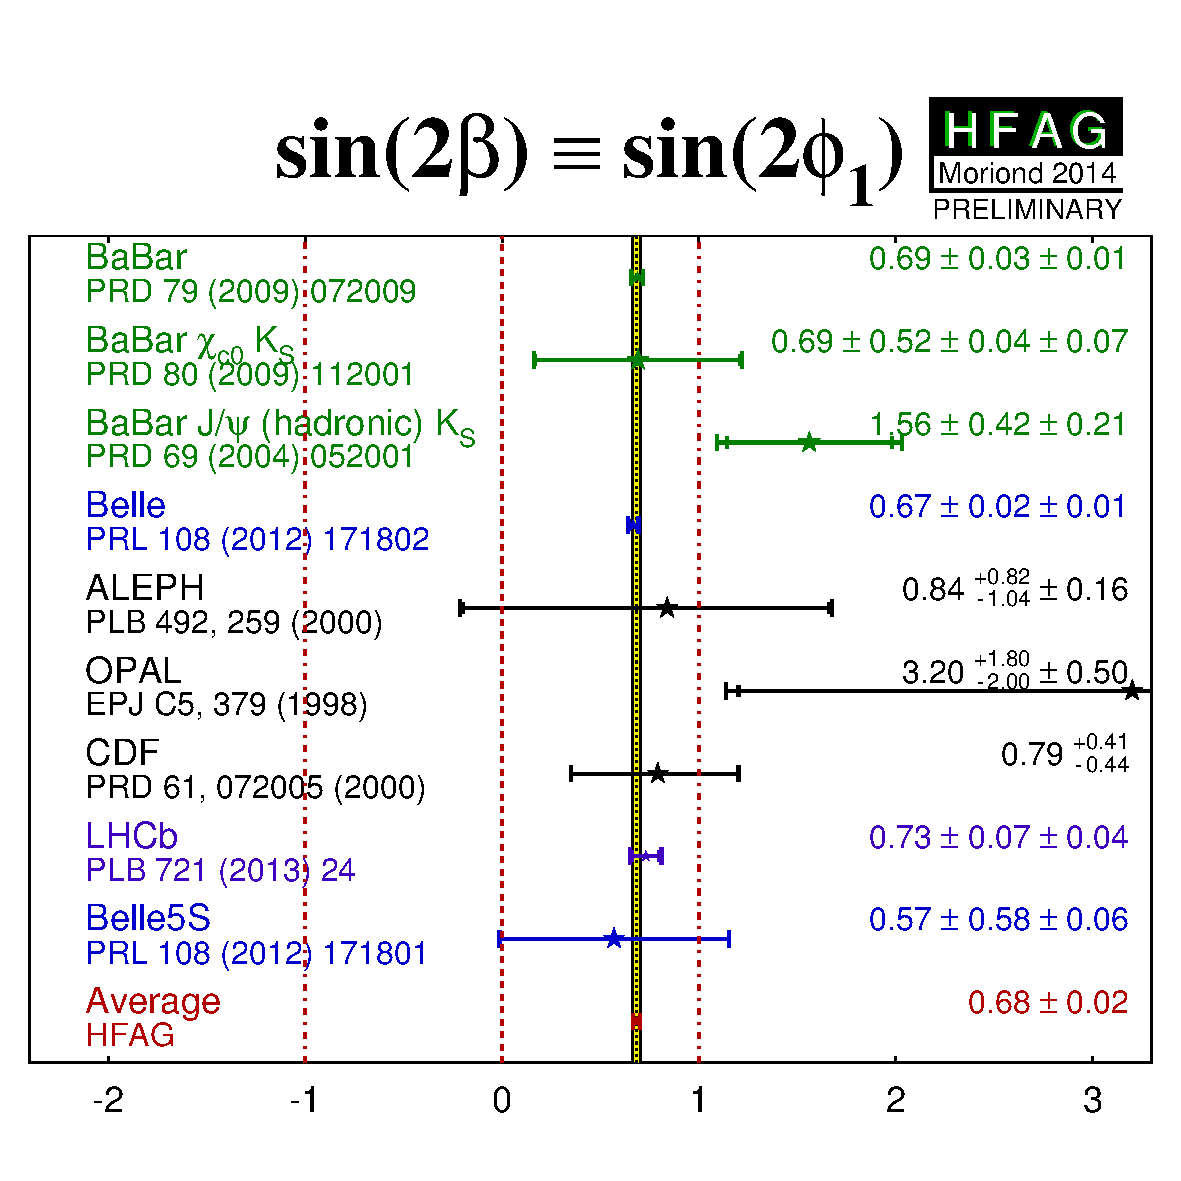
\includegraphics{figures/cp_uta/btoccsS_CP}
    }
    \hfill
    \resizebox{0.48\textwidth}{!}{
      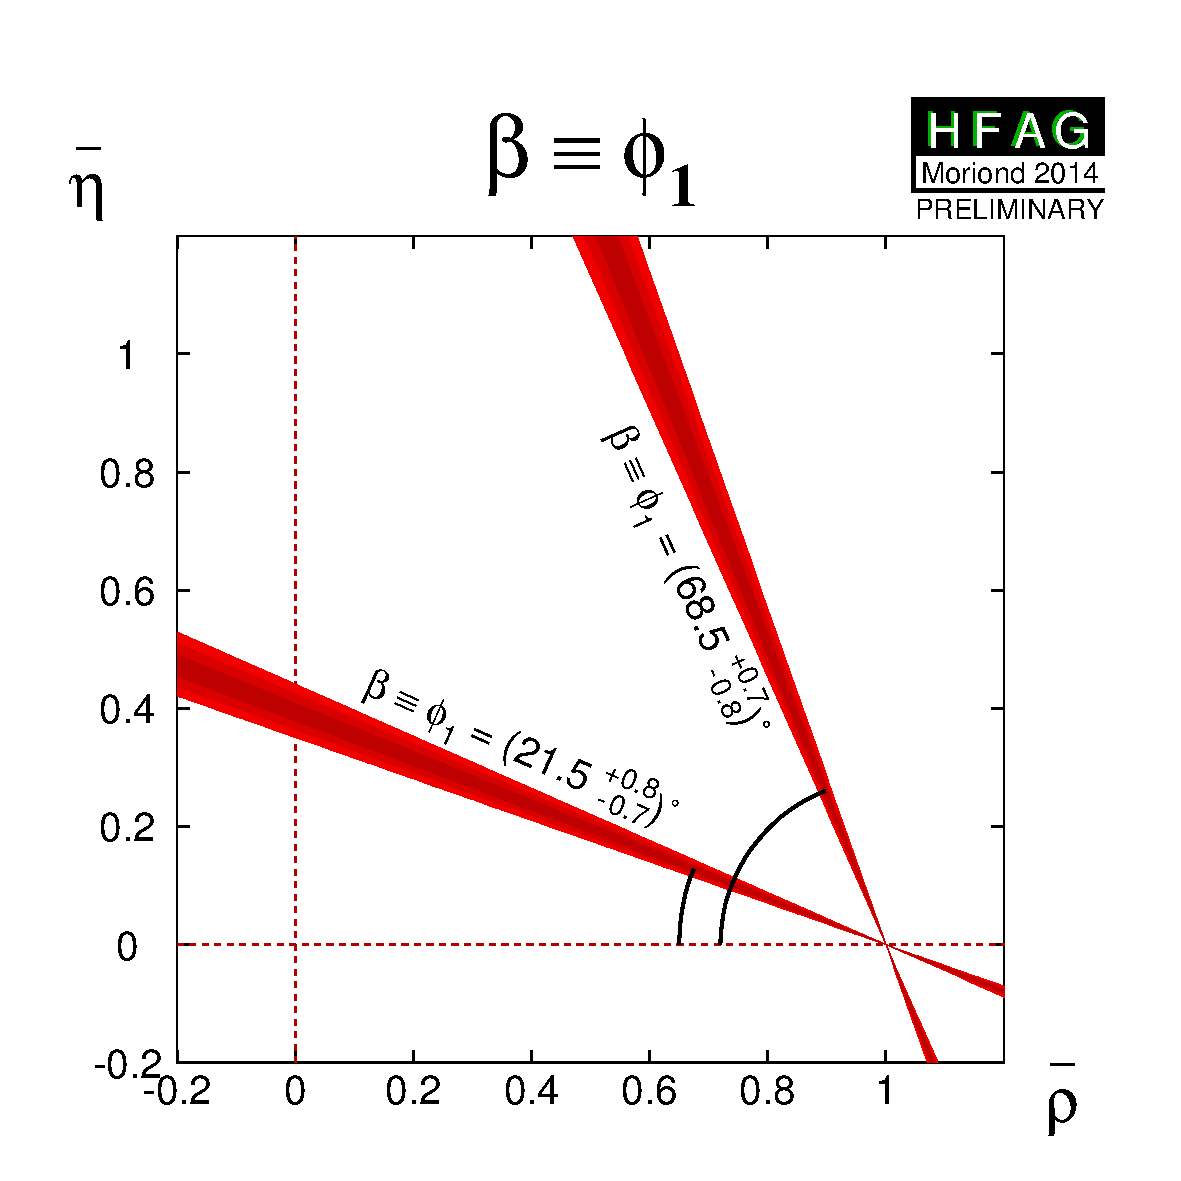
\includegraphics{figures/cp_uta/phi1_rhoBar_etaBar}
    }
  \end{center}
  \vspace{-0.5cm}
  \caption{
    (Left) Average of measurements of $S_{b \to c\bar c s}$.
    (Right) Constraints on the $(\rhobar,\etabar)$ plane,
    obtained from the average of $-\etacp S_{b \to c\bar c s}$ 
    and Eq.~\ref{eq:cp_uta:sin2beta}.
  }
  \label{fig:cp_uta:ccs}
\end{figure}

%%%%%%%%
%%%
%%% J/psiK*
%%%
%%%%%%%%
\mysubsubsection{Time-dependent transversity analysis of $\Bz \to J/\psi K^{*0}$
}
\label{sec:cp_uta:ccs:vv}

$\B$ meson decays to the vector-vector final state $J/\psi K^{*0}$
are also mediated by the $b \to c \bar c s$ transition.
When a final state which is not flavour-specific ($K^{*0} \to \KS \pi^0$) is used,
a time-dependent transversity analysis can be performed 
allowing sensitivity to both 
$\sin(2\beta)$ and $\cos(2\beta)$~\cite{Dunietz:1990cj}.
Such analyses have been performed by both $\B$ factory experiments.
In principle, the strong phases between the transversity amplitudes
are not uniquely determined by such an analysis, 
leading to a discrete ambiguity in the sign of $\cos(2\beta)$.
The \babar\ collaboration resolves 
this ambiguity using the known variation~\cite{Aston:1987ir}
of the P-wave phase (fast) relative to the S-wave phase (slow) 
with the invariant mass of the $K\pi$ system 
in the vicinity of the $K^*(892)$ resonance. 
The result is in agreement with the prediction from 
$s$ quark helicity conservation,
and corresponds to Solution II defined by Suzuki~\cite{Suzuki:2001za}.
We use this phase convention for the averages given in 
Table~\ref{tab:cp_uta:ccs:psi_kstar} and Fig.~\ref{fig:cp_uta:JpsiKstar}.

\begin{table}[htb]
	\begin{center}
		\caption{
			Averages from $\Bz \to J/\psi K^{*0}$ transversity analyses.
		}
		\vspace{0.2cm}
		\setlength{\tabcolsep}{0.0pc}
		\begin{tabular*}{\textwidth}{@{\extracolsep{\fill}}lrcccc} \hline
		\mc{2}{l}{Experiment} & $N(B\bar{B})$ & $\sin 2\beta$ & $\cos 2\beta$ & Correlation \\
		\hline
	\babar & \cite{Aubert:2004cp} & 88M & $-0.10 \pm 0.57 \pm 0.14$ & $3.32 ^{+0.76}_{-0.96} \pm 0.27$ & $-0.37$ \\
	\belle & \cite{Itoh:2005ks} & 275M & $0.24 \pm 0.31 \pm 0.05$ & $0.56 \pm 0.79 \pm 0.11$ & $0.22$ \\
%	\hline
	\mc{3}{l}{\bf Average} & $0.16 \pm 0.28$ & $1.64 \pm 0.62$ &  \hspace{-8mm} {\small uncorrelated averages}  \\
        \mc{3}{l}{\small Confidence level} & {\small $0.61~(0.5\sigma)$} & {\small $0.03~(2.2\sigma)$} & \\
		\hline
		\end{tabular*}
		\label{tab:cp_uta:ccs:psi_kstar}
	\end{center}
\end{table}




At present the results are dominated by 
large and non-Gaussian statistical errors,
and exhibit significant correlations.
We perform uncorrelated averages, 
the interpretation of which has to be done with the greatest care. 
Nonetheless, it is clear that $\cos(2\beta)>0$ is preferred 
by the experimental data in $J/\psi \Kstarz$.
[\babar~\cite{Aubert:2004cp} 
find a confidence level for $\cos(2\beta)>0$ of $89\%$.]

\begin{figure}[htb]
  \begin{center}
    \resizebox{0.46\textwidth}{!}{
      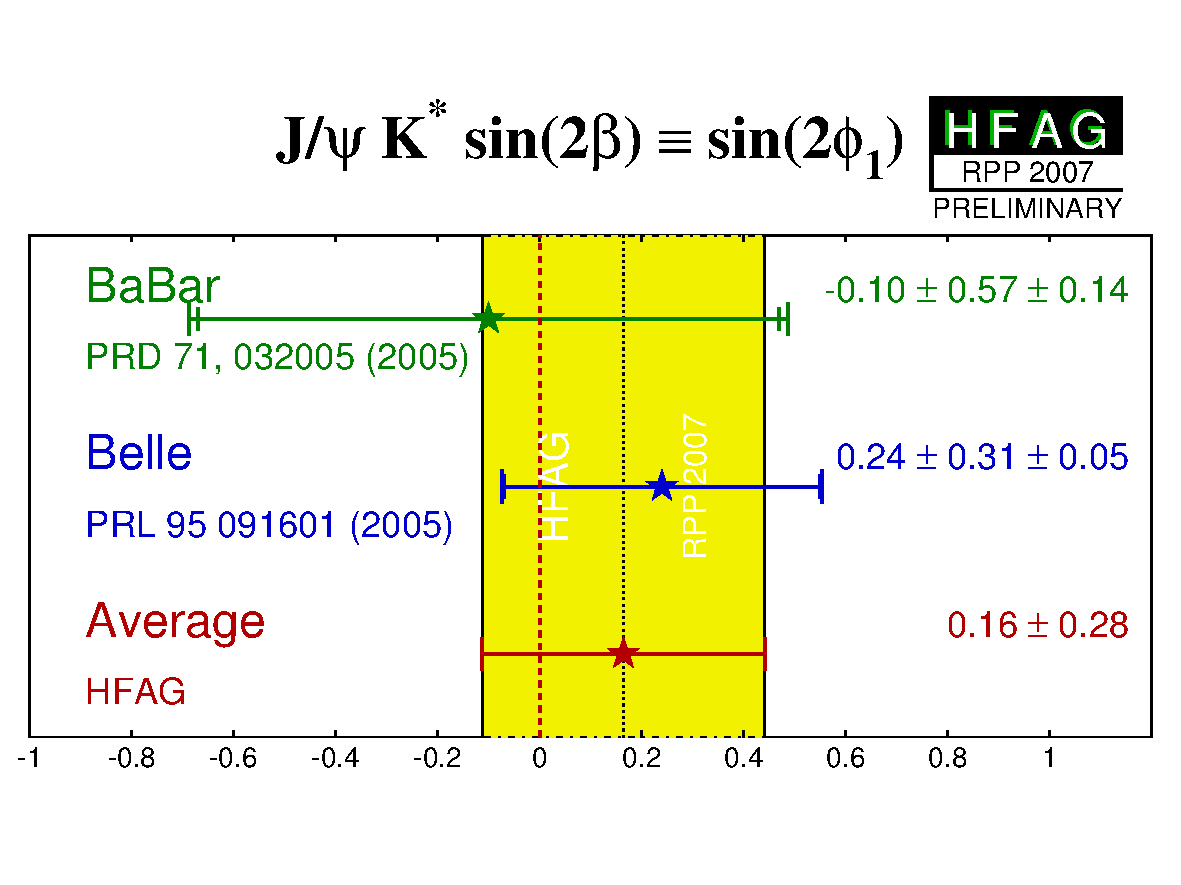
\includegraphics{figures/cp_uta/JpsiKstarsin2beta}
    }
    \hfill
    \resizebox{0.46\textwidth}{!}{
      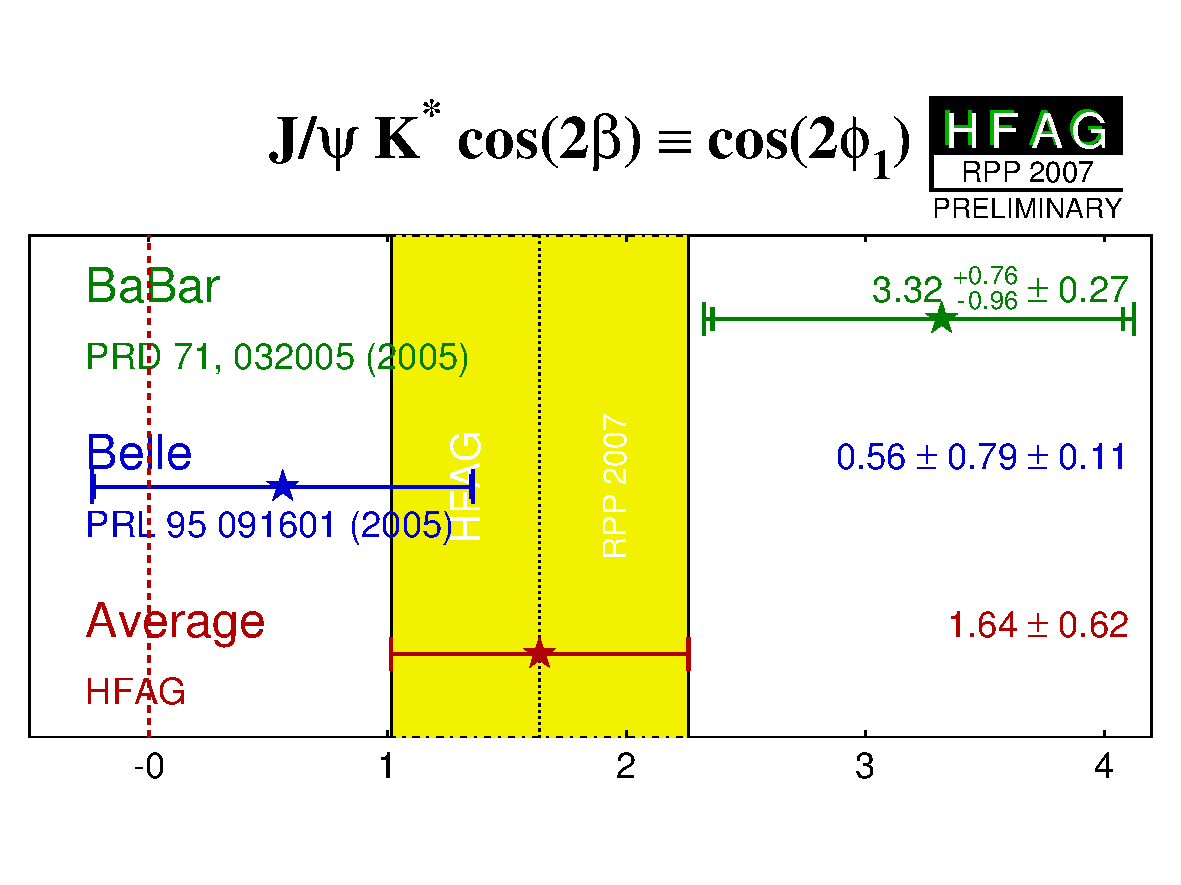
\includegraphics{figures/cp_uta/JpsiKstarcos2beta}
    }
  \end{center}
  \vspace{-0.5cm}
  \caption{
    Averages of 
    (left) $\sin(2\beta) \equiv \sin(2\phi_1)$ and
    (right) $\cos(2\beta) \equiv \cos(2\phi_1)$
    from time-dependent analyses of $\Bz \to \jpsi K^{*0}$ decays.
  }
  \label{fig:cp_uta:JpsiKstar}
\end{figure}

%%%%%%%%
%%%
%%% D*D*Ks
%%%
%%%%%%%%
\mysubsubsection{Time-dependent $\CP$ asymmetries in $\Bz \to \Dstarp \Dstarm \KS$ decays
}
\label{sec:cp_uta:ccs:DstarDstarKs}

Both \babar~\cite{Aubert:2006fh} and \belle~\cite{Dalseno:2007hx} have performed
time-dependent analyses of the $\Bz \to \Dstarp \Dstarm \KS$ decay,
to obtain information on the sign of $\cos(2\beta)$.
More information can be found in 
Sec.~\ref{sec:cp_uta:notations:dalitz:dstardstarks}.
The results are shown in Table~\ref{tab:cp_uta:ccs:dstardstarks}, 
and Fig.~\ref{fig:cp_uta:ccs:dstardstarks}.

\begin{table}[htb]
	\begin{center}
		\caption{
                        Results from time-dependent analysis of $\Bz \to \Dstarp \Dstarm \KS$.
		}
		\vspace{0.2cm}
		\setlength{\tabcolsep}{0.0pc}
		\begin{tabular*}{\textwidth}{@{\extracolsep{\fill}}lrcccc} \hline
                \mc{2}{l}{Experiment} & $N(B\bar{B})$ & $\frac{J_c}{J_0}$ & $\frac{2J_{s1}}{J_0} \sin(2\beta)$ &  $\frac{2J_{s2}}{J_0} \cos(2\beta)$ \\
		\hline
	\babar & \cite{Aubert:2006fh} & 230M & $0.76 \pm 0.18 \pm 0.07$ & $0.10 \pm 0.24 \pm 0.06$ & $0.38 \pm 0.24 \pm 0.05$ \\
	\belle & \cite{Dalseno:2007hx} & 449M & $0.60 \,^{+0.25}_{-0.28} \pm 0.08$ & $-0.17 \pm 0.42 \pm 0.09$ & $-0.23 \,^{+0.43}_{-0.41} \pm 0.13$ \\
%	\hline
	\mc{3}{l}{\bf Average} & $0.71 \pm 0.16$ & $0.03 \pm 0.21$ & $0.24 \pm 0.22$ \\
	\mc{3}{l}{\small Confidence level} & {\small $0.63~(0.5\sigma)$} & {\small $0.59~(0.5\sigma)$} & {\small $0.23~(1.2\sigma)$} \\
		\hline
		\end{tabular*}
		\label{tab:cp_uta:ccs:dstardstarks}
	\end{center}
\end{table}




\begin{figure}[htb]
  \begin{center}
    \begin{tabular}{c@{\hspace{-1mm}}c@{\hspace{-1mm}}c}
      \resizebox{0.32\textwidth}{!}{
        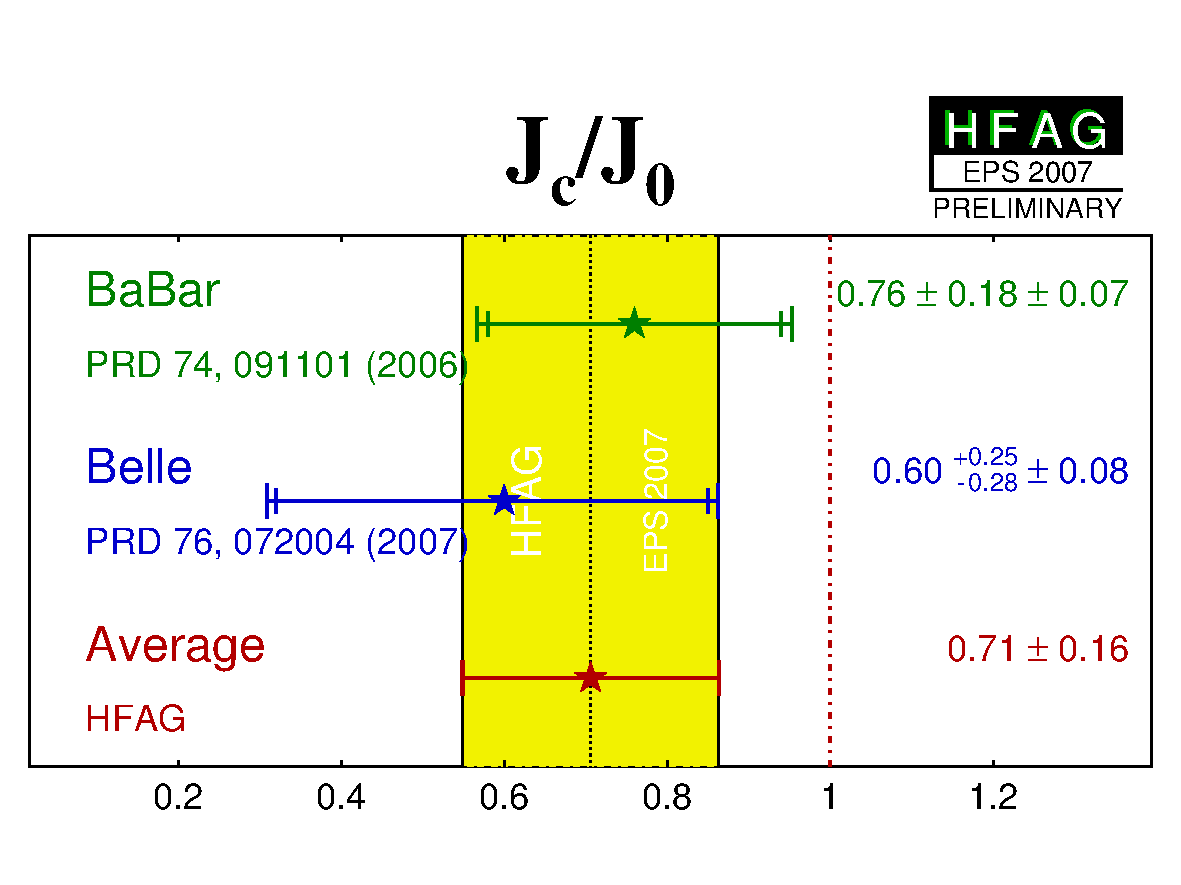
\includegraphics{figures/cp_uta/DstarDstarKSJcJ0}
      }
      &
      \resizebox{0.32\textwidth}{!}{
        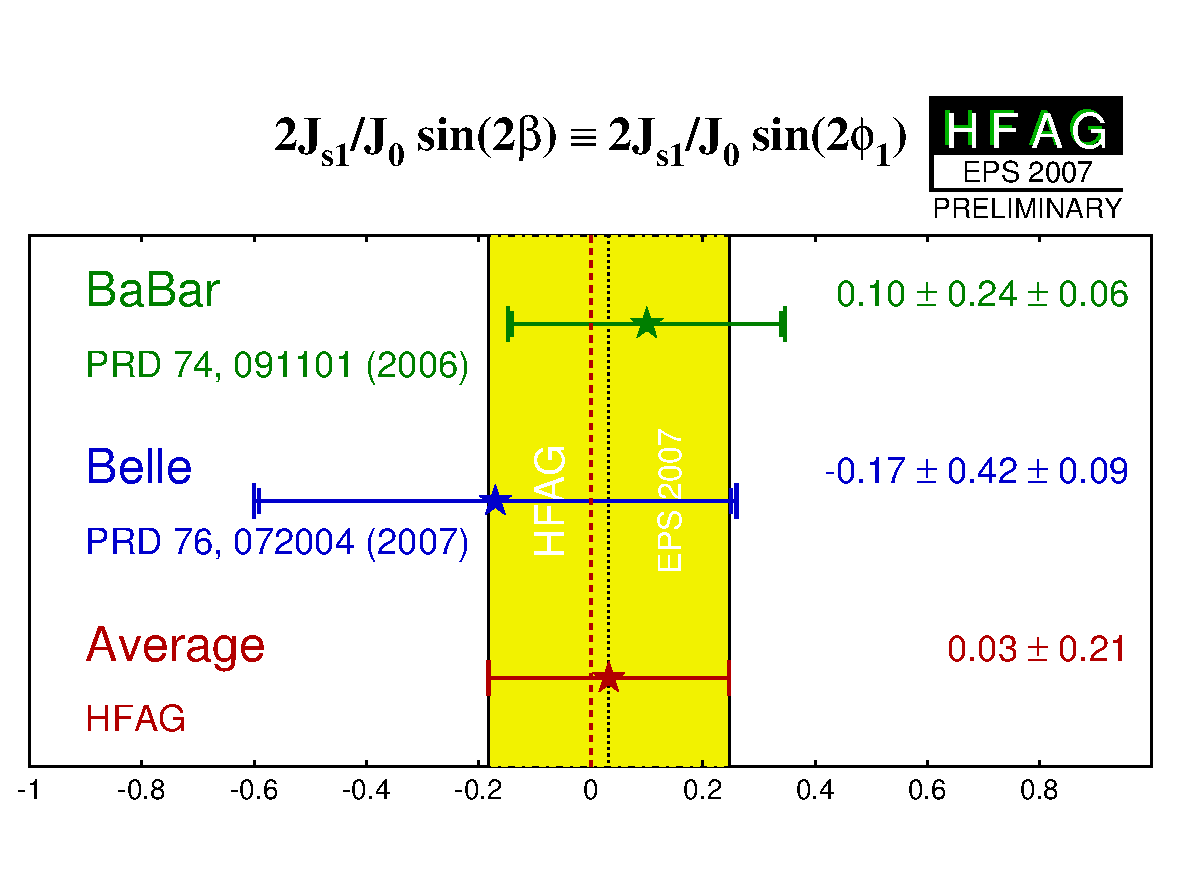
\includegraphics{figures/cp_uta/DstarDstarKS2Js1J0-s}
      }
      &
      \resizebox{0.32\textwidth}{!}{
        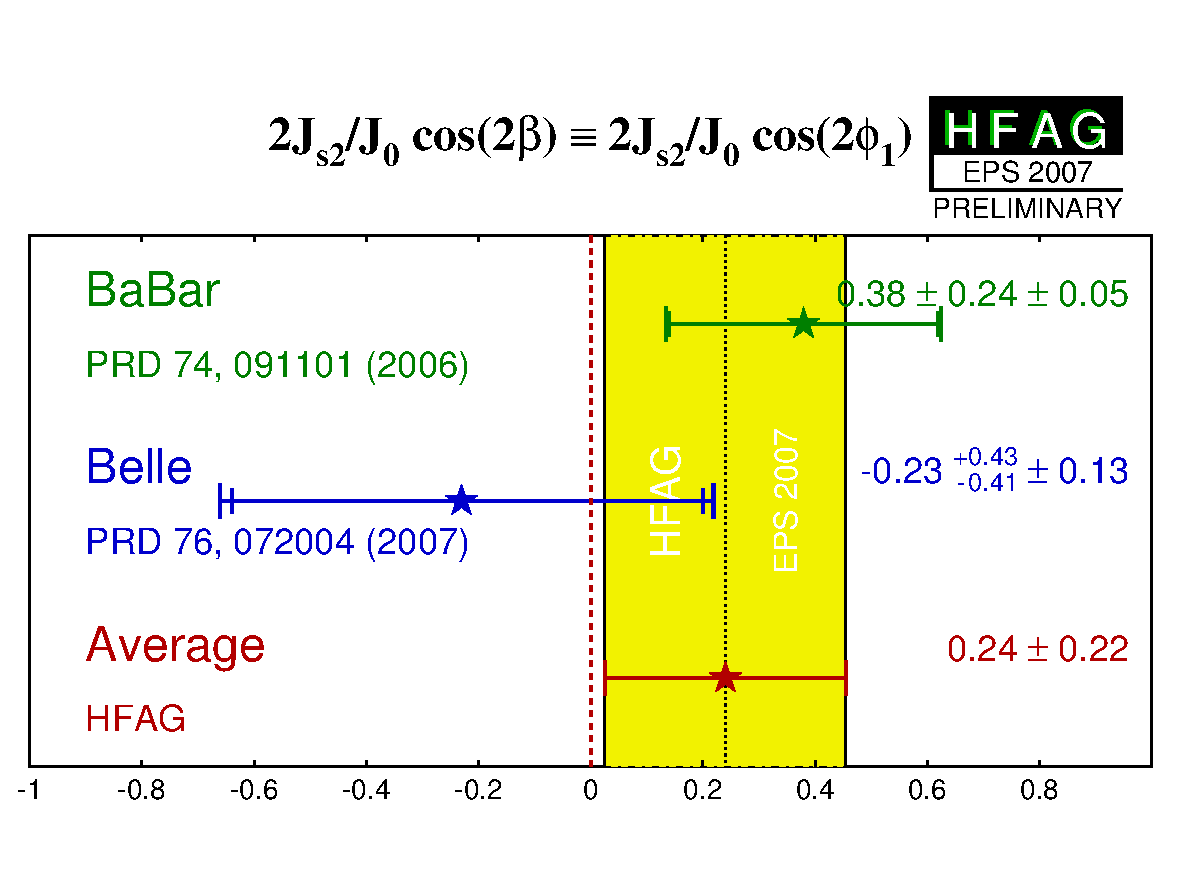
\includegraphics{figures/cp_uta/DstarDstarKS2Js2J0-c}
      }
    \end{tabular}
  \end{center}
  \vspace{-0.8cm}
  \caption{
    Averages of 
    (left) $(J_c/J_0)$, (middle) $(2J_{s1}/J_0) \sin(2\beta)$ and 
    (right) $(2J_{s2}/J_0) \cos(2\beta)$
    from time-dependent analyses of $\Bz \to \Dstarp \Dstarm \KS$ decays.
  }
  \label{fig:cp_uta:ccs:dstardstarks}
\end{figure}

From the above result and the assumption that $J_{s2}>0$, 
\babar\ infer that $\cos(2\beta)>0$ at the $94\%$ confidence level~\cite{Aubert:2006fh}.

%%%%%%%%
%%%
%%% Bs -> J/psi phi
%%%
%%%%%%%%
\mysubsubsection{Time-dependent analysis of $\Bs$ decays though the $b to c\bar{c}s$ transition
}
\label{sec:cp_uta:ccs:jpsiphi}

As described in Sec.~\ref{sec:cp_uta:notations:Bs},
time-dependent analysis of decays such as $\Bs \to J/\psi \phi$ probes the 
$\CP$ violating phase of $\Bs$--$\Bsbar$ oscillations, $\phi_s$.
Within the Standard Model, this parameter is predicted to be small.\footnote{
   We make the approximation $\phi_s = -2 \beta_s$, 
   where $\phi_s \equiv \arg\left[ -M_{12}/\Gamma_{12} \right]$ 
   and $2\beta_s \equiv 2 \arg\left[ -(V_{ts}V_{tb}^*)/(V_{cs}V_{cb}^*) \right]$
   (see Section~\ref{sec:cp_uta:introduction}). 
   This is a reasonable approximation since, 
   although the equality does not hold in the Standard Model~\cite{Lenz:2011ti,*Lenz:2006hd}, 
   both are much smaller than the current experimental resolution, 
   whereas new physics contributions add a phase $\phi_{\rm NP}$ to $\phi_s$
   and subtract the same phase from $2\beta_s$, 
   so that the approximation remains valid.
}
The combination of results on $\Bs \to \jpsi \phi$ decays, including also results from $\Bs \to \jpsi \pi^+\pi^-$ and $\Bs \to D_s^+D_s^-$ decays, is performed by the HFAG Lifetimes and Oscillations group, see Sec.~\ref{sec:life_mix}.

%%%%%%%%
%%%
%%% Dh0
%%%
%%%%%%%%
\clearpage
\mysubsection{Time-dependent $\CP$ asymmetries in colour-suppressed $b \to c\bar{u}d$ transitions
}
\label{sec:cp_uta:cud_beta}

Decays of $\B$ mesons to final states such as $D\pi^0$ are 
governed by $b \to c\bar{u}d$ transitions. 
If the final state is a $\CP$ eigenstate, \eg\ $D_{\CP}\pi^0$, 
the usual time-dependence formulae are recovered, 
with the sine coefficient sensitive to $\sin(2\beta)$. 
Since there is no penguin contribution to these decays, 
there is even less associated theoretical uncertainty 
than for $b \to c\bar{c}s$ decays like $\B \to \jpsi \KS$.
Such measurements therefore allow to test the Standard Model prediction
that the $\CP$ violation parameters in $b \to c\bar{u}d$ transitions
are the same as those in $b \to c\bar{c}s$~\cite{Grossman:1996ke}.

Note that there is an additional contribution from CKM suppressed
$b \to u \bar{c} d$ decays.
The effect of this contribution is small, and can be taken into 
account in the analysis~\cite{Fleischer:2003ai,Fleischer:2003aj}.

Results of such an analysis are available from \babar~\cite{Aubert:2007mn}.
The decays $\Bz \to D\pi^0$, $\Bz \to D\eta$, $\Bz \to D\omega$,
$\Bz \to D^*\pi^0$ and $\Bz \to D^*\eta$ are used.
The daughter decay $D^* \to D\pi^0$ is used.
The $\CP$-even $D$ decay to $K^+K^-$ is used for all decay modes,
with the $\CP$-odd $D$ decay to $\KS\omega$ also used in $\Bz \to D^{(*)}\pi^0$
and the additional $\CP$-odd $D$ decay to $\KS\pi^0$ 
also used in $\Bz \to D\omega$.
Results are presented separately for $\CP$-even and $\CP$-odd 
$D^{(*)}$ decays (denoted $D^{(*)}_+ h^0$ and $D^{(*)}_- h^0$ respectively),
and for both combined, with the different $\CP$ factors accounted for
(denoted $D^{(*)}_{\CP} h^0$).
The results are summarised in Table~\ref{tab:cp_uta:cud_cp_beta}.

\begin{table}[htb]
	\begin{center}
		\caption{
			Results from analyses of $\Bz \to D^{(*)}h^0$, $D \to CP$ eigenstates decays.
		}
		\vspace{0.2cm}
		\setlength{\tabcolsep}{0.0pc}
		\begin{tabular*}{\textwidth}{@{\extracolsep{\fill}}lrcccc} \hline
	\mc{2}{l}{Experiment} & $N(B\bar{B})$ & $S_{CP}$ & $C_{CP}$ & Correlation \\
	\hline
        \mc{6}{c}{$D^{(*)}_+ h^0$}  \\
	\babar & \cite{Aubert:2007mn} & 383M & $-0.65 \pm 0.26 \pm 0.06$ & $-0.33 \pm 0.19 \pm 0.04$ & $0.04$ \\
	\hline
%		\end{tabular*}
% 		\label{tab:cp_uta:yyy}
% 	\end{center}
% \end{table}


% \begin{table}[htb]
% 	\begin{center}
% 		\caption{
% 			Averages for $D_- h0$.
% 		}
% 		\vspace{0.2cm}
% 		\setlength{\tabcolsep}{0.0pc}
% 		\begin{tabular*}{\textwidth}{@{\extracolsep{\fill}}lrcccc} \hline
% 	\mc{2}{l}{Experiment} & $N(B\bar{B})$ & $S_{CP}$ & $C_{CP}$ & Correlation \\
%         \hline
        \mc{6}{c}{$D^{(*)}_- h^0$} \\
	\babar & \cite{Aubert:2007mn} & 383M & $-0.46 \pm 0.46 \pm 0.13$ & $-0.03 \pm 0.28 \pm 0.07$ & $-0.14$ \\
	\hline
%		\end{tabular*}
% 		\label{tab:cp_uta:yyy}
% 	\end{center}
% \end{table}


% \begin{table}[htb]
% 	\begin{center}
% 		\caption{
% 			Averages for $D h0$.
% 		}
% 		\vspace{0.2cm}
% 		\setlength{\tabcolsep}{0.0pc}
% 		\begin{tabular*}{\textwidth}{@{\extracolsep{\fill}}lrcccc} \hline
% 	\mc{2}{l}{Experiment} & $N(B\bar{B})$ & $S_{CP}$ & $C_{CP}$ & Correlation \\
%         \hline
        \mc{6}{c}{$D^{(*)}_{CP} h^0$} \\
	\babar & \cite{Aubert:2007mn} & 383M & $-0.56 \pm 0.23 \pm 0.05$ & $-0.23 \pm 0.16 \pm 0.04$ & $-0.02$ \\
	\hline
		\end{tabular*}
		\label{tab:cp_uta:cud_cp_beta}
	\end{center}
\end{table}



When multibody $D$ decays, such as $D \to \KS\pi^+\pi^-$ are used, 
a time-dependent analysis of the Dalitz plot of the neutral $D$ decay 
allows a direct determination of the weak phase: $2\beta$. 
(Equivalently, both $\sin(2\beta)$ and $\cos(2\beta)$ can be measured.)
This information allows to resolve the ambiguity in the 
measurement of $2\beta$ from $\sin(2\beta)$~\cite{Bondar:2005gk}.

Results of such analyses are available from both 
\belle~\cite{Krokovny:2006sv} and \babar~\cite{Aubert:2007rp}.
The decays $\B \to D\pi^0$, $\B \to D\eta$, $\B \to D\omega$, 
$\B \to D^*\pi^0$ and $\B \to D^*\eta$ are used. 
[This collection of states is denoted by $D^{(*)}h^0$.]
The daughter decays are $D^* \to D\pi^0$ and $D \to \KS\pi^+\pi^-$.
The results are shown in Table~\ref{tab:cp_uta:cud_beta},
and Fig.~\ref{fig:cp_uta:cud_beta}.
Note that \babar\ quote uncertainties due to the $D$ decay model 
separately from other systematic errors, while \belle\ do not.

\begin{table}[htb]
	\begin{center}
		\caption{
			Averages from $\Bz \to D^{(*)}h^0$, $D \to K_S\pi^+\pi^-$ analyses.
		}
		\vspace{0.2cm}
		\setlength{\tabcolsep}{0.0pc}
    \resizebox{\textwidth}{!}{
      		\begin{tabular*}{\textwidth}{@{\extracolsep{\fill}}lrcccc} \hline
	\mc{2}{l}{Experiment} & $N(B\bar{B})$ & $\sin 2\beta$ & $\cos 2\beta$ & $|\lambda|$ \\
		\hline
	\babar & \cite{Aubert:2007rp} & 383M & $0.29 \pm 0.34 \pm 0.03 \pm 0.05$ & $0.42 \pm 0.49 \pm 0.09 \pm 0.13$ & $1.01 \pm 0.08 \pm 0.02$ \\
	\belle & \cite{Krokovny:2006sv} & 386M & $0.78 \pm 0.44 \pm 0.22$ & $1.87 \,^{+0.40}_{-0.53} \,^{+0.22}_{-0.32}$ & \textendash{} \\
%	\hline
	\mc{3}{l}{\bf Average} & $0.45 \pm 0.28$ & $1.01 \pm 0.40$ & $1.01 \pm 0.08$ \\
	\mc{3}{l}{\small Confidence level} & {\small $0.59~(0.5\sigma)$} & {\small $0.12~(1.6\sigma)$} & \textendash{} \\
		\hline
		\end{tabular*}
    }
		\label{tab:cp_uta:cud_beta}
	\end{center}
\end{table}




Again, it is clear that the data prefer $\cos(2\beta)>0$.
Indeed, \belle~\cite{Krokovny:2006sv} 
determine the sign of $\cos(2\phi_1)$ to be positive at $98.3\%$ confidence level,
while \babar~\cite{Aubert:2007rp} 
favour the solution of $\beta$ with $\cos(2\beta)>0$ at $87\%$ confidence level.
Note, however, that the Belle measurement has strongly non-Gaussian behaviour. 
Therefore, we perform uncorrelated averages, 
from which any interpretation has to be done with the greatest care. 

\begin{figure}[htb]
  \begin{center}
    \begin{tabular}{cc}
      \resizebox{0.46\textwidth}{!}{
        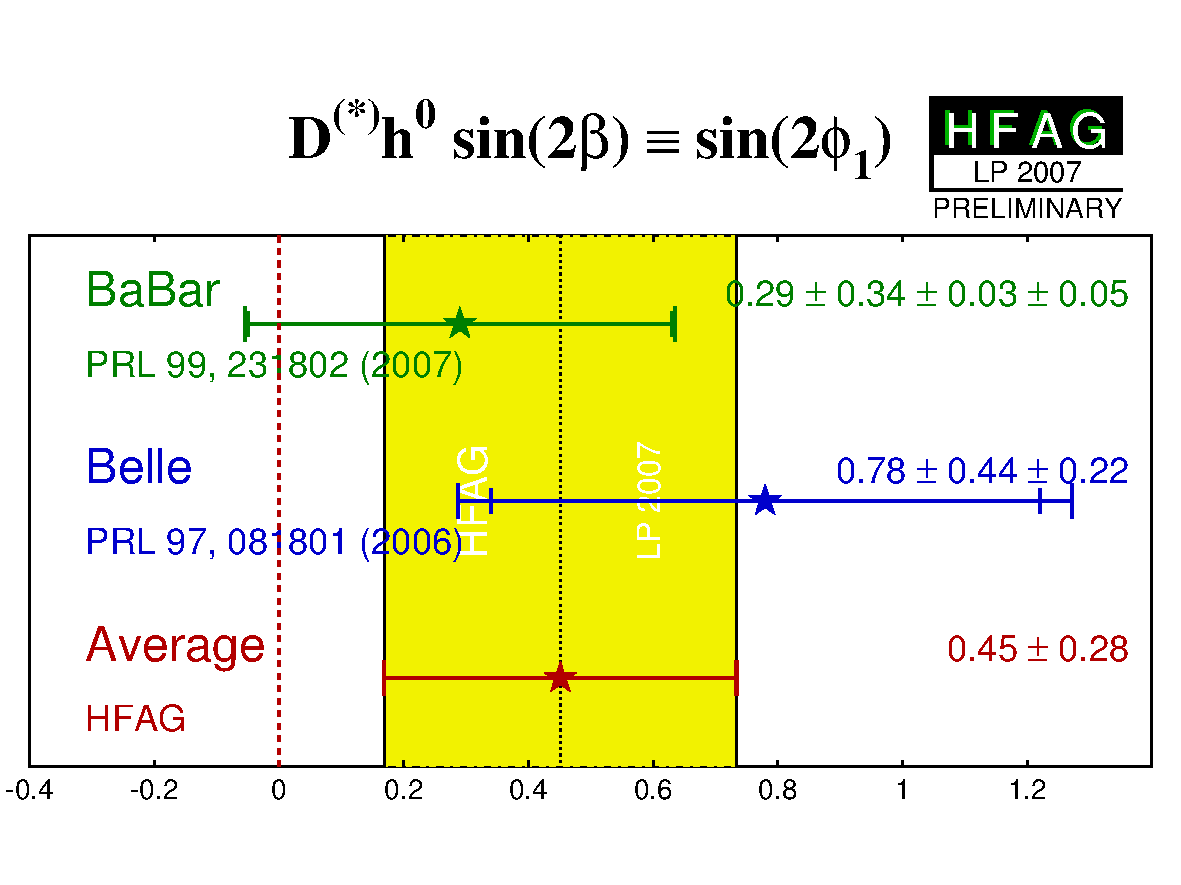
\includegraphics{figures/cp_uta/Dh0sin2beta}
      }
      &
      \resizebox{0.46\textwidth}{!}{
        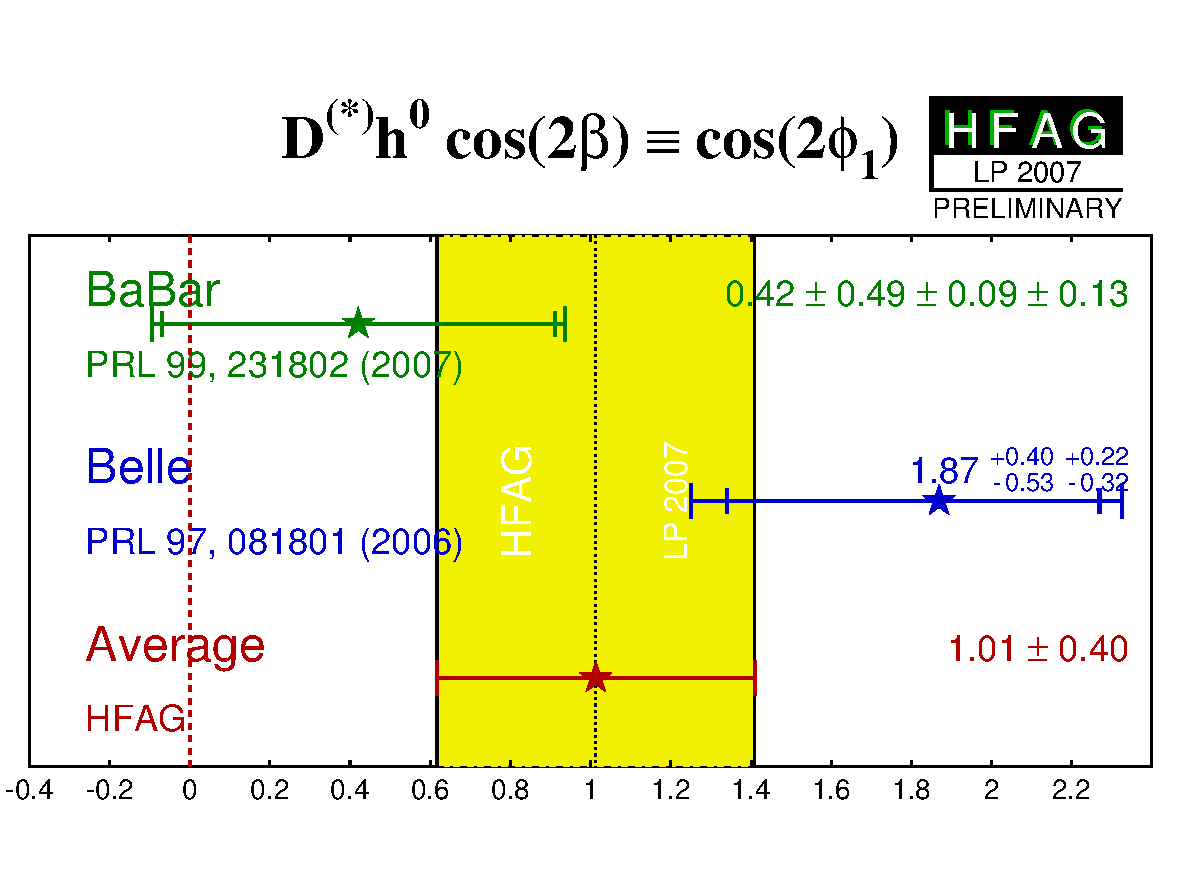
\includegraphics{figures/cp_uta/Dh0cos2beta}
      }
    \end{tabular}
  \end{center}
  \vspace{-0.8cm}
  \caption{
    Averages of 
    (left) $\sin(2\beta)$ and (right) $\cos(2\beta)$
    measured in colour-suppressed $b \to c\bar{u}d$ transitions.
  }
  \label{fig:cp_uta:cud_beta}
\end{figure}

%%%%%%%%
%%%
%%% qqs
%%%
%%%%%%%%
\clearpage
\mysubsection{Time-dependent $\CP$ asymmetries in charmless $b \to q\bar{q}s$ transitions
}
\label{sec:cp_uta:qqs}

The flavour changing neutral current $b \to s$ penguin
can be mediated by any up-type quark in the loop, 
and hence the amplitude can be written as
\begin{equation}
  \label{eq:cp_uta:b_to_s}
  \begin{array}{ccccc}
    A_{b \to s} & = & 
    \mc{3}{l}{F_u V_{ub}V^*_{us} + F_c V_{cb}V^*_{cs} + F_t V_{tb}V^*_{ts}} \\
    & = & (F_u - F_c) V_{ub}V^*_{us} & + & (F_t - F_c) V_{tb}V^*_{ts} \\
    & = & {\cal O}(\lambda^4) & + & {\cal O}(\lambda^2) \\
  \end{array}
\end{equation}
using the unitarity of the CKM matrix.
Therefore, in the Standard Model, 
this amplitude is dominated by $V_{tb}V^*_{ts}$, 
and to within a few degrees 
($\delta\beta \lesssim 2^\circ$ for $\beta \approx 20^\circ$) 
the time-dependent parameters can be written\footnote
{
  The presence of a small (${\cal O}(\lambda^2)$) weak phase in 
  the dominant amplitude of the $s$ penguin decays introduces 
  a phase shift given by
  $S_{b \to q\bar q s} = -\eta\sin(2\beta)\cdot(1 + \Delta)$. 
  Using the CKMfitter results for the Wolfenstein 
  parameters~\cite{Charles:2004jd}, one finds: 
  $\Delta \simeq 0.033$, which corresponds to a shift of 
  $2\beta$ of $+2.1$ degrees. 
  Nonperturbative contributions can alter this result.
}
$S_{b \to q\bar q s} \approx - \etacp \sin(2\beta)$,
$C_{b \to q\bar q s} \approx 0$,
assuming $b \to s$ penguin contributions only ($q = u,d,s$).

Due to the large virtual mass scales occurring in the penguin loops,
additional diagrams from physics beyond the Standard Model,
with heavy particles in the loops, may contribute.
In general, these contributions will affect the values of 
$S_{b \to q\bar q s}$ and $C_{b \to q\bar q s}$.
A discrepancy between the values of 
$S_{b \to c\bar c s}$ and $S_{b \to q\bar q s}$
can therefore provide a clean indication of new physics~\cite{Grossman:1996ke,Fleischer:1996bv,London:1997zk,Ciuchini:1997zp}.

However, there is an additional consideration to take into account.
The above argument assumes only the $b \to s$ penguin contributes
to the $b \to q\bar q s$ transition.
For $q = s$ this is a good assumption, which neglects only rescattering effects.
However, for $q = u$ there is a colour-suppressed $b \to u$ tree diagram
(of order ${\cal O}(\lambda^4)$), 
which has a different weak (and possibly strong) phase.
In the case $q = d$, any light neutral meson that is formed from $d \bar{d}$ 
also has a $u \bar{u}$ component, and so again there is ``tree pollution''. 
The \Bz decays to $\piz\KS$, $\rho^0\KS$ and $\omega\KS$ belong to this category.
The mesons $\phi$, $f_0$ and $\etapr$ are expected to have predominant
$s\bar{s}$ parts, which reduces the relative size of the possible tree
pollution. 
If the inclusive decay $\Bz\to\Kp\Km\Kz$ (excluding $\phi\Kz$) is dominated by
a nonresonant three-body transition, 
an OZI-rule suppressed tree-level diagram can occur 
through insertion of an $s\sbar$ pair. 
The corresponding penguin-type transition 
proceeds via insertion of a $u\ubar$ pair, which is expected
to be favoured over the $s\sbar$ insertion by fragmentation models.
Neglecting rescattering, the final state $\Kz\Kzb\Kz$ 
(reconstructed as $\KS\KS\KS$) has no tree pollution~\cite{Gershon:2004tk}.
%% this is repeated below
% Note that the calculation of an average between different modes
% implicitly neglects contributions with different weak phases 
% to the $b \to s$ penguin amplitude.
Various estimates, using different theoretical approaches,
of the values of $\Delta S = S_{b \to q\bar q s} - S_{b \to c\bar c s}$
exist in the literature~\cite{Grossman:2003qp,Gronau:2003ep,Gronau:2003kx,Gronau:2004hp,Cheng:2005bg,Gronau:2005gz,Buchalla:2005us,Beneke:2005pu,Engelhard:2005hu,Cheng:2005ug,Engelhard:2005ky,Gronau:2006qh,Silvestrini:2007yf,Dutta:2008xw}.
In general, there is agreement that the modes
$\phi\Kz$, $\etapr\Kz$ and $\Kz\Kzb\Kz$ are the cleanest,
with values of $\left| \Delta S \right|$ at or below the few percent level 
($\Delta S$ is usually positive).

\mysubsubsection{Time-dependent $\CP$ asymmetries: $b \to q\bar{q}s$ decays to $\CP$ eigenstates
}
\label{sec:cp_uta:qqs:cp_eigen}

The averages for $-\etacp S_{b \to q\bar q s}$ and $C_{b \to q\bar q s}$
can be found in Table~\ref{tab:cp_uta:qqs},
and are shown in Figs.~\ref{fig:cp_uta:qqs},~\ref{fig:cp_uta:qqs_SvsC} 
and~\ref{fig:cp_uta:qqs_SvsC-all}.
Results from both \babar\  and \belle\ are averaged for the modes
$\etapr\Kz$ ($\Kz$ indicates that both $\KS$ and $\KL$ are used)
$\KS\KS\KS$, $\pi^0 \KS$ and $\omega\KS$.\footnote{
  \belle~\cite{Fujikawa:2008pk} include the $\pi^0\KL$ final state together with $\pi^0 \KS$ in order to improve the constraint on the parameter of \CP\ violation in decay; these events cannot be used for time-dependent analysis.
}
Results on $\phi\KS$ and $\Kp\Km\KS$ (implicitly excluding $\phi\KS$ and $f_0\KS$) are taken from time-dependent Dalitz plot analyses of $\Kp\Km\KS$;
results on $\rho^0\KS$, $f_2\KS$, $f_{\rm X}\KS$ and $\pip\pim\KS$ nonresonant are taken from time-dependent Dalitz plot analyses of $\pip\pim\KS$ (see
subsection~\ref{sec:cp_uta:qqs:dp}).
The results on $f_0\KS$ are from combinations of both Dalitz plot analyses.
\babar\ also has presented results with the final states
$\pi^0\pi^0\KS$,\footnote{
  We do not include a preliminary result from \belle~\cite{:2007xd}, which
  remains unpublished after more than two years.
}
and $\phi \KS \pi^0$. 

Of these final states,
$\phi\KS$, $\etapr\KS$, $\pi^0 \KS$, $\rho^0\KS$, $\omega\KS$ and $f_0\KL$
have $\CP$ eigenvalue $\etacp = -1$, 
while $\phi\KL$, $\etapr\KL$, $\KS\KS\KS$, $f_0 \KS$, $f_2 \KS$, 
$f_{\rm X} \KS$,\footnote{ 
  The $f_{\rm X}$ is assumed to be spin even.
} $\pi^0\pi^0\KS$ and $\pi^+ \pi^- \KS$ nonresonant have $\etacp = +1$.
The final state $K^+K^-\KS$ (with $\phi\KS$ and $f_0\KS$ implicitly excluded)
is not a $\CP$ eigenstate, but the \CP-content can be absorbed in the amplitude analysis to allow the determination of a single effective $S$ parameter.
(In earlier analyses of the $K^+K^-\Kz$ final state,
its $\CP$ composition was determined using an isospin argument~\cite{Abe:2006gy}
and a moments analysis~\cite{Aubert:2005ja}.)

% consider using longtable next time
\begin{table}[!htb]
	\begin{center}
		\caption{
      Averages of $-\etacp S_{b \to q\bar q s}$ and $C_{b \to q\bar q s}$.
      Where a third source of uncertainty is given, it is due to model
      uncertainties arising in Dalitz plot analyses.
%			Averages for $\phi K^{0}$.
		}
		\vspace{0.2cm}
% make this tabular (not tabular*) and resize down to \textwidth
% change @{\extracolsep{\fill}} to @{\extracolsep{2mm}}
    \resizebox{\textwidth}{!}{
		\begin{tabular}{@{\extracolsep{2mm}}lrccc@{\hspace{-3pt}}c} \hline
%		\setlength{\tabcolsep}{0.0pc}
%		\begin{tabular*}{\textwidth}{@{\extracolsep{\fill}}lrccc@{\hspace{-3pt}}c} \hline
        \mc{2}{l}{Experiment} & $N(B\bar{B})$ & $- \etacp S_{b \to q\bar q s}$ & $C_{b \to q\bar q s}$ & Correlation \\
	\hline
      \mc{6}{c}{$\phi \Kz$} \\
	\babar & \cite{Lees:2012kx} & 470M & $0.66 \pm 0.17 \pm 0.07$ & $0.05 \pm 0.18 \pm 0.05$ & \textendash{} \\
	\belle & \cite{Nakahama:2010nj} & 657M & $0.90 \,^{+0.09}_{-0.19}$ & $-0.04 \pm 0.20 \pm 0.10 \pm 0.02$ & \textendash{} \\
%	\hline
	\mc{3}{l}{\bf Average} & $0.74 \,^{+0.11}_{-0.13}$ & $0.01 \pm 0.14$ & {\small uncorrelated averages} \\
%	\mc{3}{l}{\small Confidence level} & {\small $0.xx~(y.y\sigma)$} & {\small $0.xx~(y.y\sigma)$} & \\
		\hline
% 		\end{tabular*}
% 		\label{tab:cp_uta:yyy}
% 	\end{center}
% \end{table}


% \begin{table}[htb]
% 	\begin{center}
% 		\caption{
% 			Averages for $\eta^{\prime} K^{0}$.
% 		}
% 		\vspace{0.2cm}
% 		\setlength{\tabcolsep}{0.0pc}
% 		\begin{tabular*}{\textwidth}{@{\extracolsep{\fill}}lrcccc} \hline
% 		\mc{2}{l}{Experiment} & $N(B\bar{B})$ & $S_{CP}$ & $C_{CP}$ & Correlation \\
% 		\hline
      \mc{6}{c}{$\etapr \Kz$} \\
	\babar & \cite{:2008se} & 467M & $0.57 \pm 0.08 \pm 0.02$ & $-0.08 \pm 0.06 \pm 0.02$ & $0.03$ \\
	\belle & \cite{Santelj:2014sja} & 772M & $0.68 \pm 0.07 \pm 0.03$ & $-0.03 \pm 0.05 \pm 0.03$ & $0.03$ \\
%	\hline
	\mc{3}{l}{\bf Average} & $0.63 \pm 0.06$ & $-0.05 \pm 0.04$ & $0.02$ \\
	\mc{3}{l}{\small Confidence level} & \mc{2}{c}{\small $0.53~(0.6\sigma)$} & \\
		\hline
% 		\end{tabular*}
% 		\label{tab:cp_uta:yyy}
% 	\end{center}
% \end{table}


% \begin{table}[htb]
% 	\begin{center}
% 		\caption{
% 			Averages for $K_{S} K_{S} K_{S}$.
% 		}
% 		\vspace{0.2cm}
% 		\setlength{\tabcolsep}{0.0pc}
% 		\begin{tabular*}{\textwidth}{@{\extracolsep{\fill}}lrcccc} \hline
% 		\mc{2}{l}{Experiment} & $N(B\bar{B})$ & $S_{CP}$ & $C_{CP}$ & Correlation \\
% 		\hline
      \mc{6}{c}{$\KS\KS\KS$} \\
	\babar & \cite{Lees:2011nf} & 468M & $0.94 \,^{+0.21}_{-0.24} \pm 0.06$ & $-0.17 \pm 0.18 \pm 0.04$ & $0.16$ \\
	\belle & \cite{Chen:2006nk} & 535M & $0.30 \pm 0.32 \pm 0.08$ & $-0.31 \pm 0.20 \pm 0.07$ & \textendash{} \\
%	\hline
	\mc{3}{l}{\bf Average} & $0.72 \pm 0.19$ & $-0.24 \pm 0.14$ & $0.09$ \\
	\mc{3}{l}{\small Confidence level} & \mc{2}{c}{\small $0.26~(1.1\sigma)$} & \\
		\hline
% 		\end{tabular*}
% 		\label{tab:cp_uta:yyy}
% 	\end{center}
% \end{table}


% \begin{table}[htb]
% 	\begin{center}
% 		\caption{
% 			Averages for $\pi^{0} K_{S}$.
% 		}
% 		\vspace{0.2cm}
% 		\setlength{\tabcolsep}{0.0pc}
% 		\begin{tabular*}{\textwidth}{@{\extracolsep{\fill}}lrcccc} \hline
% 		\mc{2}{l}{Experiment} & $N(B\bar{B})$ & $S_{CP}$ & $C_{CP}$ & Correlation \\
% 		\hline
      \mc{6}{c}{$\pi^0 K^0$} \\
	\babar & \cite{:2008se} & 467M & $0.55 \pm 0.20 \pm 0.03$ & $0.13 \pm 0.13 \pm 0.03$ & $0.06$ \\
	\belle & \cite{Fujikawa:2008pk} & 657M & $0.67 \pm 0.31 \pm 0.08$ & $-0.14 \pm 0.13 \pm 0.06$ & $-0.04$ \\
%	\hline
	\mc{3}{l}{\bf Average} & $0.57 \pm 0.17$ & $0.01 \pm 0.10$ & $0.02$ \\
	\mc{3}{l}{\small Confidence level} & \mc{2}{c}{\small $0.37~(0.9\sigma)$} & \\
		\hline
% 		\end{tabular*}
% 		\label{tab:cp_uta:yyy}
% 	\end{center}
% \end{table}


% \begin{table}[htb]
% 	\begin{center}
% 		\caption{
% 			Averages for $\rho^{0} K_{S}$.
% 		}
% 		\vspace{0.2cm}
% 		\setlength{\tabcolsep}{0.0pc}
% 		\begin{tabular*}{\textwidth}{@{\extracolsep{\fill}}lrcccc} \hline
% 		\mc{2}{l}{Experiment} & $N(B\bar{B})$ & $S_{CP}$ & $C_{CP}$ & Correlation \\
		\hline
      \mc{6}{c}{$\rho^0 \KS$} \\
	\babar & \cite{Aubert:2009me} & 383M & $0.35 \,^{+0.26}_{-0.31} \pm 0.06 \pm 0.03$ & $-0.05 \pm 0.26 \pm 0.10 \pm 0.03$ & \textendash{} \\
	\belle & \cite{:2008wwa} & 657M & $0.64 \,^{+0.19}_{-0.25} \pm 0.09 \pm 0.10$ & $-0.03 \,^{+0.24}_{-0.23} \pm 0.11 \pm 0.10$ & \textendash{} \\
% 	\hline
	\mc{3}{l}{\bf Average} & $0.54 \,^{+0.18}_{-0.21}$ & $-0.06 \pm 0.20$ & {\small uncorrelated averages} \\
%	\mc{3}{l}{\small Confidence level} & {\small $0.xx~(y.y\sigma)$} & {\small $0.xx~(y.y\sigma)$} & \\
		\hline
% 		\end{tabular*}
% 		\label{tab:cp_uta:yyy}
% 	\end{center}
% \end{table}


% \begin{table}[htb]
% 	\begin{center}
% 		\caption{
% 			Averages for $\omega K_{S}$.
% 		}
% 		\vspace{0.2cm}
% 		\setlength{\tabcolsep}{0.0pc}
% 		\begin{tabular*}{\textwidth}{@{\extracolsep{\fill}}lrcccc} \hline
% 		\mc{2}{l}{Experiment} & $N(B\bar{B})$ & $S_{CP}$ & $C_{CP}$ & Correlation \\
% 		\hline
      \mc{6}{c}{$\omega \KS$} \\
	\babar & \cite{:2008se} & 467M & $0.55 \,^{+0.26}_{-0.29} \pm 0.02$ & $-0.52 \,^{+0.22}_{-0.20} \pm 0.03$ & $0.03$ \\
	\belle & \cite{Chobanova:2013ddr} & 772M & $0.91 \pm 0.32 \pm 0.05$ & $0.36 \pm 0.19 \pm 0.05$ & $-0.00$ \\
%	\hline
	\mc{3}{l}{\bf Average} & $0.71 \pm 0.21$ & $-0.04 \pm 0.14$ & $0.01$ \\
	\mc{3}{l}{\small Confidence level} & \mc{2}{c}{\small $0.007~(2.7\sigma)$} & \\
		\hline
% 		\end{tabular*}
% 		\label{tab:cp_uta:yyy}
% 	\end{center}
% \end{table}


% \begin{table}[htb]
% 	\begin{center}
% 		\caption{
% 			Averages for $f_{0} K^{0}$.
% 		}
% 		\vspace{0.2cm}
% 		\setlength{\tabcolsep}{0.0pc}
% 		\begin{tabular*}{\textwidth}{@{\extracolsep{\fill}}lrcccc} \hline
% 		\mc{2}{l}{Experiment} & $N(B\bar{B})$ & $S_{CP}$ & $C_{CP}$ & Correlation \\
% 		\hline
      \mc{6}{c}{$f_0 \Kz$} \\
	\babar & \cite{Lees:2012kx,Aubert:2009me} & \textendash{} & $0.74 \,^{+0.12}_{-0.15}$ & $0.15 \pm 0.16$ & \textendash{} \\
	\belle & \cite{Nakahama:2010nj,:2008wwa} & \textendash{} & $0.63 \,^{+0.16}_{-0.19}$ & $0.13 \pm 0.17$ & \textendash{} \\
%	\hline
	\mc{3}{l}{\bf Average} & $0.69 \,^{+0.10}_{-0.12}$ & $0.14 \pm 0.12$ & {\small uncorrelated averages} \\
%	\mc{3}{l}{\small Confidence level} & {\small $0.xx~(y.y\sigma)$} & {\small $0.xx~(y.y\sigma)$} & \\
		\hline
% 		\end{tabular*}
% 		\label{tab:cp_uta:yyy}
% 	\end{center}
% \end{table}


% \begin{table}[htb]
% 	\begin{center}
% 		\caption{
% 			Averages for $f_{2} \KS$.
% 		}
% 		\vspace{0.2cm}
% 		\setlength{\tabcolsep}{0.0pc}
% 		\begin{tabular*}{\textwidth}{@{\extracolsep{\fill}}lrcccc} \hline
% 		\mc{2}{l}{Experiment} & $N(B\bar{B})$ & $S_{CP}$ & $C_{CP}$ & Correlation \\
% 		\hline
      \mc{6}{c}{$f_2 \KS$} \\
	\babar & \cite{Aubert:2009me} & 383M & $0.48 \pm 0.52 \pm 0.06 \pm 0.10$ & $0.28 \,^{+0.35}_{-0.40} \pm 0.08 \pm 0.07$ & \textendash{} \\
%% 	\hline
%% 	\mc{3}{l}{\bf Average} & $0.48 \pm 0.53$ & $0.28 \,^{+0.37}_{-0.41}$ & {\small uncorrelated averages} \\
%% 	\mc{3}{l}{\small Confidence level} & {\small $0.xx~(y.y\sigma)$} & {\small $0.xx~(y.y\sigma)$} & \\
		\hline
% 		\end{tabular*}
% 		\label{tab:cp_uta:yyy}
% 	\end{center}
% \end{table}


% \begin{table}[htb]
% 	\begin{center}
% 		\caption{
% 			Averages for $f_{\rm X} \KS$.
% 		}
% 		\vspace{0.2cm}
% 		\setlength{\tabcolsep}{0.0pc}
% 		\begin{tabular*}{\textwidth}{@{\extracolsep{\fill}}lrcccc} \hline
% 		\mc{2}{l}{Experiment} & $N(B\bar{B})$ & $S_{CP}$ & $C_{CP}$ & Correlation \\
% 		\hline
      \mc{6}{c}{$f_{\rm X} \KS$} \\
	\babar & \cite{Aubert:2009me} & 383M & $0.20 \pm 0.52 \pm 0.07 \pm 0.07$ & $0.13 \,^{+0.33}_{-0.35} \pm 0.04 \pm 0.09$ & \textendash{} \\
%% 	\hline
%% 	\mc{3}{l}{\bf Average} & $0.20 \pm 0.53$ & $0.13 \,^{+0.34}_{-0.36}$ & {\small uncorrelated averages} \\
%% 	\mc{3}{l}{\small Confidence level} & {\small $0.xx~(y.y\sigma)$} & {\small $0.xx~(y.y\sigma)$} & \\
		\hline
% 		\end{tabular*}
% 		\label{tab:cp_uta:yyy}
% 	\end{center}
% \end{table}

% 		\end{tabular*}
 		\end{tabular}
}
		\label{tab:cp_uta:qqs}
	\end{center}
\end{table}

\begin{table}[!htb]
	\begin{center}
		\caption{
      Averages of $-\etacp S_{b \to q\bar q s}$ and $C_{b \to q\bar q s}$ (continued).
      Where a third source of uncertainty is given, it is due to model
      uncertainties arising in Dalitz plot analyses.
		}
		\vspace{0.2cm}
		\setlength{\tabcolsep}{0.0pc}
		\begin{tabular*}{\textwidth}{@{\extracolsep{\fill}}lrccc@{\hspace{-3pt}}c} \hline
        \mc{2}{l}{Experiment} & $N(B\bar{B})$ & $- \etacp S_{b \to q\bar q s}$ & $C_{b \to q\bar q s}$ & Correlation \\
	\hline
% \begin{table}[htb]
% 	\begin{center}
% 		\caption{
% 			Averages for $\pi^{0} \pi^{0} K_{S}$.
% 		}
% 		\vspace{0.2cm}
% 		\setlength{\tabcolsep}{0.0pc}
% 		\begin{tabular*}{\textwidth}{@{\extracolsep{\fill}}lrcccc} \hline
% 		\mc{2}{l}{Experiment} & $N(B\bar{B})$ & $S_{CP}$ & $C_{CP}$ & Correlation \\
% 		\hline
      \mc{6}{c}{$\pi^0 \pi^0 \KS$} \\
	\babar & \cite{Aubert:2007ub} & 227M & $-0.72 \pm 0.71 \pm 0.08$ & $0.23 \pm 0.52 \pm 0.13$ & $-0.02$ \\
%	\belle & \cite{:2007xd} & 657M & $-0.43 \pm 0.49 \pm 0.09$ & $0.17 \pm 0.24 \pm 0.06$ & $0.09$ \\
%	\hline
%	\mc{3}{l}{\bf Average} & $-0.72 \pm 0.71$ & $0.23 \pm 0.54$ & $-0.02$ \\
%	\mc{3}{l}{\small Confidence level} & \mc{2}{c}{\small $0.94~(0.1\sigma)$} & \\
		\hline
% 		\end{tabular*}
% 		\label{tab:cp_uta:yyy}
% 	\end{center}
% \end{table}


% \begin{table}[htb]
% 	\begin{center}
% 		\caption{
% 			Averages for $\phi K_{S} \pi^0$.
% 		}
% 		\vspace{0.2cm}
% 		\setlength{\tabcolsep}{0.0pc}
% 		\begin{tabular*}{\textwidth}{@{\extracolsep{\fill}}lrcccc} \hline
% 		\mc{2}{l}{Experiment} & $N(B\bar{B})$ & $S_{CP}$ & $C_{CP}$ & Correlation \\
% 		\hline
      \mc{6}{c}{$\phi \KS \pi^0$} \\
	\babar & \cite{Aubert:2008zza} & 465M & $0.97 \,^{+0.03}_{-0.52}$ & $-0.20 \pm 0.14 \pm 0.06$ & \textendash{} \\
%% 	\hline
%% 	\mc{3}{l}{\bf Average} & $0.97 \,^{+0.03}_{-0.52}$ & $-0.20 \pm 0.15$ & {\small uncorrelated averages} \\
%% 	\mc{3}{l}{\small Confidence level} & {\small $0.xx~(y.y\sigma)$} & {\small $0.xx~(y.y\sigma)$} & \\
 		\hline
% 		\end{tabular*}
% 		\label{tab:cp_uta:yyy}
% 	\end{center}
% \end{table}


% \begin{table}[htb]
% 	\begin{center}
% 		\caption{
% 			Averages for $\pi^{+} \pi^{-} K_{S} nonresonant$.
% 		}
% 		\vspace{0.2cm}
% 		\setlength{\tabcolsep}{0.0pc}
% 		\begin{tabular*}{\textwidth}{@{\extracolsep{\fill}}lrcccc} \hline
% 		\mc{2}{l}{Experiment} & $N(B\bar{B})$ & $S_{CP}$ & $C_{CP}$ & Correlation \\
% 		\hline
      \mc{6}{c}{$\pi^+ \pi^- \KS$ nonresonant} \\
	\babar & \cite{Aubert:2009me} & 383M & $0.01 \pm 0.31 \pm 0.05 \pm 0.09$ & $0.01 \pm 0.25 \pm 0.06 \pm 0.05$ & \textendash{} \\
%% 	\hline
%% 	\mc{3}{l}{\bf Average} & $0.01 \pm 0.33$ & $0.01 \pm 0.26$ & {\small uncorrelated averages} \\
%% 	\mc{3}{l}{\small Confidence level} & {\small $0.xx~(y.y\sigma)$} & {\small $0.xx~(y.y\sigma)$} & \\
 		\hline
% 		\end{tabular*}
% 		\label{tab:cp_uta:yyy}
% 	\end{center}
% \end{table}


% \begin{table}[htb]
% 	\begin{center}
% 		\caption{
% 			Averages for $K^{+} K^{-} K^{0}$.
% 		}
% 		\vspace{0.2cm}
% 		\setlength{\tabcolsep}{0.0pc}
% 		\begin{tabular*}{\textwidth}{@{\extracolsep{\fill}}lrcccc} \hline
% 		\mc{2}{l}{Experiment} & $N(B\bar{B})$ & $S_{CP}$ & $C_{CP}$ & Correlation \\
% 		\hline
      \mc{6}{c}{$K^+K^- \Kz$} \\
	\babar & \cite{Lees:2012kx} & 470M & $0.65 \pm 0.12 \pm 0.03$ & $0.02 \pm 0.09 \pm 0.03$ & \textendash{} \\
	\belle & \cite{Nakahama:2010nj} & 657M & $0.76 \,^{+0.14}_{-0.18}$ & $0.14 \pm 0.11 \pm 0.08 \pm 0.03$ & \textendash{} \\
%	\hline
	\mc{3}{l}{\bf Average} & $0.68 \,^{+0.09}_{-0.10}$ & $0.06 \pm 0.08$ & {\small uncorrelated averages} \\
%	\mc{3}{l}{\small Confidence level} & {\small $0.xx~(y.y\sigma)$} & {\small $0.xx~(y.y\sigma)$} & \\
		\hline
% 		\end{tabular*}
% 		\label{tab:cp_uta:yyy}
% 	\end{center}
% \end{table}


% \begin{table}[htb]
% 	\begin{center}
% 		\caption{
% 			Averages for $b\rightarrow qqs$.
% 		}
% 		\vspace{0.2cm}
% 		\setlength{\tabcolsep}{0.0pc}
% 		\begin{tabular*}{\textwidth}{@{\extracolsep{\fill}}lrcccc} \hline
% 		\mc{2}{l}{Experiment} & $N(B\bar{B})$ & $S_{CP}$ & $C_{CP}$ & Correlation \\
% 		\hline
% 	\babar & \cite{} & 0M & $0.21 \pm 0.26 \pm 0.11$ & $0.08 \pm 0.18 \pm 0.04$ & \textendash{} \\

% 	\belle & \cite{} & 0M & $0.50 \pm 0.21 \pm 0.06$ & $-0.07 \pm 0.15 \pm 0.05$ & \textendash{} \\
% % 	\hline
% 	\mc{3}{l}{\bf Average} & $0.53 \pm 0.05$ & $-0.01 \pm 0.04$ &  -  \\

		\hline
		\end{tabular*}
		\label{tab:cp_uta:qqs2}
	\end{center}
\end{table}



The final state $\phi \KS \pi^0$ is also not a \CP-eigenstate but its
\CP-composition can be determined from an angular analysis.
Since the angular parameters are common to the $\Bz\to\phi \KS \pi^0$ and
$\Bz\to \phi \Kp\pim$ decays (because only $K\pi$ resonance contribute),
\babar\ perform a simultaneous analysis of the two final
states~\cite{Aubert:2008zza} (see subsection~\ref{sec:cp_uta:qqs:vv}).

It must be noted that Q2B parameters extracted from Dalitz plot analyses 
are constrained to lie within the physical boundary ($S_{\CP}^2 + C_{\CP}^2 < 1$)
and consequently the obtained errors are highly non-Gaussian when
the central value is close to the boundary.  
This is particularly evident in the \babar\ results for 
$\Bz \to f_0\Kz$ with $f_0 \to \pi^+\pi^-$~\cite{Aubert:2009me}.
These results must be treated with extreme caution.

\begin{figure}[htb]
  \begin{center}
    \resizebox{0.45\textwidth}{!}{
      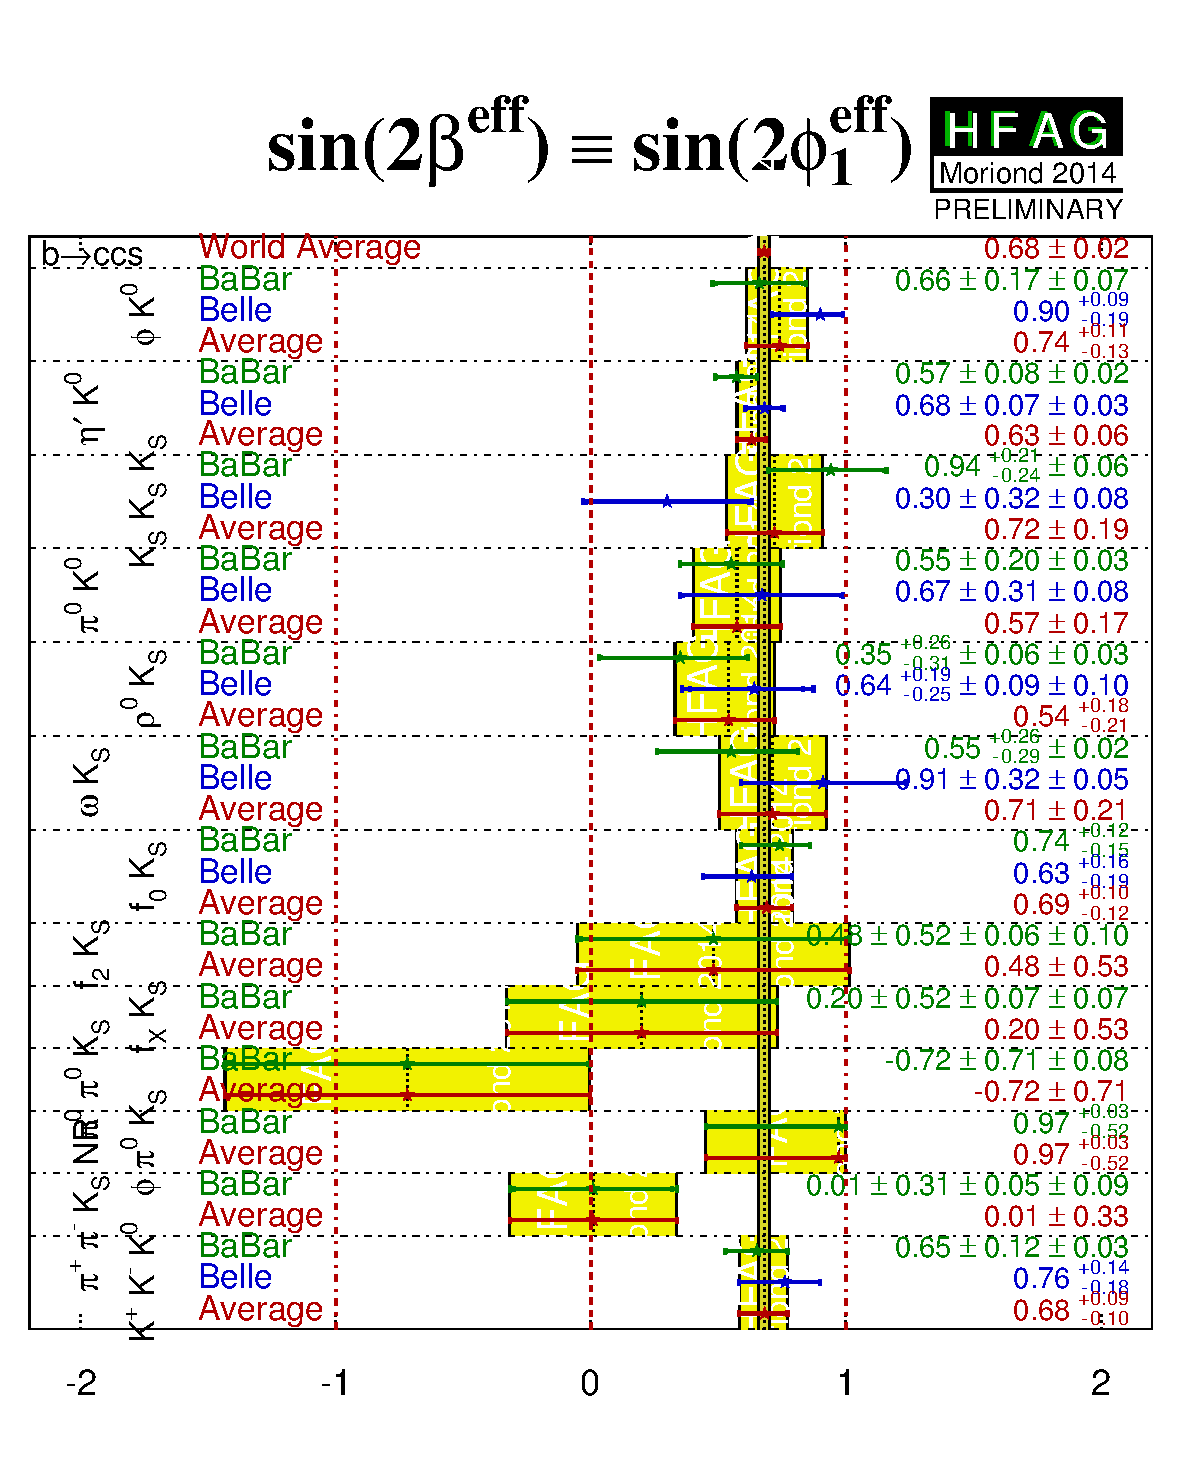
\includegraphics{figures/cp_uta/sPengS_CP}
    }
    \hfill
    \resizebox{0.45\textwidth}{!}{
      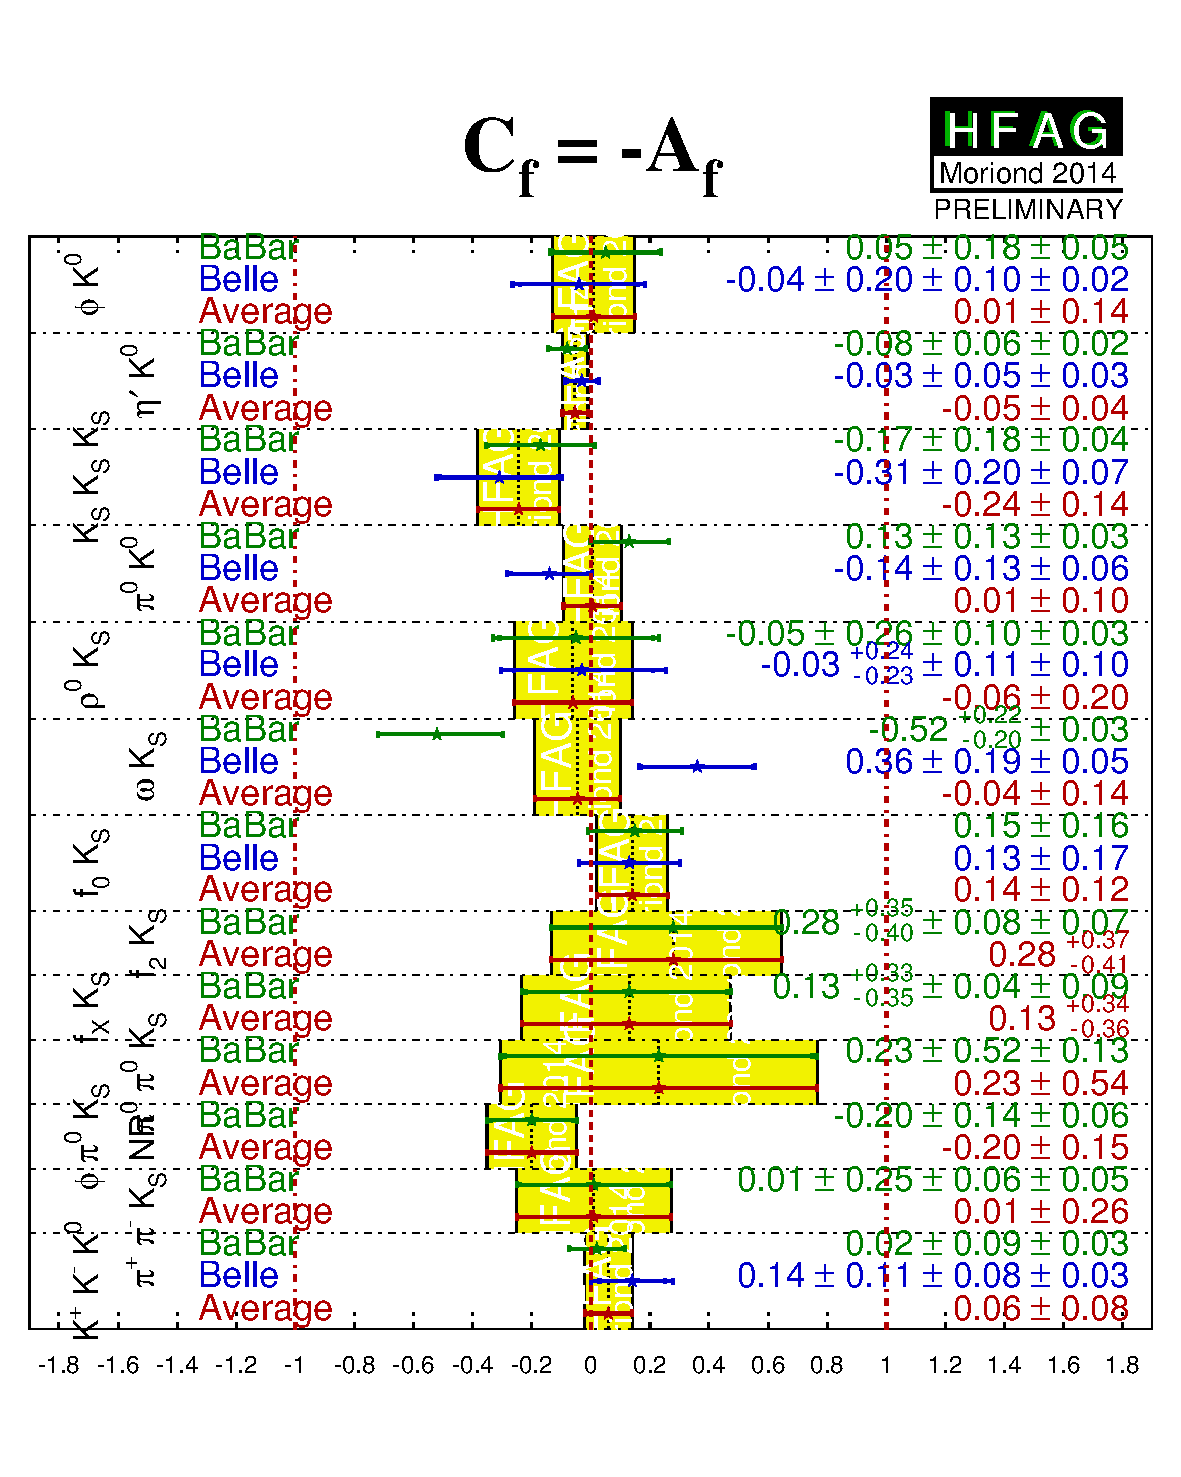
\includegraphics{figures/cp_uta/sPengC_CP}
    }
    \\
    \resizebox{0.45\textwidth}{!}{
      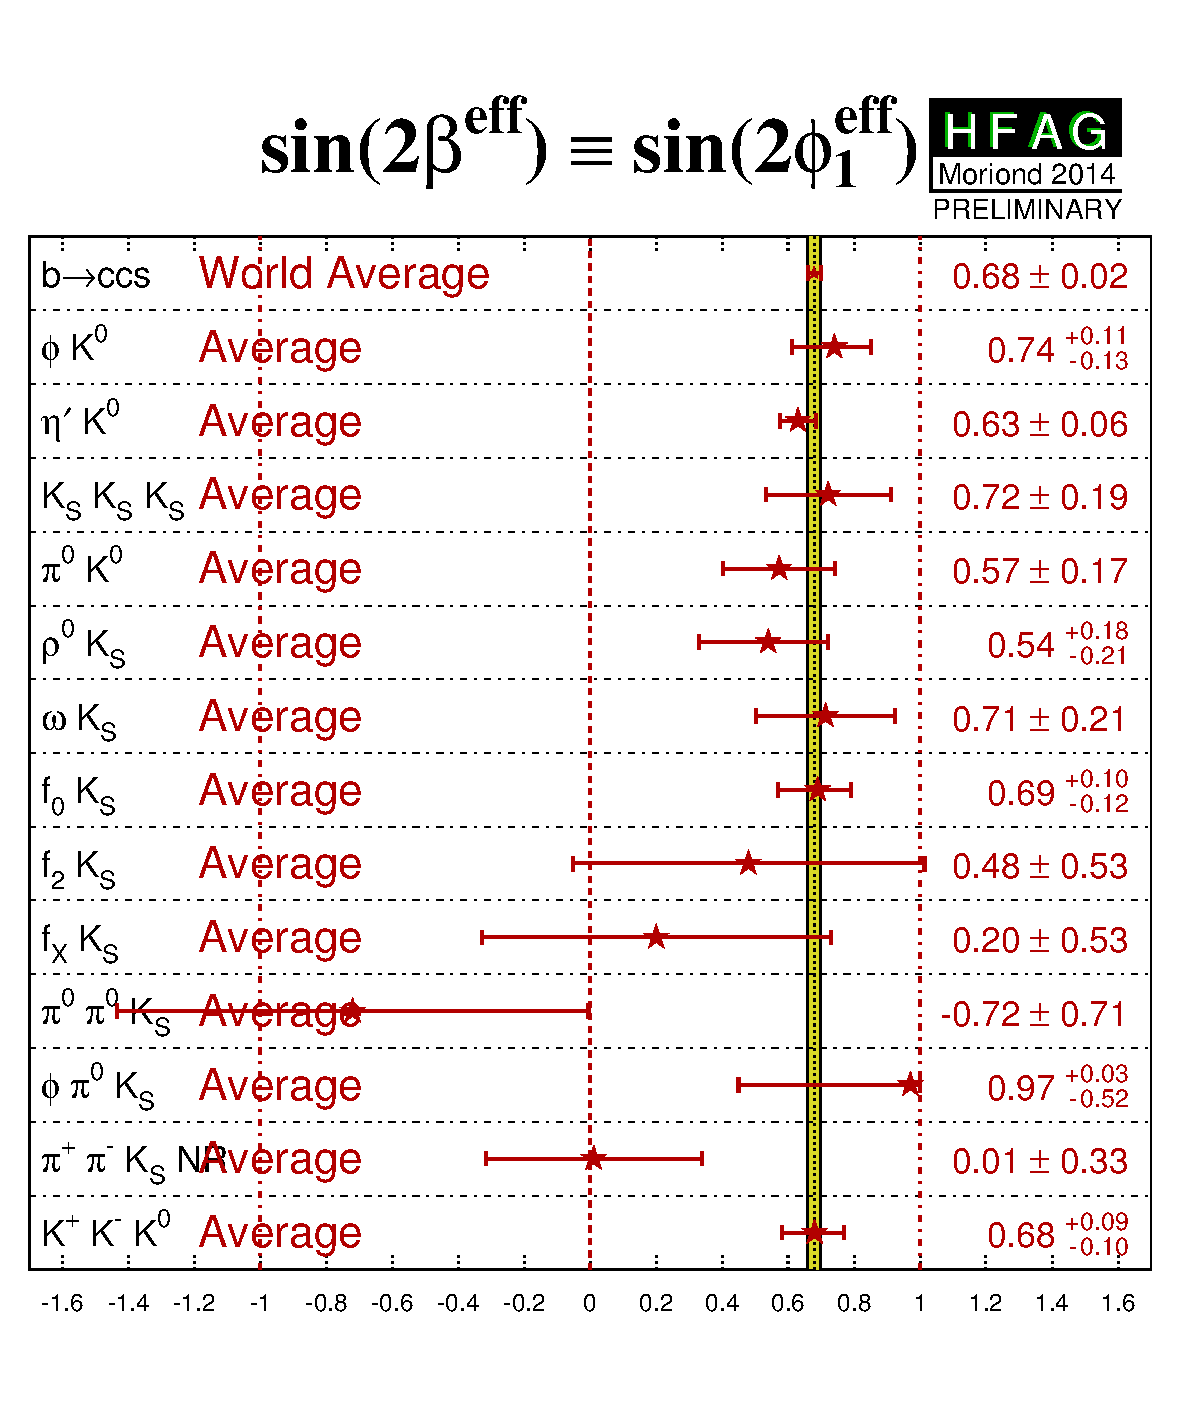
\includegraphics{figures/cp_uta/sPengS_CP_avOnly}
    }
    \hfill
    \resizebox{0.45\textwidth}{!}{
      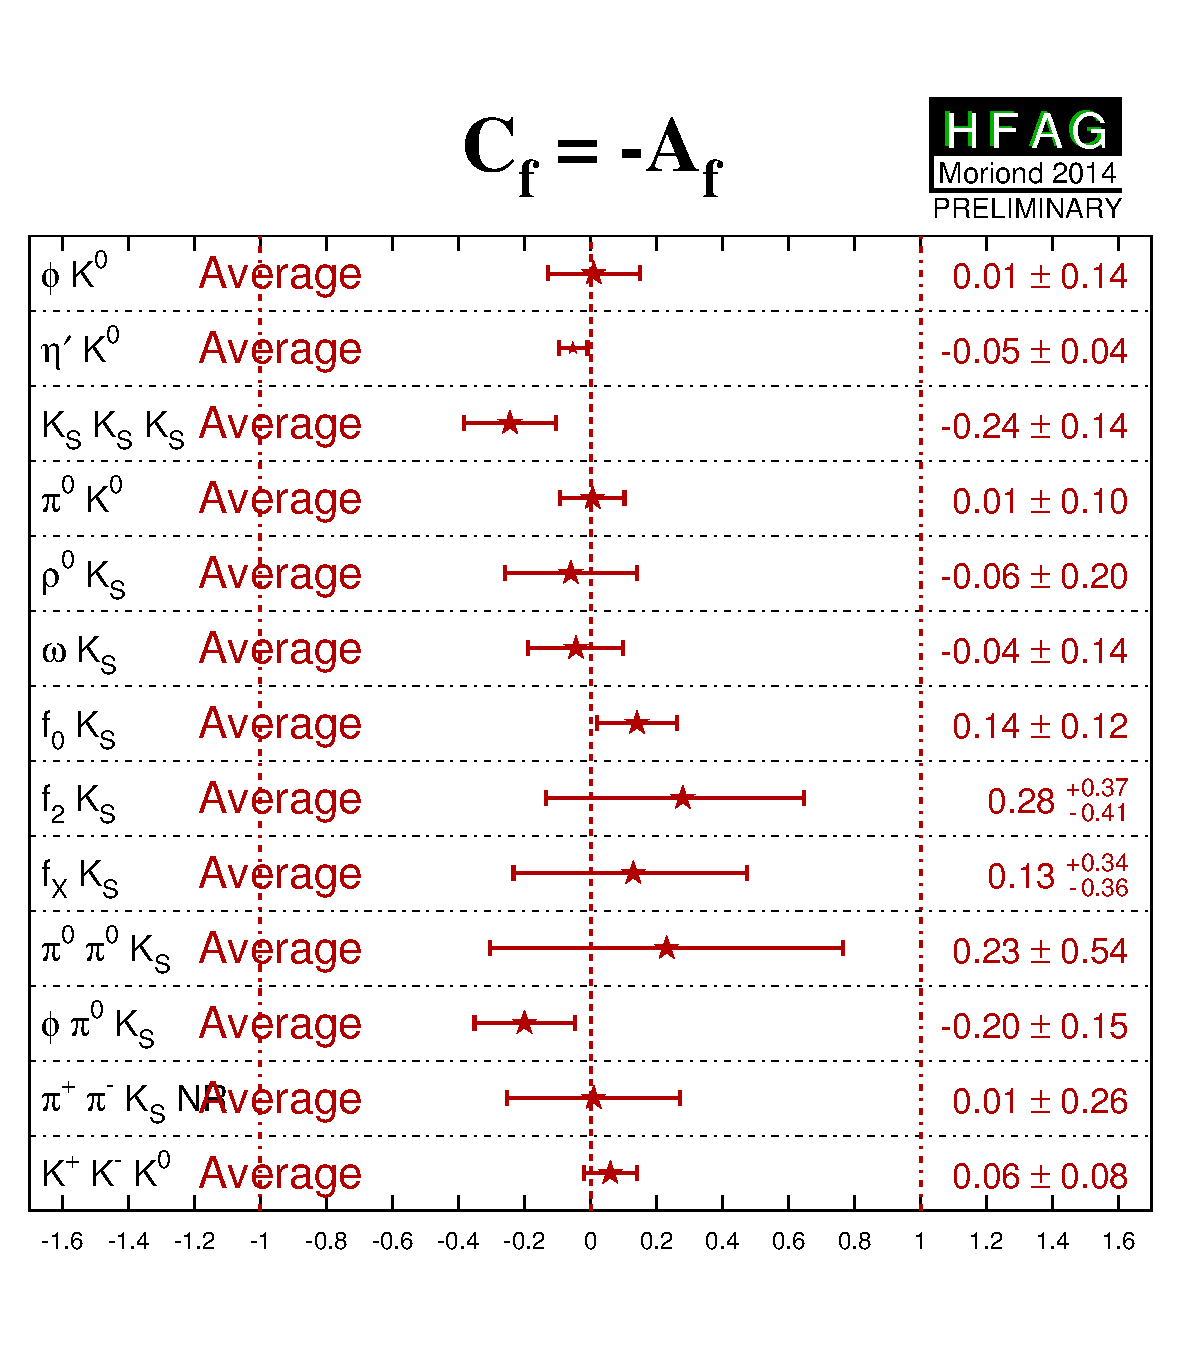
\includegraphics{figures/cp_uta/sPengC_CP_avOnly}
    }
  \end{center}
  \vspace{-0.8cm}
  \caption{
    (Top)
    Averages of 
    (left) $-\etacp S_{b \to q\bar q s}$ and (right) $C_{b \to q\bar q s}$.
    The $-\etacp S_{b \to q\bar q s}$ figure compares the results to 
    the world average 
    for $-\etacp S_{b \to c\bar c s}$ (see Section~\ref{sec:cp_uta:ccs:cp_eigen}).
    (Bottom) Same, but only averages for each mode are shown.
    More figures are available from the HFAG web pages.
  }
  \label{fig:cp_uta:qqs}
\end{figure}

\begin{figure}[htb]
  \begin{center}
    \resizebox{0.33\textwidth}{!}{
      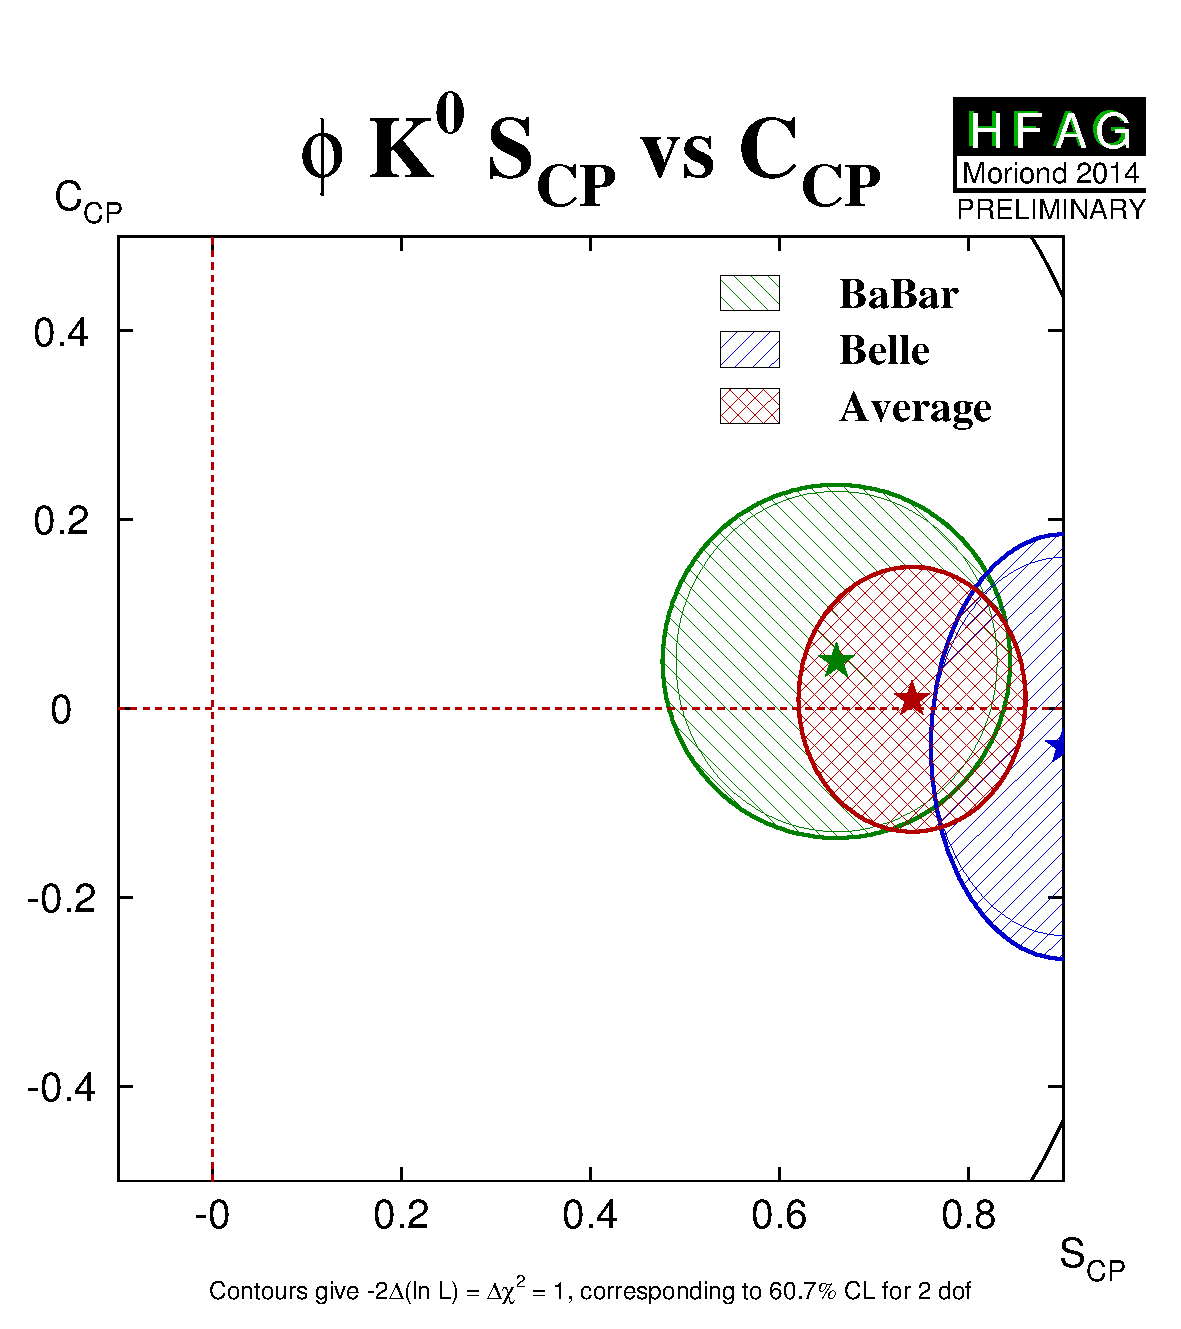
\includegraphics{figures/cp_uta/phiK0S_CPvsC_CP}
    }
    \hspace{0.08\textwidth}
    \resizebox{0.33\textwidth}{!}{
      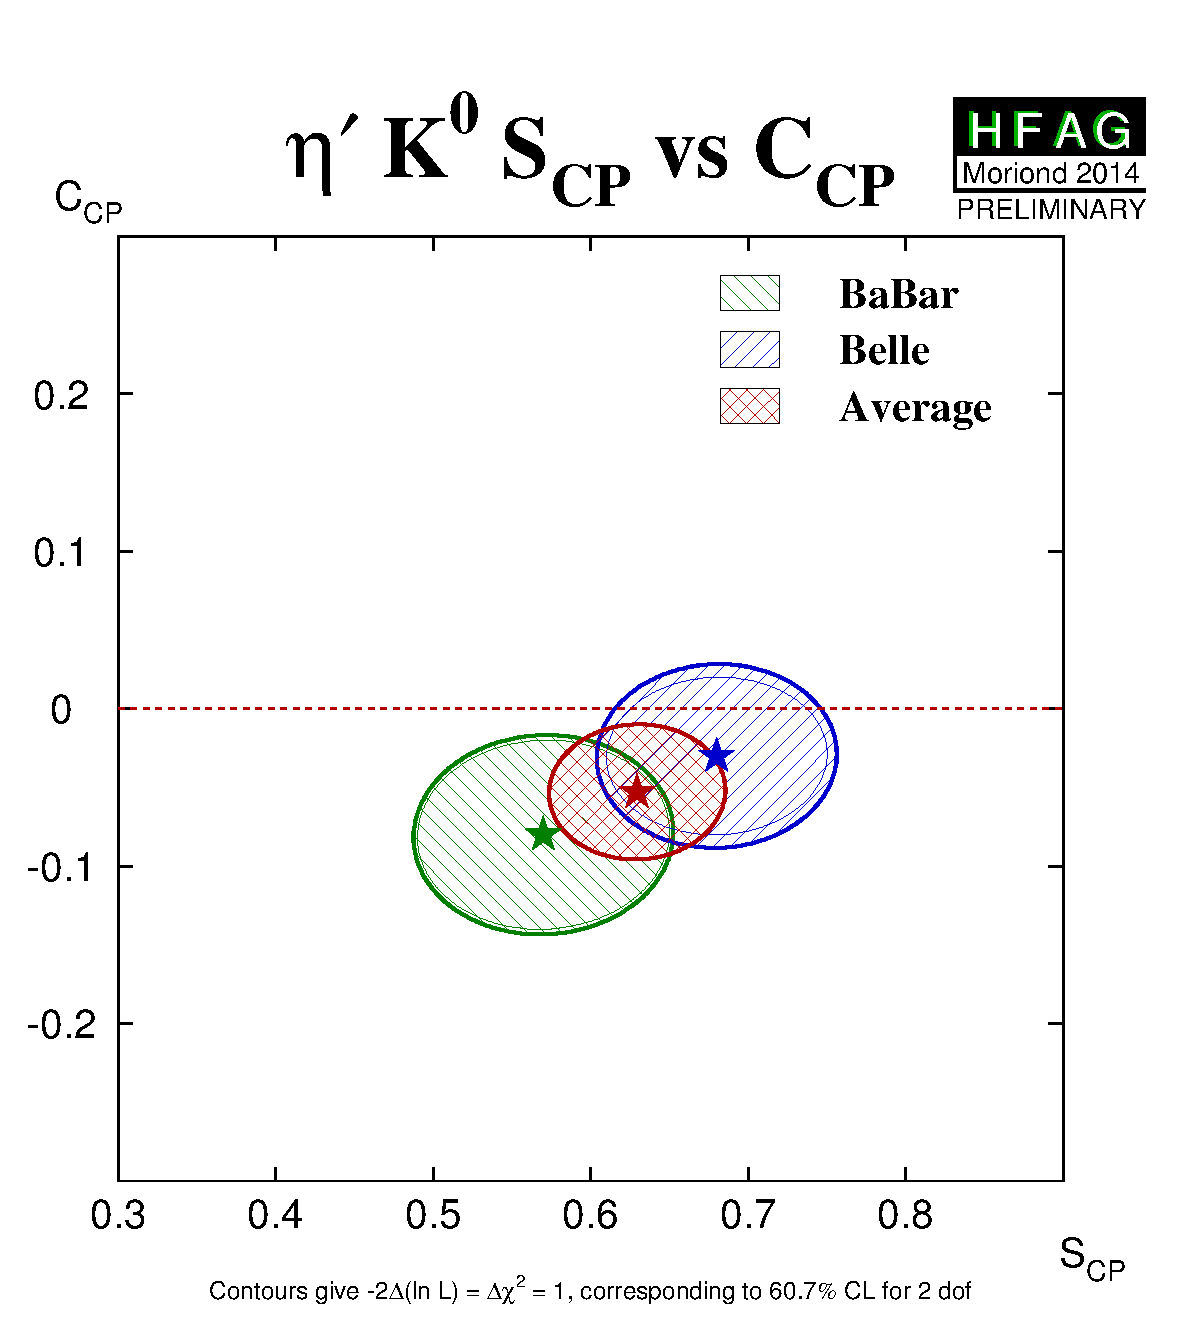
\includegraphics{figures/cp_uta/etaprimeK0S_CPvsC_CP}
    }
    \\
    \resizebox{0.33\textwidth}{!}{
      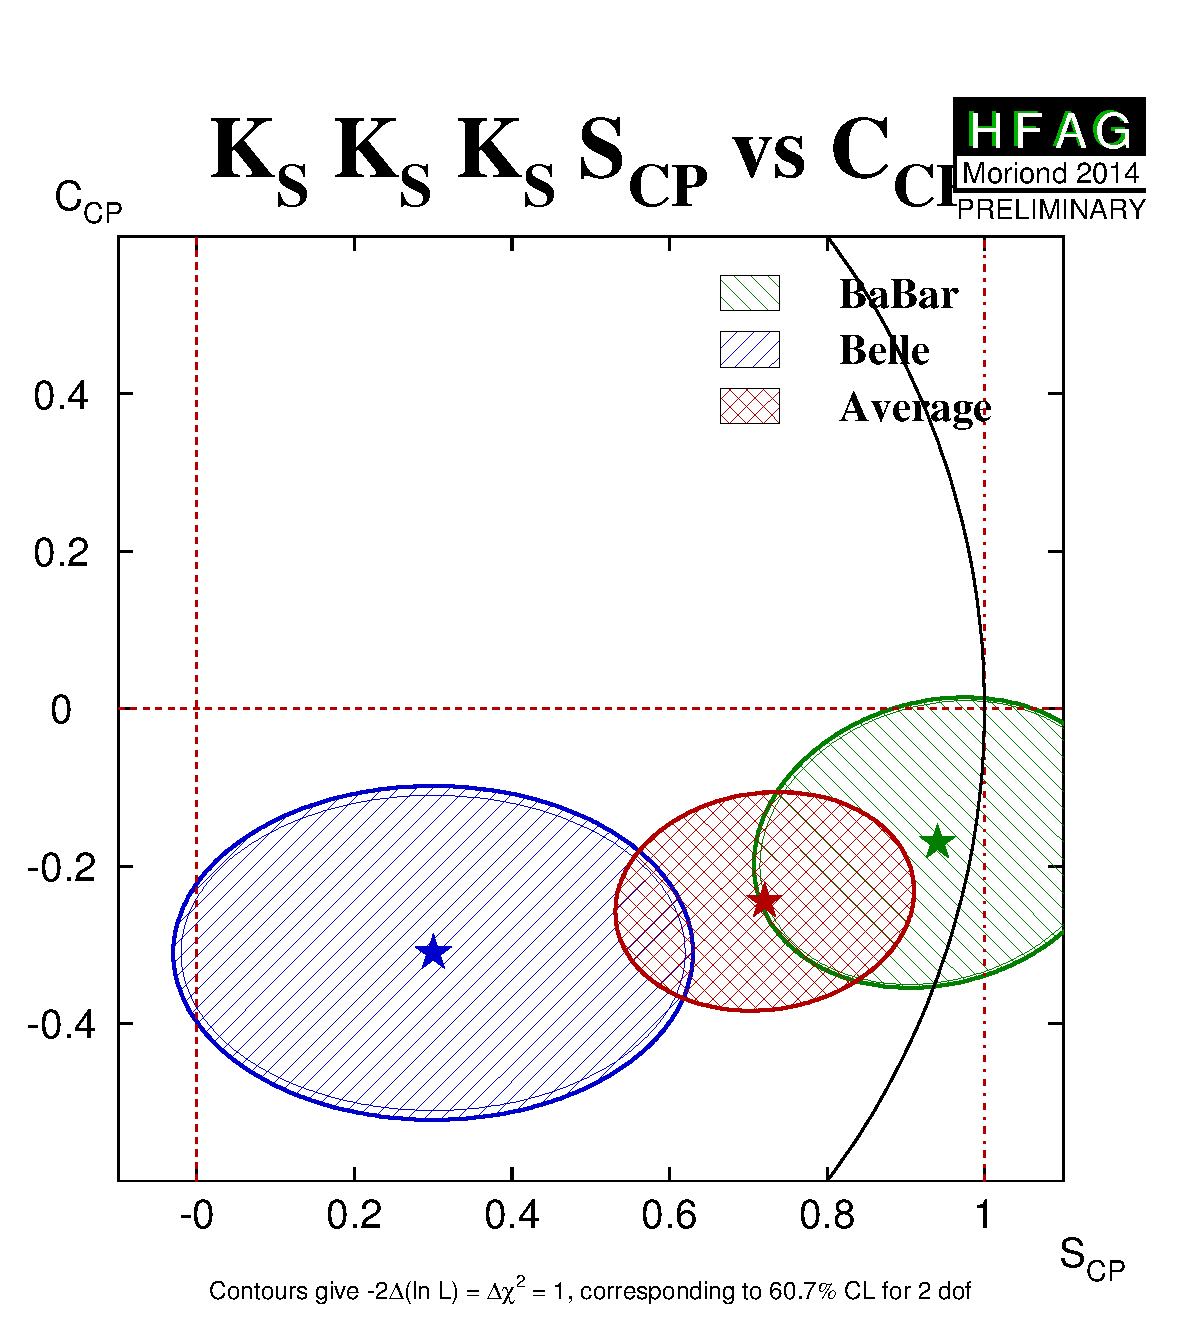
\includegraphics{figures/cp_uta/KSKSKSS_CPvsC_CP}
    }
    \hspace{0.08\textwidth}
    \resizebox{0.33\textwidth}{!}{
      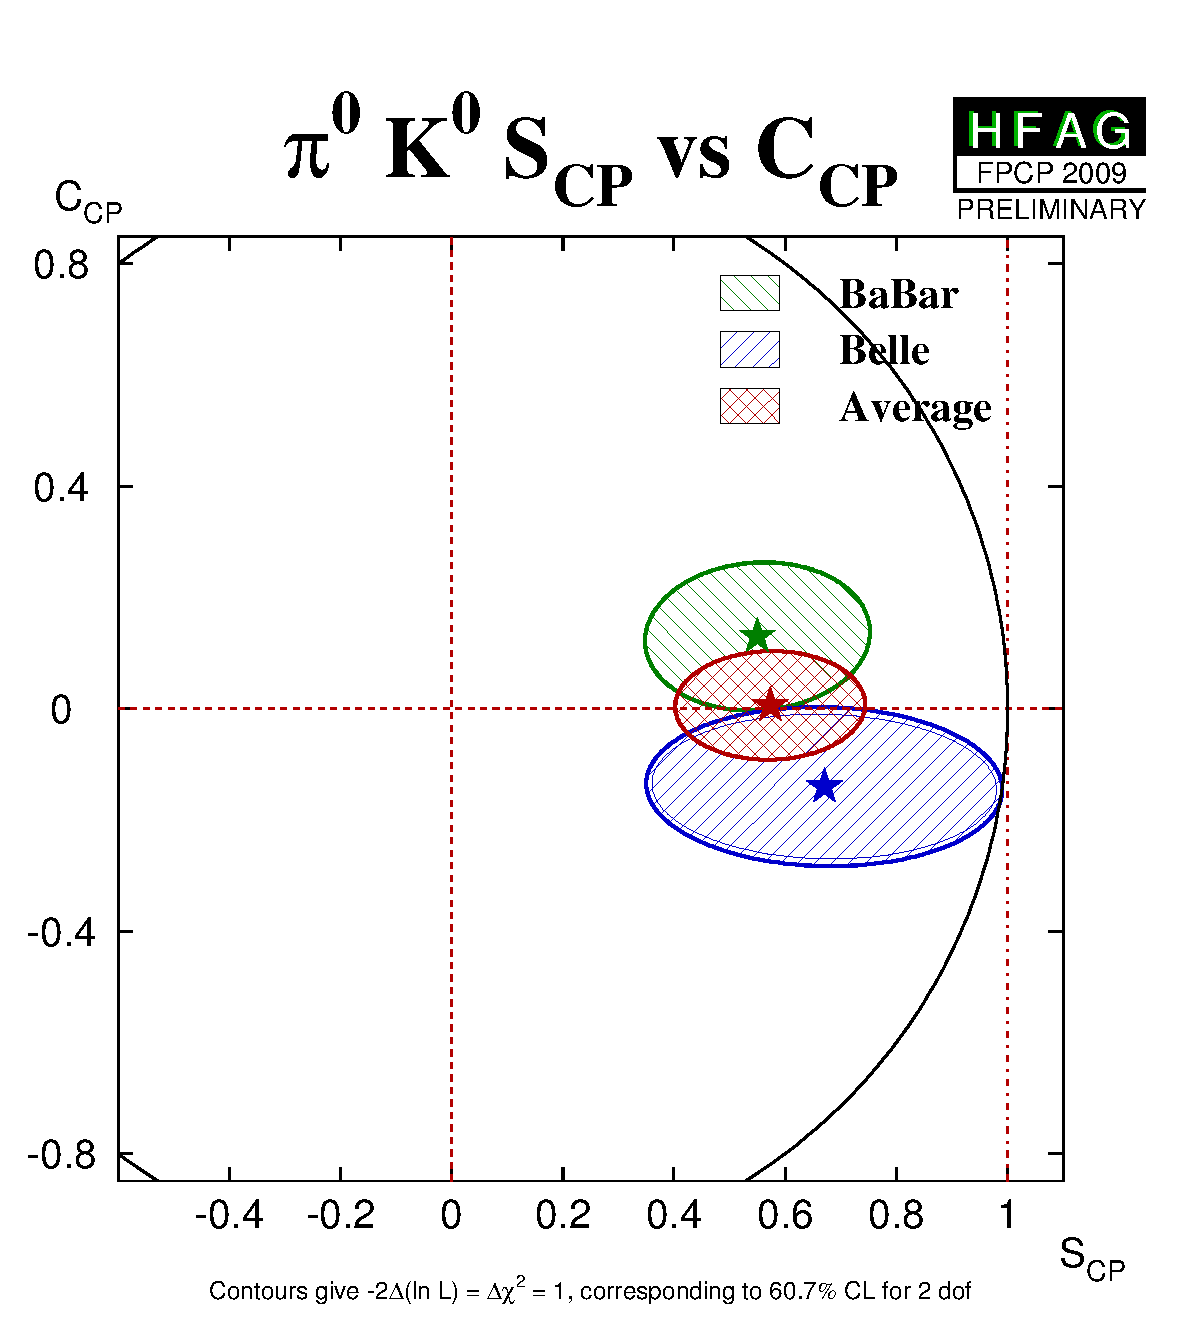
\includegraphics{figures/cp_uta/pi0K0S_CPvsC_CP}
    }
  \end{center}
  \vspace{-0.5cm}
  \caption{
    Averages of four $b \to q\bar q s$ dominated channels,
    for which correlated averages are performed,
    in the $S_{\CP}$ \vs\ $C_{\CP}$ plane,
    where $S_{\CP}$ has been corrected by the $\CP$ eigenvalue to give
    $\sin(2\beta^{\rm eff})$.
    (Top left) $\Bz \to \phi\Kz$,
    (top right) $\Bz \to \eta^\prime\Kz$,
    (bottom left) $\Bz \to \KS\KS\KS$,
    (bottom right) $\Bz \to \pi^0\KS$.
    More figures are available from the HFAG web pages.
  }
  \label{fig:cp_uta:qqs_SvsC}
\end{figure}

\begin{figure}[htb]
  \begin{center}
    \resizebox{0.66\textwidth}{!}{
      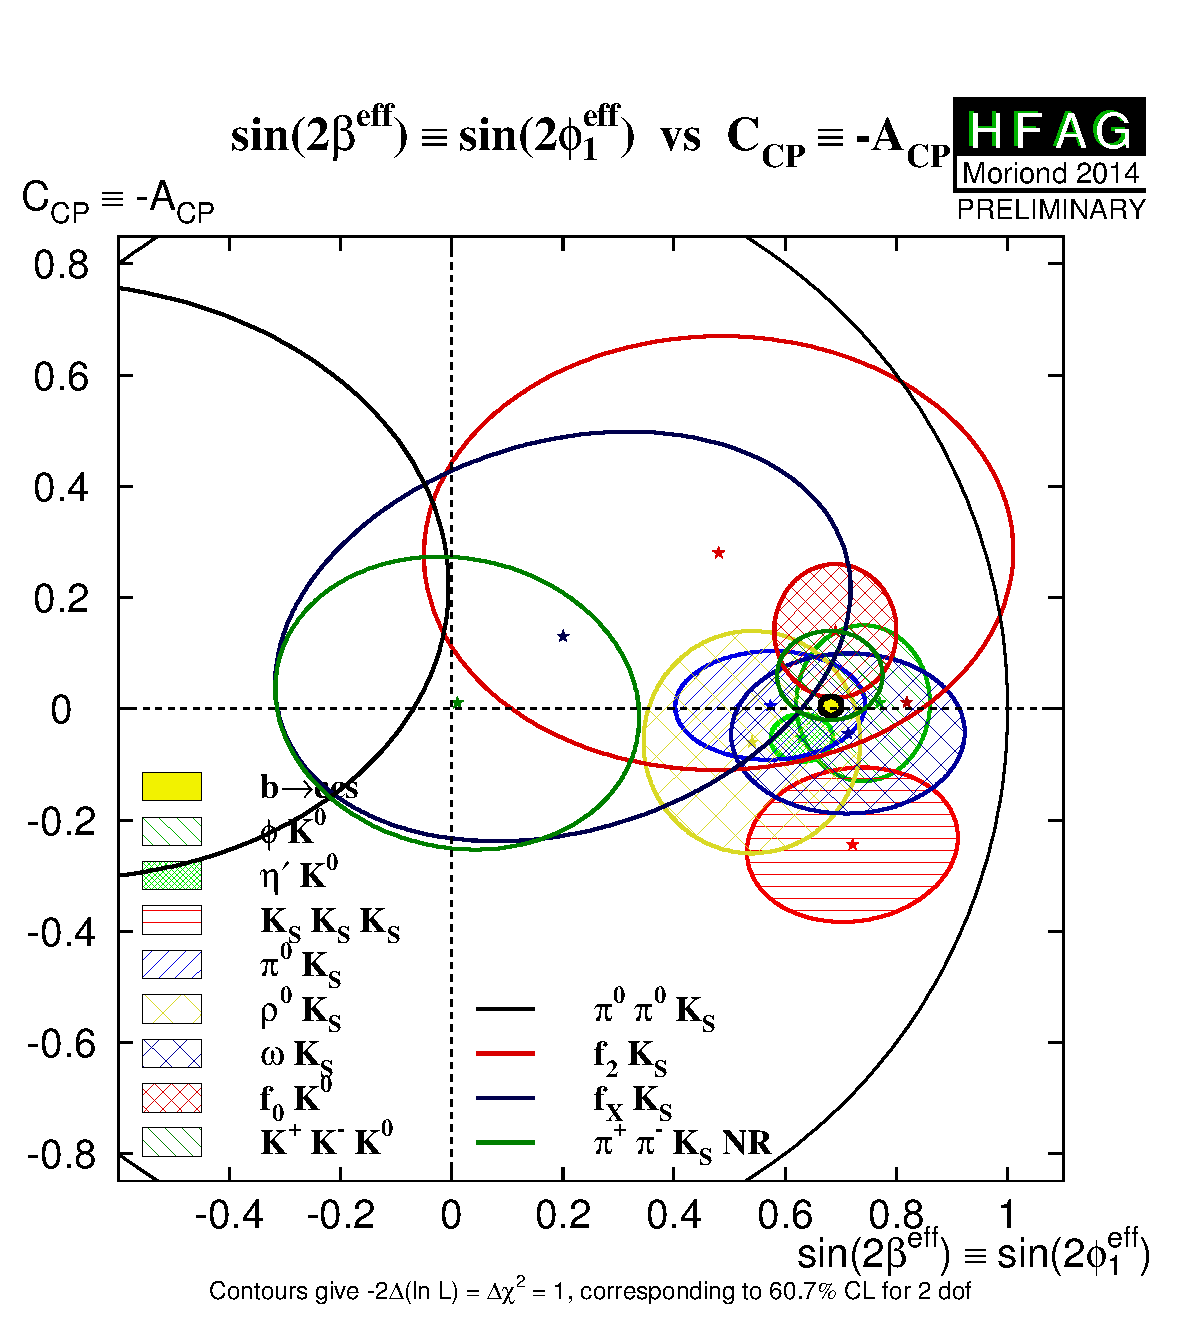
\includegraphics{figures/cp_uta//sPengS_CPvsC_CP}
    }
  \end{center}
  \vspace{-0.8cm}
  \caption{
    Compilation of constraints in the 
    $-\etacp S_{b \to q\bar q s}$ \vs\ $C_{b \to q\bar q s}$ plane.
  }
  \label{fig:cp_uta:qqs_SvsC-all}
\end{figure}

%% straightforward interpretation
As explained above,
each of the modes listed in Table~\ref{tab:cp_uta:qqs} has
different uncertainties within the Standard Model,
and so each may have a different value of $-\etacp S_{b \to q\bar q s}$.
Therefore, there is no strong motivation to make a combined average
over the different modes.
We refer to such an average as a ``na\"\i ve $s$-penguin average.''
It is na\"\i ve not only because of the neglect of the theoretical uncertainty,
but also since possible correlations of systematic effects 
between different modes are neglected.
In spite of these caveats, there remains substantial interest 
in the value of this quantity,
and therefore it is given here:
$\langle -\etacp S_{b \to q\bar q s} \rangle = 0.64 \pm 0.03$,
with confidence level $0.74~(0.3\sigma)$.
This value is in agreement with the average 
$-\etacp S_{b \to c\bar c s}$ given in Sec.~\ref{sec:cp_uta:ccs:cp_eigen}.
% However, this result is strongly effected by the highly non-Gaussian errors
% of the \babar\ result for 
% $\Bz \to f_0\Kz$ with $f_0 \to \pi^+\pi^-$~\cite{Aubert:2009me},
% which is only marginally consistent with \babar\ result for 
% $\Bz \to f_0\Kz$ with $f_0 \to K^+K^-$~\cite{Aubert:2007sd}
% and the \belle\ result for $\Bz \to f_0\Kz$ with $f_0 \to \pi^+\pi^-$ 
% (treated as a Q2B decay)~\cite{Abe:2006gy}.
% If the na\"\i ve $s$-penguin average is recalculated without this result,
% we find $\langle -\etacp S_{b \to q\bar q s} \rangle = 0.56 \pm 0.05$,
% with confidence level $0.25~(1.1\sigma)$.
% Again treating the uncertainties as Gaussian and neglecting correlations,
% this value is found to be $2.2\sigma$ below the average 
% $-\etacp S_{b \to c\bar c s}$ given in Sec.~\ref{sec:cp_uta:ccs:cp_eigen}.
%
(The average for $C_{b \to q\bar q s}$ is 
$\langle C_{b \to q\bar q s} \rangle = -0.01 \pm 0.03$
with confidence level $0.74~(0.3\sigma)$.)
% This result is not strongly effected by the inclusion of the \babar\ result for 
% $\Bz \to f_0\Kz$ with $f_0 \to \pi^+\pi^-$.)
%
We emphasise again that we do not advocate the use of these averages,
and that the values should be treated with {\it extreme caution}, if at all.
% What is unambiguous (although only qualitative) 
% is that there is a trend that the values 
% of $-\etacp S_{b \to q\bar q s}$ in different modes 
% are below the average for $-\etacp S_{b \to c\bar c s}$.

From Table~\ref{tab:cp_uta:qqs} it may be noted 
that the averages for $-\etacp S_{b \to q\bar q s}$ in 
$\phi\KS$, $\etapr \Kz$, $f_0\KS$ and $\Kp\Km\KS$
are all now more than $5\sigma$ away from zero, 
so that $\CP$ violation in these modes can be considered well established.
There is no evidence (above $2\sigma$) for $\CP$ violation in any $b \to q \bar q s$ decay.

%%%%%%%%
%%%
%%% qqs
%%%
%%%%%%%%
\mysubsubsection{Time-dependent Dalitz plot analyses: $\Bz \to K^+K^-\Kz$ and $\Bz \to \pi^+\pi^-\KS$}
\label{sec:cp_uta:qqs:dp}

As mentioned in Sec.~\ref{sec:cp_uta:notations:dalitz:kkk0} and above,
both \babar\ and \belle\ have performed time-dependent Dalitz plot analysis of
$\Bz \to K^+K^-\Kz$ and $\Bz \to \pi^+\pi^-\KS$ decays.
The results are summarised in Tables~\ref{tab:cp_uta:kkk0_tddp} 
and~\ref{tab:cp_uta:pipik0_tddp}.
Averages for the $\Bz\to f_0 \KS$ decay, which contributes to both Dalitz
plots, are shown in Fig.~\ref{fig:cp_uta:qqs:f0KS}.
Results are presented in terms of the effective weak phase (from mixing and
decay) difference $\beta^{\rm eff}$ and the parameter of $\CP$ violation in decay
$\Acp$ ($\Acp = -C$) for each of the resonant contributions.
Note that Dalitz plot analyses, including all those included in these
averages, often suffer from ambiguous solutions -- we quote the results
corresponding to those presented as solution 1 in all cases.
Results on flavour specific amplitudes that may contribute to these Dalitz
plots (such as $K^{*+}\pi^-$) are averaged by the HFAG Rare Decays subgroup 
(Sec.~\ref{sec:rare}).

% \begin{table}[htb]
\begin{sidewaystable}
  \begin{center}
    \caption{
      Results from time-dependent Dalitz plot analysis of 
      the $\Bz \to K^+K^-\Kz$ decay.
      Correlations (not shown) are taken into account in the average.
    }
    \vspace{0.2cm}
    \setlength{\tabcolsep}{0.0pc}
% make this tabular (not tabular*) and resize down to \textwidth
% change @{\extracolsep{\fill}} to @{\extracolsep{2mm}}
    \resizebox{\textwidth}{!}{
      \begin{tabular}{l@{\hspace{2mm}}r@{\hspace{2mm}}c@{\hspace{2mm}}|@{\hspace{2mm}}c@{\hspace{2mm}}c@{\hspace{2mm}}|@{\hspace{2mm}}c@{\hspace{2mm}}c|@{\hspace{2mm}}c@{\hspace{2mm}}c} 
        \hline 
        \mc{2}{l}{Experiment} & $N(B\bar{B})$ &
        \mc{2}{c}{$\phi\KS$} & \mc{2}{c}{$f_0\KS$} & \mc{2}{c}{$K^+K^-\KS$} \\
        & & & $\beta^{\rm eff}\,(^\circ)$ & $\Acp$ & $\beta^{\rm eff}\,(^\circ)$ & $\Acp$ & $\beta^{\rm eff}\,(^\circ)$ & $\Acp$ \\
	\babar & \cite{Lees:2012kx} & 470M & $21 \pm 6 \pm 2$ & $-0.05 \pm 0.18 \pm 0.05$ & $18 \pm 6 \pm 4$ & $-0.28 \pm 0.24 \pm 0.09$ & $20.3 \pm 4.3 \pm 1.2$ & $-0.02 \pm 0.09 \pm 0.03$ \\
	\belle & \cite{Nakahama:2010nj} & 657M & $32.2 \pm 9.0 \pm 2.6 \pm 1.4$ & $0.04 \pm 0.20 \pm 0.10 \pm 0.02$ & $31.3 \pm 9.0 \pm 3.4 \pm 4.0$ & $-0.30 \pm 0.29 \pm 0.11 \pm 0.09$ & $24.9 \pm 6.4 \pm 2.1 \pm 2.5$ & $-0.14 \pm 0.11 \pm 0.08 \pm 0.03$ \\
	\mc{2}{l}{\bf Average} & & $24 \pm 5$ & $-0.01 \pm 0.14$ & $22 \pm 6$ & $-0.29 \pm 0.20$ & $21.6 \pm 3.7$ & $-0.06 \pm 0.08$ \\
	\mc{3}{l}{\small Confidence level} & \mc{6}{c}{\small $0.93~(0.1\sigma)$} \\
        \hline
      \end{tabular}
    }
    
    \label{tab:cp_uta:kkk0_tddp}
  \end{center}
\end{sidewaystable}
% \end{table}

% \begin{table}[htb]
\begin{sidewaystable}
  \begin{center}
    \caption{
      Results from time-dependent Dalitz plot analysis of 
      the $\Bz \to \pi^+\pi^-\KS$ decay.
      Correlations (not shown) are taken into account in the average.
    }
    \vspace{0.2cm}
    \setlength{\tabcolsep}{0.0pc}
% make this tabular (not tabular*) and resize down to \textwidth
% change @{\extracolsep{\fill}} to @{\extracolsep{2mm}}
    \resizebox{\textwidth}{!}{
      \begin{tabular}{l@{\hspace{2mm}}r@{\hspace{2mm}}c@{\hspace{2mm}}|@{\hspace{2mm}}c@{\hspace{2mm}}c|@{\hspace{2mm}}c@{\hspace{2mm}}c} 
        \hline 
        \mc{2}{l}{Experiment} & $N(B\bar{B})$ & 
        \mc{2}{c}{$\rho^0\KS$} & \mc{2}{c}{$f_0\KS$} \\
        & & & $\beta^{\rm eff}$ & $\Acp$ & $\beta^{\rm eff}$ & $\Acp$ \\
        \hline
        \babar & \cite{Aubert:2009me} & 383M & $(10.2 \pm 8.9 \pm 3.0 \pm 1.9)^\circ$ & $0.05 \pm 0.26 \pm 0.10 \pm 0.03$ & $(36.0 \pm 9.8 \pm 2.1 \pm 2.1)^\circ$ & $-0.08 \pm 0.19 \pm 0.03 \pm 0.04$ \\
        \belle & \cite{:2008wwa} & 657M & $(20.0 \,^{+8.6}_{-8.5} \pm 3.2 \pm 3.5)^\circ$ & $0.03 \,^{+0.23}_{-0.24} \pm 0.11 \pm 0.10$ & $(12.7 \,^{+6.9}_{-6.5} \pm 2.8 \pm 3.3)^\circ$ & $-0.06 \pm 0.17 \pm 0.07 \pm 0.09$ \\
        \hline
        \mc{2}{l}{\bf Average} & & $16.4 \pm 6.8$ & $0.06 \pm 0.20$ & $20.6 \pm 6.2$ & $-0.07 \pm 0.14$  \\
        \mc{3}{l}{\small Confidence level} & \mc{4}{c}{\small $0.39~(0.9\sigma)$} \\
        \hline
      \end{tabular}
    }

    \vspace{2ex}

    \setlength{\tabcolsep}{0.0pc}
% make this tabular (not tabular*) and resize down to \textwidth
% change @{\extracolsep{\fill}} to @{\extracolsep{2mm}}
    \resizebox{\textwidth}{!}{
      \begin{tabular}{l@{\hspace{2mm}}r@{\hspace{2mm}}c@{\hspace{2mm}}|@{\hspace{2mm}}c@{\hspace{2mm}}c|@{\hspace{2mm}}c@{\hspace{2mm}}c} 
        \hline 
        \mc{2}{l}{Experiment} & $N(B\bar{B})$ & 
        \mc{2}{c}{$f_2\KS$} & \mc{2}{c}{$f_{\rm X}\KS$} \\
        & & & $\beta^{\rm eff}$ & $\Acp$ & $\beta^{\rm eff}$ & $\Acp$ \\
        \babar & \cite{Aubert:2009me} & 383M & $(14.9 \pm 17.9 \pm 3.1 \pm 5.2)^\circ$ & $-0.28 \,^{+0.40}_{-0.35} \pm 0.08 \pm 0.07$ & $(5.8 \pm 15.2 \pm 2.2 \pm 2.3)^\circ$ & $-0.13 \,^{+0.35}_{-0.33} \pm 0.04 \pm 0.09$ \\
        \hline
      \end{tabular}
    }

    \vspace{2ex}

    \setlength{\tabcolsep}{0.0pc}
% make this tabular (not tabular*) and resize down to \textwidth
% change @{\extracolsep{\fill}} to @{\extracolsep{2mm}}
    \resizebox{\textwidth}{!}{
      \begin{tabular}{l@{\hspace{2mm}}r@{\hspace{2mm}}c@{\hspace{2mm}}|@{\hspace{2mm}}c@{\hspace{2mm}}c|@{\hspace{2mm}}c@{\hspace{2mm}}c} 
        \hline 
        \mc{2}{l}{Experiment} & $N(B\bar{B})$ & 
        \mc{2}{c}{$\Bz \to \pi^+\pi^-\KS$ nonresonant} & \mc{2}{c}{$\chi_{c0}\KS$} \\
        & & & $\beta^{\rm eff}$ & $\Acp$ & $\beta^{\rm eff}$ & $\Acp$ \\
        \babar & \cite{Aubert:2009me} & 383M & $(0.4 \pm 8.8 \pm 1.9 \pm 3.8)^\circ$ & $-0.01 \pm 0.25 \pm 0.06 \pm 0.05$ & $(23.2 \pm 22.4 \pm 2.3 \pm 4.2)^\circ$ & $0.29 \,^{+0.44}_{-0.53} \pm 0.03 \pm 0.05$ \\
        \hline
      \end{tabular}
    }

    \label{tab:cp_uta:pipik0_tddp}
  \end{center}
\end{sidewaystable}
% \end{table}



%% From the results in Table~\ref{tab:cp_uta:pipik0_tddp},
%% \babar\ infer that the trigonometric reflection 
%% at $\pi/2 - \beta^{\rm eff}$ in $\Bz \to K^+K^-\Kz$,
%% which is inconsistent with the Standard Model expectation,
%% is disfavoured at $4.8\sigma$.

\begin{figure}[htb]
  \begin{center}
    \resizebox{0.45\textwidth}{!}{
      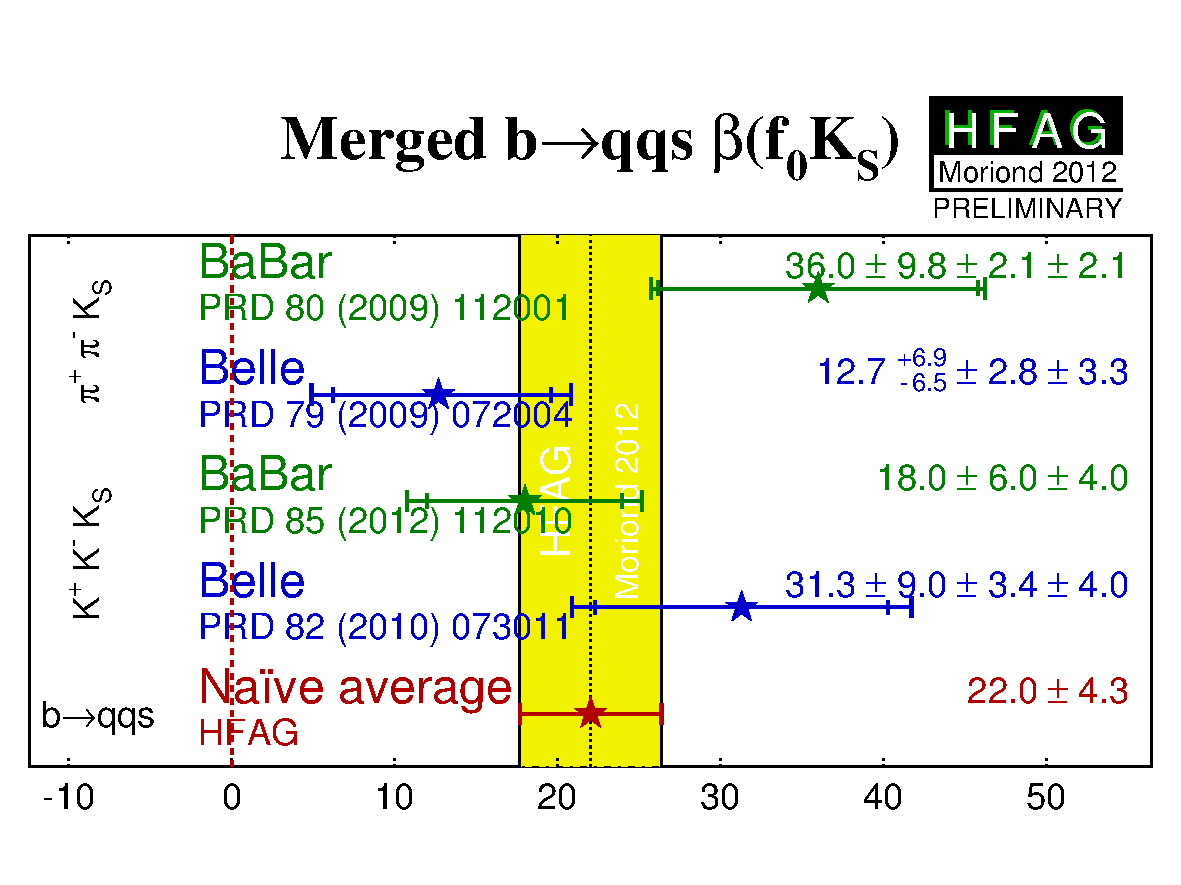
\includegraphics{figures/cp_uta/f0KSbeta}
    }
    \hfill
    \resizebox{0.45\textwidth}{!}{
      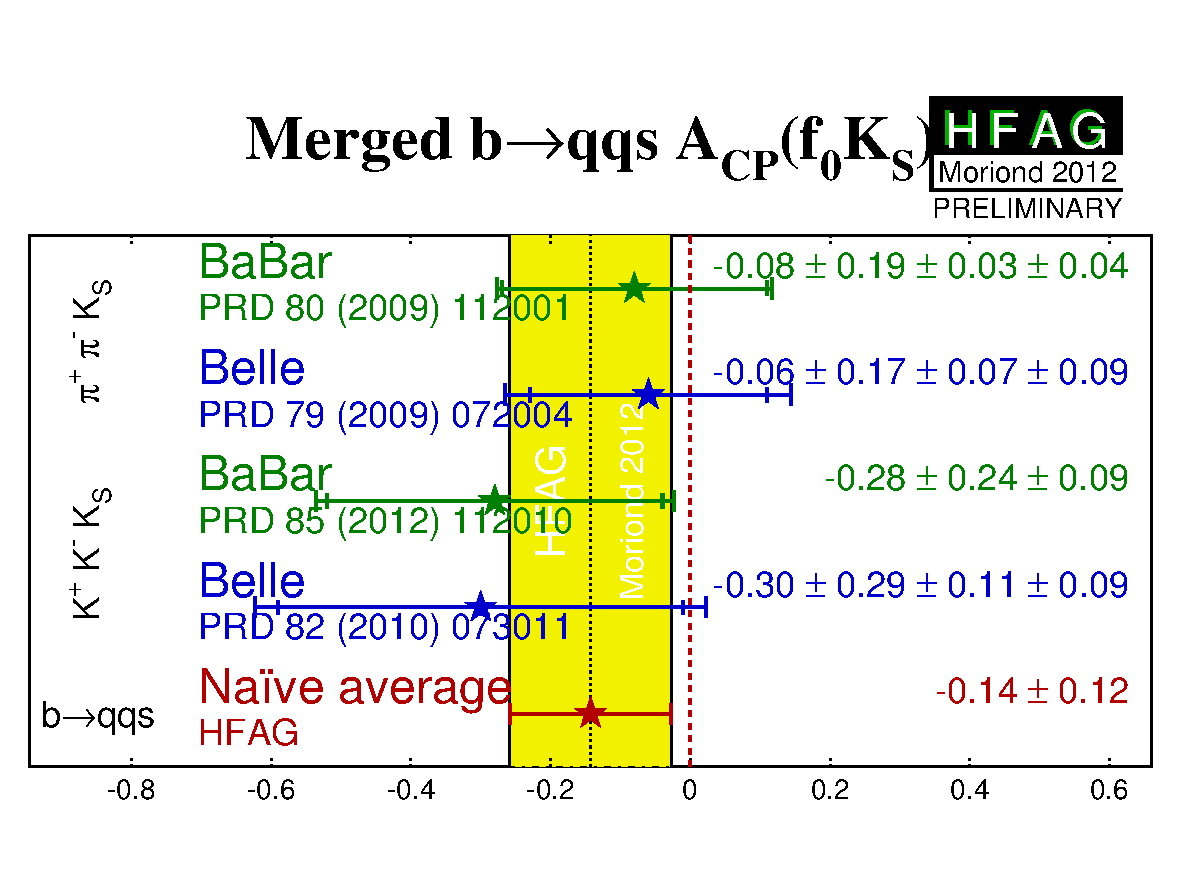
\includegraphics{figures/cp_uta/f0KSA_CP}
    }
  \end{center}
  \vspace{-0.8cm}
  \caption{
    Averages of 
    (left) $\beta^{\rm eff} \equiv \phi_1^{\rm eff}$ and (right) $A_{\CP}$
    for the $\Bz\to f_0\KS$ decay including measurements from Dalitz plot analyses of both $\Bz\to K^+K^-\KS$ and $\Bz\to \pi^+\pi^-\KS$.
  }
  \label{fig:cp_uta:qqs:f0KS}
\end{figure}

%%%%%%%%
%%%
%%% qqs
%%%
%%%%%%%%
\mysubsubsection{Time-dependent analyses of $\Bz \to \phi \KS \pi^0$}
\label{sec:cp_uta:qqs:vv}

The final state in the decay $\Bz \to \phi \KS \pi^0$ is a mixture of \CP-even
and \CP-odd amplitudes. However, since only $\phi K^{*0}$ resonant states
contribute (in particular, $\phi K^{*0}(892)$, $\phi K^{*0}_0(1430)$ and $\phi
K^{*0}_2(1430)$ are seen), the composition can be determined from the analysis
of $B \to \phi K^+ \pi^-$, assuming only that the ratio of branching fractions
${\cal B}(K^{*0} \to \KS \pi^0)/{\cal B}(K^{*0} \to K^+ \pi^-)$ is the same
for each exited kaon state. 

\babar~\cite{Aubert:2008zza} have performed a simultaneous analysis of 
$\Bz \to \phi \KS \pi^0$ and $\Bz \to \phi K^+ \pi^-$ that is time-dependent
for the former mode and time-integrated for the latter. Such an analysis
allows, in principle, all parameters of the $\Bz \to \phi K^{*0}$ system to be
determined, including mixing-induced \CP violation effects. The latter is
determined to be $\Delta\phi_{00} = 0.28 \pm 0.42 \pm 0.04$, where
$\Delta\phi_{00}$ is half the weak phase difference between $\Bz$ and $\Bzb$
decays to $\phi K^{*0}_0(1430)$. As discussed above, this can also be
presented in terms of the quasi-two-body parameter $\sin(2\beta^{\rm eff}_{00}) =
\sin(2\beta+2\Delta\phi_{00}) = 0.97 \,^{+0.03}_{-0.52}$. The highly asymmetric
uncertainty arises due to the conversion from the phase to the sine of the
phase, and the proximity of the physical boundary. 

Similar $\sin(2\beta^{\rm eff})$ parameters can be defined for each of the
helicity amplitudes for both $\phi K^{*0}(892)$ and $\phi
K^{*0}_2(1430)$. However, the relative phases between these decays are
constrained due to the nature of the simultaneous analysis of $\Bz \to \phi
\KS \pi^0$ and $\Bz \to \phi K^+ \pi^-$, and therefore these measurements are
highly correlated. Instead of quoting all these results, \babar provide an
illustration of their measurements with the following differences: 
\begin{eqnarray}
  \sin(2\beta - 2\Delta\delta_{01}) - \sin(2\beta) & = & -0.42\,^{+0.26}_{-0.34} \, \\
  \sin(2\beta - 2\Delta\phi_{\parallel1}) - \sin(2\beta) & = & -0.32\,^{+0.22}_{-0.30} \, \\
  \sin(2\beta - 2\Delta\phi_{\perp1}) - \sin(2\beta) & = & -0.30\,^{+0.23}_{-0.32} \, \\
  \sin(2\beta - 2\Delta\phi_{\perp1}) - \sin(2\beta - 2\Delta\phi_{\parallel1})
  & = & 0.02 \pm 0.23 \, \\
  \sin(2\beta - 2\Delta\delta_{02}) - \sin(2\beta) & = & -0.10\,^{+0.18}_{-0.29} \,
\end{eqnarray}
where the first subscript indicates the helicity amplitude and the second
indicates the spin of the kaon resonance. For the complete definitions of the
$\Delta\delta$ and $\Delta\phi$ parameters, please refer to the \babar\ paper~\cite{Aubert:2008zza}.

Parameters of \CP violation in decay for each of the contributing helicity
amplitudes can also be measured. Again, these are determined from a
simultaneous fit of $\Bz \to \phi \KS \pi^0$ and $\Bz \to \phi K^+ \pi^-$,
with the precision being dominated by the statistics of the latter mode. 
Direct \CP violation measurements are tabulated by HFAG - Rare Decays (Sec.~\ref{sec:rare}). 

%%%%%%%%
%%%
%%% qqs
%%%
%%%%%%%%
\mysubsubsection{Time-dependent \CP asymmetries in $\Bs \to \Kp\Km$}
\label{sec:cp_uta:qqs:BstoKK}

The decay $\Bs \to \Kp\Km$ involves a $b \to u\bar{u}s$ transition, and hence has both penguin and tree contributions. Both mixing-induced and \CP violation in decay effects may arise, and additional input is needed to disentangle the contributions and determine $\gamma$ and $\beta_s^{\rm eff}$. For example, the observables in $\Bd \to \pip\pim$ can be related using U-spin, as proposed by Fleischer~\cite{Fleischer:1999pa}.

The observables are $A_{\rm mix} = S_{\CP}$, $A_{\rm dir} = -C_{\CP}$, and $A_{\Delta\Gamma}$. They can all be treated as free parameters, but are physically constrained to satisfy $A_{\rm mix}^2 + A_{\rm dir}^2 + A_{\Delta\Gamma}^2 = 1$. Note that the untagged decay distribution, from which an ``effective lifetime'' can be measured, retains sensitivity to $A_{\Delta\Gamma}$. Averages of effective lifetimes are performed by the HFAG Lifetimes and Oscillations group, see Sec.~\ref{sec:life_mix}.

The observables in $\Bs \to \Kp\Km$ have been measured by LHCb, who impose the constraint mentioned above to eliminate $A_{\rm \Delta\Gamma}$. 

\begin{table}[!htb]
	\begin{center}
		\caption{
      Results from time-dependent analysis of the $\Bs \to K^{+} K^{-}$ decay.
		}
		\vspace{0.2cm}
		\setlength{\tabcolsep}{0.0pc}
		\begin{tabular*}{\textwidth}{@{\extracolsep{\fill}}lrcccc} \hline
	\mc{2}{l}{Experiment} & Sample size & $A_{\rm mix}$ & $A_{\rm dir}$ & Correlation \\
	\hline
	LHCb & \cite{Aaij:2013tna} & $1.0 \ {\rm fb}^{-1}$ & $0.30 \pm 0.12 \pm 0.04$ & $0.14 \pm 0.11 \pm 0.03$ & 0.02 \\
	\hline
%	\mc{3}{l}{\bf Average} & $0.17 \pm 0.19$ & $0.02 \pm 0.18$ & {\small uncorrelated averages} \\
%	\mc{3}{l}{\small Confidence level} & {\small $0.xx~(y.y\sigma)$} & {\small $0.xx~(y.y\sigma)$} & \\
%		\hline
		\end{tabular*}
		\label{tab:cp_uta:BstoKK}
	\end{center}
\end{table}




\mysubsubsection{Time-dependent \CP asymmetries in $\Bs \to \phi\phi$}
\label{sec:cp_uta:qqs:Bstophiphi}

 The decay $\Bs \to \phi\phi$ involves a $b \to s\bar{s}s$ transition, and hence is a ``pure penguin'' mode (in the limit that the $\phi$ meson is treated as a pure $s\bar{s}$ state). Since the mixing phase and the decay phase are expected to cancel in the Standard Model, the prediction for the phase from the interference of mixing and decay is predicted to be $\phi_s(\phi\phi) = 0$ with low uncertainty~\cite{Raidal:2002ph}. Due to the vector-vector nature of the final state, angular analysis is needed to separate the \CP-even and \CP-odd contributions. Such an analysis also makes it possible to fit directly for $\phi_s(\phi\phi)$.

A constraint on $\phi_s(\phi\phi)$ has been obtained by LHCb using $3.0 \,{\rm fb}^{-1}$ of data~\cite{Aaij:2014kxa}.
The result is $\phi_s(\phi\phi) = -0.17 \pm 0.15 \pm 0.03 \, {\rm rad}$ where the first uncertainty is statistical and the second is systematic. 


%%%%%%%%
%%%
%%% ccd
%%%
%%%%%%%%
\clearpage
\mysubsection{Time-dependent $\CP$ asymmetries in $b \to c\bar{c}d$ transitions
}
\label{sec:cp_uta:ccd}

The transition $b \to c\bar c d$ can occur via either a $b \to c$ tree
or a $b \to d$ penguin amplitude.  
Similarly to Eq.~(\ref{eq:cp_uta:b_to_s}), the amplitude for 
the $b \to d$ penguin can be written
\begin{equation}
  \label{eq:cp_uta:b_to_d}
  \begin{array}{ccccc}
    A_{b \to d} & = & 
    \mc{3}{l}{F_u V_{ub}V^*_{ud} + F_c V_{cb}V^*_{cd} + F_t V_{tb}V^*_{td}} \\
    & = & (F_u - F_c) V_{ub}V^*_{ud} & + & (F_t - F_c) V_{tb}V^*_{td} \\
    & = & {\cal O}(\lambda^3) & + & {\cal O}(\lambda^3). \\
  \end{array}
\end{equation}
From this it can be seen that the $b \to d$ penguin amplitude 
contains terms with different weak phases at the same order of
CKM suppression.

In the above, we have followed Eq.~(\ref{eq:cp_uta:b_to_s}) 
by eliminating the $F_c$ term using unitarity.
However, we could equally well write
\begin{equation}
  \label{eq:cp_uta:b_to_d_alt}
  \begin{array}{ccccc}
    A_{b \to d} 
    & = & (F_u - F_t) V_{ub}V^*_{ud} & + & (F_c - F_t) V_{cb}V^*_{cd}, \\
    & = & (F_c - F_u) V_{cb}V^*_{cd} & + & (F_t - F_u) V_{tb}V^*_{td}. \\
  \end{array}
\end{equation}
Since the $b \to c\bar{c}d$ tree amplitude 
has the weak phase of $V_{cb}V^*_{cd}$,
either of the above expressions allow the penguin to be decomposed into 
parts with weak phases the same and different to the tree amplitude
(the relative weak phase can be chosen to be either $\beta$ or $\gamma$).
However, if the tree amplitude dominates,
there is little sensitivity to any phase 
other than that from $\Bz$\textendash$\Bzb$ mixing.

The $b \to c\bar{c}d$ transitions can be investigated with studies 
of various different final states. 
Results are available from both \babar\  and \belle\ 
using the final states $\jpsi \pi^0$, $D^+D^-$, 
$D^{*+}D^{*-}$ and $D^{*\pm}D^{\mp}$,
the averages of these results are given in Tables~\ref{tab:cp_uta:ccd1} and~\ref{tab:cp_uta:ccd2}.
The results using the $\CP$ eigenstate ($\etacp = +1$) modes
$\jpsi \pi^0$ and $D^+D^-$
are shown in Fig.~\ref{fig:cp_uta:ccd:psipi0} and 
Fig.~\ref{fig:cp_uta:ccd:dd} respectively,
with two-dimensional constraints shown in Fig.~\ref{fig:cp_uta:ccd_SvsC}.

The vector-vector mode $D^{*+}D^{*-}$ 
is found to be dominated by the $\CP$-even longitudinally polarised component;
\babar\ measures a $\CP$-odd fraction of 
$0.158 \pm 0.028 \pm 0.006$~\cite{Aubert:2008ah} while
\belle\ measures a $\CP$-odd fraction of 
$0.125 \pm 0.043 \pm 0.023$~\cite{:2009za}.
These values, listed as $R_\perp$, are included in the averages which ensures
the correlations to be taken into account.\footnote{
  Note that the \babar\ value given in Table~\ref{tab:cp_uta:ccd2} differs from
  that given above, since that in the table is not corrected for efficiency.
}
\babar\ have also performed an additional fit in which the 
$\CP$-even and $\CP$-odd components are allowed to have different 
$\CP$ violation parameters $S$ and $C$.  
These results are included in Table~\ref{tab:cp_uta:ccd2}.
Results using $D^{*+}D^{*-}$ are shown in Fig.~\ref{fig:cp_uta:ccd:dstardstar}.

%% For the non-$\CP$ eigenstate mode $D^{*\pm}D^{\mp}$
%% \babar\ uses fully reconstructed events while 
%% \belle\ combines both fully and partially reconstructed samples.
%% At present we perform uncorrelated averages of the parameters in the 
%% $D^{*\pm}D^{\mp}$ system.

As discussed in Sec.~\ref{sec:cp_uta:notations:non_cp}, the most recent papers on the non-$\CP$ eigenstate mode $D^{*\pm}D^{\mp}$ use the ($A$, $S$, $\Delta S$, $C$, $\Delta C$) set of parameters, and we therefore perform the averages with this choice.

\begin{table}[htb]
	\begin{center}
		\caption{
     Averages for the $b \to c\bar{c}d$ modes,
     $\Bz \to J/\psi \pi^{0}$ and $D^+D^-$.
%			Averages for $J/\psi \pi^{0}$.
		}
		\vspace{0.2cm}
		\setlength{\tabcolsep}{0.0pc}
		\begin{tabular*}{\textwidth}{@{\extracolsep{\fill}}lrcccc} \hline
	\mc{2}{l}{Experiment} & $N(B\bar{B})$ & $S_{CP}$ & $C_{CP}$ & Correlation \\
	\hline
        \mc{6}{c}{$J/\psi \pi^{0}$} \\
	\babar & \cite{Aubert:2008bs} & 466M & $-1.23 \pm 0.21 \pm 0.04$ & $-0.20 \pm 0.19 \pm 0.03$ & $0.20$ \\
	\belle & \cite{:2007wd} & 535M & $-0.65 \pm 0.21 \pm 0.05$ & $-0.08 \pm 0.16 \pm 0.05$ & $-0.10$ \\
%	\hline
	\mc{3}{l}{\bf Average} & $-0.93 \pm 0.15$ & $-0.10 \pm 0.13$ & $0.04$ \\
	\mc{3}{l}{\small Confidence level} & \mc{2}{c}{\small $0.15~(1.4\sigma)$} & \\
		\hline
% 		\end{tabular*}
% 		\label{tab:cp_uta:yyy}
% 	\end{center}
% \end{table}

% \begin{table}[htb]
% 	\begin{center}
% 		\caption{
% 			Averages for $D^{+} D^{-}$.
% 		}
% 		\vspace{0.2cm}
% 		\setlength{\tabcolsep}{0.0pc}
%		\begin{tabular*}{\textwidth}{@{\extracolsep{\fill}}lrcccc} \hline
% 		\mc{2}{l}{Experiment} & $N(B\bar{B})$ & $S_{CP}$ & $C_{CP}$ & Correlation \\
% 		\hline
        \mc{6}{c}{$D^{+} D^{-}$} \\
	\babar & \cite{Aubert:2008ah} & 467M & $-0.65 \pm 0.36 \pm 0.05$ & $-0.07 \pm 0.23 \pm 0.03$ & $-0.01$ \\
	\belle & \cite{Rohrken:2012ta} & 772M & $-1.06 \,^{+0.21}_{-0.14} \pm 0.08$ & $-0.43 \pm 0.16 \pm 0.05$ & $-0.12$ \\
%	\hline
	\mc{3}{l}{\bf Average} & $-0.98 \pm 0.17$ & $-0.31 \pm 0.14$ & $-0.08$ \\
	\mc{3}{l}{\small Confidence level} & \mc{2}{c}{\small $0.26~(1.1\sigma)$} & \\
		\hline
 		\end{tabular*}
 		\label{tab:cp_uta:ccd1}
 	\end{center}
 \end{table}

% \begin{table}[htb]
\begin{sidewaystable}
 	\begin{center}
 		\caption{
      Averages for the $b \to c\bar{c}d$ modes,
      $D^{*+} D^{*-}$ and $D^{*\pm}D^\mp$.
 		}
% 		\vspace{0.2cm}
% 		\setlength{\tabcolsep}{0.0pc}

 		\begin{tabular*}{\textwidth}{@{\extracolsep{\fill}}lrcccc} \hline
 		\mc{2}{l}{Experiment} & $N(B\bar{B})$ & $S_{CP}$ & $C_{CP}$ & $R_\perp$ \\
 		\hline
        \mc{6}{c}{$D^{*+} D^{*-}$} \\
	\babar & \cite{Aubert:2008ah} & 467M & $-0.70 \pm 0.16 \pm 0.03$ & $0.05 \pm 0.09 \pm 0.02$ & $0.17 \pm 0.03$ \\
	\babar part. rec. & \cite{Lees:2012px} & 471M & $-0.49 \pm 0.18 \pm 0.07 \pm 0.04$ & $0.15 \pm 0.09 \pm 0.04$ & $0.15 \pm 10.00$ \\
	\belle & \cite{Kronenbitter:2012ha} & 772M & $-0.79 \pm 0.13 \pm 0.03$ & $-0.15 \pm 0.08 \pm 0.02$ & $0.14 \pm 0.02 \pm 0.01$ \\
%	\hline
	\mc{3}{l}{\bf Average} & $-0.71 \pm 0.09$ & $-0.01 \pm 0.05$ & $0.15 \pm 0.02$ \\
	\mc{3}{l}{\small Confidence level} & \mc{3}{c}{\small $0.72~(0.4\sigma)$} \\
		\hline
		\end{tabular*}
% 		\label{tab:cp_uta:yyy}
% 	\end{center}
% \end{table}

                \vspace{2ex}

%\begin{table}[htb]
% 	\begin{center}
% 		\caption{
% 			Averages for $D*^{+} D*^{-} 2$.
% 		}
% 		\vspace{0.2cm}
% 		\setlength{\tabcolsep}{0.0pc}
% make this tabular (not tabular*) and resize down to \textwidth
% change @{\extracolsep{\fill}} to @{\extracolsep{2mm}}
    \resizebox{\textwidth}{!}{
		\begin{tabular}{@{\extracolsep{2mm}}lrcccccc} \hline
	\mc{2}{l}{Experiment} & $N(B\bar{B})$ & $S_{CP+}$ & $C_{CP+}$ & $S_{CP-}$ & $C_{CP-}$ & $R_\perp$ \\
	\hline
        \mc{7}{c}{$D^{*+} D^{*-}$} \\
	\babar & \cite{Aubert:2008ah} & 467M & $-0.76 \pm 0.16 \pm 0.04$ & $0.02 \pm 0.12 \pm 0.02$ & $-1.81 \pm 0.71 \pm 0.16$ & $0.41 \pm 0.50 \pm 0.08$ & $0.15 \pm 0.03$ \\
%	\hline
%	\mc{3}{l}{\bf Average} & $-0.76 \pm 0.16$ & $0.02 \pm 0.12$ & $-1.81 \pm 0.73$ & $0.41 \pm 0.51$ & $0.15 \pm 0.03$ & \textendash{} \\
%	\mc{3}{l}{\small Confidence level} & \mc{5}{c}{\small $0.xx~(y.y\sigma)$} & \\
		\hline
		\end{tabular}
    }
% 		\label{tab:cp_uta:yyy}
% 	\end{center}
% \end{table}

                \vspace{2ex}

% \begin{table}[htb]
% 	\begin{center}
% 		\caption{
% 			Averages for $D*^{\pm} D^{\mp}$.
% 		}
% 		\vspace{0.2cm}
% 		\setlength{\tabcolsep}{0.0pc}
% make this tabular (not tabular*) and resize down to \textwidth
% change @{\extracolsep{\fill}} to @{\extracolsep{2mm}}
    \resizebox{\textwidth}{!}{
		\begin{tabular}{@{\extracolsep{2mm}}lrcccccc} \hline
	\mc{2}{l}{Experiment} & $N(B\bar{B})$ & $S$ & $C$ & $\Delta S$ & $\Delta C$ & ${\cal A}$ \\
        \hline
        \mc{8}{c}{$D^{*\pm} D^{\mp}$} \\
	\babar & \cite{Aubert:2008ah} & 467M & $-0.68 \pm 0.15 \pm 0.04$ & $0.04 \pm 0.12 \pm 0.03$ & $0.05 \pm 0.15 \pm 0.02$ & $0.04 \pm 0.12 \pm 0.03$ & $0.01 \pm 0.05 \pm 0.01$ \\
	\belle & \cite{Rohrken:2012ta} & 772M & $-0.78 \pm 0.15 \pm 0.05$ & $-0.01 \pm 0.11 \pm 0.04$ & $-0.13 \pm 0.15 \pm 0.04$ & $0.12 \pm 0.11 \pm 0.03$ & $0.06 \pm 0.05 \pm 0.02$ \\
%	\hline
	\mc{3}{l}{\bf Average} & $-0.73 \pm 0.11$ & $0.01 \pm 0.09$ & $-0.04 \pm 0.11$ & $0.08 \pm 0.08$ & $0.03 \pm 0.04$ \\
	\mc{3}{l}{\small Confidence level} & {\small $0.65~(0.5\sigma)$} & {\small $0.77~(0.3\sigma)$} & {\small $0.41~(0.8\sigma)$} & {\small $0.63~(0.5\sigma)$} & {\small $0.48~(0.7\sigma)$} \\
        \hline
                \end{tabular}
    }
		\label{tab:cp_uta:ccd2}
	\end{center}
\end{sidewaystable}
% \end{table}


In the absence of the penguin contribution (tree dominance),
the time-dependent parameters would be given by
$S_{b \to c\bar c d} = - \etacp \sin(2\beta)$,
$C_{b \to c\bar c d} = 0$,
$S_{+-} = \sin(2\beta + \delta)$,
$S_{-+} = \sin(2\beta - \delta)$,
$C_{+-} = - C_{-+}$ and 
${\cal A} = 0$,
where $\delta$ is the strong phase difference between the 
$D^{*+}D^-$ and $D^{*-}D^+$ decay amplitudes.
In the presence of the penguin contribution,
there is no clean interpretation in terms of CKM parameters,
however
direct $\CP$ violation may be observed as any of
$C_{b \to c\bar c d} \neq 0$, $C_{+-} \neq - C_{-+}$ or $A_{+-} \neq 0$.

The averages for the $b \to c\bar c d$ modes 
are shown in Figs.~\ref{fig:cp_uta:ccd} and~\ref{fig:cp_uta:ccd_SvsC-all}.
Results are consistent with tree dominance,
and with the Standard Model,
though the \belle\ results in $\Bz \to D^+D^-$~\cite{Fratina:2007zk}
show an indication of $\CP$ violation in decay,
and hence a non-zero penguin contribution.
The average of $S_{b \to c\bar c d}$ in both $J/\psi \pi^{0}$ and
$D^{*+}D^{*-}$ final states is more than $5\sigma$ from zero, corresponding to
observations of \CP violation in these decay channels.,
That in the $D^+D^-$ final state is more than $3\sigma$ from zero;
however, due to the large uncertainty and possible non-Gaussian effects,
any strong conclusion should be deferred.

% Comparisons of the results for the $b \to c\bar c d$ modes 
% to the $b \to c\bar c s$ and $b \to q\bar q s$ modes,
% can be seen in Fig.~\ref{fig:cp_uta:qqs_ccd}.

\begin{figure}[htb]
  \begin{center}
    \begin{tabular}{cc}
      \resizebox{0.46\textwidth}{!}{
        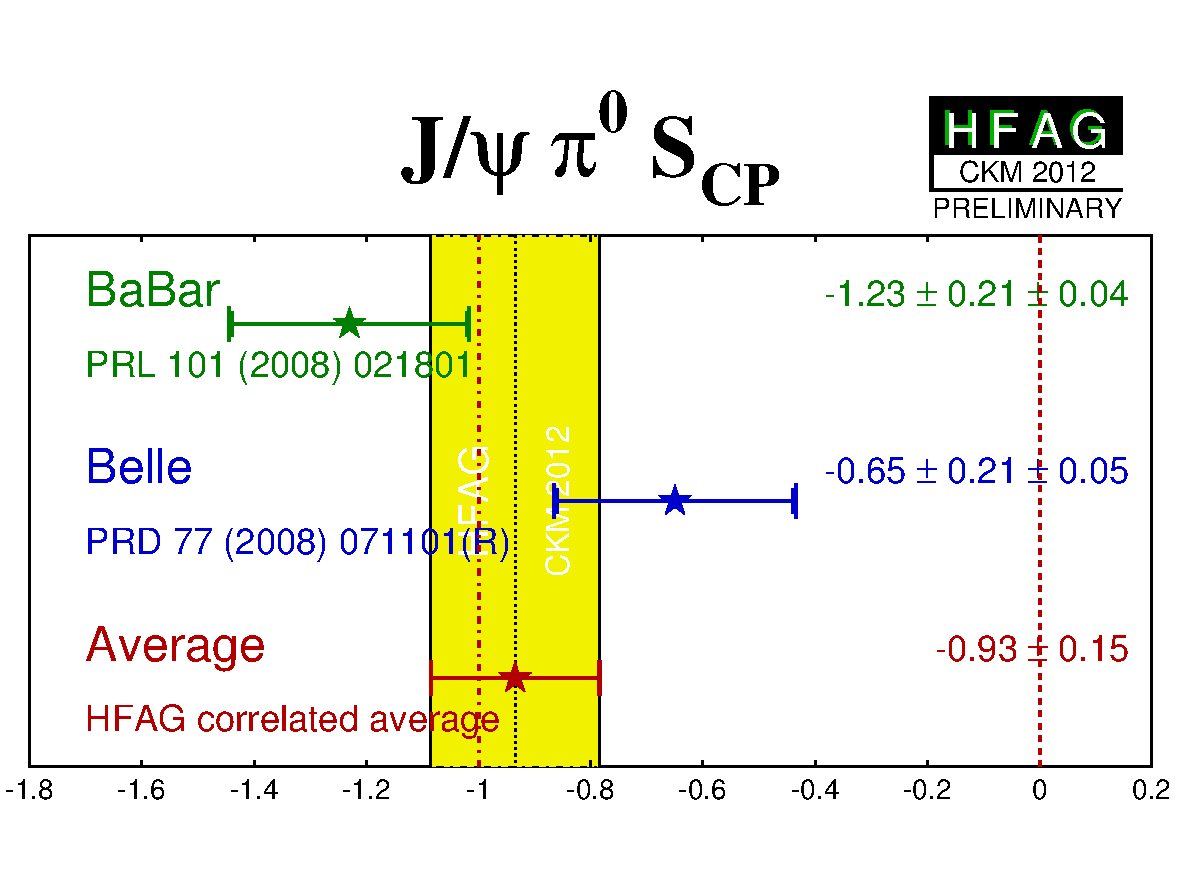
\includegraphics{figures/cp_uta/Jpsipi0S_CP}
      }
      &
      \resizebox{0.46\textwidth}{!}{
        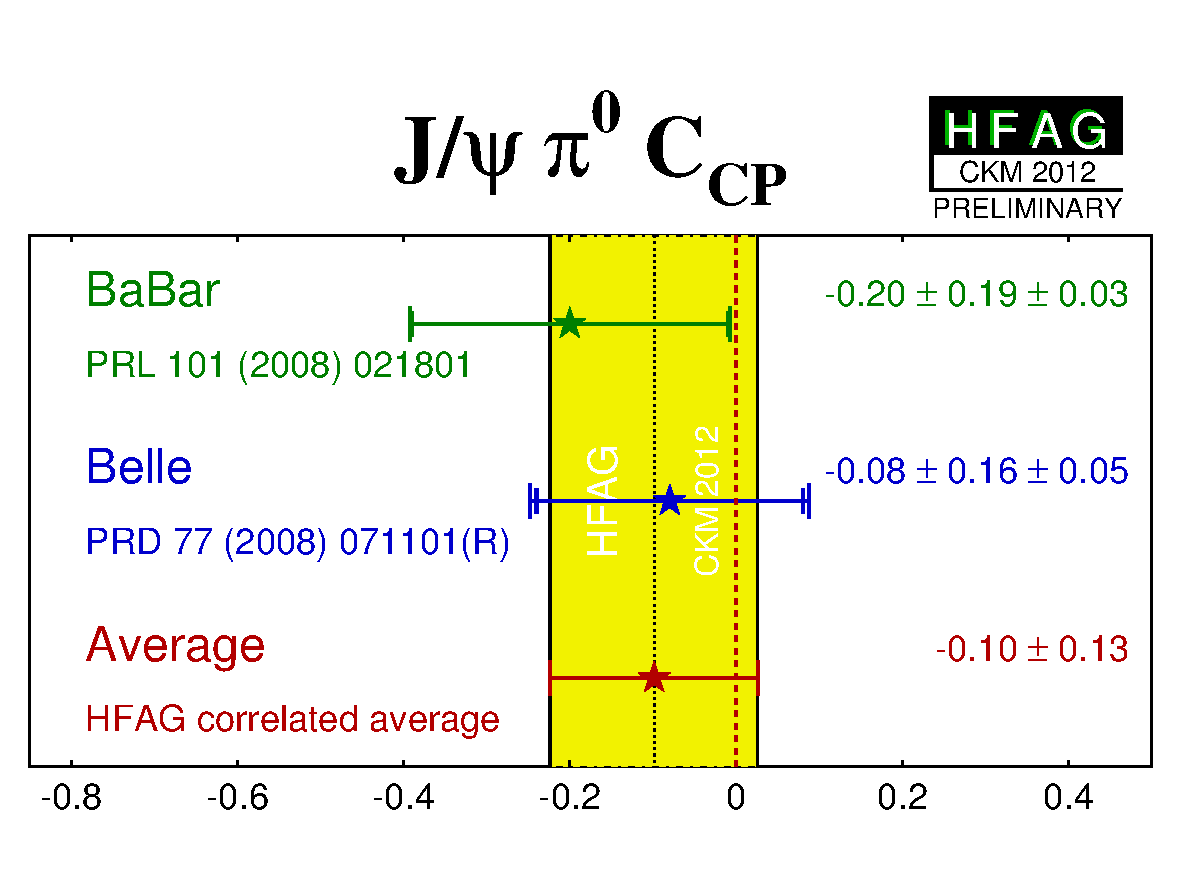
\includegraphics{figures/cp_uta/Jpsipi0C_CP}
      }
    \end{tabular}
  \end{center}
  \vspace{-0.8cm}
  \caption{
    Averages of 
    (left) $S_{b \to c\bar c d}$ and (right) $C_{b \to c\bar c d}$ 
    for the mode $\Bz \to J/ \psi \pi^0$.
  }
  \label{fig:cp_uta:ccd:psipi0}
\end{figure}

\begin{figure}[htb]
  \begin{center}
    \begin{tabular}{cc}
      \resizebox{0.46\textwidth}{!}{
        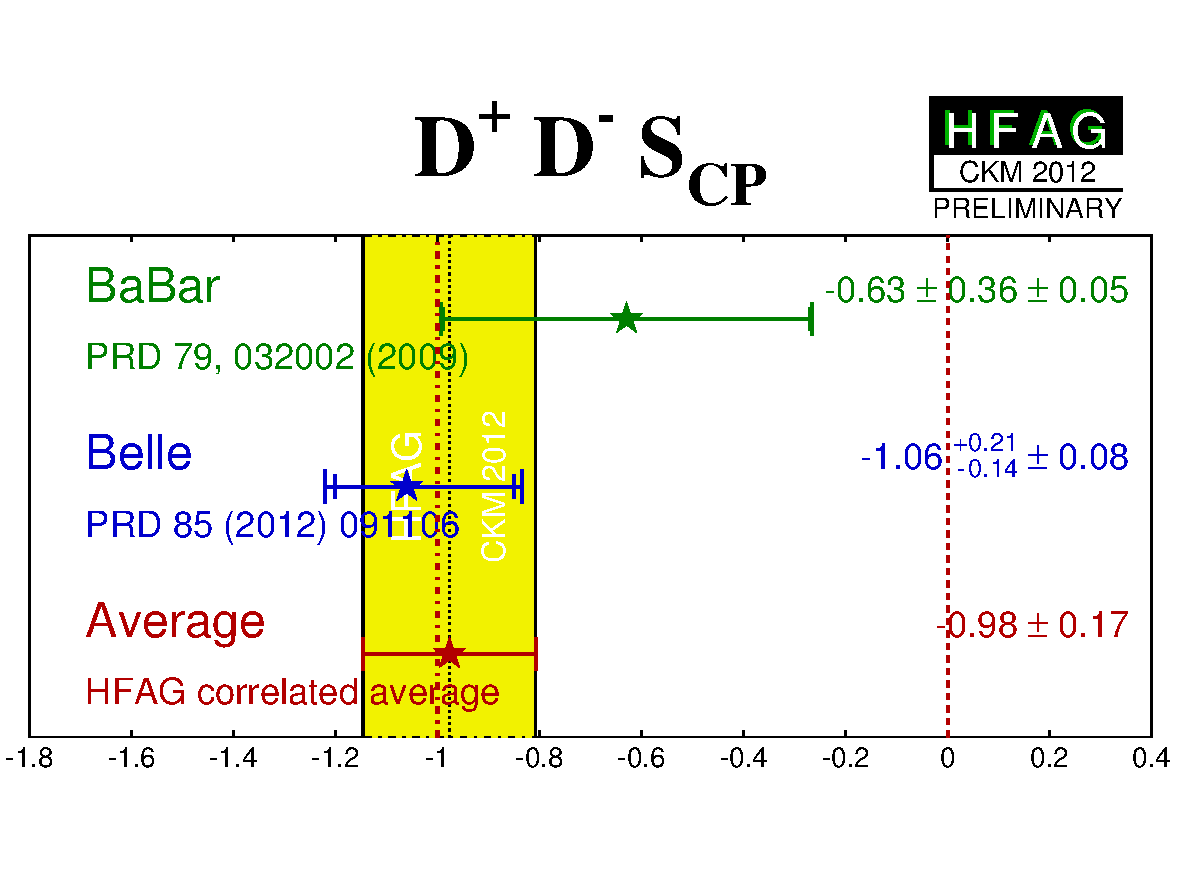
\includegraphics{figures/cp_uta/D+D-S_CP}
      }
      &
      \resizebox{0.46\textwidth}{!}{
        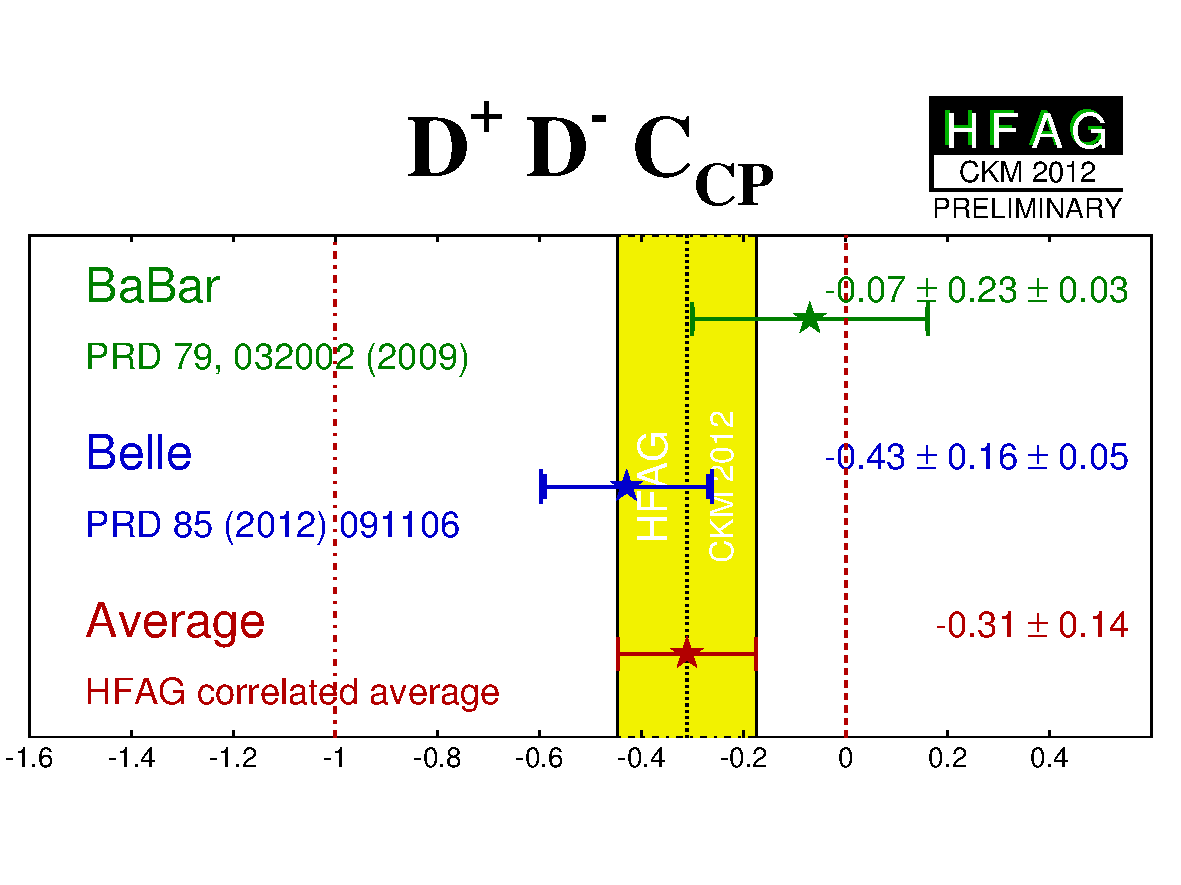
\includegraphics{figures/cp_uta/D+D-C_CP}
      }
    \end{tabular}
  \end{center}
  \vspace{-0.8cm}
  \caption{
    Averages of 
    (left) $S_{b \to c\bar c d}$ and (right) $C_{b \to c\bar c d}$ 
    for the mode $\Bz \to D^+D^-$.
  }
  \label{fig:cp_uta:ccd:dd}
\end{figure}

\begin{figure}[htb]
  \begin{center}
    \begin{tabular}{cc}
      \resizebox{0.46\textwidth}{!}{
        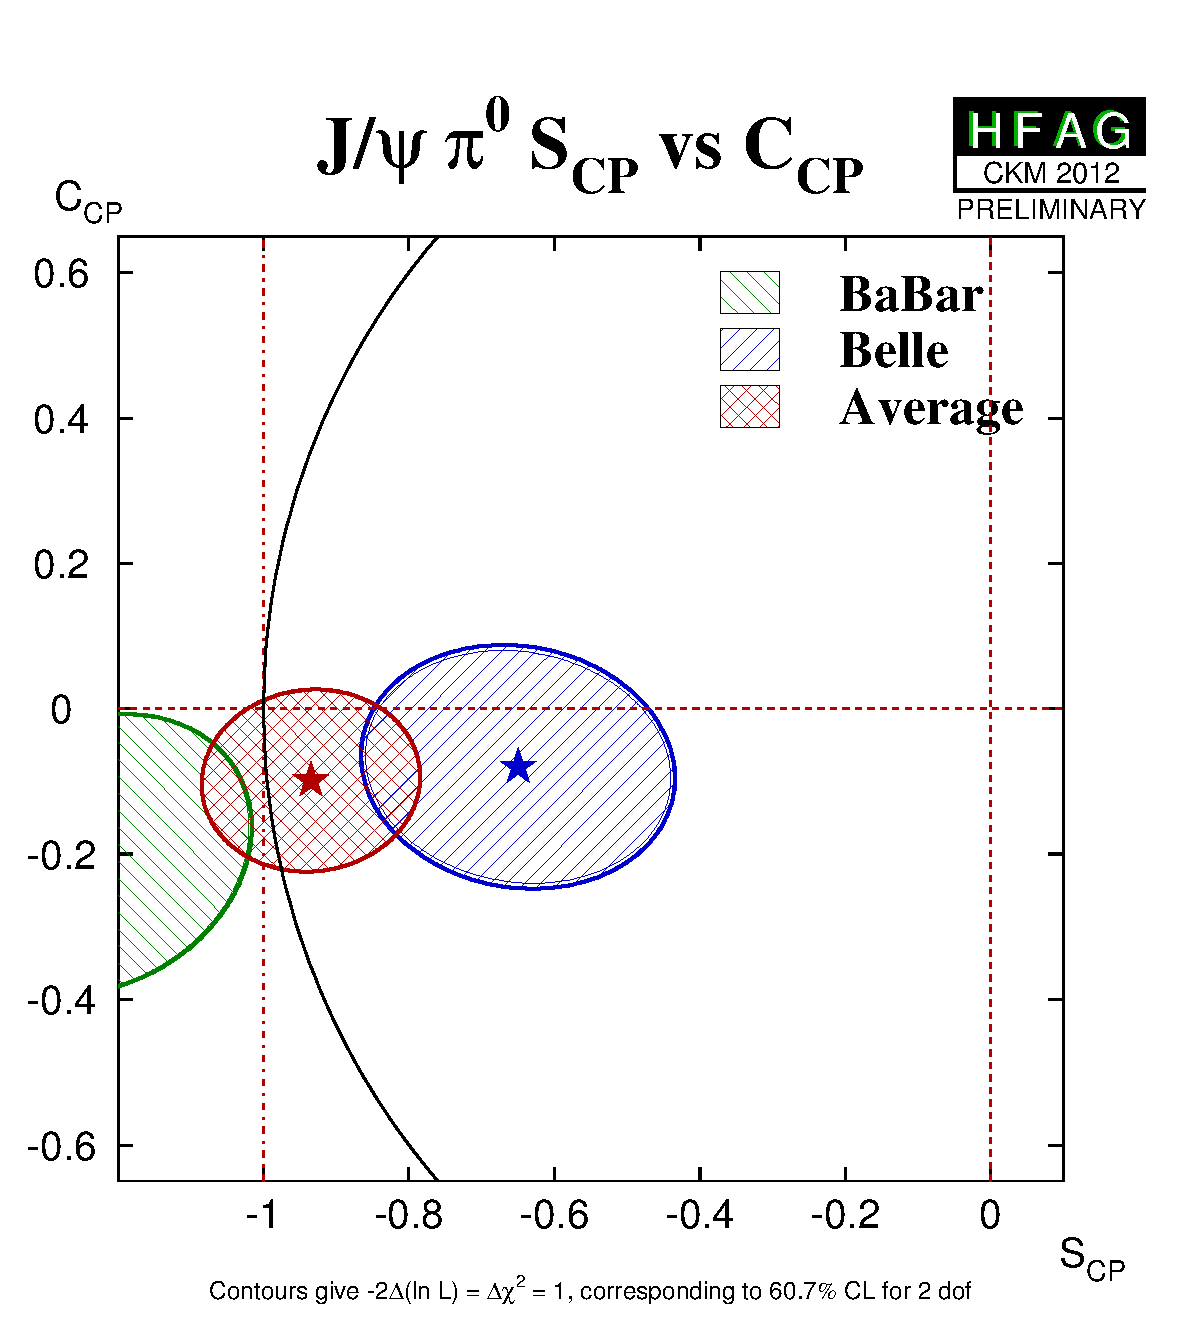
\includegraphics{figures/cp_uta/Jpsipi0S_CPvsC_CP}
      }
      &
      \resizebox{0.46\textwidth}{!}{
        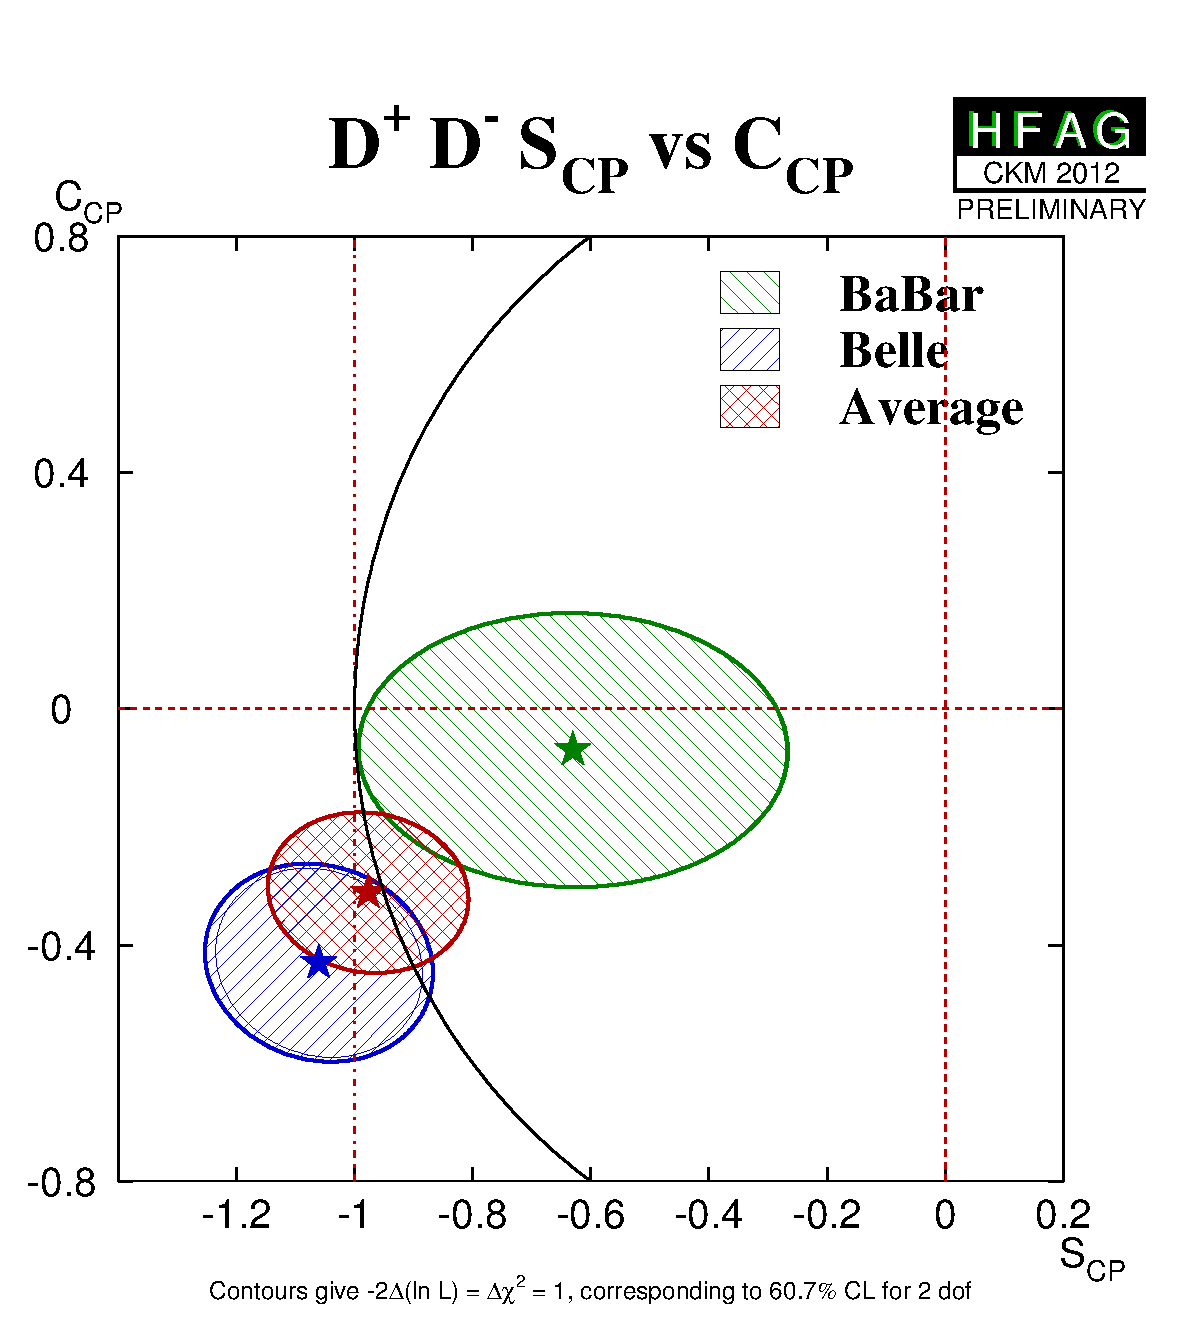
\includegraphics{figures/cp_uta/D+D-S_CPvsC_CP}
      }
    \end{tabular}
  \end{center}
  \vspace{-0.8cm}
  \caption{
    Averages of two $b \to c\bar c d$ dominated channels,
    for which correlated averages are performed,
    in the $S_{\CP}$ \vs\ $C_{\CP}$ plane.
    (Left) $\Bz \to J/ \psi \pi^0$ and (right) $\Bz \to D^+D^-$.
  }
  \label{fig:cp_uta:ccd_SvsC}
\end{figure}

\begin{figure}[htb]
  \begin{center}
    \begin{tabular}{cc}
      \resizebox{0.46\textwidth}{!}{
        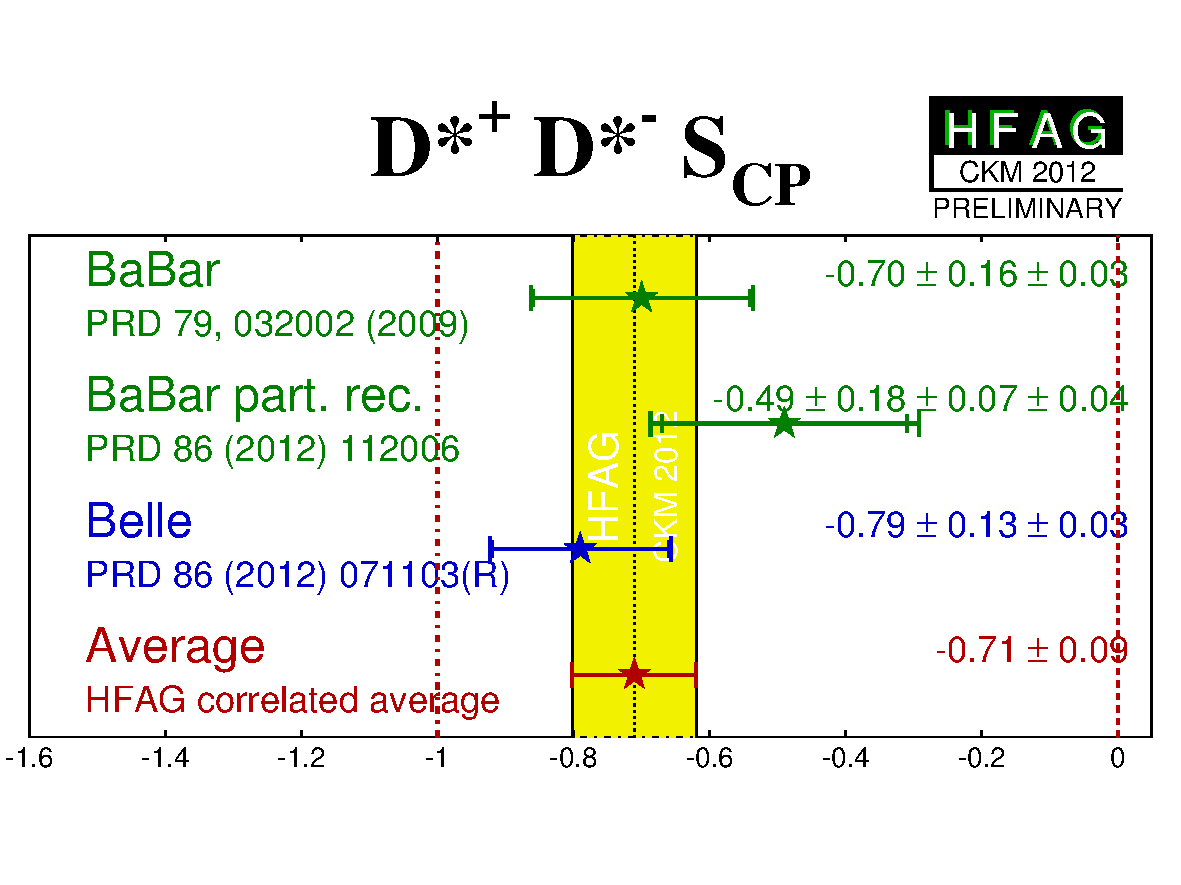
\includegraphics{figures/cp_uta/Dstar+Dstar-S_CP}
      }
      &
      \resizebox{0.46\textwidth}{!}{
        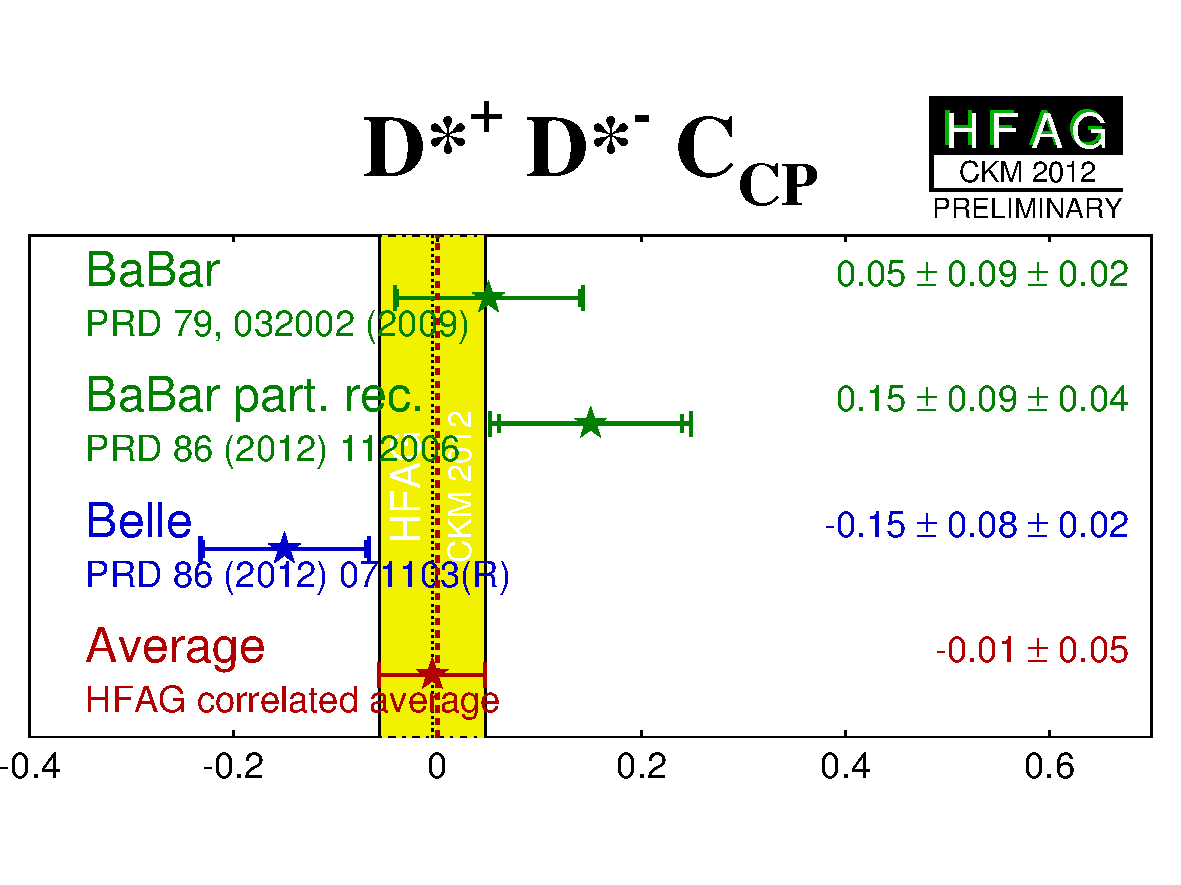
\includegraphics{figures/cp_uta/Dstar+Dstar-C_CP}
      }
    \end{tabular}
  \end{center}
  \vspace{-0.8cm}
  \caption{
    Averages of 
    (left) $S_{b \to c\bar c d}$ and (right) $C_{b \to c\bar c d}$ 
    for the mode $\Bz \to D^{*+}D^{*-}$.
  }
  \label{fig:cp_uta:ccd:dstardstar}
\end{figure}

\begin{figure}[htb]
  \begin{center}
    \begin{tabular}{cc}
      \resizebox{0.46\textwidth}{!}{
        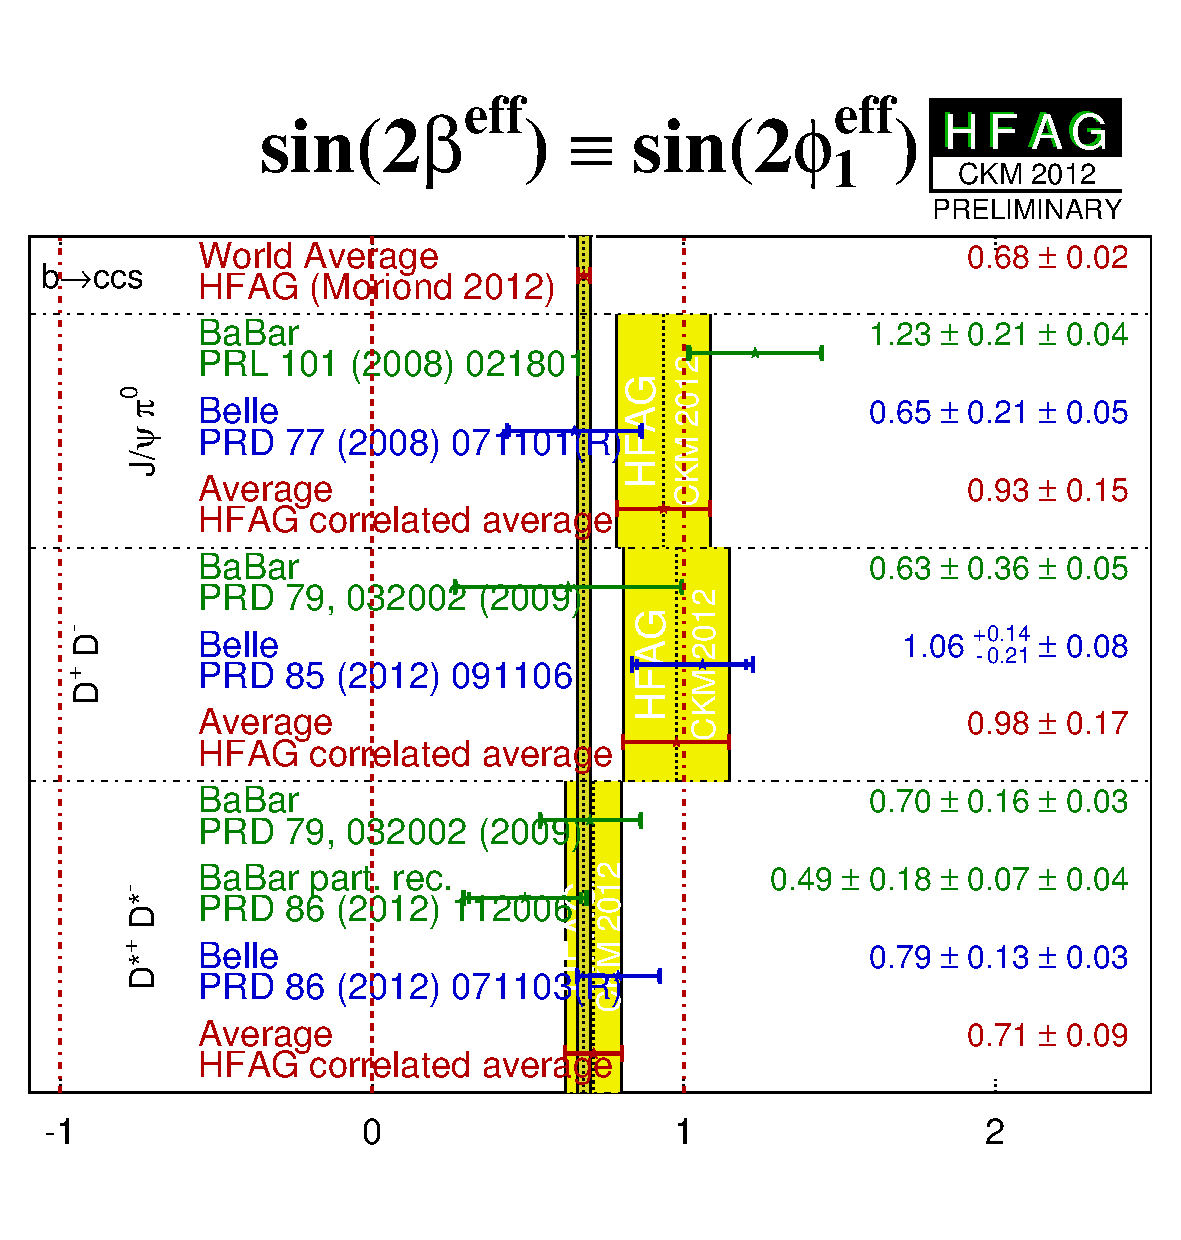
\includegraphics{figures/cp_uta/ccdS_CP}
      }
      &
      \resizebox{0.46\textwidth}{!}{
        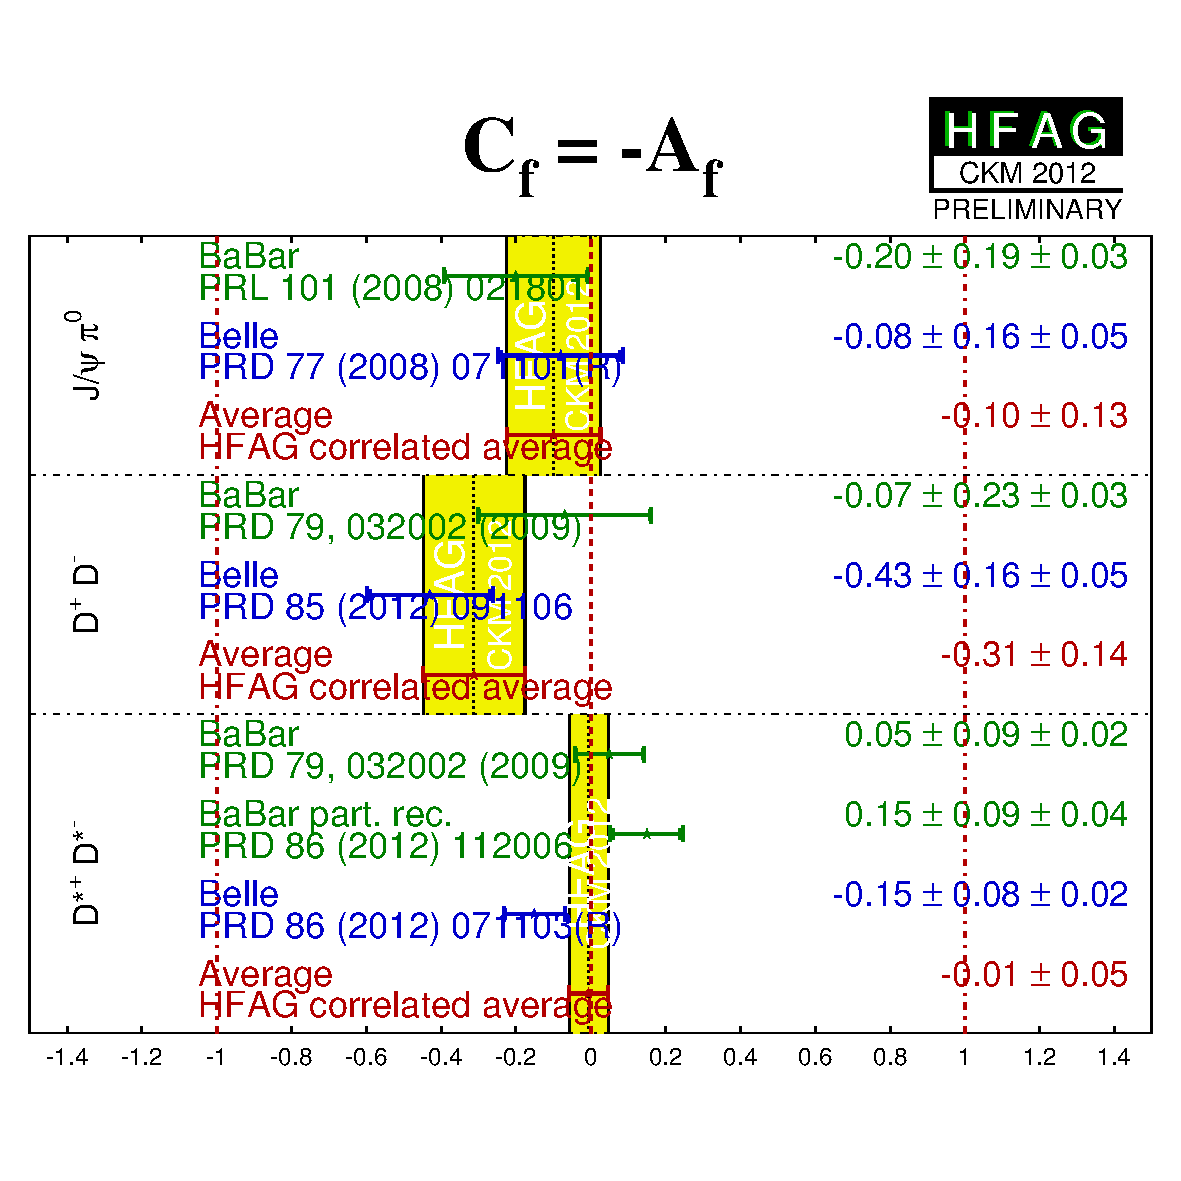
\includegraphics{figures/cp_uta/ccdC_CP}
      }
    \end{tabular}
  \end{center}
  \vspace{-0.8cm}
  \caption{
    Averages of 
    (left) $-\etacp S_{b \to c\bar c d}$ and (right) $C_{b \to c\bar c d}$.
    The $-\etacp S_{b \to q\bar q s}$ figure compares the results to 
    the world average 
    for $-\etacp S_{b \to c\bar c s}$ (see Section~\ref{sec:cp_uta:ccs:cp_eigen}).
  }
  \label{fig:cp_uta:ccd}
\end{figure}

\begin{figure}[htb]
  \begin{center}
    \resizebox{0.66\textwidth}{!}{
      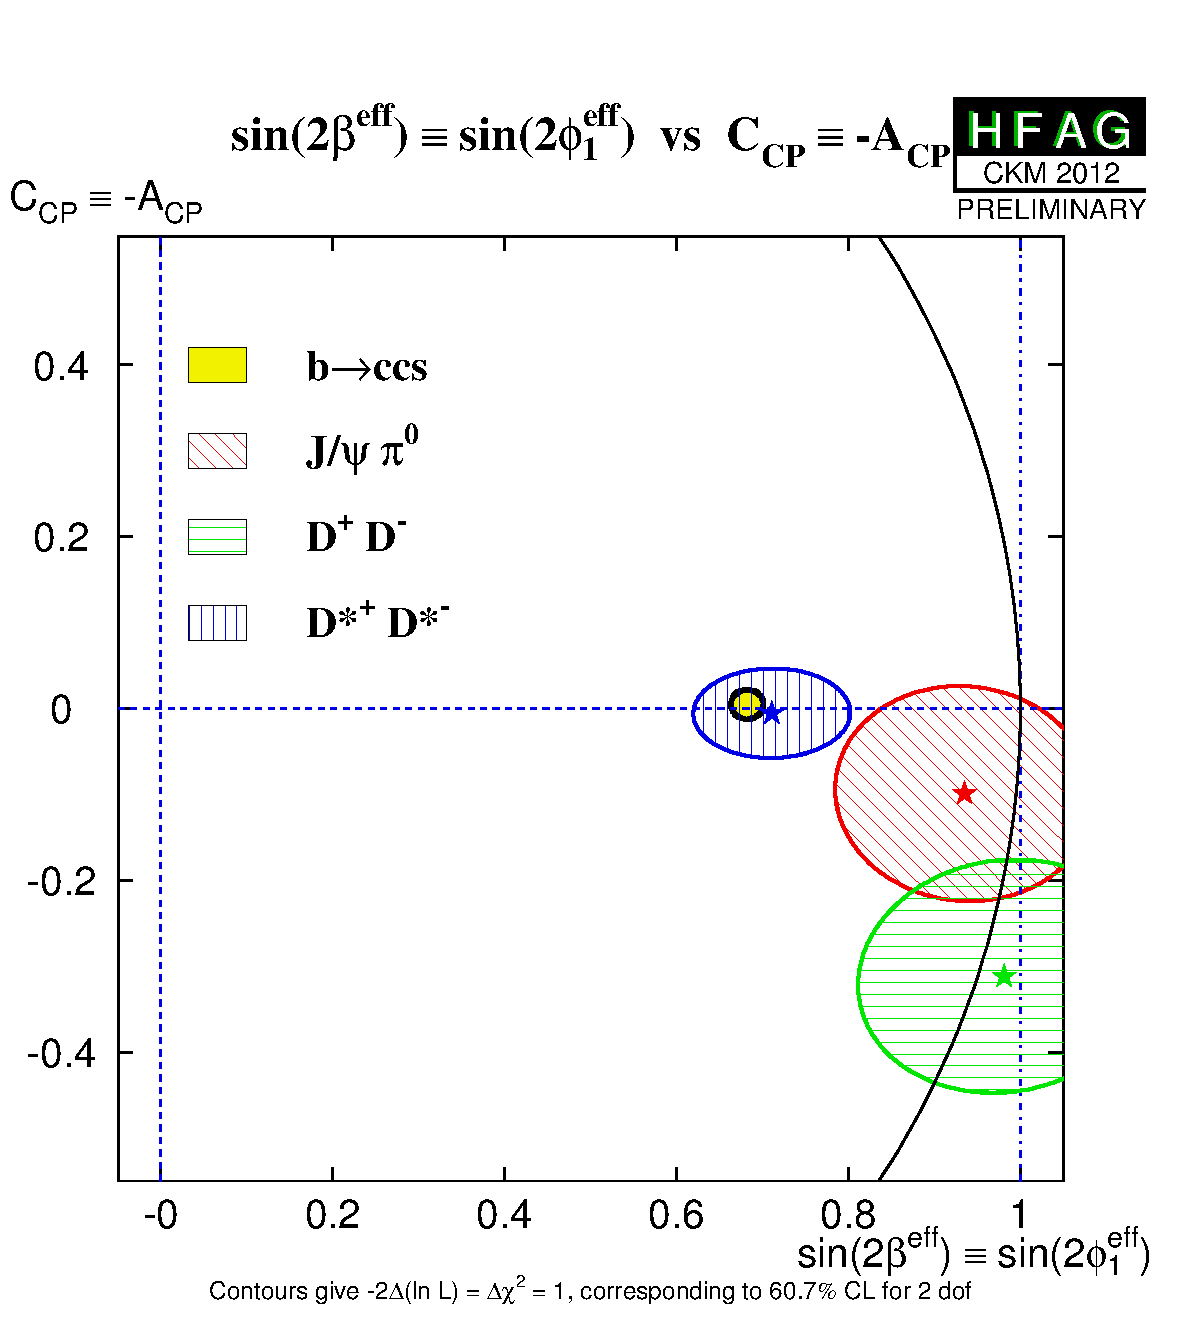
\includegraphics{figures/cp_uta/ccdS_CPvsC_CP}
    }
  \end{center}
  \vspace{-0.8cm}
  \caption{
    Compilation of constraints in the 
    $-\etacp S_{b \to c\bar c d}$ \vs\ $C_{b \to c\bar c d}$ plane.
  }
  \label{fig:cp_uta:ccd_SvsC-all}
\end{figure}

%% straightforward interpretation

%%%%%%%%
%%%
%%% qqd
%%%
%%%%%%%%
\clearpage
\mysubsection{Time-dependent $\CP$ asymmetries in $b \to q\bar{q}d$ transitions
}
\label{sec:cp_uta:qqd}

Decays such as $\Bz\to\KS\KS$ are pure $b \to q\bar{q}d$ penguin transitions.
As shown in Eq.~\ref{eq:cp_uta:b_to_d},
this diagram has different contributing weak phases,
and therefore the observables are sensitive to the difference 
(which can be chosen to be either $\beta$ or $\gamma$).
Note that if the contribution with the top quark in the loop dominates,
the weak phase from the decay amplitudes should cancel that from mixing,
so that no $\CP$ violation (neither mixing-induced nor in decay) occurs.
Non-zero contributions from loops with intermediate up and charm quarks
can result in both types of effect 
(as usual, a strong phase difference is required for $\CP$ violation in decay
to occur).

Both \babar~\cite{Aubert:2006gm} and \belle~\cite{Nakahama:2007dg}
have performed time-dependent analyses of $\Bz\to\KS\KS$.
The results are shown in Table~\ref{tab:cp_uta:qqd}
and Fig.~\ref{fig:cp_uta:qqd:ksks}.

\begin{table}[htb]
	\begin{center}
		\caption{
			Results for $\Bz \to \KS\KS$.
		}
		\vspace{0.2cm}
		\setlength{\tabcolsep}{0.0pc}
		\begin{tabular*}{\textwidth}{@{\extracolsep{\fill}}lrcccc} \hline
	\mc{2}{l}{Experiment} & $N(B\bar{B})$ & $S_{CP}$ & $C_{CP}$ & Correlation \\
	\hline
	\babar & \cite{Aubert:2006gm} & 350M & $-1.28 \,^{+0.80}_{-0.73} \,^{+0.11}_{-0.16}$ & $-0.40 \pm 0.41 \pm 0.06$ & $-0.32$ \\
	\belle & \cite{Nakahama:2007dg} & 657M & $-0.38 \,^{+0.69}_{-0.77} \pm 0.09$ & $0.38 \pm 0.38 \pm 0.05$ & $0.48$ \\
	\hline
	\mc{3}{l}{\bf Average} & $-1.08 \pm 0.49$ & $-0.06 \pm 0.26$ & $0.14$ \\
	\mc{3}{l}{\small Confidence level} & \mc{2}{c}{\small $0.29~(1.1\sigma)$} & \\
		\hline
		\end{tabular*}
		\label{tab:cp_uta:qqd}
	\end{center}
\end{table}




\begin{figure}[htb]
  \begin{center}
    \begin{tabular}{cc}
      \resizebox{0.46\textwidth}{!}{
        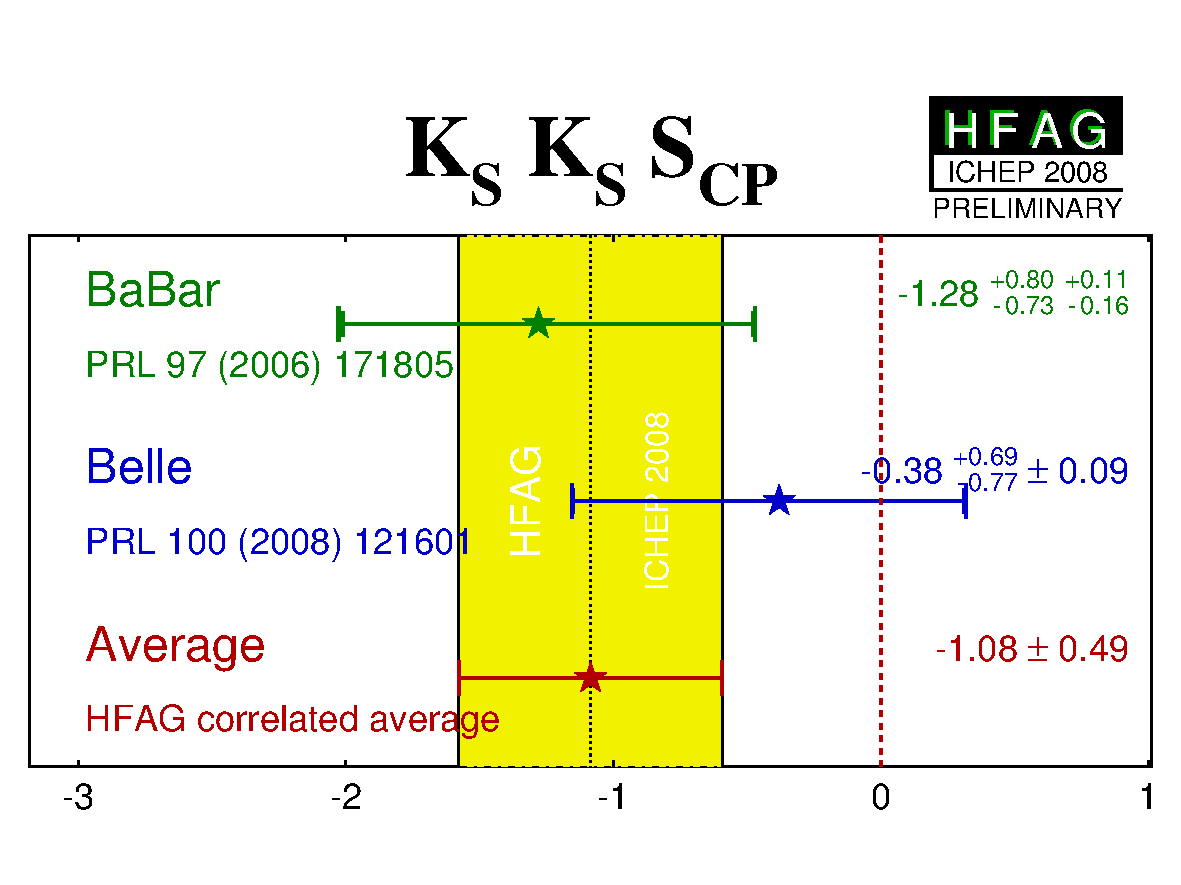
\includegraphics{figures/cp_uta/KSKSS_CP}
      }
      &
      \resizebox{0.46\textwidth}{!}{
        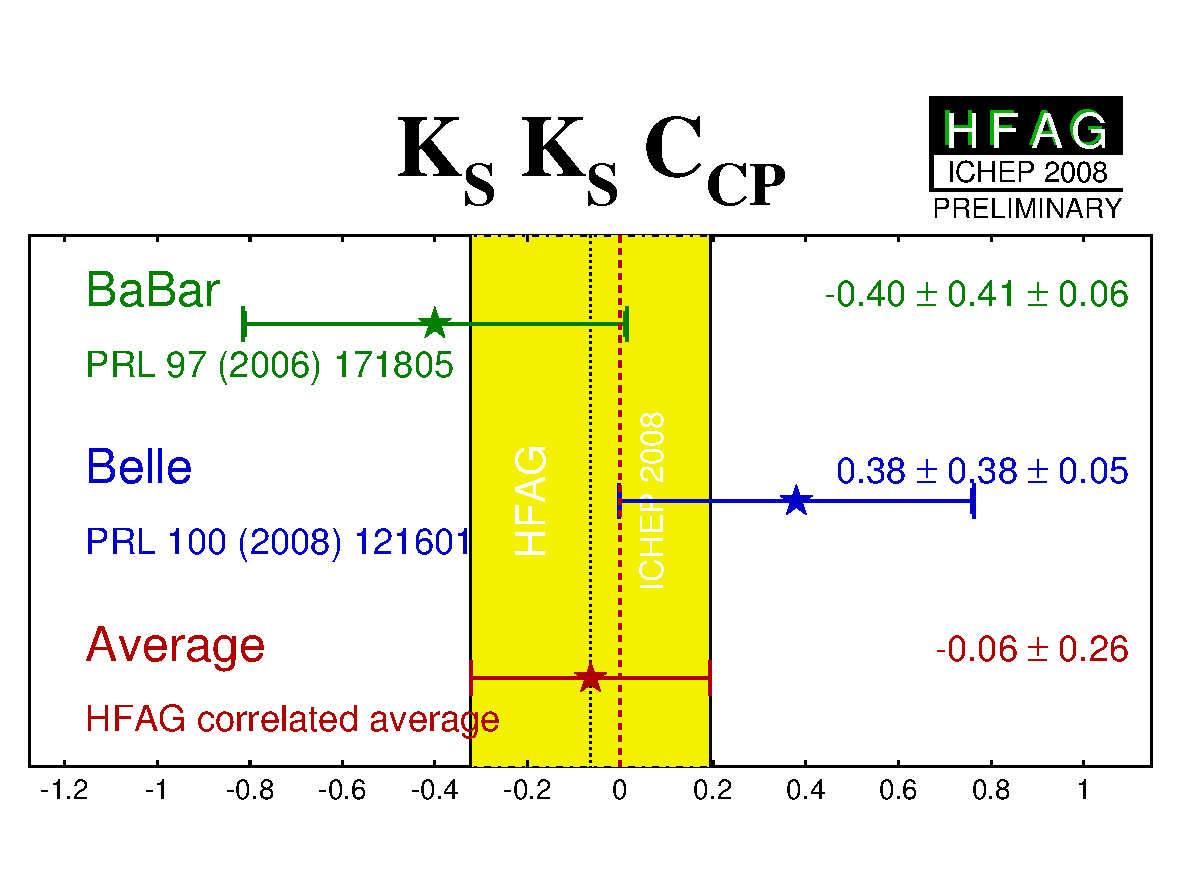
\includegraphics{figures/cp_uta/KSKSC_CP}
      }
    \end{tabular}
  \end{center}
  \vspace{-0.8cm}
  \caption{
    Averages of 
    (left) $S_{b \to q\bar q d}$ and (right) $C_{b \to q\bar q d}$ 
    for the mode $\Bz \to \KS\KS$.
  }
  \label{fig:cp_uta:qqd:ksks}
\end{figure}

%%%%%%%%
%%%
%%% b -> sg
%%%
%%%%%%%%
\clearpage
\mysubsection{Time-dependent asymmetries in $b \to s\gamma$ transitions
}
\label{sec:cp_uta:bsg}

The radiative decays $b \to s\gamma$ produce photons 
which are highly polarised in the Standard Model.
The decays $\Bz \to F \gamma$ and $\Bzb \to F \gamma$ 
produce photons with opposite helicities, 
and since the polarisation is, in principle, observable,
these final states cannot interfere.
The finite mass of the $s$ quark introduces small corrections
to the limit of maximum polarisation,
but any large mixing induced $\CP$ violation would be a signal for new physics.
Since a single weak phase dominates the $b \to s \gamma$ transition in the 
Standard Model, the cosine term is also expected to be small.

Atwood {\it et al.}~\cite{Atwood:2004jj} have shown that 
an inclusive analysis with respect to $\KS\pi^0\gamma$ can be performed,
since the properties of the decay amplitudes 
are independent of the angular momentum of the $\KS\pi^0$ system. 
However, if non-dipole operators contribute significantly to the amplitudes, 
then the Standard Model mixing-induced $\CP$ violation could be larger 
than the na\"\i ve expectation 
$S \simeq -2 (m_s/m_b) \sin \left(2\beta\right)$~\cite{Grinstein:2004uu,Grinstein:2005nu}.
In this case, 
the $\CP$ parameters may vary over the $\KS\pi^0\gamma$ Dalitz plot, 
for example as a function of the $\KS\pi^0$ invariant mass.
Explicit calculations indicate such corrections are small
for exclusive final states~\cite{Matsumori:2005ax,Ball:2006cva}.

With the above in mind, 
we quote two averages: one for $K^*(892)$ candidates only, 
and the other one for the inclusive $\KS\pi^0\gamma$ decay (including the $K^*(892)$).
If the Standard Model dipole operator is dominant, 
both should give the same quantities 
(the latter naturally with smaller statistical error). 
If not, care needs to be taken in interpretation of the inclusive parameters, 
while the results on the $K^*(892)$ resonance remain relatively clean.
Results from \babar\ and \belle\ are
used for both averages; both experiments use the invariant mass range 
$0.60 \ {\rm GeV}/c^2 < M_{\KS\pi^0} < 1.80 \ {\rm GeV}/c^2$
in the inclusive analysis.

In addition to the $\KS\pi^0\gamma$ decay, both \babar\ and \belle\ have presented results using $\KS\eta\gamma$ and $\KS\rho\gamma$, and \belle\ have in addition presented results using $\KS\phi\gamma$.
For the $\KS\rho\gamma$ case, due to the non-negligible width of the $\rho^0$ meson, decays selected as $\Bz \to \KS\rho^0\gamma$ can include a significant contribution from $K^{*\pm}\pi^\mp\gamma$ decays, which are flavour-specific and do not have the same oscillation phenomenology. 
Both \babar\ and \belle\ measure $S_{\rm eff}$ for all \B decay candidates with the $\rho^0$ selection being $0.6 < m(\pip\pim) < 0.9 \ {\rm GeV}/c^2$, obtaining $0.14 \pm 0.25 \,^{+0.04}_{-0.03}$ (\babar) and $0.09 \pm 0.27 \,^{+0.04}_{-0.07}$ (\belle). These values are then corrected for a ``dilution factor'', that is evaluated with different methods in the two experiments: \babar~\cite{Akar:2013ima} obtain $0.549 \,^{+0.096}_{-0.094}$ while \belle~\cite{Li:2008qma} obtain $0.83 \,^{+0.19}_{-0.03}$. Until the discrepancy between these values is understood, the average of the results should be treated with caution.


\begin{table}[htb]
	\begin{center}
		\caption{
      Averages for $b \to s \gamma$ modes.
		}
		\vspace{0.2cm}
		\setlength{\tabcolsep}{0.0pc}
		\begin{tabular*}{\textwidth}{@{\extracolsep{\fill}}lrcccc} \hline
	\mc{2}{l}{Experiment} & $N(B\bar{B})$ & $S_{CP} (b \to s \gamma)$ & $C_{CP} (b \to s \gamma)$ & Correlation \\
        \hline
        \mc{6}{c}{$\Kstar(892)\gamma$} \\
	\babar & \cite{Aubert:2008gy} & 467M & $-0.03 \pm 0.29 \pm 0.03$ & $-0.14 \pm 0.16 \pm 0.03$ & $0.05$ \\
	\belle & \cite{Ushiroda:2006fi} & 535M & $-0.32 \,^{+0.36}_{-0.33} \pm 0.05$ & $0.20 \pm 0.24 \pm 0.05$ & $0.08$ \\
%	\hline
	\mc{3}{l}{\bf Average} & $-0.16 \pm 0.22$ & $-0.04 \pm 0.14$ & $0.06$ \\
	\mc{3}{l}{\small Confidence level} & \mc{2}{c}{\small $0.40~(0.9\sigma)$} & \\
		\hline
% 		\end{tabular*}
% 		\label{tab:cp_uta:yyy}
% 	\end{center}
% \end{table}


% \begin{table}
% 	\begin{center}
% 		\caption{
% 			Averages for $K_{S} \\pi^{0} \\gammama$.
% 		}
% 		\vspace{0.2cm}
% 		\setlength{\tabcolsep}{0.0pc}
% 		\begin{tabular*}{\textwidth}{@{\extracolsep{\fill}}lrcccc} \hline
% 		\mc{2}{l}{Experiment} & $N(B\bar{B})$ & $S_{CP}$ & $C_{CP}$ & Correlation \\
% 		\hline
        \mc{6}{c}{$\KS \pi^0 \gamma$ (including $\Kstar(892)\gamma$)} \\
	\babar & \cite{Aubert:2008gy} & 467M & $-0.17 \pm 0.26 \pm 0.03$ & $-0.19 \pm 0.14 \pm 0.03$ & $0.04$ \\
	\belle & \cite{Ushiroda:2006fi} & 535M & $-0.10 \pm 0.31 \pm 0.07$ & $0.20 \pm 0.20 \pm 0.06$ & $0.08$ \\
%	\hline
	\mc{3}{l}{\bf Average} & $-0.15 \pm 0.20$ & $-0.07 \pm 0.12$ & $0.05$ \\
        \mc{3}{l}{\small Confidence level} & \mc{2}{c}{\small $0.30~(1.0\sigma)$} & \\

		\hline
%% 		\end{tabular*}
%% 		\label{tab:cp_uta:bsg}
%% 	\end{center}
%% \end{table}

%% \begin{table}[!htb]
%% 	\begin{center}
%% 		\caption{
%% 			Averages for $K_{S} eta \\gammama$.
%% 		}
%% 		\vspace{0.2cm}
%% 		\setlength{\tabcolsep}{0.0pc}
%% 		\begin{tabular*}{\textwidth}{@{\extracolsep{\fill}}lrcccc} \hline
%% 	\mc{2}{l}{Experiment} & $N(B\bar{B})$ & $S_{CP}$ & $C_{CP}$ & Correlation \\
%% 	\hline
        \mc{6}{c}{$\KS \eta \gamma$} \\
	\babar & \cite{Aubert:2008js} & 465M & $-0.18 \,^{+0.49}_{-0.46} \pm 0.12$ & $-0.32 \,^{+0.40}_{-0.39} \pm 0.07$ & $-0.17$ \\
	\belle & \cite{} & 772M & $-1.32 \pm 0.77 \pm 0.36$ & $0.48 \pm 0.41 \pm 0.07$ & $-0.14$ \\
	\hline
	\mc{3}{l}{\bf Average} & $-0.49 \pm 0.42$ & $0.06 \pm 0.29$ & $-0.15$ \\
	\mc{3}{l}{\small Confidence level} & \mc{2}{c}{\small $0.24~(1.2\sigma)$} & \\
%% 		\hline
%% 		\end{tabular*}
%% 		\label{tab:cp_uta:yyy}
%% 	\end{center}
%% \end{table}


%% \begin{table}[!htb]
%% 	\begin{center}
%% 		\caption{
%% 			Averages for $K_{S} \\rho^{0} \\gammama$.
%% 		}
%% 		\vspace{0.2cm}
%% 		\setlength{\tabcolsep}{0.0pc}
%% 		\begin{tabular*}{\textwidth}{@{\extracolsep{\fill}}lrcccc} \hline
%% 	\mc{2}{l}{Experiment} & $N(B\bar{B})$ & $S_{CP}$ & $C_{CP}$ & Correlation \\
%% 	\hline
        \mc{6}{c}{$\KS \rho^0 \gamma$} \\
	\babar & \cite{Akar:2014hda} & 471M & $0.25 \pm 0.46 \,^{+0.08}_{-0.06}$ & $-0.39 \pm 0.20 \pm 0.05$ & $-0.09$ \\
	\belle & \cite{Li:2008qma} & 657M & $0.11 \pm 0.33 \,^{+0.05}_{-0.09}$ & $-0.05 \pm 0.18 \pm 0.06$ & $\phantom{-}0.04$ \\
	\hline
	\mc{3}{l}{\bf Average} & $0.14 \pm 0.27$ & $-0.20 \pm 0.14$ & $-0.01$ \\
	\mc{3}{l}{\small Confidence level} & \mc{2}{c}{\small $0.47~(0.7\sigma)$} & \\
%% 		\hline
%% 		\end{tabular*}
%% 		\label{tab:cp_uta:bsg}
%% 	\end{center}
%% \end{table}

%% \begin{table}[!htb]
%% 	\begin{center}
%% 		\caption{
%% 			Averages for $K_{S} \phi \\gammama$.
%% 		}
%% 		\vspace{0.2cm}
%% 		\setlength{\tabcolsep}{0.0pc}
%% 		\begin{tabular*}{\textwidth}{@{\extracolsep{\fill}}lrcccc} \hline
%% 	\mc{2}{l}{Experiment} & $N(B\bar{B})$ & $S_{CP}$ & $C_{CP}$ & Correlation \\
	%% \hline
        \mc{6}{c}{$\KS \phi \gamma$} \\
	\belle & \cite{Sahoo:2011zd} & 772M & $0.74 \,^{+0.72}_{-1.05} \,^{+0.10}_{-0.24}$ & $-0.35 \pm 0.58 \,^{+0.10}_{-0.23}$ & \textendash{} \\
	\hline
	%% \mc{3}{l}{\bf Average} & $0.74 \pm 0.90$ & $-0.35 \pm 0.60$ & $0.00$ \\
	%% \mc{3}{l}{\small Confidence level} & \mc{2}{c}{\small $0.xx~(y.y\sigma)$} & \\
	%% 	\hline
		\end{tabular*}
		\label{tab:cp_uta:bsg}
	\end{center}
\end{table}




The results are shown in Table~\ref{tab:cp_uta:bsg},
and in Figs.~\ref{fig:cp_uta:bsg} and~~\ref{fig:cp_uta:bsg_SvsC}.
No significant $\CP$ violation results are seen;
the results are consistent with the Standard Model
and with other measurements in the $b \to s\gamma$ system (see Sec.~\ref{sec:rare}).

\begin{figure}[htb]
  \begin{center}
    \begin{tabular}{cc}
      \resizebox{0.46\textwidth}{!}{
        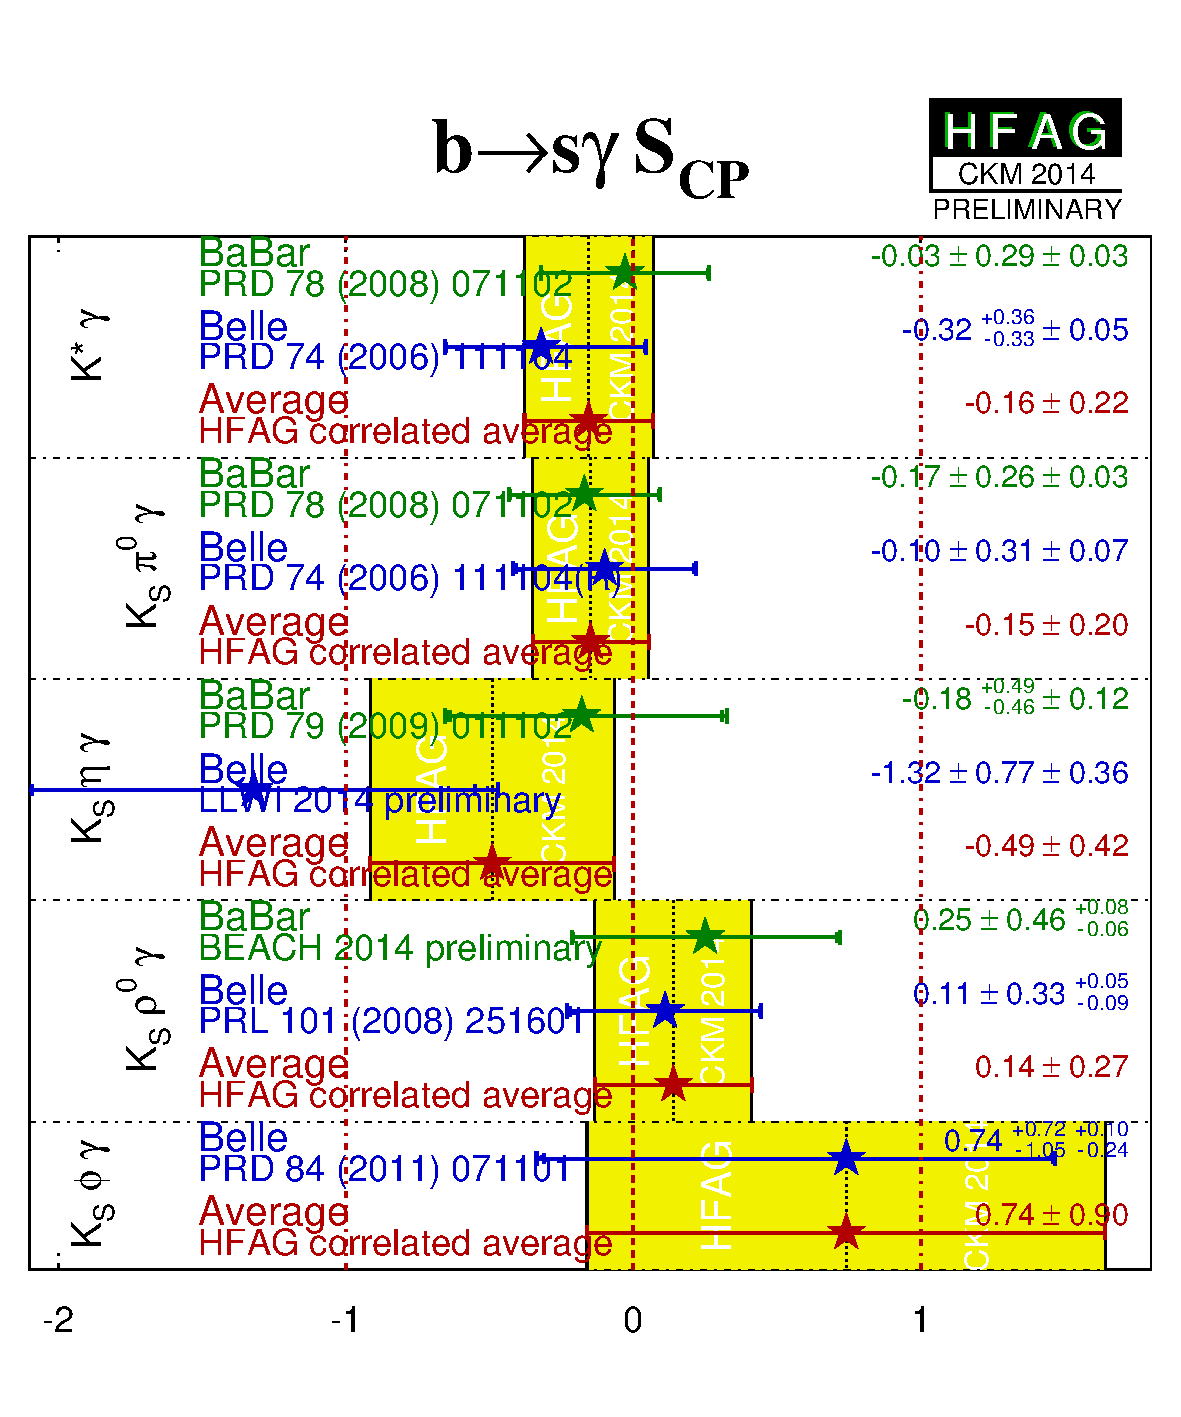
\includegraphics{figures/cp_uta/bsgS_CP}
      }
      &
      \resizebox{0.46\textwidth}{!}{
        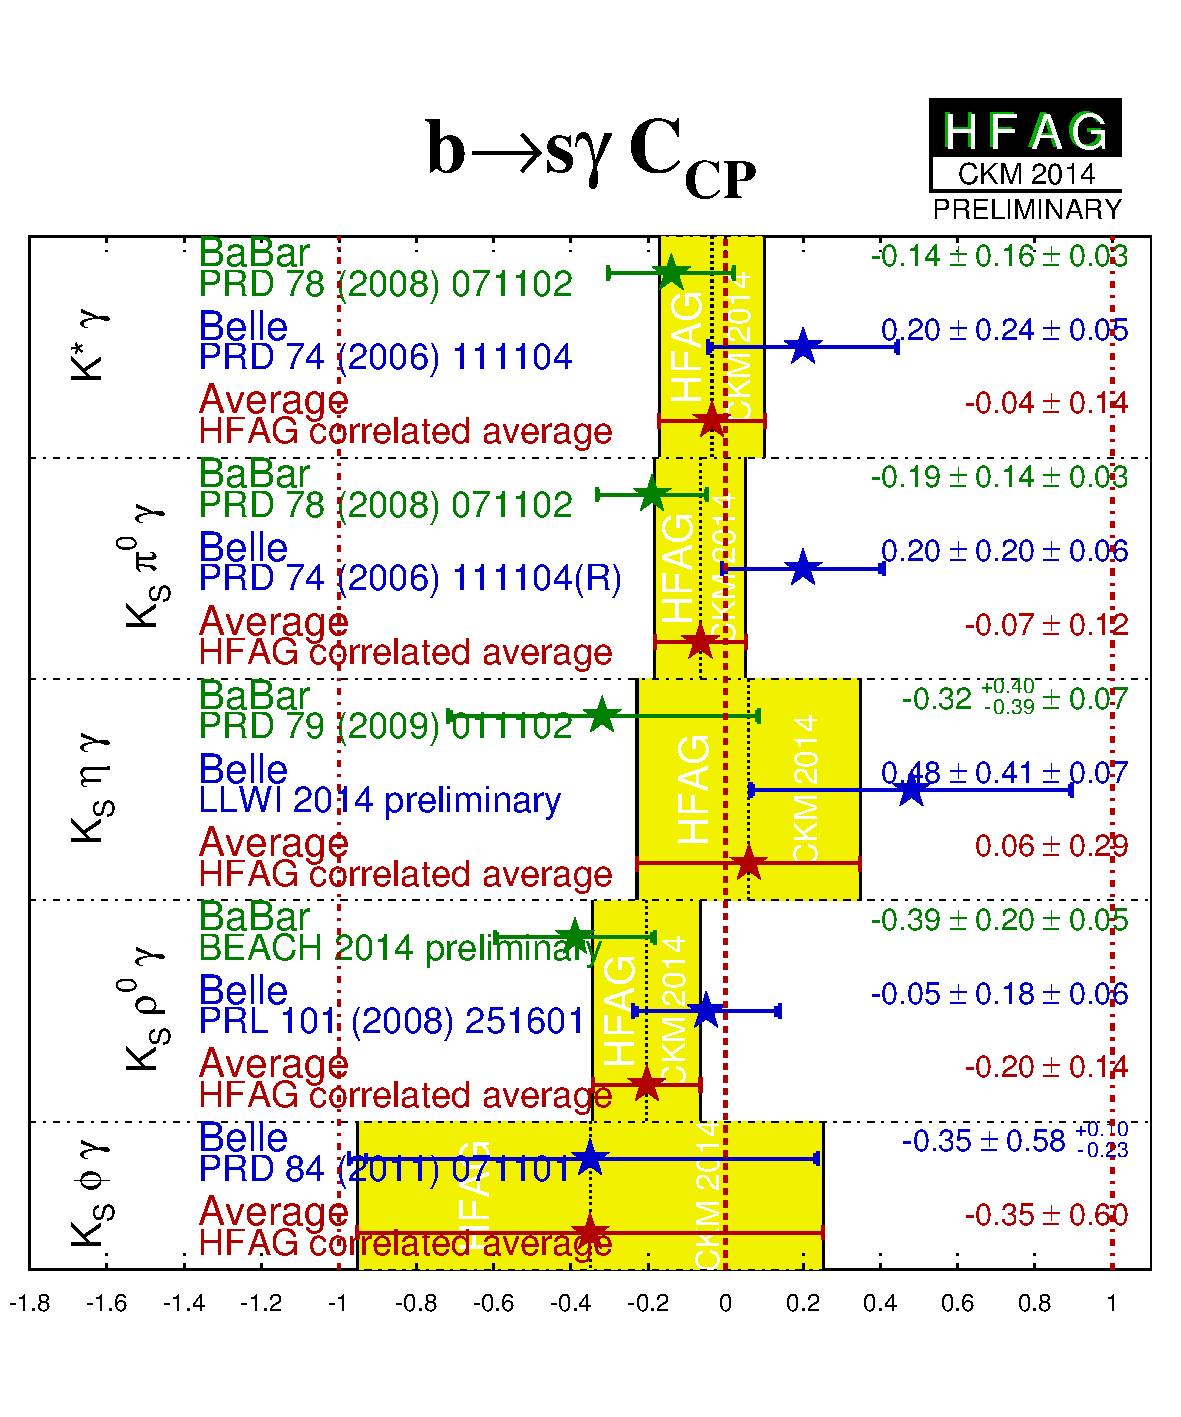
\includegraphics{figures/cp_uta/bsgC_CP}
      }
    \end{tabular}
  \end{center}
  \vspace{-0.8cm}
  \caption{
    Averages of (left) $S_{b \to s \gamma}$ and (right) $C_{b \to s \gamma}$.
    Recall that the data for $K^*\gamma$ is a subset of that for $\KS\pi^0\gamma$.
  }
  \label{fig:cp_uta:bsg}
\end{figure}

\begin{figure}[htb]
  \begin{center}
    \resizebox{0.33\textwidth}{!}{
      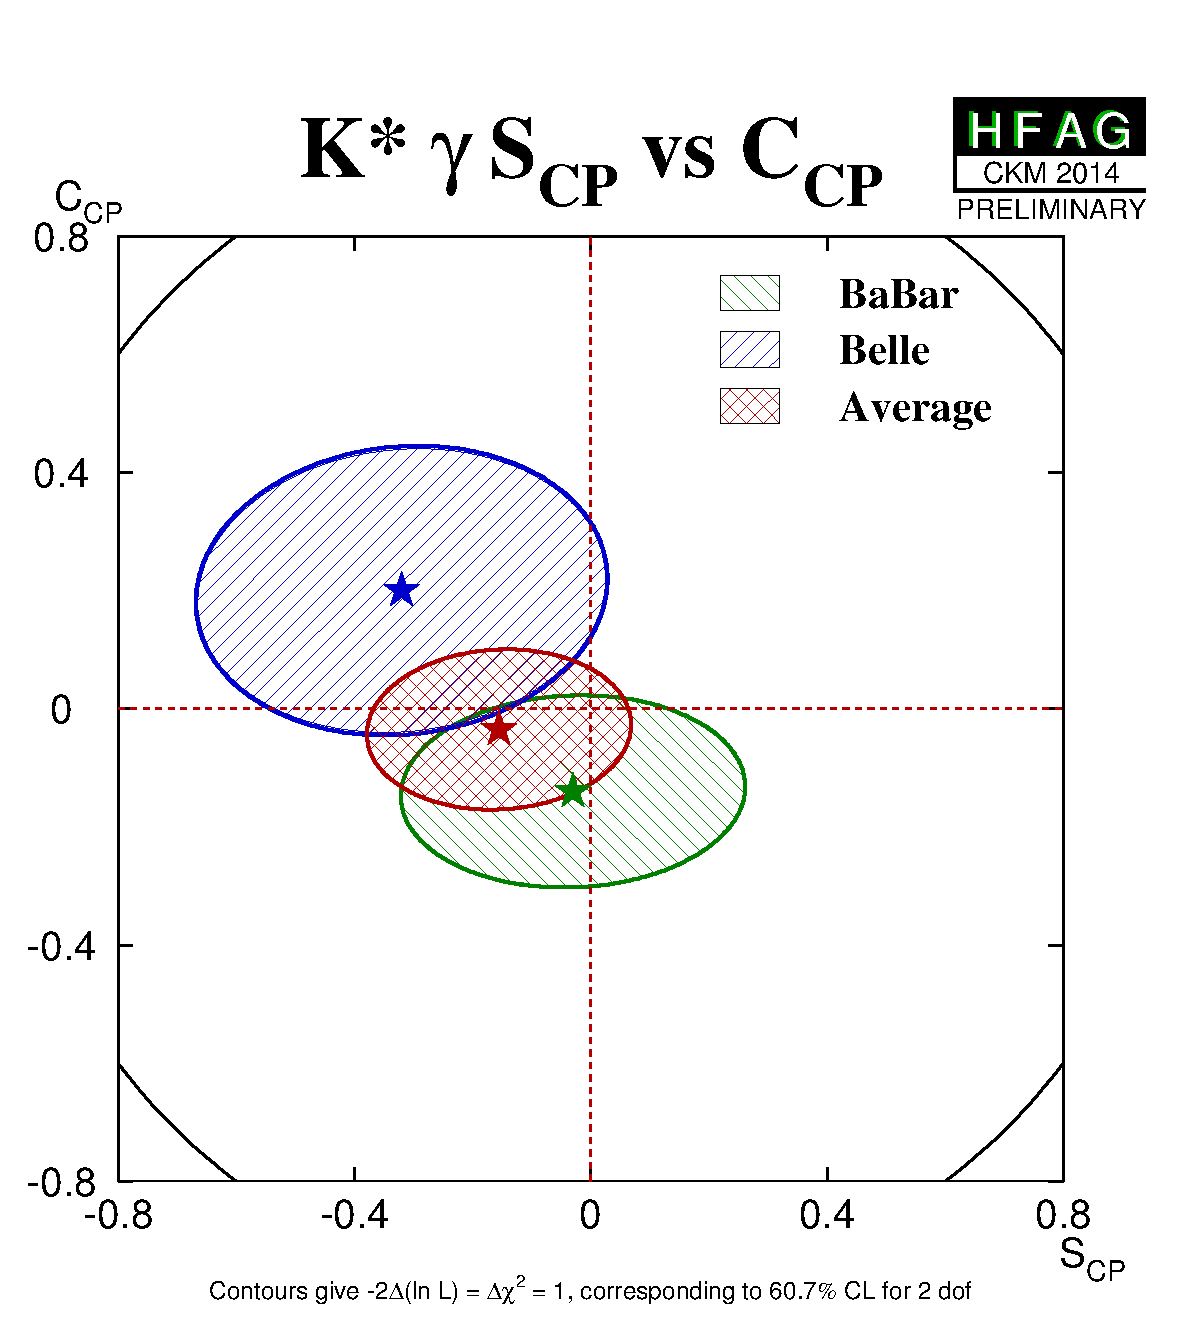
\includegraphics{figures/cp_uta/KstargammaS_CPvsC_CP}
    }
    \hspace{0.08\textwidth}
    \resizebox{0.33\textwidth}{!}{
      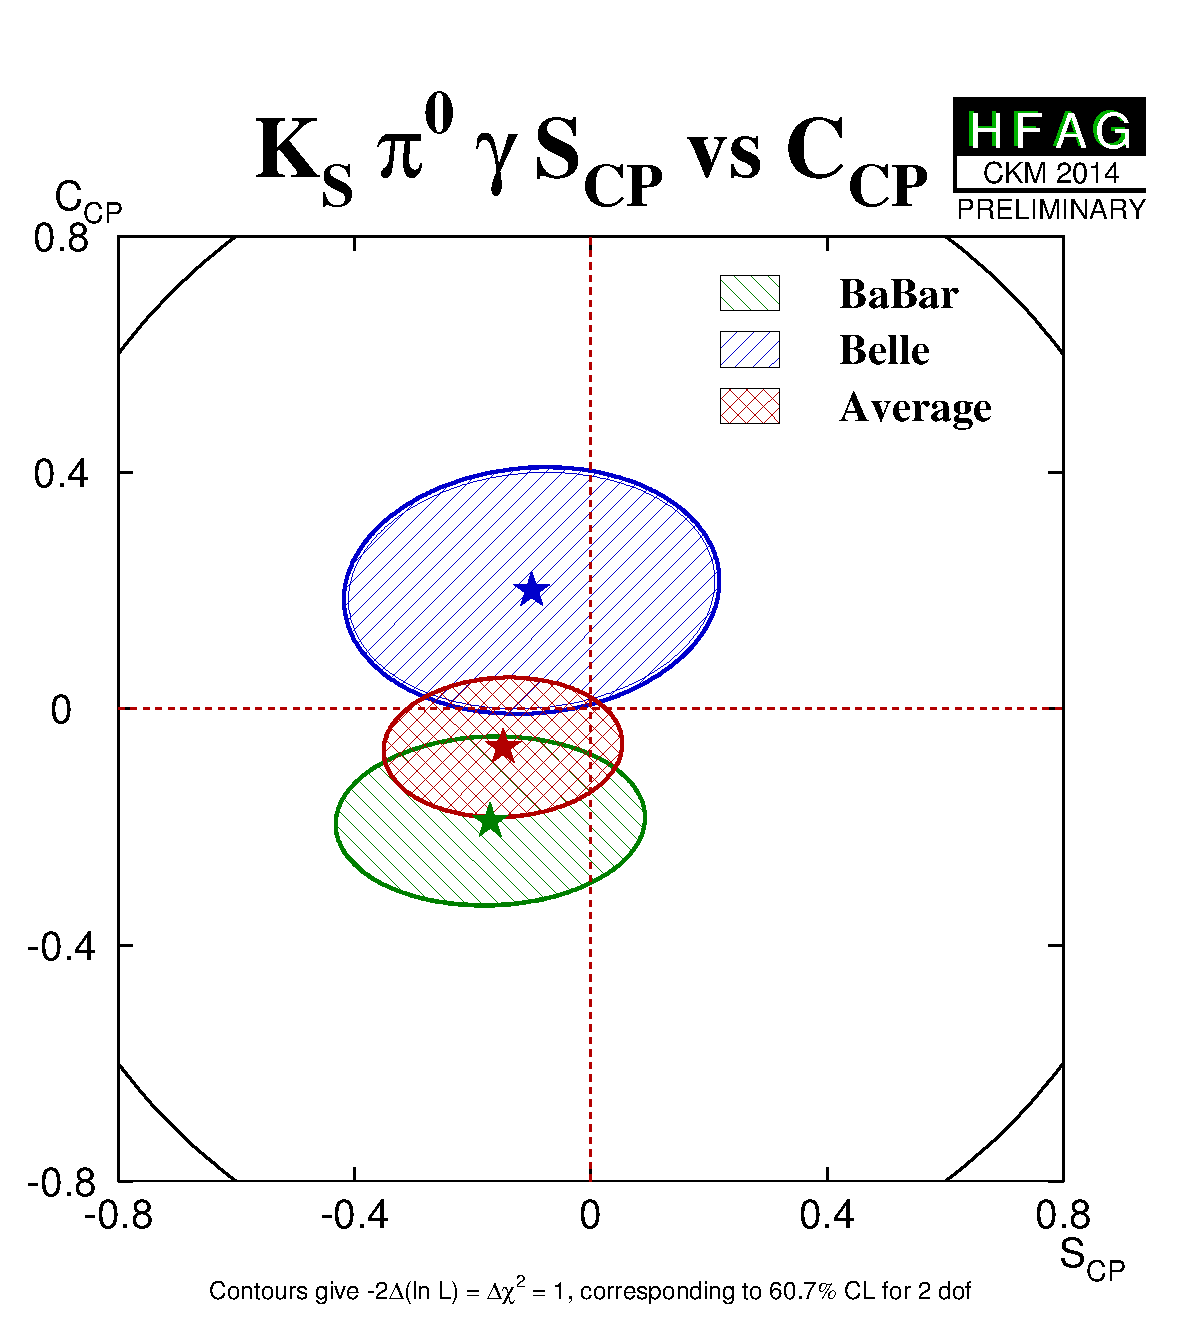
\includegraphics{figures/cp_uta/KSpi0gammaS_CPvsC_CP}
    } \\
    \resizebox{0.33\textwidth}{!}{
      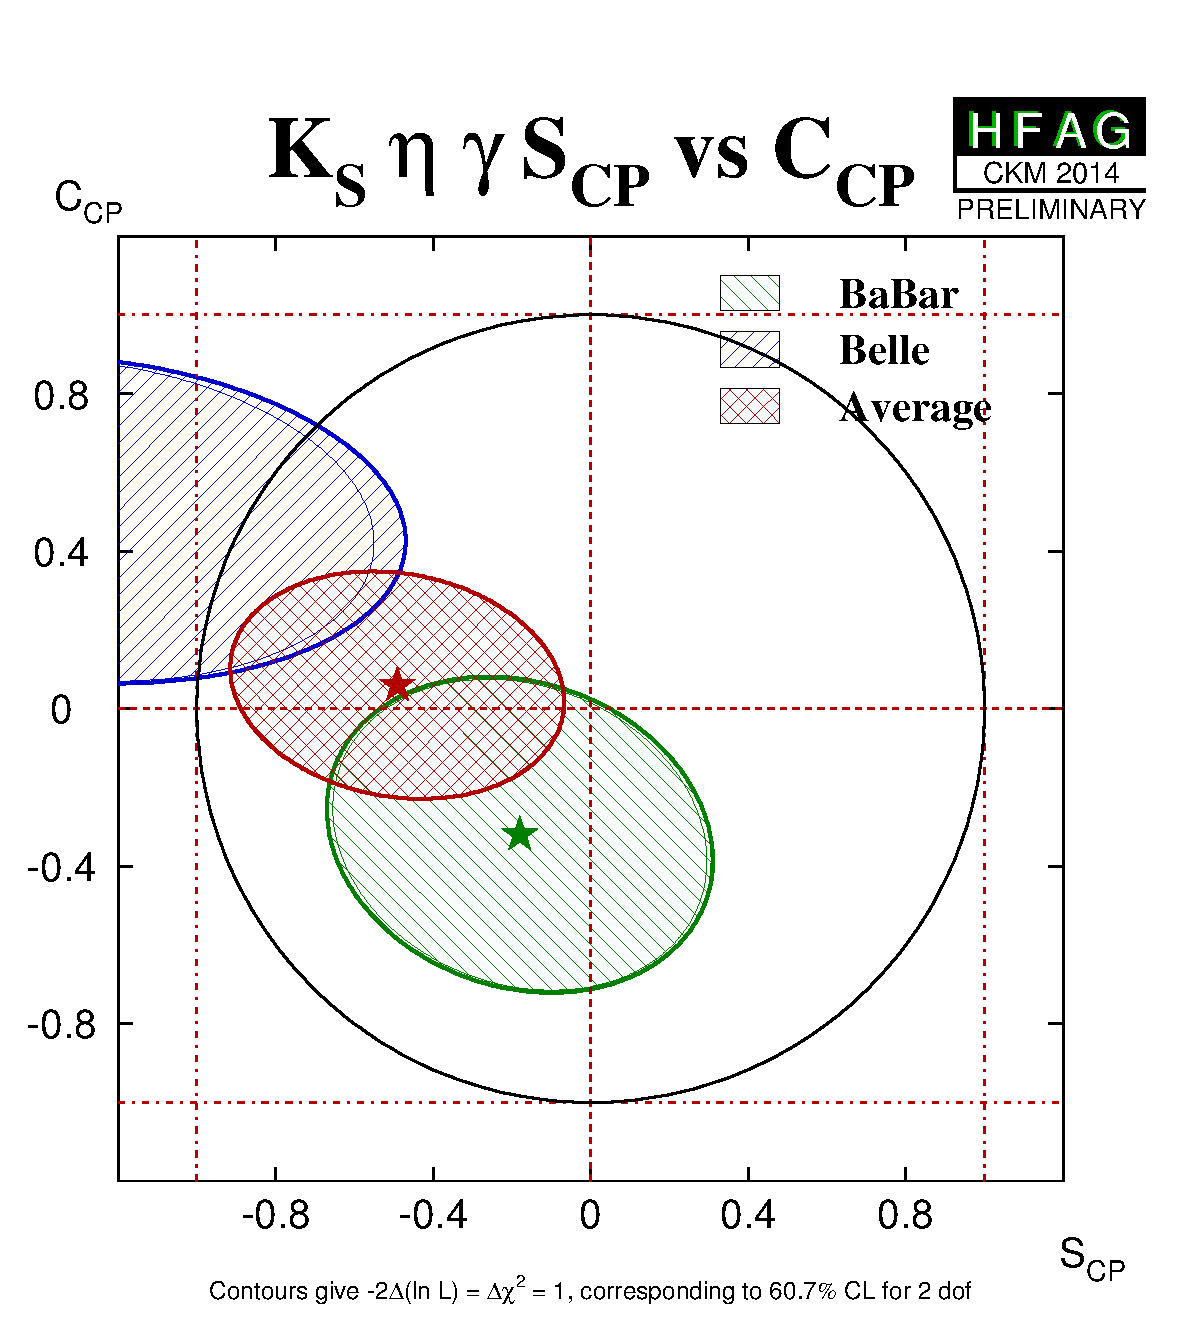
\includegraphics{figures/cp_uta/KSetagammaS_CPvsC_CP}
    }
    \hspace{0.08\textwidth}
    \resizebox{0.33\textwidth}{!}{
      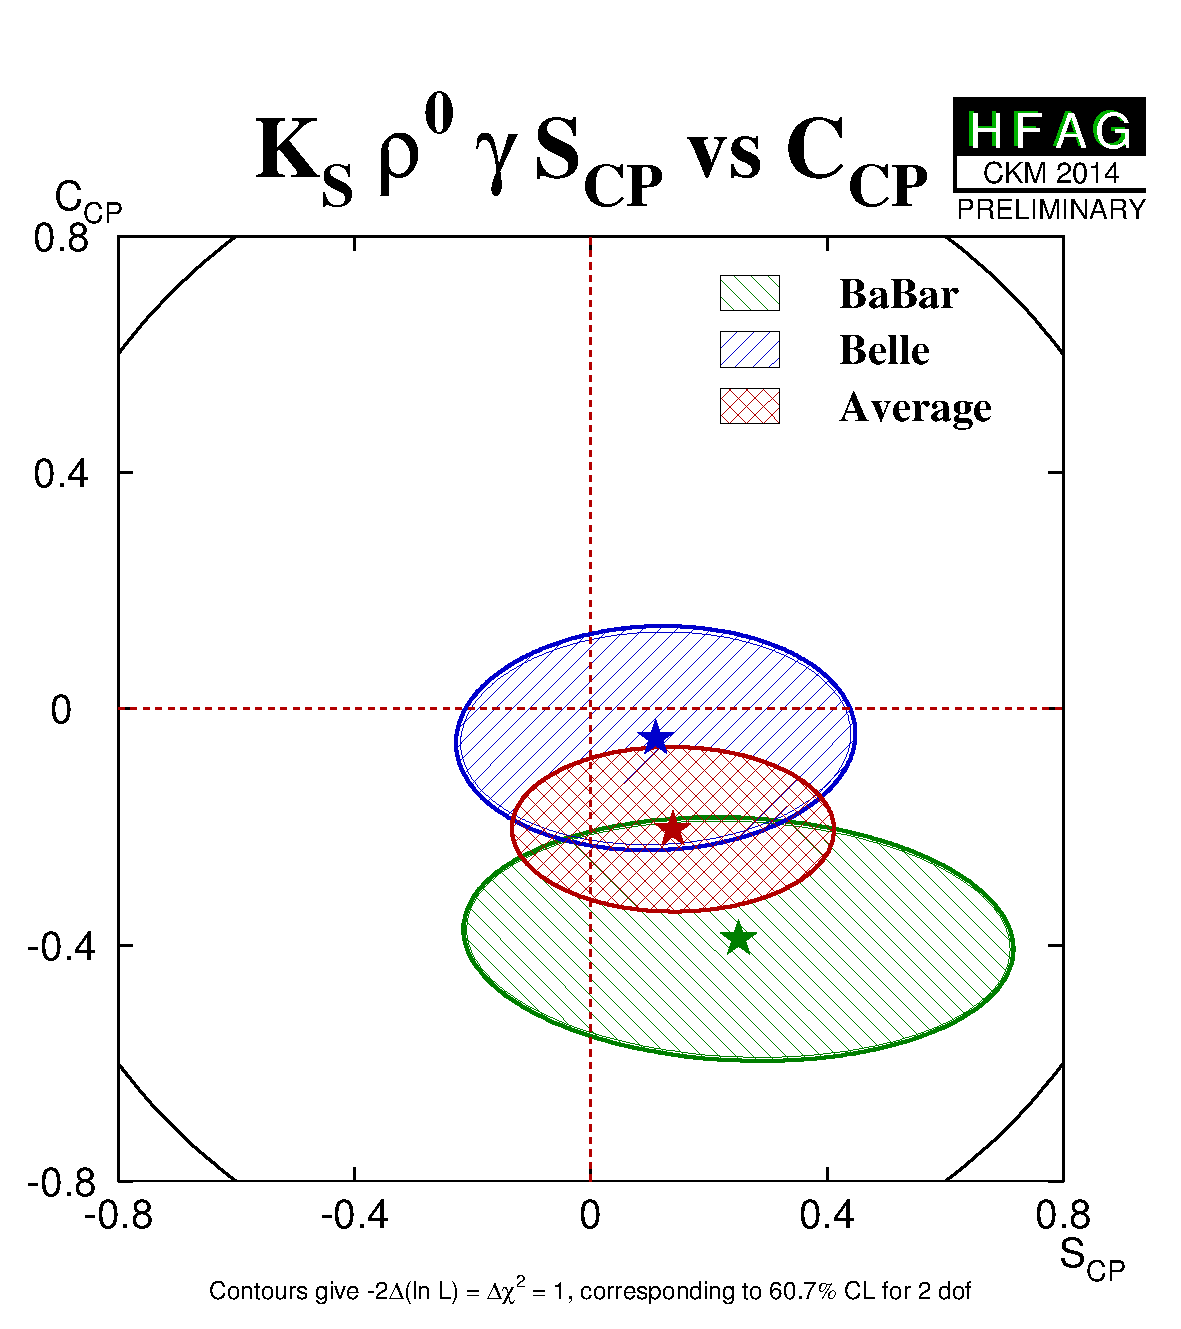
\includegraphics{figures/cp_uta/KSrho0gammaS_CPvsC_CP}
    }
  \end{center}
  \vspace{-0.5cm}
  \caption{
    Averages of four $b \to s\gamma$ dominated channels,
    for which correlated averages are performed,
    in the $S_{\CP}$ \vs\ $C_{\CP}$ plane.
    (Top left) $\Bz \to K^*\gamma$, 
    (top right) $\Bz \to \KS\pi^0\gamma$ (including $K^*\gamma$),
    (bottom left) $\Bz \to \KS\eta\gamma$,
    (bottom right).
  }
  \label{fig:cp_uta:bsg_SvsC}
\end{figure}

%%%%%%%%
%%%
%%% b -> dg
%%%
%%%%%%%%
% \clearpage
\mysubsection{Time-dependent asymmetries in $b \to d\gamma$ transitions
}
\label{sec:cp_uta:bdg}

The formalism for the radiative decays $b \to d\gamma$ is much the same
as that for $b \to s\gamma$ discussed above.
Assuming dominance of the top quark in the loop,
the weak phase in decay should cancel with that from mixing,
so that the mixing-induced \CP\ violation parameter $S_{\CP}$ 
should be very small.
Corrections due to the finite light quark mass are smaller
compared to $b \to s\gamma$, since $m_d < m_s$,
and although QCD corrections may still play a role,
they cannot significantly affect the prediction $S_{b \to d \gamma} \simeq 0$.
Large \CP\ violation effects could, however, be seen through
a non-zero value of $C_{b \to d \gamma}$, 
since the top loop is not the only contribution.

Results using the mode $\Bz \to \rho^0\gamma$ are available from 
\belle\ and are shown in Table~\ref{tab:cp_uta:bdg}.

\begin{table}[htb]
	\begin{center}
		\caption{
			Averages for $\Bz \to \rho^{0} \gamma$.
		}
		\vspace{0.2cm}
		\setlength{\tabcolsep}{0.0pc}
		\begin{tabular*}{\textwidth}{@{\extracolsep{\fill}}lrcccc} \hline
	\mc{2}{l}{Experiment} & $N(B\bar{B})$ & $S_{CP}$ & $C_{CP}$ & Correlation \\
	\hline
	\belle & \cite{Ushiroda:2007jf} & 657M & $-0.83 \pm 0.65 \pm 0.18$ & $0.44 \pm 0.49 \pm 0.14$ & $-0.08$ \\
		\hline
		\end{tabular*}
		\label{tab:cp_uta:bdg}
	\end{center}
\end{table}




%%%%%%%%
%%%
%%% b -> uud
%%%
%%%%%%%%
\clearpage
\mysubsection{Time-dependent $\CP$ asymmetries in $b \to u\bar{u}d$ transitions
}
\label{sec:cp_uta:uud}

The $b \to u \bar u d$ transition can be mediated by either 
a $b \to u$ tree amplitude or a $b \to d$ penguin amplitude.
These transitions can be investigated using 
the time dependence of $\Bz$ decays to final states containing light mesons.
Results are available from both \babar\ and \belle\ for the 
$\CP$ eigenstate ($\etacp = +1$) $\pi^+\pi^-$ final state
and for the vector-vector final state $\rho^+\rho^-$,
which is found to be dominated by the $\CP$-even
longitudinally polarised component
(\babar\ measure $f_{\rm long} = 
0.992 \pm 0.024 \, ^{+0.026}_{-0.013}$~\cite{Aubert:2007nua}
while \belle\ measure $f_{\rm long} = 
0.941 \, ^{+0.034}_{-0.040} \pm 0.030$~\cite{Somov:2006sg}).
\babar\ have also performed a time-dependent analysis of the 
vector-vector final state $\rho^0\rho^0$~\cite{:2008iha},
in which they measure  $f_{\rm long} = 0.70 \pm 0.14 \pm 0.05$;
\belle\ measures a smaller branching fraction than \babar\ for
$\Bz\to\rho^0\rho^0$~\cite{:2008et} with corresponding signal yields too small
to perform time-dependent or angular analyses.
\babar\ have furthermore performed a time-dependent analysis of the 
$\Bz \to a_1^\pm \pi^\mp$ decay~\cite{Aubert:2006gb}; further experimental
input for the extraction of $\alpha$ from this channel is reported in a later
publication~\cite{:2009ii}.

Results, and averages, of time-dependent \CP-violation parameters in 
$b \to u \bar u d$ transitions are listed in Table~\ref{tab:cp_uta:uud}.
The averages for $\pi^+\pi^-$ are shown in Fig.~\ref{fig:cp_uta:uud:pipi},
and those for $\rho^+\rho^-$ are shown in Fig.~\ref{fig:cp_uta:uud:rhorho},
with the averages in the $S_{\CP}$ \vs\ $C_{\CP}$ plane 
shown in Fig.~\ref{fig:cp_uta:uud_SvsC} and
averages of \CP violation parameters in $\Bz \to a_1^\pm \pi^\mp$ decay shown in Fig.~\ref{fig:cp_uta:a1pi}

% \begin{table}[htb]
\begin{sidewaystable}
	\begin{center}
		\caption{
      Averages for $b \to u \bar u d$ modes.
		}
		\vspace{0.2cm}
		\setlength{\tabcolsep}{0.0pc}
		\begin{tabular*}{\textwidth}{@{\extracolsep{\fill}}lrcccc} \hline
	\mc{2}{l}{Experiment} & Sample size & $S_{CP}$ & $C_{CP}$ & Correlation \\
	\hline
      \mc{6}{c}{$\pi^{+} \pi^{-}$} \\
	\babar & \cite{Lees:2012mma} & 467M & $-0.68 \pm 0.10 \pm 0.03$ & $-0.25 \pm 0.08 \pm 0.02$ & $-0.06$ \\
	\belle & \cite{Adachi:2013mae} & 772M & $-0.64 \pm 0.08 \pm 0.03$ & $-0.33 \pm 0.06 \pm 0.03$ & $-0.10$ \\
	LHCb & \cite{Aaij:2013tna} & $1.0 \ {\rm fb}^{-1}$ & $-0.71 \pm 0.13 \pm 0.02$ & $-0.38 \pm 0.15 \pm 0.02$ & $0.38$ \\
%	\hline
	\mc{3}{l}{\bf Average} & $-0.66 \pm 0.06$ & $-0.31 \pm 0.05$ & $0.00$ \\
	\mc{3}{l}{\small Confidence level} & \mc{2}{c}{\small $0.92~(0.1\sigma)$} & \\
		\hline
% 		\end{tabular*}
% 		\label{tab:cp_uta:yyy}
% 	\end{center}
% \end{table}


% \begin{table}[htb]
% 	\begin{center}
% 		\caption{
% 			Averages for $\\rho^{+} \\rho^{-}$.
% 		}
% 		\vspace{0.2cm}
% 		\setlength{\tabcolsep}{0.0pc}
% 		\begin{tabular*}{\textwidth}{@{\extracolsep{\fill}}lrcccc} \hline
% 		\mc{2}{l}{Experiment} & $N(B\bar{B})$ & $S_{CP}$ & $C_{CP}$ & Correlation \\
% 		\hline
      \mc{6}{c}{$\rho^{+} \rho^{-}$} \\
	\babar & \cite{Aubert:2007nua} & $N(B\bar{B}) =$ 387M & $-0.17 \pm 0.20 \,^{+0.05}_{-0.06}$ & $0.01 \pm 0.15 \pm 0.06$ & $-0.04$ \\
	\belle & \cite{Abe:2007ez} & $N(B\bar{B}) =$ 535M & $0.19 \pm 0.30 \pm 0.07$ & $-0.16 \pm 0.21 \pm 0.07$ & $0.10$ \\
%	\hline
	\mc{3}{l}{\bf Average} & $-0.05 \pm 0.17$ & $-0.06 \pm 0.13$ & $0.01$ \\
	\mc{3}{l}{\small Confidence level} & \mc{2}{c}{\small $0.50~(0.7\sigma)$} & \\
		\hline
%		\end{tabular*}
% 		\label{tab:cp_uta:yyy}
% 	\end{center}
% \end{table}

% \begin{table}[htb]
% 	\begin{center}
% 		\caption{
% 			Averages for $\\rho^{0} \\rho^{0}$.
% 		}
% 		\vspace{0.2cm}
% 		\setlength{\tabcolsep}{0.0pc}
% 		\begin{tabular*}{\textwidth}{@{\extracolsep{\fill}}lrcccc} \hline
% 	\mc{2}{l}{Experiment} & $N(B\bar{B})$ & $S_{CP}$ & $C_{CP}$ & Correlation \\
% 	\hline
      \mc{6}{c}{$\rho^{0} \rho^{0}$} \\
	\babar & \cite{:2008iha} & $N(B\bar{B}) =$ 465M & $0.3 \pm 0.7 \pm 0.2$ & $0.2 \pm 0.8 \pm 0.3$ & $-0.04$ \\
%	\hline
% 	\mc{3}{l}{\bf Average} & $0.50 \pm 0.92$ & $0.40 \pm 0.92$ & $0.00$ \\
% 	\mc{3}{l}{\small Confidence level} & \mc{2}{c}{\small $0.xx~(y.y\sigma)$} & \\
 		\hline
 		\end{tabular*}
% 		\label{tab:cp_uta:yyy}
% 	\end{center}
% \end{table}

                \vspace{2ex}

% \begin{table}[htb]
% 	\begin{center}
% 		\caption{
% 			Averages for $a_{1}^{\pm} \\pi^{\mp}$.
% 		}
% 		\vspace{0.2cm}
% 		\setlength{\tabcolsep}{0.0pc}
% make this tabular (not tabular*) and resize down to \textwidth
% change @{\extracolsep{\fill}} to @{\extracolsep{2mm}}
    \resizebox{\textwidth}{!}{
 		\begin{tabular}{@{\extracolsep{2mm}}lrcccccc} \hline
 		\mc{2}{l}{Experiment} & $N(B\bar{B})$ & $A_{CP}^{a_1\pi}$ & $C_{a_1\pi}$ & $S_{a_1\pi}$ & $\Delta C_{a_1\pi}$ & $\Delta S_{a_1\pi}$ \\
 		\hline
      \mc{8}{c}{$a_1^{\pm} \pi^{\mp}$} \\
	\babar & \cite{Aubert:2006gb} & 384M & $-0.07 \pm 0.07 \pm 0.02$ & $-0.10 \pm 0.15 \pm 0.09$ & $0.37 \pm 0.21 \pm 0.07$ & $0.26 \pm 0.15 \pm 0.07$ & $-0.14 \pm 0.21 \pm 0.06$ \\
	\belle & \cite{Dalseno:2012hp} & 772M & $-0.06 \pm 0.05 \pm 0.07$ & $-0.01 \pm 0.11 \pm 0.09$ & $-0.51 \pm 0.14 \pm 0.08$ & $0.54 \pm 0.11 \pm 0.07$ & $-0.09 \pm 0.14 \pm 0.06$ \\ 
 	\hline
	\mc{3}{l}{\bf Average} & $-0.06 \pm 0.06$ & $-0.05 \pm 0.11$ & $-0.20 \pm 0.13$ & $0.43 \pm 0.10$ & $-0.10 \pm 0.12$ \\
	\mc{3}{l}{\small Confidence level} & \mc{5}{c}{\small $0.03~(2.1\sigma)$} \\
        \hline
		\end{tabular}
              }
% 		\label{tab:cp_uta:yyy}
% 	\end{center}
% \end{table}

                \vspace{2ex}

% \begin{table}
% 	\begin{center}
% 		\caption{
% 			Averages for $a_{1}^{\pm} \\pi^{\mp}.DCPV$.
% 		}
% 		\vspace{0.2cm}
% 		\setlength{\tabcolsep}{0.0pc}
		\begin{tabular*}{\textwidth}{@{\extracolsep{\fill}}lrcccc} \hline
		\mc{2}{l}{Experiment} & $N(B\bar{B})$ & ${\cal A}^{-+}_{a_1\pi}$ & ${\cal A}^{+-}_{a_1\pi}$ & Correlation \\
		\hline
	\babar & \cite{Aubert:2006gb} & 384M & $0.07 \pm 0.21 \pm 0.15$ & $0.15 \pm 0.15 \pm 0.07$ & 0.63 \\
	\belle & \cite{Dalseno:2012hp} & 772M & $-0.04 \pm 0.26 \pm 0.19$ & $0.07 \pm 0.08 \pm 0.10$ & 0.61 \\
	\mc{3}{l}{\bf Average} & $0.02 \pm 0.20$ & $0.10 \pm 0.10$ & 0.38 \\
        \mc{3}{l}{\small Confidence level} & \mc{2}{c}{\small $0.92~(0.1\sigma)$} \\
		\hline
		\end{tabular*}

		\label{tab:cp_uta:uud}
	\end{center}
\end{sidewaystable}
% \end{table}




\begin{figure}[htb]
  \begin{center}
    \begin{tabular}{cc}
      \resizebox{0.46\textwidth}{!}{
        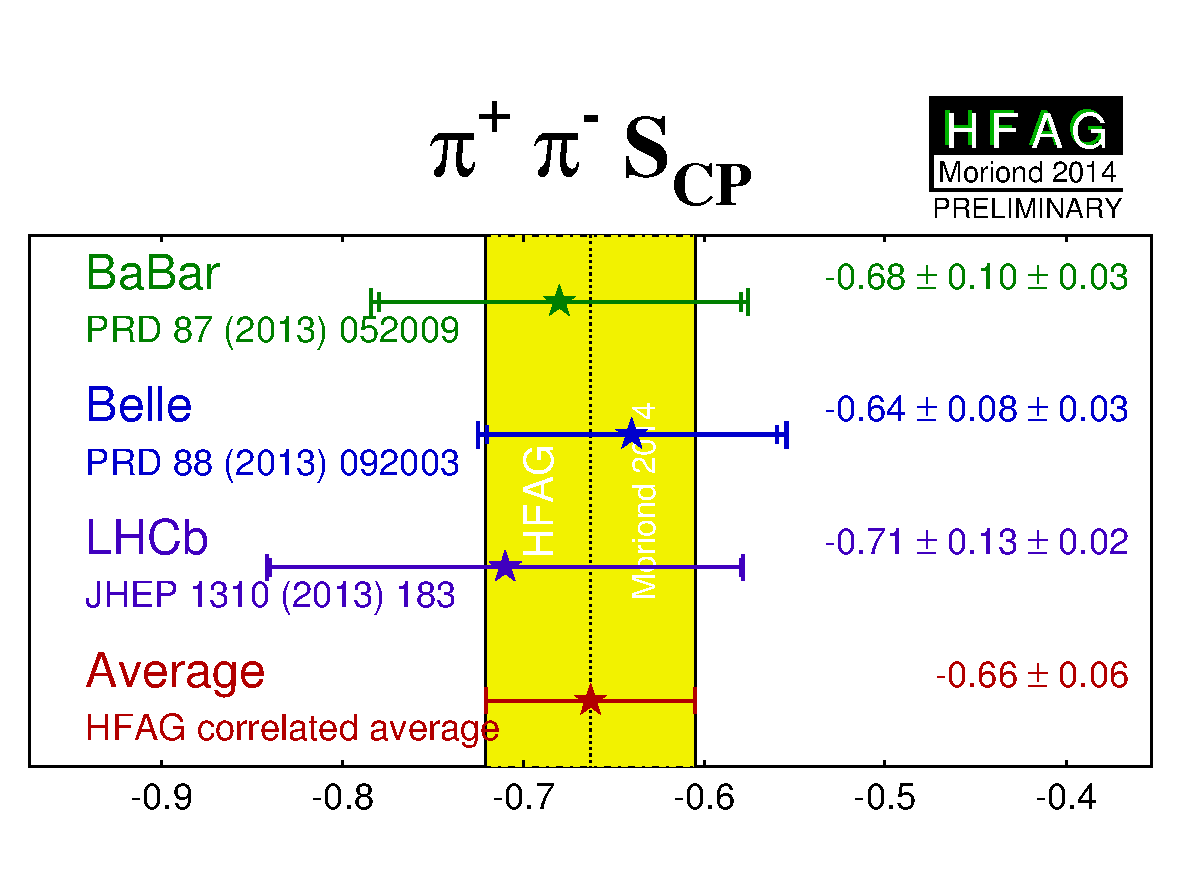
\includegraphics{figures/cp_uta/pi+pi-S_CP}
      }
      &
      \resizebox{0.46\textwidth}{!}{
        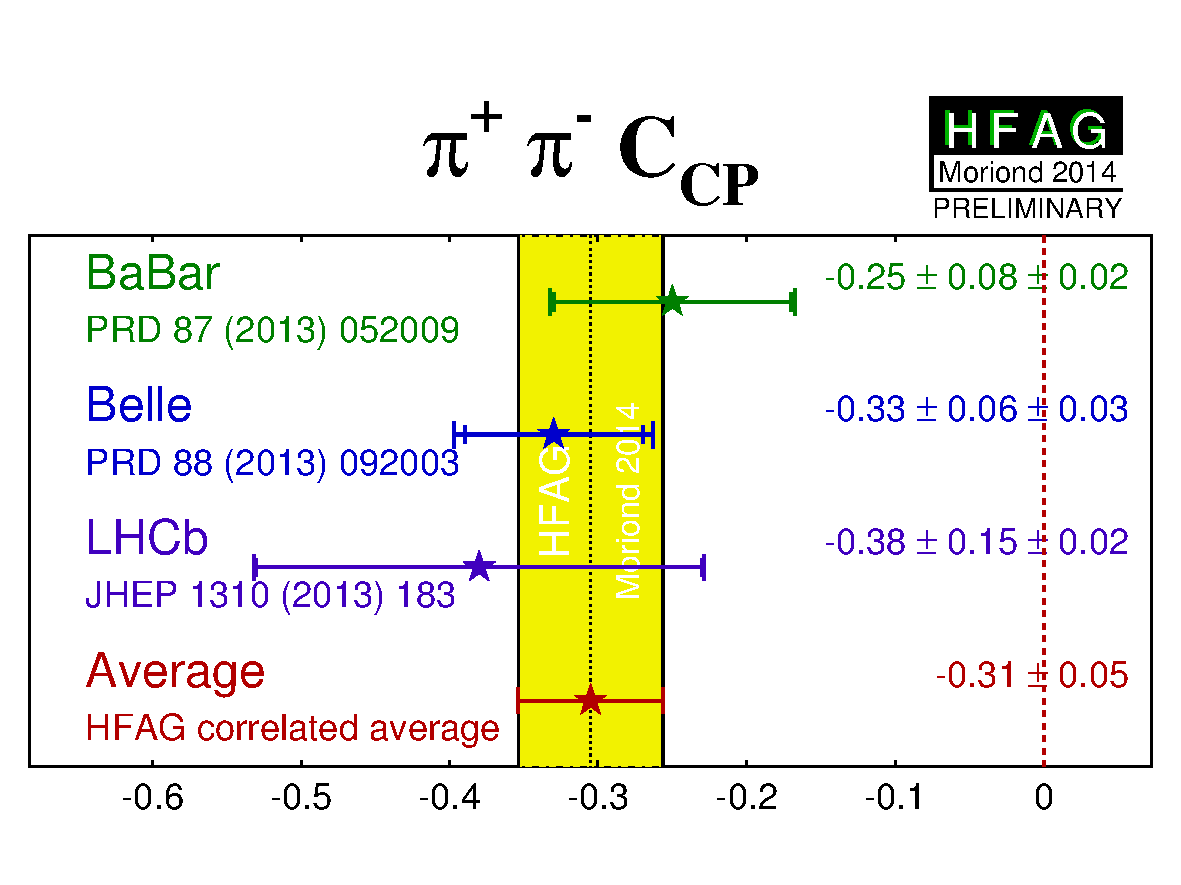
\includegraphics{figures/cp_uta/pi+pi-C_CP}
      }
    \end{tabular}
  \end{center}
  \vspace{-0.8cm}
  \caption{
    Averages of (left) $S_{b \to u\bar u d}$ and (right) $C_{b \to u\bar u d}$
    for the mode $\Bz \to \pi^+\pi^-$.
  }
  \label{fig:cp_uta:uud:pipi}
\end{figure}

\begin{figure}[htb]
  \begin{center}
    \begin{tabular}{cc}
      \resizebox{0.46\textwidth}{!}{
        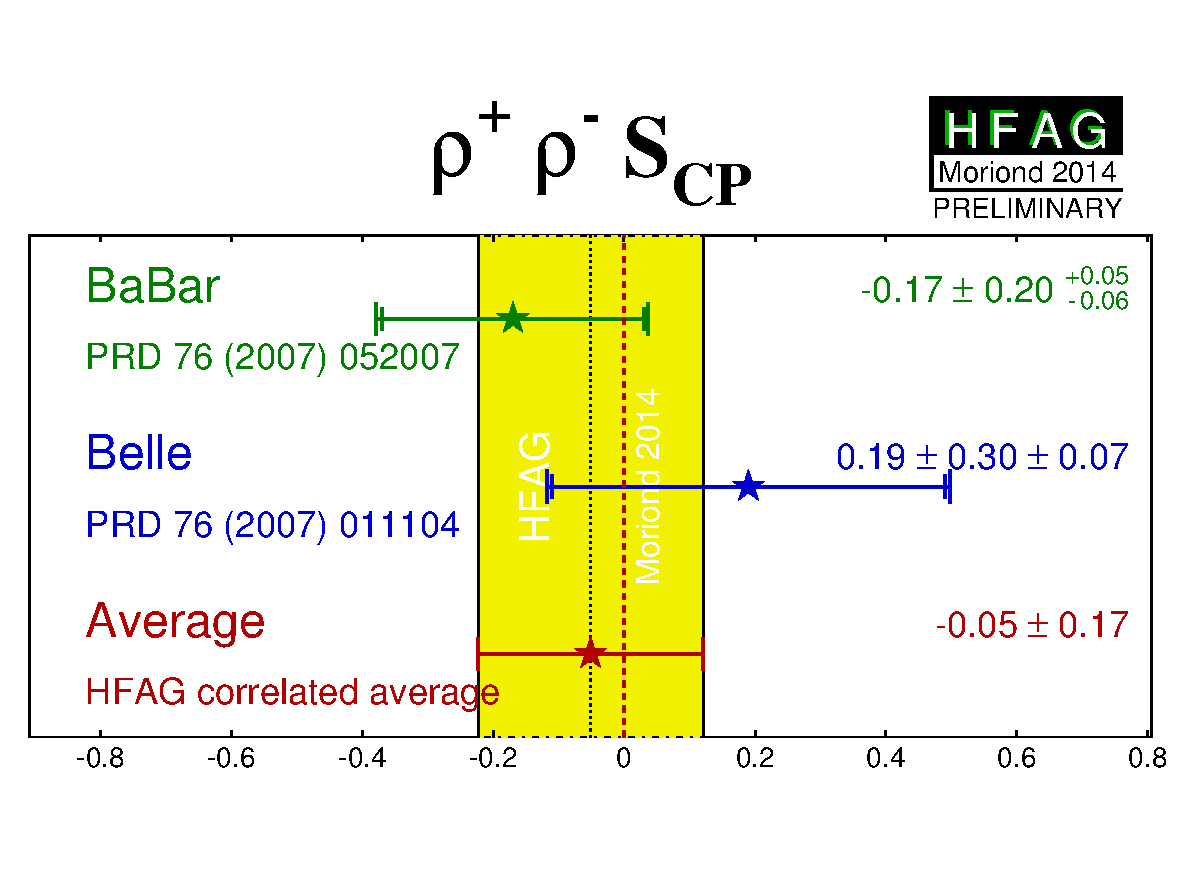
\includegraphics{figures/cp_uta/rho+rho-S_CP}
      }
      &
      \resizebox{0.46\textwidth}{!}{
        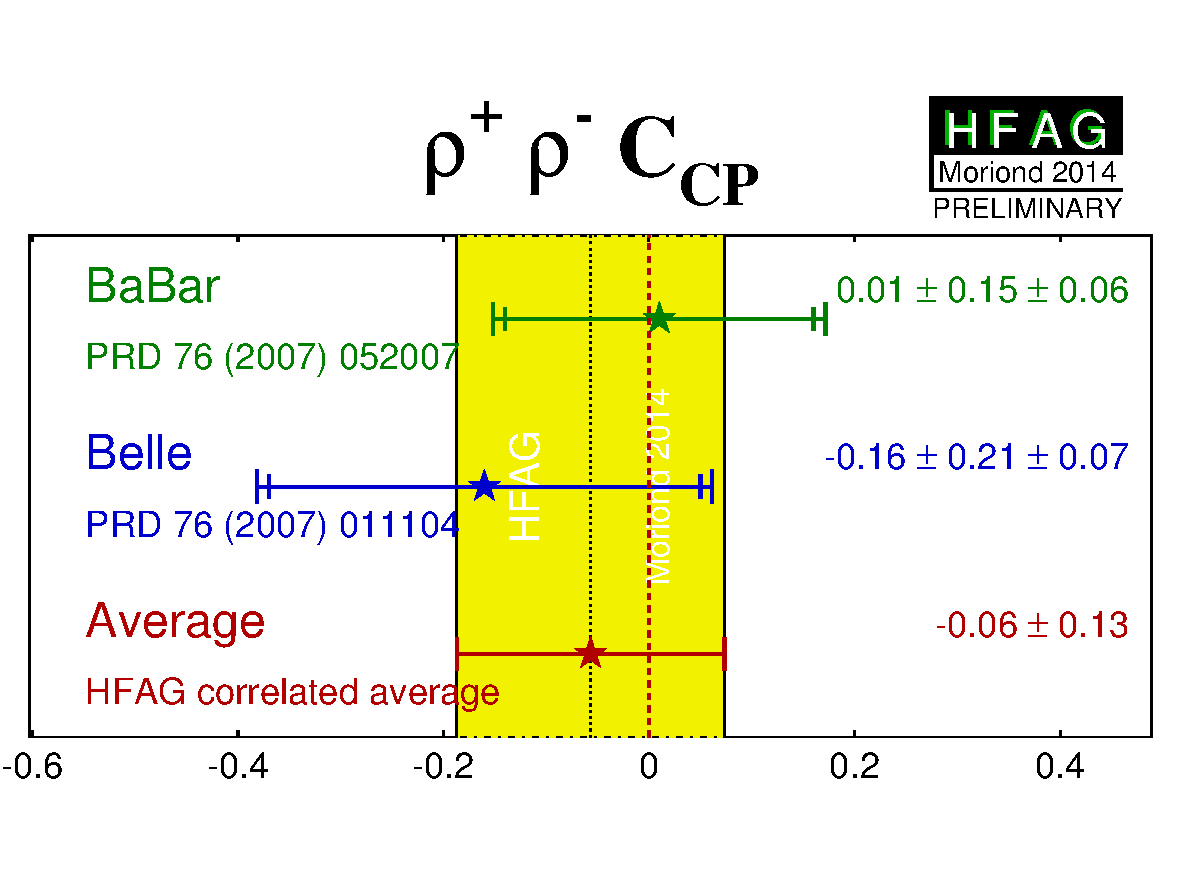
\includegraphics{figures/cp_uta/rho+rho-C_CP}
      }
    \end{tabular}
  \end{center}
  \vspace{-0.8cm}
  \caption{
    Averages of (left) $S_{b \to u\bar u d}$ and (right) $C_{b \to u\bar u d}$
    for the mode $\Bz \to \rho^+\rho^-$.
  }
  \label{fig:cp_uta:uud:rhorho}
\end{figure}

\begin{figure}[htb]
  \begin{center}
    \begin{tabular}{cc}
      \resizebox{0.46\textwidth}{!}{
        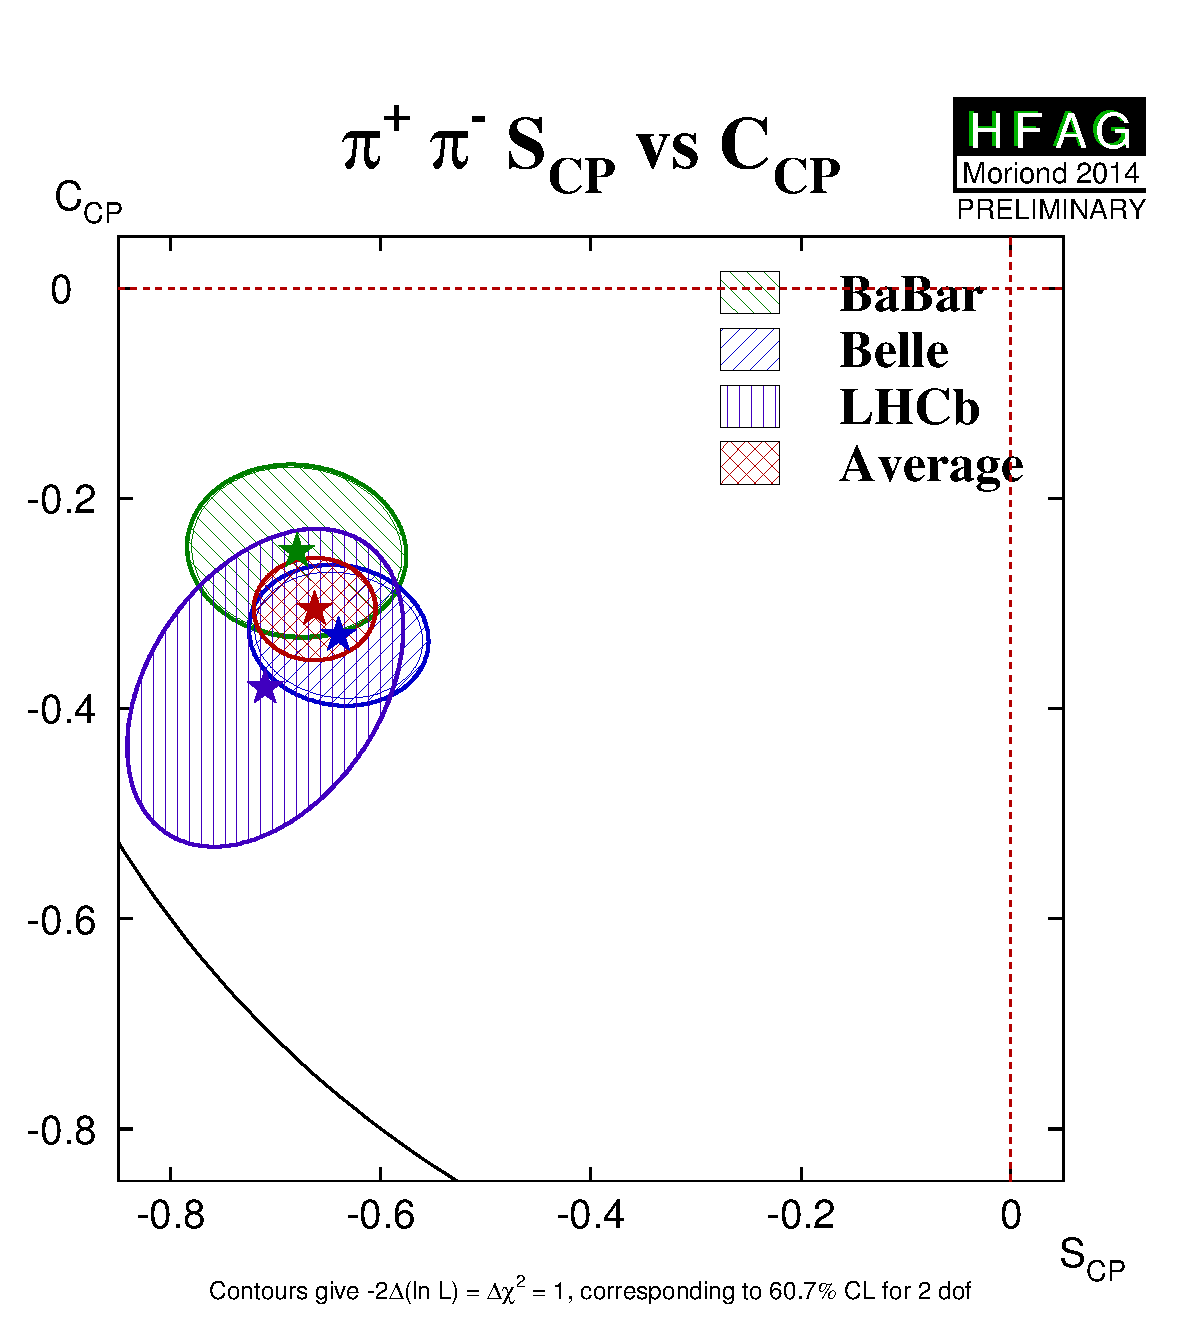
\includegraphics{figures/cp_uta/pi+pi-S_CPvsC_CP}
      }      
      &
      \resizebox{0.46\textwidth}{!}{
        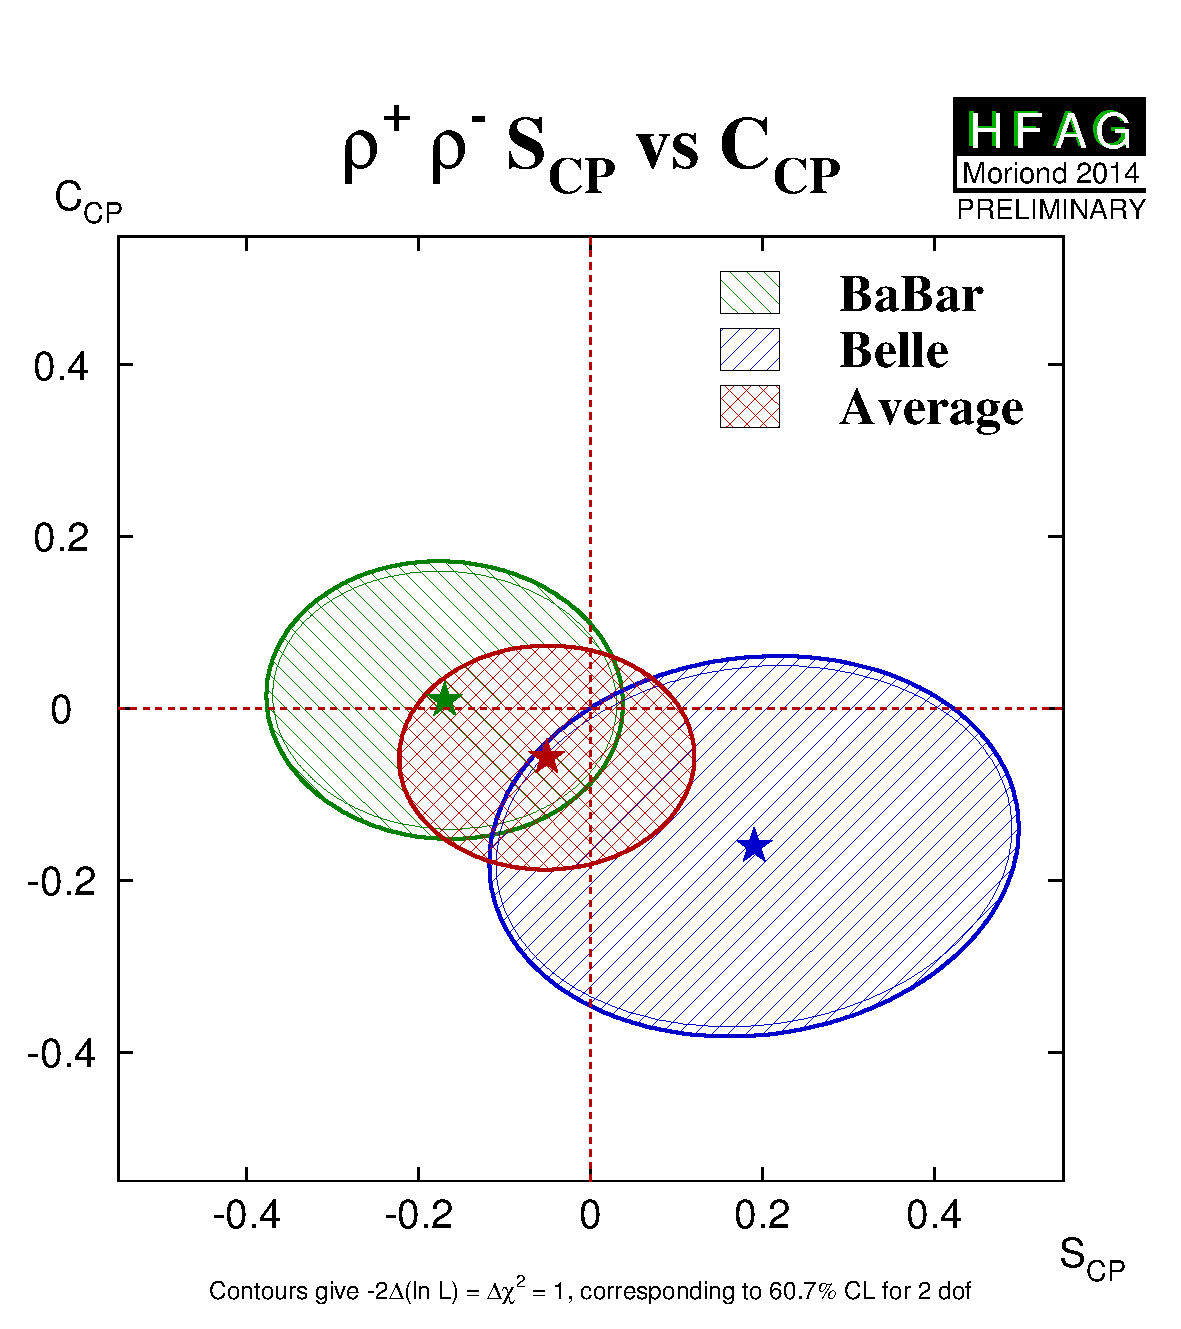
\includegraphics{figures/cp_uta/rho+rho-S_CPvsC_CP}
      }
    \end{tabular}
  \end{center}
  \vspace{-0.8cm}
  \caption{
    Averages of $b \to u\bar u d$ dominated channels,
    for which correlated averages are performed,
    in the $S_{\CP}$ \vs\ $C_{\CP}$ plane.
    (Left) $\Bz \to \pi^+\pi^-$ and (right) $\Bz \to \rho^+\rho^-$.
  }
  \label{fig:cp_uta:uud_SvsC}
\end{figure}

\begin{figure}[htb]
  \begin{center}
    \resizebox{0.46\textwidth}{!}{
      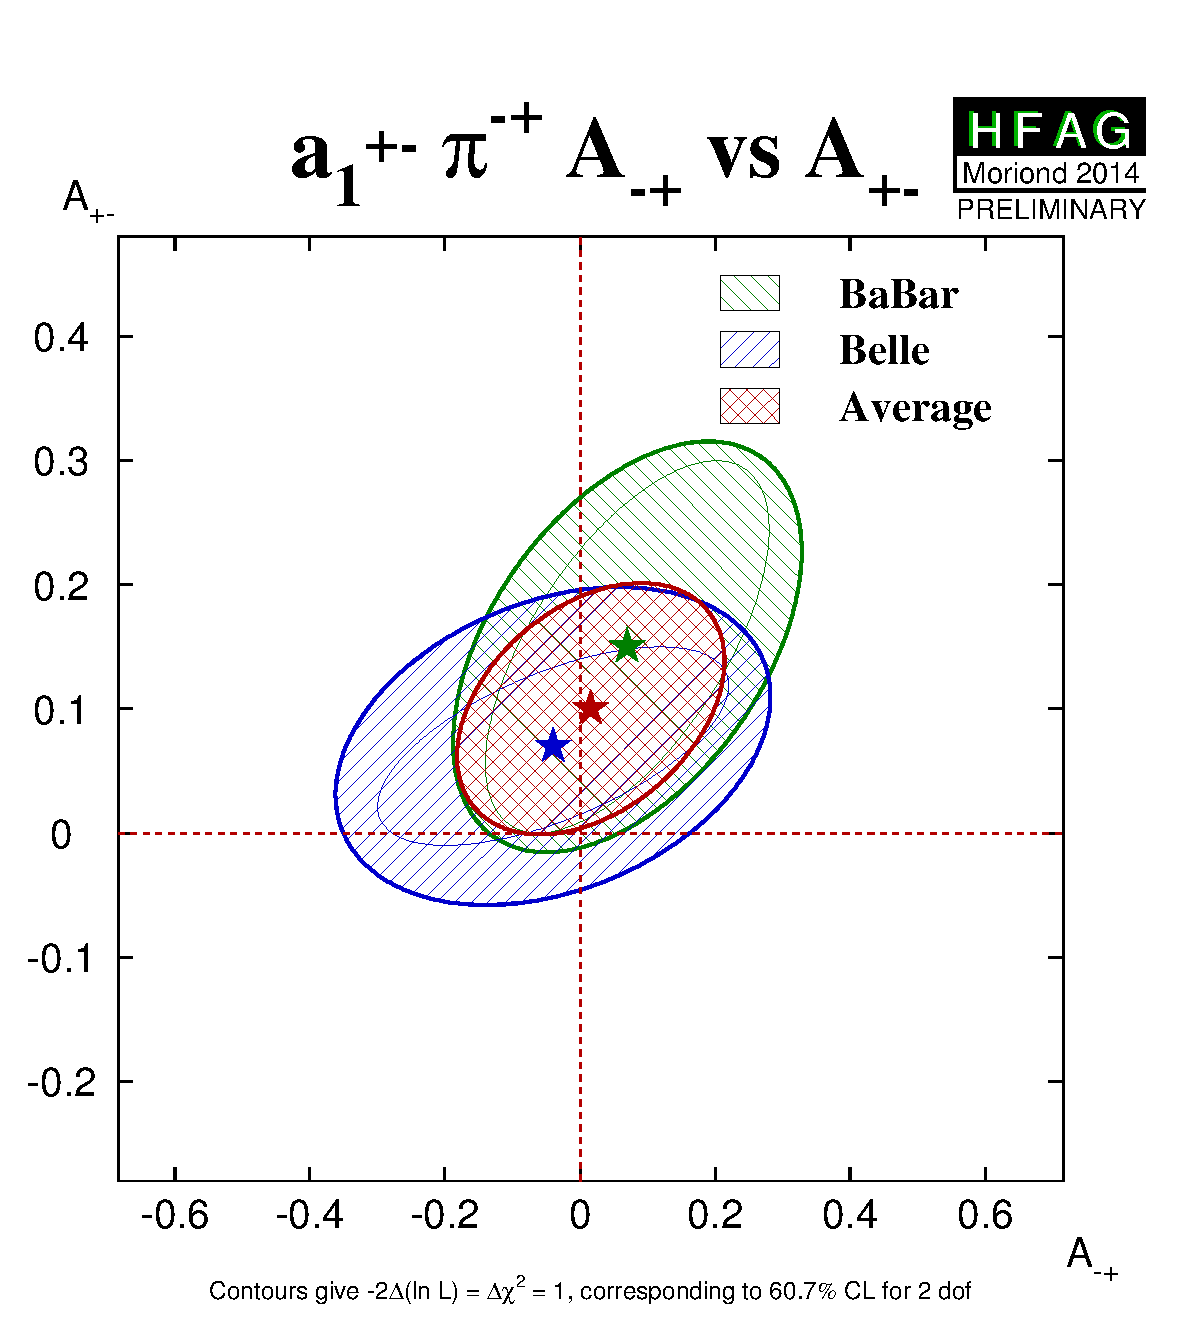
\includegraphics{figures/cp_uta/a1+-pi-+A_-+vsA_+-}
    }
    \vspace{-0.3cm}
    \caption{
      Averages of \CP violation parameters in $\Bz \to a_1^\pm\pi^\mp$ in
      ${\cal A}^{-+}_{a_1\pi}$ \vs\ ${\cal A}^{+-}_{a_1\pi}$ space.
    }
    \label{fig:cp_uta:a1pi}
  \end{center}
\end{figure}

If the penguin contribution is negligible, 
the time-dependent parameters for $\Bz \to \pi^+\pi^-$ 
and $\Bz \to \rho^+\rho^-$ are given by
$S_{b \to u\bar u d} = \etacp \sin(2\alpha)$ and
$C_{b \to u\bar u d} = 0$.
In the presence of the penguin contribution, 
$\CP$ violation in decay may arise, 
and there is no straightforward interpretation 
of $S_{b \to u\bar u d}$ and $C_{b \to u\bar u d}$.
An isospin analysis~\cite{Gronau:1990ka} 
can be used to disentangle the contributions and extract $\alpha$.

For the non-$\CP$ eigenstate $\rho^{\pm}\pi^{\mp}$, 
both \babar~\cite{Aubert:2007jn} 
and \belle~\cite{Kusaka:2007dv,:2007mj} have performed 
time-dependent Dalitz plot (DP) analyses
of the $\pi^+\pi^-\pi^0$ final state~\cite{Snyder:1993mx};
such analyses allow direct measurements of the phases.
Both experiments have measured the $U$ and $I$ parameters discussed in 
Sec.~\ref{sec:cp_uta:notations:dalitz:pipipi0} and defined in 
Table~\ref{tab:cp_uta:pipipi0:uandi}.
We have performed a full correlated average of these parameters,
the results of which are summarised in Fig.~\ref{fig:cp_uta:uud:uandi}.

\begin{figure}[htb]
  \begin{center}
    \begin{tabular}{cc}
      \resizebox{0.46\textwidth}{!}{
        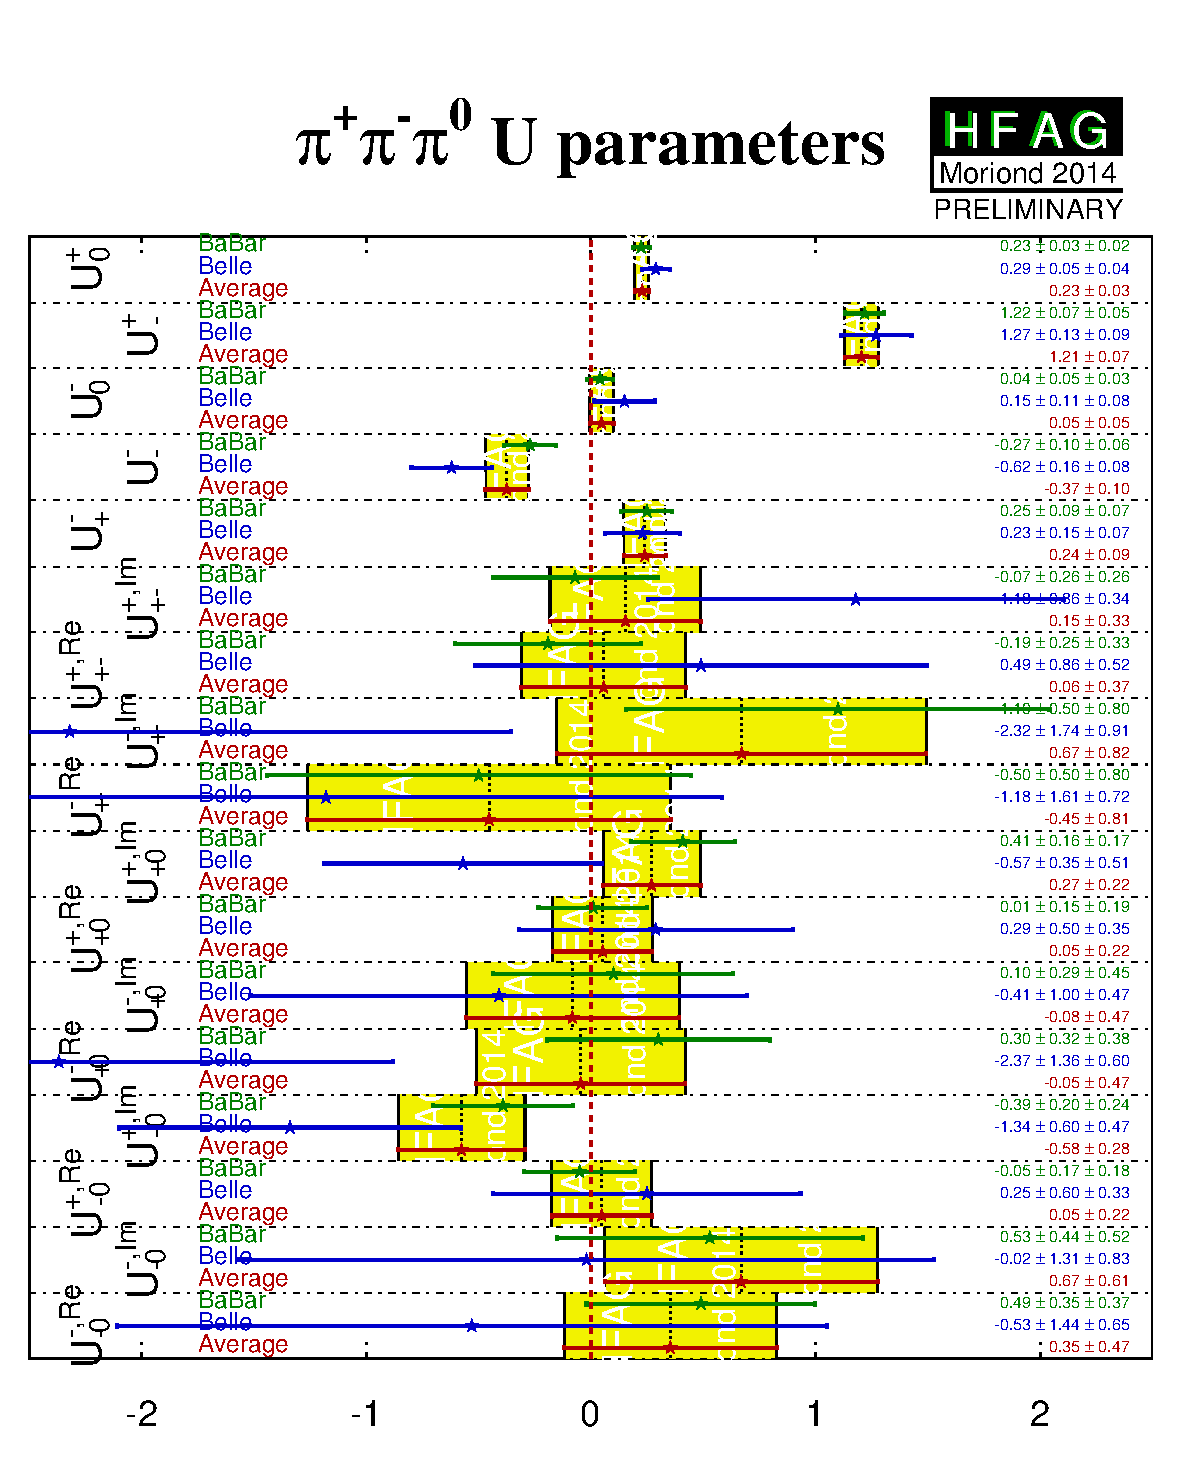
\includegraphics{figures/cp_uta/pi+pi-pi0_U}
      }
      &
      \resizebox{0.46\textwidth}{!}{
        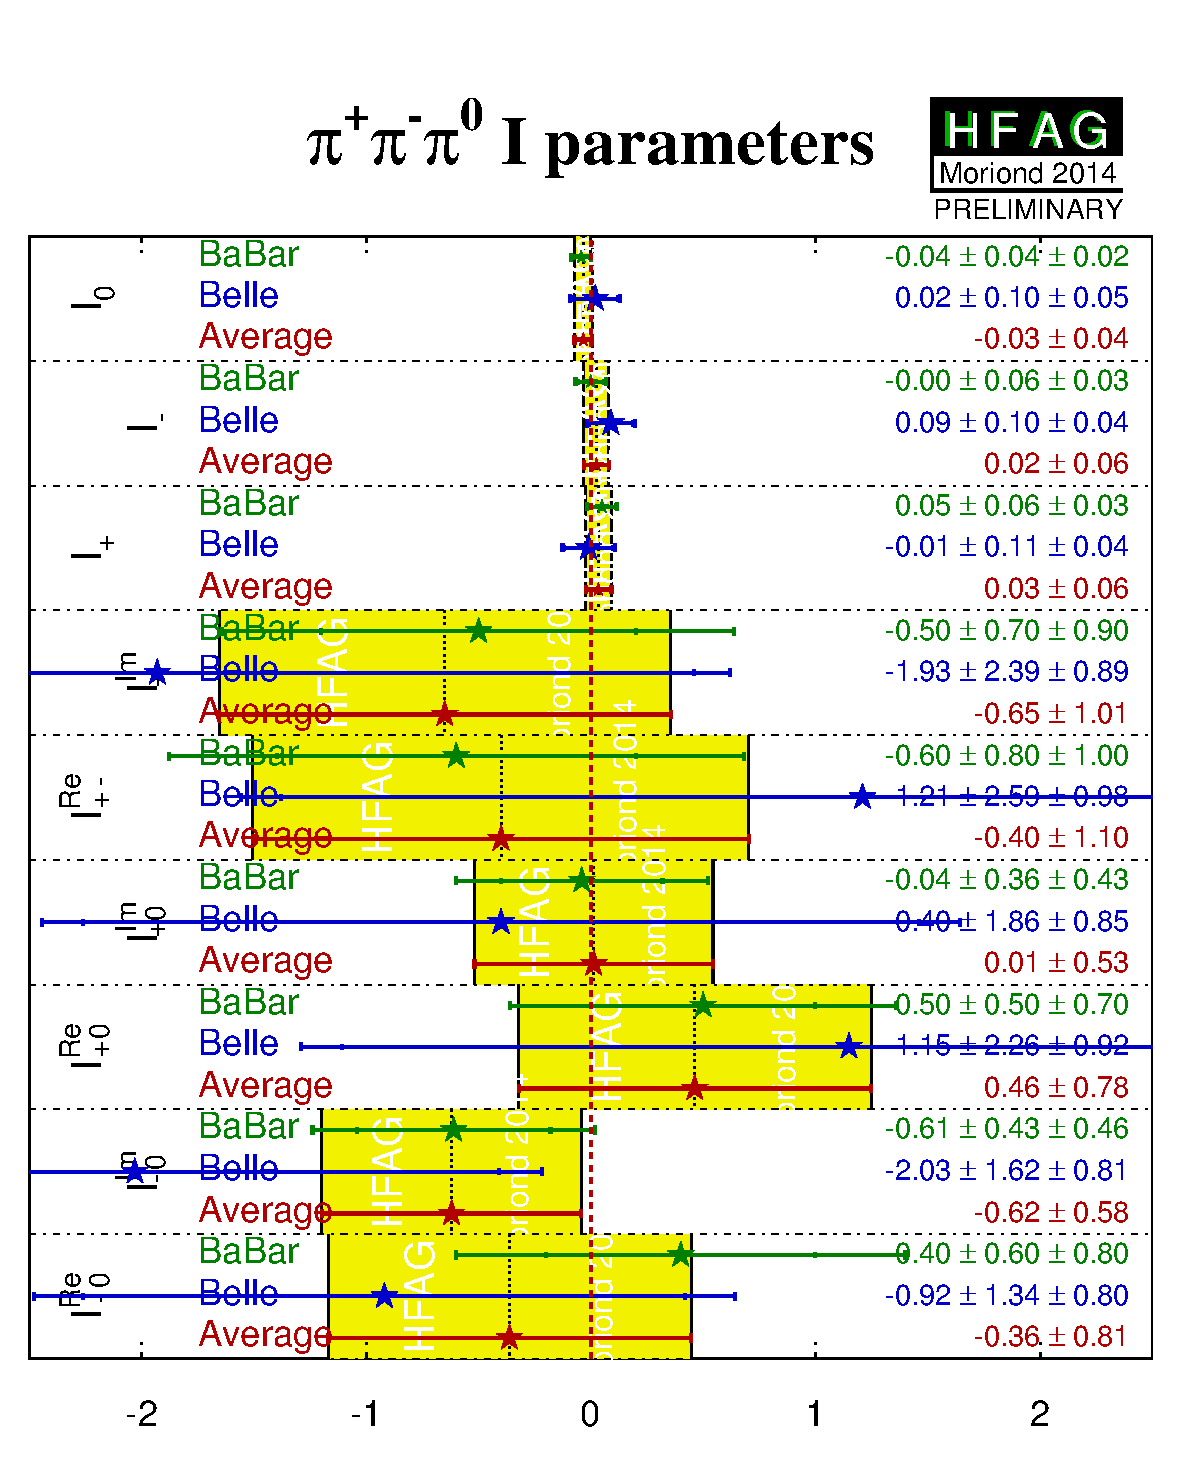
\includegraphics{figures/cp_uta/pi+pi-pi0_I}
      }
    \end{tabular}
  \end{center}
  \vspace{-0.8cm}
  \caption{
    Summary of the $U$ and $I$ parameters measured in the 
    time-dependent $\Bz \to \pi^+\pi^-\pi^0$ Dalitz plot analysis.
  }
  \label{fig:cp_uta:uud:uandi}
\end{figure}

Both experiments have also extracted the Q2B parameters.
We have performed a full correlated average of these parameters,
which is equivalent to determining the values from the 
averaged $U$ and $I$ parameters.
The results are shown in Table.~\ref{tab:cp_uta:uud:rhopi_q2b}.
Averages of the $\Bz \to \rho^0\pi^0$ Q2B parameters are shown in 
Figs.~\ref{fig:cp_uta:uud:rho0pi0} and~\ref{fig:cp_uta:uud:rho0pi0_SvsC}.

% \begin{table}[htb]
\begin{sidewaystable}
	\begin{center}
		\caption{
                  Averages of quasi-two-body parameters extracted
                  from time-dependent Dalitz plot analysis of 
                  $\Bz \to \pi^+\pi^-\pi^0$.
%			Averages for $\\rho^{\pm}\\pi^{\mp}$.
		}
		\vspace{0.2cm}
		\setlength{\tabcolsep}{0.0pc}
% make this tabular (not tabular*) and resize down to \textwidth
% change @{\extracolsep{\fill}} to @{\extracolsep{2mm}}
    \resizebox{\textwidth}{!}{
		\begin{tabular}{@{\extracolsep{2mm}}lrcccccc} \hline
		\mc{2}{l}{Experiment} & $N(B\bar{B})$ & ${\cal A}_{CP}^{\rho\pi}$ & $C_{\rho\pi}$ & $S_{\rho\pi}$ & $\Delta C_{\rho\pi}$ & $\Delta S_{\rho\pi}$ \\
	\hline
	\babar & \cite{Lees:2013nwa} & 471M & $-0.10 \pm 0.03 \pm 0.02$ & $0.02 \pm 0.06 \pm 0.04$ & $0.05 \pm 0.08 \pm 0.03$ & $0.23 \pm 0.06 \pm 0.05$ & $0.05 \pm 0.08 \pm 0.04$ \\
	\belle & \cite{Kusaka:2007dv,:2007mj} & 449M & $-0.12 \pm 0.05 \pm 0.04$ & $-0.13 \pm 0.09 \pm 0.05$ & $0.06 \pm 0.13 \pm 0.05$ & $0.36 \pm 0.10 \pm 0.05$ & $-0.08 \pm 0.13 \pm 0.05$ \\
%	\hline
	\mc{3}{l}{\bf Average} & $-0.11 \pm 0.03$ & $-0.03 \pm 0.06$ & $0.06 \pm 0.07$ & $0.27 \pm 0.06$ & $0.01 \pm 0.08$ \\
	\mc{3}{l}{\small Confidence level} & \mc{5}{c}{\small $0.63~(0.5\sigma)$} \\
        \hline
		\end{tabular}
              }
% 		\label{tab:cp_uta:yyy}
% 	\end{center}
% \end{table}

                \vspace{2ex}

% \begin{table}
% 	\begin{center}
% 		\caption{
% 			Averages for $\\rho^{\pm}\\pi^{\mp}.DCPV$.
% 		}
% 		\vspace{0.2cm}
% 		\setlength{\tabcolsep}{0.0pc}
		\begin{tabular*}{\textwidth}{@{\extracolsep{\fill}}lrcccc} \hline
		\mc{2}{l}{Experiment} & $N(B\bar{B})$ & ${\cal A}^{-+}_{\rho\pi}$ & ${\cal A}^{+-}_{\rho\pi}$ & Correlation \\
		\hline
	\babar & \cite{Lees:2013nwa} & 471M & $-0.12 \pm 0.08 \,^{+0.04}_{-0.05}$ & $0.09 \,^{+0.05}_{-0.06} \pm 0.04$ & $0.55$ \\
	\belle & \cite{Kusaka:2007dv,:2007mj} & 449M & $0.08 \pm 0.16 \pm 0.11$ & $0.21 \pm 0.08 \pm 0.04$ & $0.47$ \\
%	\hline
	\mc{3}{l}{\bf Average} & $-0.08 \pm 0.08$ & $0.13 \pm 0.05$ & $0.37$ \\
        \mc{3}{l}{\small Confidence level} & \mc{2}{c}{\small $0.47~(0.7\sigma)$} \\
		\hline
		\end{tabular*}
% 		\label{tab:cp_uta:yyy}
% 	\end{center}
% \end{table}

                \vspace{2ex}

% \begin{table}
% 	\begin{center}
% 		\caption{
% 			Averages for $\\rho^{0}\\pi^{0}$.
% 		}
% 		\vspace{0.2cm}
% 		\setlength{\tabcolsep}{0.0pc}
		\begin{tabular*}{\textwidth}{@{\extracolsep{\fill}}lrcccc} \hline
		\mc{2}{l}{Experiment} & $N(B\bar{B})$ & $C_{\rho^0\pi^0}$ & $S_{\rho^0\pi^0}$ & Correlation \\
		\hline
	\babar & \cite{Lees:2013nwa} & 471M & $0.19 \pm 0.23 \pm 0.15$ & $-0.37 \pm 0.34 \pm 0.20$ & $0.00$ \\
	\belle & \cite{Kusaka:2007dv,:2007mj} & 449M & $0.49 \pm 0.36 \pm 0.28$ & $0.17 \pm 0.57 \pm 0.35$ & $0.08$ \\
%	\hline
	\mc{3}{l}{\bf Average} & $0.27 \pm 0.24$ & $-0.23 \pm 0.34$ & $0.02$ \\
	\mc{3}{l}{\small Confidence level} & \mc{2}{c}{\small $0.68~(0.4\sigma)$} \\
		\hline
		\end{tabular*}
		\label{tab:cp_uta:uud:rhopi_q2b}
	\end{center}
\end{sidewaystable}
% \end{table}




\begin{figure}[htb]
  \begin{center}
    \begin{tabular}{cc}
      \resizebox{0.46\textwidth}{!}{
        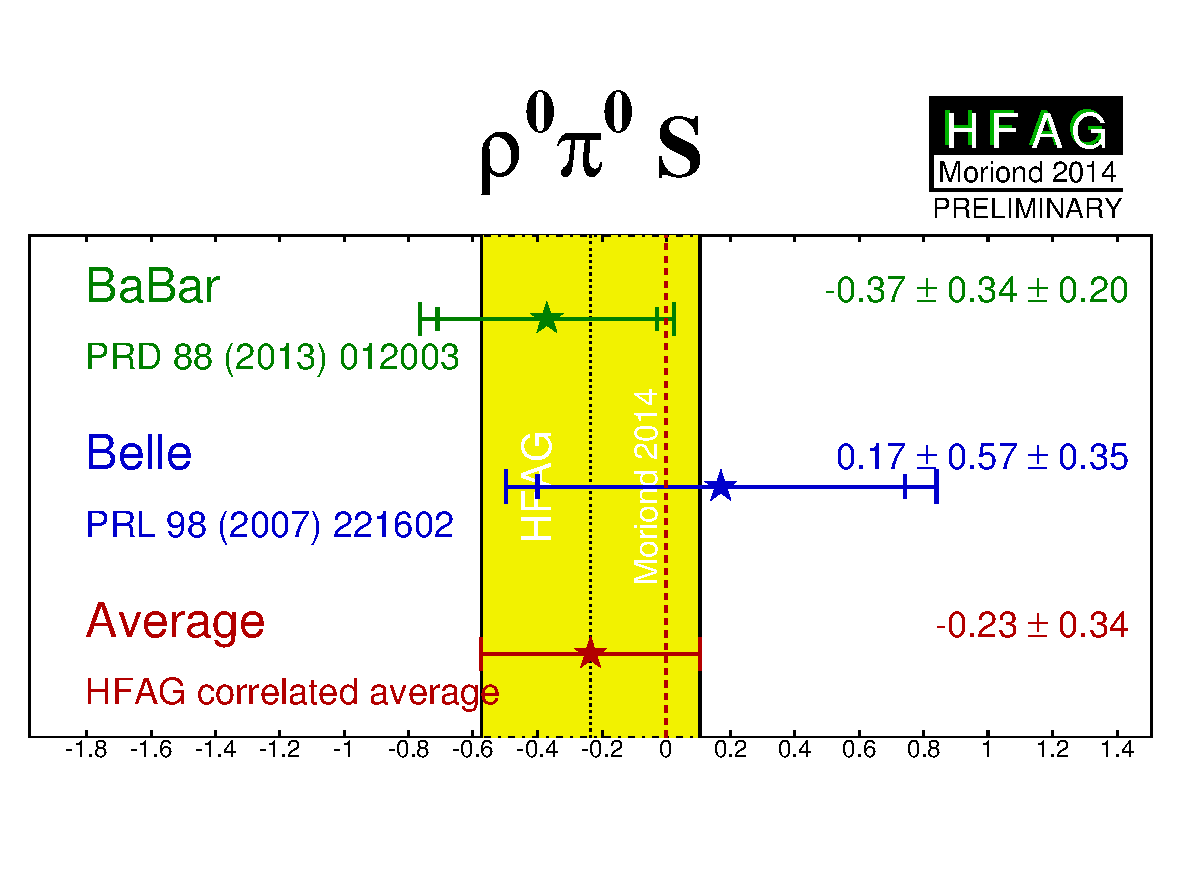
\includegraphics{figures/cp_uta/rho0pi0S}
      }
      &
      \resizebox{0.46\textwidth}{!}{
        \includegraphics{figures/cp_uta/rho0pi0C}
      }
    \end{tabular}
  \end{center}
  \vspace{-0.8cm}
  \caption{
    Averages of (left) $S_{b \to u\bar u d}$ and (right) $C_{b \to u\bar u d}$
    for the mode $\Bz \to \rho^0\pi^0$.
  }
  \label{fig:cp_uta:uud:rho0pi0}
\end{figure}

\begin{figure}[htb]
  \begin{center}
    \resizebox{0.46\textwidth}{!}{
      \includegraphics{figures/cp_uta/rho0pi0CvsS}
    }      
  \end{center}
  \vspace{-0.8cm}
  \caption{
    Averages of $b \to u\bar u d$ dominated channels,
    for the mode $\Bz \to \rho^0\pi^0$
    in the $S_{\CP}$ \vs\ $C_{\CP}$ plane.
  }
  \label{fig:cp_uta:uud:rho0pi0_SvsC}
\end{figure}

With the notation described in Sec.~\ref{sec:cp_uta:notations}
(Eq.~(\ref{eq:cp_uta:non-cp-s_and_deltas})), 
the time-dependent parameters for the Q2B $\Bz \to \rho^\pm\pi^\mp$ analysis are,
neglecting penguin contributions, given by
\begin{equation}
  S_{\rho\pi} = 
  \sqrt{1 - \left(\frac{\Delta C}{2}\right)^2}\sin(2\alpha)\cos(\delta)
  \ , \ \ \ 
  \Delta S_{\rho\pi} = 
  \sqrt{1 - \left(\frac{\Delta C}{2}\right)^2}\cos(2\alpha)\sin(\delta)
\end{equation} 
and $C_{\rho\pi} = {\cal A}_{\CP}^{\rho\pi} = 0$,
where $\delta=\arg(A_{-+}A^*_{+-})$ is the strong phase difference 
between the $\rho^-\pi^+$ and $\rho^+\pi^-$ decay amplitudes.
In the presence of the penguin contribution, there is no straightforward 
interpretation of the Q2B observables in the $\Bz \to \rho^\pm\pi^\mp$ system
in terms of CKM parameters.
However, $\CP$ violation in decay may arise,
resulting in either or both of $C_{\rho\pi} \neq 0$ and ${\cal A}_{\CP}^{\rho\pi} \neq 0$.
Equivalently,
$\CP$ violation in decay may be seen by either of
the decay-type-specific observables ${\cal A}^{+-}_{\rho\pi}$ 
and ${\cal A}^{-+}_{\rho\pi}$, defined in Eq.~(\ref{eq:cp_uta:non-cp-directcp}), 
deviating from zero.
Results and averages for these parameters
are also given in Table~\ref{tab:cp_uta:uud:rhopi_q2b}.
Averages of $\CP$ violation parameters in $\Bz \to \rho^\pm\pi^\mp$ decays
are shown in Fig.~\ref{fig:cp_uta:uud:rhopi-dircp},
both in 
${\cal A}^{\rho\pi}_{\CP}$ \vs\ $C_{\rho\pi}$ space and in 
${\cal A}^{-+}_{\rho\pi}$ \vs\ ${\cal A}^{+-}_{\rho\pi}$ space.

\begin{figure}[htb]
  \begin{center}
    \resizebox{0.46\textwidth}{!}{
      \includegraphics{figures/cp_uta/rho+-pi-+A_CPvsC}
    }
    \hfill
    \resizebox{0.46\textwidth}{!}{
      \includegraphics{figures/cp_uta/rho+-pi-+DCPVA_-+vsA_+-}
    }
  \end{center}
  \vspace{-0.8cm}
  \caption{
    $\CP$ violation in $\Bz\to\rho^\pm\pi^\mp$ decays.
    (Left) ${\cal A}^{\rho\pi}_{\CP}$ \vs\ $C_{\rho\pi}$ space,
    (right) ${\cal A}^{-+}_{\rho\pi}$ \vs\ ${\cal A}^{+-}_{\rho\pi}$ space.
  }
  \label{fig:cp_uta:uud:rhopi-dircp}
\end{figure}

%% straightforward interpretation
Some difference is seen between the 
\babar\ and \belle\ measurements in the $\pi^+\pi^-$ system.
The confidence level of the average is $0.034$,
which corresponds to a $2.1\sigma$ discrepancy.  Since there is no
evidence of systematic problems in either analysis,
we do not rescale the errors of the averages.
The averages for $S_{b \to u\bar u d}$ and $C_{b \to u\bar u d}$ 
in $\Bz \to \pi^+\pi^-$ are both more than $5\sigma$ away from zero,
suggesting that both mixing-induced and $\CP$ violation in decay
are well-established in this channel.
Nonetheless, due to the possible discrepancy mentioned above,
a slightly cautious interpretation should be made 
with regard to the significance of $\CP$ violation in decay.

In $\Bz \to \rho^\pm\pi^\mp$, however,
both experiments see an indication of $\CP$ violation in the 
${\cal A}^{\rho\pi}_{\CP}$ parameter 
(as seen in Fig.~\ref{fig:cp_uta:uud:rhopi-dircp}).
The average is more than $3\sigma$ from zero,
providing evidence of direct $\CP$ violation in this channel.

\mysubsubsection{Constraints on $\alpha$}
\label{sec:cp_uta:cus:alpha}

The precision of the measured $\CP$ violation parameters in
$b \to u\bar{u}d$ transitions allows 
constraints to be set on the UT angle $\alpha$. 
Constraints have been obtained with various methods:
\begin{itemize}\setlength{\itemsep}{0.5ex}
\item 
  Both \babar~\cite{Lees:2012mma}
  and  \belle~\cite{Adachi:2013mae} have performed 
  isospin analyses in the $\pi\pi$ system.
  \belle\ exclude $23.8^\circ < \phi_2 < 66.8^\circ$ at the 68\%  C.L. while
  \babar\ give a confidence level interpretation for $\alpha$, and constrain
  $\alpha \in \left[ 71^\circ, 109^\circ \right]$ at the 68\%
  C.L. considering only the solution consistent with the Standard Model.
  Values in the range $\left[ 23^\circ, 67^\circ \right]$ at the 90\% C.L. are
  excluded.
  In both cases, only solutions in $0^\circ$--$180^\circ$ are considered.

\item
  Both experiments have also performed isospin analyses in the $\rho\rho$
  system. 
  The most recent result from \babar\ is given in an update of the
  measurements of the $B^+\to\rho^+\rho^0$ decay~\cite{Aubert:2009it}, and
  sets the constraint $\alpha = \left( 92.4 \,^{+6.0}_{-6.5}\right)^\circ$.
  The most recent result from \belle\ is given in an update of the
  search for the $\Bz \to \rho^0\rho^0$ decay and sets the constraint
  $\phi_2 = \left( 91.7 \pm 14.9 \right)^\circ$~\cite{:2008et}.

\item
  The time-dependent Dalitz plot analysis of the $\Bz \to \pi^+\pi^-\pi^0$
  decay allows a determination of $\alpha$ without input from any other 
  channels.
  \babar~\cite{Lees:2013nwa} present a scan, but not an interval, for $\alpha$, since
  their studies indicate that the scan is not statistically robust and cannot
  be interpreted as 1-C.L. 
  \belle~\cite{Kusaka:2007dv,:2007mj} have obtained a constraint on $\alpha$
  using in addition information from the SU(2) partners of 
  $B \to \rho\pi$, which can be used to constrain $\alpha$
  via an isospin pentagon relation~\cite{Lipkin:1991st}. 
  With this analysis,
  \belle\ obtain the constraint $\phi_2 = (83 \, ^{+12}_{-23})^\circ$
  (where the errors correspond to $1\sigma$, \ie\ $68.3\%$ confidence level).

\item 
  The results from \babar\ on $\Bz \to a_1^\pm \pi^\mp$~\cite{Aubert:2006gb} can be
  combined with results from modes related by isospin~\cite{Gronau:2005kw}
  leading to the following constraint: 
  $\alpha = \left( 79 \pm 7 \pm 11 \right)^\circ$~\cite{:2009ii}.

% \item 
%   Each experiment has obtained a value of $\alpha$ from combining its 
%   results in the different $b \to u \bar{u} d$ modes 
%   (with some input also from HFAG).
%   These values have appeared in talks, but not in publications,
%   and are not listed here.

\item 
  The CKMfitter~\cite{Charles:2004jd} and 
  UTFit~\cite{Bona:2005vz} groups use the measurements 
  from \belle\ and \babar\ given above
  with other branching fractions and \CP asymmetries in 
  $\B\to\pi\pi$, $\rho\pi$ and $\rho\rho$ modes, 
  to perform isospin analyses for each system, 
  and to make combined constraints on $\alpha$.

\item
  The \babar\ and \belle\ collaborations have combined their results on $B \to \pi\pi$, $\pi\pi\pi^0$ and $\rho\rho$ to obtain~\cite{Bevan:2014iga}
  \begin{equation}
    \alpha \equiv \phi_2 = (88 \pm 5)^\circ \, .
  \end{equation}
  The above solution is that consistent with the Standard Model (an ambiguous solution shifted by $180^\circ$ exists). The strongest constraint currently comes from the $B \to \rho\rho$ system. The inclusion of results from $\Bz \to a_1^\pm \pi^\mp$ does not significantly affect the average. 

\end{itemize}

Note that methods based on isospin symmetry make extensive use of 
measurements of branching fractions and $\CP$ asymmetries,
as averaged by the HFAG Rare Decays subgroup (Sec.~\ref{sec:rare}).
Note also that each method suffers from discrete ambiguities in the solutions.
The model assumption in the $\Bz \to \pi^+\pi^-\pi^0$ analysis 
allows to resolve some of the multiple solutions, 
and results in a single preferred value for $\alpha$ in $\left[ 0, \pi \right]$.
All the above measurements correspond to the choice
that is in agreement with the global CKM fit.

At present we make no attempt to provide an HFAG average for $\alpha$.
More details on procedures to calculate a best fit value for $\alpha$ 
can be found in Refs.~\cite{Charles:2004jd,Bona:2005vz}.

%%%%%%%%
%%%
%%% b -> cud
%%%
%%%%%%%%
\clearpage
\mysubsection{Time-dependent $\CP$ asymmetries in $b \to c\bar{u}d / u\bar{c}d$ transitions
}
\label{sec:cp_uta:cud}

Non-$\CP$ eigenstates such as $D^\pm\pi^\mp$, $D^{*\pm}\pi^\mp$ and $D^\pm\rho^\mp$ can be produced 
in decays of $\Bz$ mesons either via Cabibbo favoured ($b \to c$) or
doubly Cabibbo suppressed ($b \to u$) tree amplitudes. 
Since no penguin contribution is possible,
these modes are theoretically clean.
The ratio of the magnitudes of the suppressed and favoured amplitudes, $R$,
is sufficiently small (predicted to be about $0.02$),
that terms of ${\cal O}(R^2)$ can be neglected, 
and the sine terms give sensitivity to the combination of UT angles $2\beta+\gamma$.

As described in Sec.~\ref{sec:cp_uta:notations:non_cp:dstarpi},
the averages are given in terms of parameters $a$ and $c$.
$\CP$ violation would appear as $a \neq 0$.
Results are available from both \babar\ and \belle\ in the modes
$D^\pm\pi^\mp$ and $D^{*\pm}\pi^\mp$; for the latter mode both experiments 
have used both full and partial reconstruction techniques.
% (\babar\ have provided separate results with each technique,
% while \belle\ have in addition provided a combined result.)
Results are also available from \babar\ using $D^\pm\rho^\mp$.
These results, and their averages, are listed in Table~\ref{tab:cp_uta:cud},
and are shown in Fig.~\ref{fig:cp_uta:cud}.
The constraints in $c$ \vs\ $a$ space for the $D\pi$ and $D^*\pi$ modes
are shown in Fig.~\ref{fig:cp_uta:cud_constraints}.
It is notable that the average value of $a$ from $D^*\pi$ is more than
$3\sigma$ from zero, providing evidence of $\CP$ violation in this channel.

\begin{table}[htb]
	\begin{center}
		\caption{
      Averages for $b \to c\bar{u}d / u\bar{c}d$ modes.
%       Note that the ``\belle (combined)'' result for $D^{*\pm}\pi^{\mp}$
%       is a combination of the 
%       ``\belle (full rec.)'' and ``\belle (partial rec.)'' results.
                }
                \vspace{0.2cm}
                \setlength{\tabcolsep}{0.0pc}
                \begin{tabular*}{\textwidth}{@{\extracolsep{\fill}}lrccc} \hline 
	\mc{2}{l}{Experiment} & $N(B\bar{B})$ & $a$ & $c$ \\
	\hline
      \mc{5}{c}{$D^{\mp}\pi^{\pm}$} \\
	\babar (full rec.) & \cite{Aubert:2006tw} & 232M & $-0.010 \pm 0.023 \pm 0.007$ & $-0.033 \pm 0.042 \pm 0.012$ \\
	\belle (full rec.) & \cite{Ronga:2006hv} & 386M & $-0.050 \pm 0.021 \pm 0.012$ & $-0.019 \pm 0.021 \pm 0.012$ \\
%	\hline
        \mc{3}{l}{\bf Average} & $ -0.030 \pm 0.017$ & $ -0.022 \pm 0.021 $ \\
        \mc{3}{l}{\small Confidence level} & {\small $0.24~(1.2\sigma)$} & {\small $0.78~(0.3\sigma)$} \\
        \hline
      \mc{5}{c}{$D^{*\mp}\pi^{\pm}$} \\
      \babar (full rec.) & \cite{Aubert:2006tw} & 232M & $-0.040 \pm 0.023 \pm 0.010$ & $0.049 \pm 0.042 \pm 0.015$ \\
      \babar (partial rec.)  & \cite{Aubert:2005yf} & 232M & $-0.034 \pm 0.014 \pm 0.009$ & $-0.019 \pm 0.022 \pm 0.013$ \\
      \belle (full rec.) & \cite{Ronga:2006hv} & 386M & $-0.039 \pm 0.020 \pm 0.013$ & $-0.011 \pm 0.020 \pm 0.013$ \\
      \belle (partial rec.) & \cite{Bahinipati:2011yq} & 657M & $-0.046 \pm 0.013 \pm 0.015$ & $-0.015 \pm 0.013 \pm 0.015$ \\
%      {\small \belle (combined)} & {\small \cite{Ronga:2006hv}} & {\small 386M} & {\small $-0.040 \pm 0.014 \pm 0.011$} & {\small $-0.009 \pm 0.014 \pm 0.011$} \\
	\mc{3}{l}{\bf Average} & $-0.039 \pm 0.010$ & $-0.010 \pm 0.013$ \\
      \mc{3}{l}{\small Confidence level} & {\small $0.97~(0.03\sigma)$} & {\small $0.59~(0.6\sigma)$} \\
      \hline
      \mc{5}{c}{$D^{\mp}\rho^{\pm}$} \\
      \babar (full rec.) & \cite{Aubert:2006tw} & 232M & $-0.024 \pm 0.031 \pm 0.009$ & $-0.098 \pm 0.055 \pm 0.018$ \\
%       \mc{3}{l}{\bf Average} & $ -0.024 \pm 0.033 $ & $ -0.098 \pm 0.058$ \\
      \hline 
    \end{tabular*}
    \label{tab:cp_uta:cud}
  \end{center}
\end{table}


\begin{figure}[htb]
  \begin{center}
    \begin{tabular}{cc}
      \resizebox{0.46\textwidth}{!}{
        \includegraphics{figures/cp_uta/a}
      }
      &
      \resizebox{0.46\textwidth}{!}{
        \includegraphics{figures/cp_uta/c}
      }
    \end{tabular}
  \end{center}
  \vspace{-0.8cm}
  \caption{
    Averages for $b \to c\bar{u}d / u\bar{c}d$ modes.
  }
  \label{fig:cp_uta:cud}
\end{figure}

For each of $D\pi$, $D^*\pi$ and $D\rho$, 
there are two measurements ($a$ and $c$, or $S^+$ and $S^-$) 
which depend on three unknowns ($R$, $\delta$ and $2\beta+\gamma$), 
of which two are different for each decay mode. 
Therefore, there is not enough information to solve directly for $2\beta+\gamma$. 
However, for each choice of $R$ and $2\beta+\gamma$, 
one can find the value of $\delta$ that allows $a$ and $c$ to be closest 
to their measured values, 
and calculate the distance in terms of numbers of standard deviations.
(We currently neglect experimental correlations in this analysis.) 
These values of $N(\sigma)_{\rm min}$ can then be plotted 
as a function of $R$ and $2\beta+\gamma$
(and can trivially be converted to confidence levels). 
These plots are given for the $D\pi$ and $D^*\pi$ modes 
in Fig.~\ref{fig:cp_uta:cud_constraints}; 
the uncertainties in the $D\rho$ mode are currently too large 
to give any meaningful constraint.

The constraints can be tightened if one is willing 
to use theoretical input on the values of $R$ and/or $\delta$. 
One popular choice is the use of SU(3) symmetry to obtain 
$R$ by relating the suppressed decay mode to $\B$ decays 
involving $D_s$ mesons. 
More details can be found 
in Refs.~\cite{Charles:2004jd,Bona:2005vz}.

\begin{figure}[htb]
  \begin{center}
    \begin{tabular}{cc}
      \resizebox{0.46\textwidth}{!}{
        \includegraphics{figures/cp_uta/Dstarpicvsa}
      }
      &
      \resizebox{0.46\textwidth}{!}{
        \includegraphics{figures/cp_uta/Dpicvsa}
      } \\
      \resizebox{0.46\textwidth}{!}{
        \includegraphics{figures/cp_uta/Dstarpicvsa_ns}
      }
      &
      \resizebox{0.46\textwidth}{!}{
        \includegraphics{figures/cp_uta/Dpicvsa_ns}
      }          
    \end{tabular}
  \end{center}
  \vspace{-0.8cm}
  \caption{
    Results from $b \to c\bar{u}d / u\bar{c}d$ modes.
    (Top) Constraints in $c$ {\it vs.} $a$ space.
    (Bottom) Constraints in $2\beta+\gamma$ {\it vs.} $R$ space.
    (Left) $D^*\pi$ and (right) $D\pi$ modes.
  }
  \label{fig:cp_uta:cud_constraints}
\end{figure}

%%%%%%%%
%%%
%%% b -> cus
%%%
%%%%%%%%
\mysubsection{Time-dependent $\CP$ asymmetries in $b \to c\bar{u}s / u\bar{c}s$ transitions
}
\label{sec:cp_uta:cus-td}

\mysubsubsection{Time-dependent $\CP$ asymmetries in $\Bz \to D^\pm \KS \pi^\mp$}

Time-dependent analyses of transitions such as $\Bz \to D^\pm \KS \pi^\mp$ can
be used to probe $\sin(2\beta+\gamma)$ in a similar way to that discussed
above (Sec.~\ref{sec:cp_uta:cud}). Since the final state contains three
particles, a Dalitz plot analysis is necessary to maximise the
sensitivity. \babar~\cite{Aubert:2007qe} have carried out such an
analysis. They obtain $2\beta+\gamma = \left( 83 \pm 53 \pm 20 \right)^\circ$
(with an ambiguity $2\beta+\gamma \leftrightarrow 2\beta+\gamma+\pi$) assuming
the ratio of the $b \to u$ and $b \to c$ amplitude to be constant across the
Dalitz plot at 0.3.

\mysubsubsection{Time-dependent $\CP$ asymmetries in $\Bs \to D_s^\mp K^\pm$}

Time-dependent analysis of $\Bs \to D_s^\mp K^\pm$ decays can be used to determine $\gamma-2\beta_s$~\cite{Dunietz:1987bv,Aleksan:1991nh,Fleischer:2003yb}.
Compared to the situation for $\Bz \to D^{(*)}\pm \pi^\mp$ discussed above (Sec.~\ref{sec:cp_uta:cud}), the larger value of the ratio $R$ of the magnitudes of the suppressed and favoured amplitudes allows it to be determined from the data.  
Moreover, the non-zero value of $\Delta \Gamma_s$ allows the determination of additional terms, labelled $A^{\Delta\Gamma}$ and $\bar{A}{}^{\Delta\Gamma}$, that break ambiguities in the solutions for $\gamma-2\beta_s$.

LHCb~\cite{Aaij:2014fba} have measured the time-dependent \CP violation parameters in $\Bs \to D_s^\mp K^\pm$ decays, using $1.0 \ {\rm fb}^{-1}$ of data.  
The results are given in Table~\ref{tab:cp_uta:DsK}.
From these results, and a constraint on $2\beta_s$ from independent LHCb measurements, LHCb determine $\gamma = (115 \,^{+28}_{-43})^\circ$, $\delta_{D_sK} = (3 \,^{+19}_{-20})^\circ$ and $R_{D_sK} = 0.53 \,^{+0.17}_{-0.16}$. 

\begin{table}[!htb]
	\begin{center}
		\caption{
			Results for $\Bs \to D_s^\mp K^\pm$.
		}
%		\vspace{0.2cm}
%		\setlength{\tabcolsep}{0.0pc}
% make this tabular (not tabular*) and resize down to \textwidth
% change @{\extracolsep{\fill}} to @{\extracolsep{2mm}}
    \resizebox{\textwidth}{!}{
		\begin{tabular}{@{\extracolsep{2mm}}lrcccccc} \hline
	\mc{2}{l}{Experiment} & Sample size & $C$ & $A^{\Delta\Gamma}$ & $\bar{A}{}^{\Delta\Gamma}$ & $S$ & $\bar{S}$ \\
	\hline
	LHCb & \cite{Aaij:2014fba} & 1 ${\rm fb}^{-1}$ & $0.53 \pm 0.25 \pm 0.04$ & $0.37 \pm 0.42 \pm 0.20$ & $0.20 \pm 0.41 \pm 0.20$ & $-1.09 \pm 0.33 \pm 0.08$ & $-0.36 \pm 0.34 \pm 0.08$ \\
	%% \hline
	%% \mc{3}{l}{\bf Average} & $0.53 \pm 0.25$ & $0.37 \pm 0.47$ & $0.20 \pm 0.46$ & $-1.09 \pm 0.34$ & $-0.36 \pm 0.35$ & {\small uncorrelated averages} \\
	%% \mc{3}{l}{\small Confidence level} & {\small $0.xx~(y.y\sigma)$} & {\small $0.xx~(y.y\sigma)$} & {\small $0.xx~(y.y\sigma)$} & {\small $0.xx~(y.y\sigma)$} & {\small $0.xx~(y.y\sigma)$} & \\
		\hline
		\end{tabular}
    }
		\label{tab:cp_uta:DsK}
	\end{center}
\end{table}




%%%%%%%%
%%%
%%% b -> cus
%%%
%%%%%%%%
\clearpage
\mysubsection{Rates and asymmetries in $\Bmp \to \DorDstar K^{(*)\mp}$ decays
}
\label{sec:cp_uta:cus}

As explained in Sec.~\ref{sec:cp_uta:notations:cus},
rates and asymmetries in $\Bmp \to \DorDstar K^{(*)\mp}$ decays
are sensitive to $\gamma$, and have negligible theoretical uncertainty~\cite{Brod:2013sga}.
Various methods using different $\DorDstar$ final states exist.

\mysubsubsection{$D$ decays to $\CP$ eigenstates
}
\label{sec:cp_uta:cus:glw}

Results are available from both \babar\ and \belle\ on GLW analyses in the
decay modes $\Bmp \to D\Kmp$, $\Bmp \to \Dstar\Kmp$ and 
$\Bmp \to D\Kstarmp$.\footnote{
  We do not include a preliminary result from \belle~\cite{Abe:2003rg}, which
  remains unpublished after more than two years.
}
Both experiments use the $\CP$-even $D$ decay final states $K^+K^-$ and
$\pi^+\pi^-$ in all three modes; both experiments generally use the \CP-odd
decay modes $\KS\pi^0$, $\KS\omega$ and $\KS\phi$, though care is taken to
avoid statistical overlap with the $\KS K^+K^-$ sample used for Dalitz plot
analysis (see Sec.~\ref{sec:cp_uta:cus:dalitz}), 
and asymmetric systematic errors are assigned due to $\CP$-even pollution
under the $\KS\omega$ and $\KS\phi$ signals.
Both experiments use both the $\Dstar \to D\pi^0$ decay, 
which gives $\CP(\Dstar) = \CP(D)$,
and the $\Dstar \to D\gamma$ decays, 
which gives $\CP(\Dstar) = -\CP(D)$.
In addition, results from CDF and LHCb are available in the
decay mode $\Bmp \to D\Kmp$, 
and from LHCb in the decay mode $\Bmp \to D\Kmp\pi^+\pi^-$, 
for $\CP$-even final states ($K^+K^-$ and $\pipi$) only.
The results and averages are given in Table~\ref{tab:cp_uta:cus:glw}
and shown in Fig.~\ref{fig:cp_uta:cus:glw}.

\begin{table}[htb]
	\begin{center}
		\caption{
%			Averages for $D_{CP} K$.
                        Averages from GLW analyses of $b \to c\bar{u}s / u\bar{c}s$ modes.
                }
                \vspace{0.2cm}
% make this tabular (not tabular*) and resize down to \textwidth
% change @{\extracolsep{\fill}} to @{\extracolsep{2mm}}
    \resizebox{\textwidth}{!}{
      \setlength{\tabcolsep}{0.0pc}
      \begin{tabular}{@{\extracolsep{2mm}}lrccccc} \hline 
        \mc{2}{l}{Experiment} & Sample size & $A_{\CP+}$ & $A_{\CP-}$ & $R_{\CP+}$ & $R_{\CP-}$ \\
        \hline
        \mc{7}{c}{$D_{\CP} K^-$} \\
	\babar & \cite{delAmoSanchez:2010ji} & $N(B\bar{B}) =$ 467M & $0.25 \pm 0.06 \pm 0.02$ & $-0.09 \pm 0.07 \pm 0.02$ & $1.18 \pm 0.09 \pm 0.05$ & $1.07 \pm 0.08 \pm 0.04$ \\
	\belle & \cite{belle:glwads:prelim} & $N(B\bar{B}) =$ 772M & $0.29 \pm 0.06 \pm 0.02$ & $-0.12 \pm 0.06 \pm 0.01$ & $1.03 \pm 0.07 \pm 0.03$ & $1.13 \pm 0.09 \pm 0.05$ \\
	CDF & \cite{Aaltonen:2009hz} & 1 ${\rm fb}^{-1}$ & $0.39 \pm 0.17 \pm 0.04$ & \textendash{} & $1.30 \pm 0.24 \pm 0.12$ &  \textendash{} \\
	LHCb & \cite{Aaij:2012kz} & 1 ${\rm fb}^{-1}$ & $0.14 \pm 0.03 \pm 0.01$ &  \textendash{} & $1.01 \pm 0.04 \pm 0.01$ &  \textendash{} \\
%	\hline
	\mc{3}{l}{\bf Average} & $0.19 \pm 0.03$ & $-0.11 \pm 0.05$ & $1.03 \pm 0.03$ & $1.10 \pm 0.07$ \\
	\mc{3}{l}{\small Confidence level} & {\small $0.09~(1.7\sigma)$} & {\small $0.75~(0.3\sigma)$} & {\small $0.33~(1.0\sigma)$} & {\small $0.66~(0.4\sigma)$} \\
		\hline
% 		\end{tabular*}
% 		\label{tab:cp_uta:yyy}
% 	\end{center}
% \end{table}

% \begin{table}[htb]
% 	\begin{center}
% 		\caption{
% 			Averages for $D*_{CP} K$.
% 		}
% 		\vspace{0.2cm}
% 		\setlength{\tabcolsep}{0.0pc}
% 		\begin{tabular*}{\textwidth}{@{\extracolsep{\fill}}lrcccccc} \hline
% 	\mc{2}{l}{Experiment} & $N(B\bar{B})$ & $A_{CP+}$ & $A_{CP-}$ & $R_{CP+}$ & $R_{CP-}$ & Correlation \\
% 	\hline
        \mc{7}{c}{$\Dstar_{\CP} K^-$} \\
	\babar & \cite{:2008jd} & $N(B\bar{B}) =$ 383M & $-0.11 \pm 0.09 \pm 0.01$ & $0.06 \pm 0.10 \pm 0.02$ & $1.31 \pm 0.13 \pm 0.03$ & $1.09 \pm 0.12 \pm 0.04$ \\
	\belle & \cite{Trabelsi:2013uj} & 772M & $-0.14 \pm 0.10 \pm 0.01$ & $0.22 \pm 0.11 \pm 0.01$ & $1.19 \pm 0.13 \pm 0.03$ & $1.03 \pm 0.13 \pm 0.03$ \\
%	\hline
	\mc{3}{l}{\bf Average} & $-0.12 \pm 0.07$ & $0.13 \pm 0.07$ & $1.25 \pm 0.09$ & $1.06 \pm 0.09$ \\
	\mc{3}{l}{\small Confidence level} & {\small $0.82~(0.2\sigma)$} & {\small $0.29~(1.1\sigma)$} & {\small $0.52~(0.6\sigma)$} & {\small $0.74~(0.3\sigma)$} \\
		\hline
%		\end{tabular*}
% 		\label{tab:cp_uta:yyy}
% 	\end{center}
% \end{table}


% \begin{table}[htb]
% 	\begin{center}
% 		\caption{
% 			Averages for $D_{CP} K*$.
% 		}
% 		\vspace{0.2cm}
% 		\setlength{\tabcolsep}{0.0pc}
% 		\begin{tabular*}{\textwidth}{@{\extracolsep{\fill}}lrcccccc} \hline
%	\mc{2}{l}{Experiment} & $N(B\bar{B})$ & $A_{CP+}$ & $A_{CP-}$ & $R_{CP+}$ & $R_{CP-}$ & Correlation \\
%	\hline
        \mc{7}{c}{$D_{\CP} K^{*-}$} \\
	\babar & \cite{Aubert:2009yw} & $N(B\bar{B}) =$ 379M & $0.09 \pm 0.13 \pm 0.06$ & $-0.23 \pm 0.21 \pm 0.07$ & $2.17 \pm 0.35 \pm 0.09$ & $1.03 \pm 0.27 \pm 0.13$ \\
%	\hline
%	\mc{3}{l}{\bf Average} & $-0.08 \pm 0.21$ & $-0.26 \pm 0.42$ & $1.96 \pm 0.41$ & $0.65 \pm 0.27$ & {\small uncorrelated averages} \\
%	\mc{3}{l}{\small Confidence level} & {\small $0.xx~(y.y\sigma)$} & {\small $0.xx~(y.y\sigma)$} & {\small $0.xx~(y.y\sigma)$} & {\small $0.xx~(y.y\sigma)$} & \\
		\hline
% 		\end{tabular*}
% 		\label{tab:cp_uta:yyy}

	%% 	\caption{
	%% 		Averages for $D_{CP} K\pi\pi$.
	%% 	}
	%% 	\vspace{0.2cm}
	%% 	\setlength{\tabcolsep}{0.0pc}
	%% 	\begin{tabular*}{\textwidth}{@{\extracolsep{\fill}}lrcccc} \hline
	%% \mc{2}{l}{Experiment} & $N(B\bar{B})$ & $A_{CP+}$ & $R_{CP+}$ & Correlation \\
	%% \hline
        \mc{7}{c}{$D_{\CP} K^{-}\pi^+\pi^-$} \\
	LHCb & \cite{LHCb-CONF-2012-021} & 1 ${\rm fb}^{-1}$ & $-0.14 \pm 0.10 \pm 0.01$ & & $0.95 \pm 0.11 \pm 0.02$ & \\
	\hline
	%% \mc{3}{l}{\bf Average} & $-0.14 \pm 0.10$ & $0.95 \pm 0.11$ & {\small uncorrelated averages} \\
	%% \mc{3}{l}{\small Confidence level} & {\small $0.xx~(y.y\sigma)$} & {\small $0.xx~(y.y\sigma)$} & \\
	%% 	\hline
	%% 	\end{tabular*}
	%% 	\label{tab:cp_uta:yyy}

      \end{tabular}
    }
    \label{tab:cp_uta:cus:glw}
	\end{center}
\end{table}



\begin{figure}[htb]
  \begin{center}
    \begin{tabular}{cc}
      \resizebox{0.46\textwidth}{!}{
        \includegraphics{figures/cp_uta/A_cp}
      }
      &
      \resizebox{0.46\textwidth}{!}{
        \includegraphics{figures/cp_uta/R_cp}
      }
    \end{tabular}
 \end{center}
  \vspace{-0.8cm}
  \caption{
    Averages of $A_{\CP}$ and $R_{\CP}$ from GLW analyses.
  }
  \label{fig:cp_uta:cus:glw}
\end{figure}

LHCb have performed a GLW analysis using the $B^0 \to DK^{*0}$ decay with $D \to K^+K^-$ and $D \to \pi^+\pi^-$ channels~\cite{Aaij:2014eha}.
The results are presented separately to allow for possible \CP violation effects in the charm decays, which are, however, known to be small.
The results are shown in Table~\ref{tab:cp_uta:glw-DKstar} where an average is also given.

\begin{table}[!htb]
        \begin{center}
                \caption{
%                        Averages for $D_K\pi K*$.
      Results from GLW analysis of $\Bz \to D\Kstarz$.
                }
                \vspace{0.2cm}
                \setlength{\tabcolsep}{0.0pc}
                \begin{tabular*}{\textwidth}{@{\extracolsep{\fill}}lrccc} \hline
        \mc{2}{l}{Experiment} & Sample size & $A_{\CP+}$ & $R_{\CP+}$ \\
        \hline
        LHCb ($D\to K^+K^-$) & \cite{Aaij:2014eha} & 3 ${\rm fb}^{-1}$ & $-0.20 \pm 0.15 \pm 0.02$ & $1.05 \,^{+0.17}_{-0.15} \pm 0.04$ \\
        LHCb ($D\to \pi^+\pi^-$) & \cite{Aaij:2014eha} & 3 ${\rm fb}^{-1}$ & $-0.09 \pm 0.22 \pm 0.02$ & $1.21 \,^{+0.28}_{-0.25} \pm 0.05$ \\
%        \hline
        \mc{3}{l}{\bf Average} & $-0.16 \pm 0.12$ & $1.10 \pm 0.14$ \\
        %% \mc{3}{l}{\small Confidence level} & {\small $0.xx~(y.y\sigma)$} & {\small $0.xx~(y.y\sigma)$} & \\
                \hline
                \end{tabular*}
                \label{tab:cp_uta:glw-DKstar}
        \end{center}
\end{table}




\mysubsubsection{$D$ decays to suppressed final states}
\label{sec:cp_uta:cus:ads}

For ADS analysis, all of \babar, \belle, CDF and LHCb have studied the modes 
$\Bmp \to D\Kmp$ and $\Bmp \to D\pi^\mp$. 
\babar\ and \belle\ have also analysed the $\Bmp \to \Dstar\Kmp$ mode.
There is an effective shift of $\pi$ in the strong phase difference between
the cases that the $\Dstar$ is reconstructed as $D\pi^0$ and
$D\gamma$~\cite{Bondar:2004bi}, therefore these modes are studied separately.
\babar\ have also studied the $\Bmp \to D\Kstarmp$ mode, 
where $\Kstarmp$ is reconstructed as $\KS\pi^\mp$.
% while LHCb have studied the $\Bmp \to D\Kmp\pip\pim$ mode.
In all cases the suppressed decay $D \to K^+\pi^-$ has been used.
\babar\ and \belle\ also have results using $\Bmp \to D\Kmp$ with $D \to K^+\pi^-\pi^0$,
while LHCb has results using $\Bmp \to D\Kmp$ with $D \to K^+\pi^-\pi^+\pi^-$.
The results and averages are given in Table~\ref{tab:cp_uta:cus:ads}
and shown in Fig.~\ref{fig:cp_uta:cus:ads}.

Similar phenomenology as for $B \to DK$ decays holds for $B \to D\pi$ decays, though in this case the interference is between $b \to c\bar{u}d$ and $b \to u\bar{c}d$ transitions, and the ratio of suppressed to favoured amplitudes is expected to be much smaller, ${\cal O}(1\%)$.
For most $D$ meson final states this implies that the interference effect is too small to be of interest, but in the case of ADS analysis it is possible that effects due to $\gamma$ may be observable.
Accordingly, the experiments now measure the corresponding observables in the $Dpi$ final states.
The results and averages are given in Table~\ref{tab:cp_uta:cus:ads2}
and shown in Fig.~\ref{fig:cp_uta:cus:ads-Dpi}.

\begin{table}[htb]
	\begin{center}
		\caption{
%			Averages for $D_K\pi K$.
      Averages from ADS analyses of $b \to c\bar{u}s / u\bar{c}s$ modes.
                }
                \vspace{0.2cm}
                \setlength{\tabcolsep}{0.0pc}
                \begin{tabular*}{\textwidth}{@{\extracolsep{\fill}}lrccc} \hline 
        \mc{2}{l}{Experiment} & Sample size & $A_{\rm ADS}$ & $R_{\rm ADS}$ \\
	\hline
        \mc{5}{c}{$D K^-$, $D \to K^+\pi^-$} \\
	\babar & \cite{delAmoSanchez:2010dz} & $N(B\bar{B}) =$ 467M & $-0.86 \pm 0.47 \,^{+0.12}_{-0.16}$ & $0.011 \pm 0.006 \pm 0.002$ \\
	\belle & \cite{Belle:2011ac} & $N(B\bar{B}) =$ 772M & $-0.39 \,^{+0.26}_{-0.28} \,^{+0.04}_{-0.03}$ & $0.0163 \,^{+0.0044}_{-0.0041} \,^{+0.0007}_{-0.0013}$ \\
	CDF & \cite{Aaltonen:2011uu} & 7 ${\rm fb}^{-1}$ & $-0.82 \pm 0.44 \pm 0.09$ & $0.0220 \pm 0.0086 \pm 0.0026$ \\
	LHCb & \cite{Aaij:2012kz} & 1 ${\rm fb}^{-1}$ & $-0.52 \pm 0.15 \pm 0.02$ & $0.0152 \pm 0.0020 \pm 0.0004$ \\
%	\hline
	\mc{3}{l}{\bf Average} & $-0.54 \pm 0.12$ & $0.0153 \pm 0.0017$ \\
	\mc{3}{l}{\small Confidence level} & {\small $0.77~(0.3\sigma)$} & {\small $0.78~(0.3\sigma)$} \\
		\hline
% 		\end{tabular*}
% 		\label{tab:cp_uta:yyy}
% 	\end{center}
% \end{table}


% \begin{table}[htb]
% 	\begin{center}
% 		\caption{
% 			Averages for $D*_D\\pi^{0}_K\pi K$.
% 		}
% 		\vspace{0.2cm}
% 		\setlength{\tabcolsep}{0.0pc}
% 		\begin{tabular*}{\textwidth}{@{\extracolsep{\fill}}lrccc} \hline
        \mc{2}{l}{Experiment} & $N(B\bar{B})$ & $A_{\rm ADS}$ & $R_{\rm ADS}$ \\
% 	\hline
        \mc{5}{c}{$\Dstar K^-$, $\Dstar \to D\pi^0$, $D \to K^+\pi^-$} \\
	\babar & \cite{delAmoSanchez:2010dz} & 467M & $0.77 \pm 0.35 \pm 0.12$ & $0.018 \pm 0.009 \pm 0.004$ \\
	\belle & \cite{belle:glwads:prelim} & 772M & $0.4 \,^{+1.1}_{-0.7} \,^{+0.2}_{-0.1}$ & $0.010 \,^{+0.008}_{-0.007} \,^{+0.001}_{-0.002}$ \\
%        \hline
	\mc{3}{l}{\bf Average} & $0.72 \pm 0.34$ & $0.013 \pm 0.006$ \\
	\mc{3}{l}{\small Confidence level} & {\small $0.71~(0.4\sigma)$} & {\small $0.52~(0.6\sigma)$} \\
 	\hline
% 		\end{tabular*}
% 		\label{tab:cp_uta:yyy}
% 	\end{center}
% \end{table}


% \begin{table}[htb]
% 	\begin{center}
% 		\caption{
% 			Averages for $D*_D\gamma_K\pi K$.
% 		}
% 		\vspace{0.2cm}
% 		\setlength{\tabcolsep}{0.0pc}
% 		\begin{tabular*}{\textwidth}{@{\extracolsep{\fill}}lrccc} \hline
% 	\mc{2}{l}{Experiment} & $N(B\bar{B})$ & $R_{\rm ADS}$ & Correlation \\
% 	\hline
        \mc{5}{c}{$\Dstar K^-$, $\Dstar \to D\gamma$, $D \to K^+\pi^-$} \\
	\babar & \cite{delAmoSanchez:2010dz} & 467M & $0.36 \pm 0.94 \,^{+0.25}_{-0.41}$ & $0.013 \pm 0.014 \pm 0.008$ \\
	\belle & \cite{belle:glwads:prelim} & 772M & $-0.51 \,^{+0.33}_{-0.29} \pm 0.08$ & $0.036 \,^{+0.014}_{-0.012} \pm 0.002$ \\
%        \hline
	\mc{3}{l}{\bf Average} & $-0.43 \pm 0.31$ & $0.027 \pm 0.010$ \\
	\mc{3}{l}{\small Confidence level} & {\small $0.42~(0.8\sigma)$} & {\small $0.26~(1.1\sigma)$} \\
		\hline
% 		\end{tabular*}
% 		\label{tab:cp_uta:yyy}
% 	\end{center}
% \end{table}


% \begin{table}[htb]
% 	\begin{center}
% 		\caption{
% 			Averages for $D_K\pi K*$.
% 		}
% 		\vspace{0.2cm}
% 		\setlength{\tabcolsep}{0.0pc}
% 		\begin{tabular*}{\textwidth}{@{\extracolsep{\fill}}lrcccc} \hline
% 	\mc{2}{l}{Experiment} & $N(B\bar{B})$ & $A_{\rm ADS}$ & $R_{\rm ADS}$ & Correlation \\
% 	\hline
        \mc{5}{c}{$D K^{*-}$, $D \to K^+\pi^-$, $K^{*-} \to \KS \pi^-$} \\
	\babar & \cite{Aubert:2009yw} & 379M & $-0.34 \pm 0.43 \pm 0.16$ & $0.066 \pm 0.031 \pm 0.010$ \\
        \hline
% 	\mc{3}{l}{\bf Average} & $-0.220 \pm 0.633$ & $0.046 \pm 0.032$ & {\small uncorrelated averages} \\
% 	\mc{3}{l}{\small Confidence level} & {\small $0.xx~(y.y\sigma)$} & {\small $0.xx~(y.y\sigma)$} & \\
% 		\hline
% 		\end{tabular*}
% 		\label{tab:cp_uta:yyy}
% 	\end{center}
% \end{table}


% \begin{table}[htb]
% 	\begin{center}
% 		\caption{
% 			Averages for $D_K\pi\\pi^{0} K$.
% 		}
% 		\vspace{0.2cm}
% 		\setlength{\tabcolsep}{0.0pc}
% 		\begin{tabular*}{\textwidth}{@{\extracolsep{\fill}}lrccc} \hline
% 	\mc{2}{l}{Experiment} & $N(B\bar{B})$ & $R_{\rm ADS}$ & Correlation \\
% 	\hline
        \mc{5}{c}{$D K^{-}$, $D \to K^+\pi^-\pi^0$} \\
	\babar & \cite{Lees:2011up} & 474M & \textendash{} & $0.0091 \,^{+0.0082}_{-0.0076} \,^{+0.0014}_{-0.0037}$ \\
	\belle & \cite{Nayak:2013tgg} & 772M & $0.41 \pm 0.30 \pm 0.05$ & $0.0198 \pm 0.0062 \pm 0.0024$ \\
%        \hline 
	\mc{3}{l}{\bf Average} & \textendash{} & $0.0156 \pm 0.0052$ \\
 	\mc{3}{l}{\small Confidence level} & & {\small $0.32~(1.0\sigma)$} \\
 	\hline
% 		\end{tabular*}
% 		\label{tab:cp_uta:yyy}
% 	\end{center}
% \end{table}


% \begin{table}[htb]
% 	\begin{center}
% 		\caption{
% 			Averages for $D_K\pi\pi\pi K$.
% 		}
% 		\vspace{0.2cm}
% 		\setlength{\tabcolsep}{0.0pc}
% 		\begin{tabular*}{\textwidth}{@{\extracolsep{\fill}}lrccc} \hline
% 	\mc{2}{l}{Experiment} & $N(B\bar{B})$ & $R_{\rm ADS}$ & Correlation \\
% 	\hline
        \mc{5}{c}{$D K^{-}$, $D \to K^+\pi^-\pi^+\pi^-$} \\
	LHCb & \cite{Aaij:2013mba} & 1 ${\rm fb}^{-1}$ & $-0.42 \pm 0.22$ & $0.0124 \pm 0.0027$ \\
        \hline
 		\end{tabular*}
                \label{tab:cp_uta:cus:ads}
 	\end{center}
 \end{table}

\begin{table}[htb]
	\begin{center}
		\caption{
%			Averages for $D_K\pi K$.
      Averages from ADS analyses of $b \to c\bar{u}d / u\bar{c}d$ modes.
                }
                \vspace{0.2cm}
                \setlength{\tabcolsep}{0.0pc}
                \begin{tabular*}{\textwidth}{@{\extracolsep{\fill}}lrccc} \hline 
        \mc{2}{l}{Experiment} & Sample size & $A_{\rm ADS}$ & $R_{\rm ADS}$ \\
        \hline
       \mc{5}{c}{$D \pi^-$, $D \to K^+\pi^-$} \\
	\babar & \cite{delAmoSanchez:2010dz} & $N(B\bar{B}) =$ 467M & $0.03 \pm 0.17 \pm 0.04$ & $0.0033 \pm 0.0006 \pm 0.0004$ \\
	\belle & \cite{Belle:2011ac} & $N(B\bar{B}) =$ 772M & $-0.04 \pm 0.11 \,^{+0.02}_{-0.01}$ & $0.00328 \,^{+0.00038}_{-0.00036} \,^{+0.00012}_{-0.00018}$ \\
	CDF & \cite{Aaltonen:2011uu} & 7 ${\rm fb}^{-1}$ & $0.13 \pm 0.25 \pm 0.02$ & $0.0028 \pm 0.0007 \pm 0.0004$ \\
	LHCb & \cite{Aaij:2012kz} & 1 ${\rm fb}^{-1}$ & $0.143 \pm 0.062 \pm 0.011$ & $0.00410 \pm 0.00025 \pm 0.00005$ \\
%	\hline
	\mc{3}{l}{\bf Average} & $0.09 \pm 0.05$ & $0.00375 \pm 0.00020$ \\
	\mc{3}{l}{\small Confidence level} & {\small $0.53~(0.6\sigma)$} & {\small $0.17~(1.4\sigma)$} \\
       \hline 
       \mc{5}{c}{$\Dstar \pi^-$, $\Dstar \to D\pi^0$, $D \to K^+\pi^-$} \\
	\babar & \cite{delAmoSanchez:2010dz} & 467M & $-0.09 \pm 0.27 \pm 0.05$ & $0.0032 \pm 0.0009 \pm 0.0008$ \\
	\belle & \cite{belle:glwads:prelim} & 772M & $-0.07 \pm 0.23 \pm 0.05$ & $0.0040 \,^{+0.0010}_{-0.0009} \pm 0.0003$ \\
%	\hline
	\mc{3}{l}{\bf Average} & $-0.08 \pm 0.18$ & $0.0037 \pm 0.0008$ \\
	\mc{3}{l}{\small Confidence level} & {\small $0.96~(0.1\sigma)$} & {\small $0.61~(0.5\sigma)$} \\
       \hline 
       \mc{5}{c}{$\Dstar \pi^-$, $\Dstar \to D\gamma$, $D \to K^+\pi^-$} \\
	\babar & \cite{delAmoSanchez:2010dz} & 467M & $-0.65 \pm 0.55 \pm 0.22$ & $0.0027 \pm 0.0014 \pm 0.0022$ \\
	\belle & \cite{belle:glwads:prelim} & 772M & $-0.10 \,^{+0.26}_{-0.25} \pm 0.02$ & $0.0041 \,^{+0.0011}_{-0.0010} \pm 0.0001$ \\
%	\hline
	\mc{3}{l}{\bf Average} & $-0.19 \pm 0.23$ & $0.0039 \pm 0.0010$ \\
	\mc{3}{l}{\small Confidence level} & {\small $0.39~(0.9\sigma)$} & {\small $0.62~(0.5\sigma)$} \\
        \hline
% 		\end{tabular*}
% 		\label{tab:cp_uta:yyy}
% 	\end{center}
% \end{table}


% \begin{table}[htb]
% 	\begin{center}
% 		\caption{
% 			Averages for $D_K\pi\\pi^{0} K$.
% 		}
% 		\vspace{0.2cm}
% 		\setlength{\tabcolsep}{0.0pc}
% 		\begin{tabular*}{\textwidth}{@{\extracolsep{\fill}}lrccc} \hline
% 	\mc{2}{l}{Experiment} & $N(B\bar{B})$ & $R_{\rm ADS}$ & Correlation \\
% 	\hline
        \mc{5}{c}{$D K^{-}$, $D \to K^+\pi^-\pi^0$} \\
	\belle & \cite{Nayak:2013tgg} & 772M & $0.16 \pm 0.27 \,^{+0.03}_{-0.04}$ & $0.00189 \pm 0.00054 \,^{+0.00022}_{-0.00025}$ \\
        \hline
% 		\end{tabular*}
% 		\label{tab:cp_uta:yyy}
% 	\end{center}
% \end{table}


% \begin{table}[htb]
% 	\begin{center}
% 		\caption{
% 			Averages for $D_K\pi\pi\pi K$.
% 		}
% 		\vspace{0.2cm}
% 		\setlength{\tabcolsep}{0.0pc}
% 		\begin{tabular*}{\textwidth}{@{\extracolsep{\fill}}lrccc} \hline
% 	\mc{2}{l}{Experiment} & $N(B\bar{B})$ & $R_{\rm ADS}$ & Correlation \\
% 	\hline
        \mc{5}{c}{$D K^{-}$, $D \to K^+\pi^-\pi^+\pi^-$} \\
	LHCb & \cite{Aaij:2013mba} & 1 ${\rm fb}^{-1}$ & $0.13 \pm 0.10$ & $0.0037 \pm 0.0004$ \\
        \hline
 		\end{tabular*}
                \label{tab:cp_uta:cus:ads2}
 	\end{center}
 \end{table}



\begin{figure}[htb]
  \begin{center}
    \begin{tabular}{cc}
      \resizebox{0.46\textwidth}{!}{
        \includegraphics{figures/cp_uta/R_ADS}
      }
      &
      \resizebox{0.46\textwidth}{!}{
        \includegraphics{figures/cp_uta/A_ADS}
      }
    \end{tabular}
  \end{center}
  \vspace{-0.8cm}
  \caption{
    Averages of $R_{\rm ADS}$ and $A_{\rm ADS}$ for $B \to D^{(*)}K^{(*)}$ decays.
  }
  \label{fig:cp_uta:cus:ads}
\end{figure}

\begin{figure}[htb]
  \begin{center}
    \begin{tabular}{cc}
      \resizebox{0.46\textwidth}{!}{
        \includegraphics{figures/cp_uta/R_ADS_Dpi}
      }
      &
      \resizebox{0.46\textwidth}{!}{
        \includegraphics{figures/cp_uta/A_ADS_Dpi}
      }
    \end{tabular}
  \end{center}
  \vspace{-0.8cm}
  \caption{
    Averages of $R_{\rm ADS}$ and $A_{\rm ADS}$ for $B \to D^{(*)}\pi$ decays.
  }
  \label{fig:cp_uta:cus:ads-Dpi}
\end{figure}

\babar~\cite{:2009au}, \belle~\cite{Negishi:2012uxa} amd LHCb~\cite{Aaij:2014eha} have also presented results on a similar analysis with self-tagging neutral $B$ decays: $\Bz \to DK^{*0}$ with $D \to K^-\pi^+$ (all), 
$D \to K^-\pi^+\pi^0$ and $D \to K^-\pi^+\pi^+\pi^-$ (\babar\ only)
(all with $K^{*0} \to K^+\pi^-$). 
Effects due to the natural width of the $K^{*0}$ are
handled using the parametrisation suggested by Gronau~\cite{Gronau:2002mu}. 

The following 95\% C.L. limits are set by \babar:
\begin{equation}
  R_{\rm ADS}(K\pi) < 0.244 \hspace{5mm}
  R_{\rm ADS}(K\pi\pi^0) < 0.181 \hspace{5mm}
  R_{\rm ADS}(K\pi\pi\pi) < 0.391 \, ,
\end{equation}
while \belle\ obtain
\begin{equation}
  R_{\rm ADS}(K\pi) < 0.16 \, .
\end{equation}
The results from LHCb, which are presented in terms of the parameters $R_+$ and $R_-$ instead of $R_{\rm ADS}$ and $A_{\rm ADS}$, are shown in Table~\ref{tab:cp_uta:ads-DKstar}.

\begin{table}[!htb]
        \begin{center}
                \caption{
%                        Averages for $D_K\pi K*$.
      Results from ADS analysis of $\Bz \to D\Kstarz$, $D \to K^+\pi^-$.
                }
                \vspace{0.2cm}
                \setlength{\tabcolsep}{0.0pc}
                \begin{tabular*}{\textwidth}{@{\extracolsep{\fill}}lrccc} \hline
        \mc{2}{l}{Experiment} & Sample size & $A_{\CP+}$ & $R_{\CP+}$ \\
        \hline
        LHCb & \cite{Aaij:2014eha} & 3 ${\rm fb}^{-1}$ & $0.06 \pm 0.03 \pm 0.01$ & $0.06 \pm 0.03 \pm 0.01$ \\
        %% \hline
        %% \mc{3}{l}{\bf Average} & $0.06 \pm 0.03$ & $0.06 \pm 0.03$ & {\small uncorrelated averages} \\
        %% \mc{3}{l}{\small Confidence level} & {\small $0.xx~(y.y\sigma)$} & {\small $0.xx~(y.y\sigma)$} & \\
                \hline
                \end{tabular*}
                \label{tab:cp_uta:ads-DKstar}
        \end{center}
\end{table}



Combining the results and using additional input from
CLEOc~\cite{Asner:2008ft,Lowery:2009id} a limit on the ratio between the 
$b \to u$ and $b \to c$ amplitudes of $r_s \in \left[ 0.07,0.41 \right]$ 
at 95\% C.L. limit is set by \babar.
Belle set at limit of $r_B(DK^{*0}) < 0.4$ at 95\% C.L. 
LHCb take input from Sec.~\ref{sec:charm_physics} and obtain $r_B(DK^{*0}) = 0.240 \,^{+0.055}_{-0.048}$ (different from zero with $2.7\sigma$ significance). 

\mysubsubsection{$D$ decays to multiparticle self-conjugate final states (model-dependent analysis)}
\label{sec:cp_uta:cus:dalitz}

For the model-dependent Dalitz plot analysis, both 
\babar~\cite{Aubert:2008bd} and
\belle~\cite{Poluektov:2010wz,Poluektov:2006ia} have studied the modes 
$\Bmp \to D\Kmp$, $\Bmp \to \Dstar\Kmp$ and $\Bmp \to D\Kstarmp$.
For $\Bmp \to \Dstar\Kmp$,
both experiments have used both $\Dstar$ decay modes, $\Dstar \to D\pi^0$ and
$\Dstar \to D\gamma$, taking the effective shift in the strong phase
difference into account. 
In all cases the decay $D \to \KS\pi^+\pi^-$ has been used.
\babar\ also used the decay $D \to \KS K^+K^-$.
LHCb~\cite{Aaij:2014iba} has also studied $\Bmp \to D\Kmp$ decays with $D \to \KS\pi^+\pi^-$.
\babar\ has also performed an analysis of $\Bmp \to D\Kmp$ with 
$D \to \pi^+\pi^-\pi^0$~\cite{Aubert:2007ii}.
Results and averages are given in Table~\ref{tab:cp_uta:cus:dalitz}, and shown in Figs.~\ref{fig:cp_uta:cus:dalitz_2d} and~\ref{fig:cp_uta:cus:dalitz_1d}.
The third error on each measurement is due to $D$ decay model uncertainty.

The parameters measured in the analyses are explained in
Sec.~\ref{sec:cp_uta:notations:cus}.
Both \babar\ and \belle\ have measured the ``Cartesian''
$(x_\pm,y_\pm)$ variables, defined in Sec.~\ref{sec:cp_uta:notations:cus}, 
and perform frequentist statistical procedures,
to convert these into measurements of $\gamma$, $r_B$ and $\delta_B$.
In the $\Bmp \to D\Kmp$ with $D \to \pi^+\pi^-\pi^0$ analysis,
the parameters $(\rho^{\pm}, \theta^\pm)$ are used instead.

Both experiments reconstruct $\Kstarmp$ as $\KS\pi^\mp$,
but the treatment of possible nonresonant $\KS\pi^\mp$ differs:
\belle\ assign an additional model uncertainty,
while \babar\ use a parametrisation suggested by Gronau~\cite{Gronau:2002mu}.
The parameters $r_B$ and $\delta_B$ are replaced with 
effective parameters $\kappa r_s$ and $\delta_s$;
no attempt is made to extract the true hadronic parameters 
of the $\Bmp \to D\Kstarmp$ decay.

We perform averages using the following procedure, which is based on a set of
(more or less) reasonable, though imperfect, assumptions. 

\begin{itemize}\setlength{\itemsep}{0.5ex}
\item 
  It is assumed that effects due to the different $D$ decay models 
  used by the two experiments are negligible. 
  Therefore, we do not rescale the results to a common model.
\item 
  It is further assumed that the model uncertainty is $100\%$ 
  correlated between experiments, 
  and therefore this source of error is not used in the averaging procedure.
  (This approximation is significantly less valid now that the \babar\ results
  include $D \to \KS K^+K^-$ decays in addition to $D \to \KS\pi^+\pi^-$.)
\item 
  We include in the average the effect of correlations 
  within each experiments set of measurements.
\item 
  At present it is unclear how to assign an average model uncertainty. 
  We have not attempted to do so. 
  Our average includes only statistical and systematic error. 
  An unknown amount of model uncertainty should be added to the final error.
\item 
  We follow the suggestion of Gronau~\cite{Gronau:2002mu} 
  in making the $DK^*$ averages. 
  Explicitly, we assume that the selection of $K^{*\pm} \to \KS\pi^\pm$
  is the same in both experiments 
  (so that $\kappa$, $r_s$ and $\delta_s$ are the same), 
  and drop the additional source of model uncertainty 
  assigned by Belle due to possible nonresonant decays.
\item 
  We do not consider common systematic errors, 
  other than the $D$ decay model. 
\end{itemize}

% \begin{table}[htb]
\begin{sidewaystable}
	\begin{center}
		\caption{
      Averages from Dalitz plot analyses of $b \to c\bar{u}s / u\bar{c}s$ modes.
      Note that the uncertainities assigned to the averages do not include model errors.	
%			Averages for $D_Dalitz K$.
		}
		\vspace{0.2cm}
		\setlength{\tabcolsep}{0.0pc}
% make this tabular (not tabular*) and resize down to \textwidth
% change @{\extracolsep{\fill}} to @{\extracolsep{2mm}}
    \resizebox{\textwidth}{!}{
		\begin{tabular}{@{\extracolsep{2mm}}lrccccc} \hline
	\mc{2}{l}{Experiment} & $N(B\bar{B})$ & $x_+$ & $y_+$ & $x_-$ & $y_-$ \\
	\hline
        \mc{7}{c}{$D K^-$, $D \to \KS \pi^+\pi^-$} \\
	\babar & \cite{delAmoSanchez:2010rq} & 468M & $-0.103 \pm 0.037 \pm 0.006 \pm 0.007$ & $-0.021 \pm 0.048 \pm 0.004 \pm 0.009$ & $0.060 \pm 0.039 \pm 0.007 \pm 0.006$ & $0.062 \pm 0.045 \pm 0.004 \pm 0.006$ \\
	\belle & \cite{Poluektov:2010wz} & 657M & $-0.107 \pm 0.043 \pm 0.011 \pm 0.055$ & $-0.067 \pm 0.059 \pm 0.018 \pm 0.063$ & $0.105 \pm 0.047 \pm 0.011 \pm 0.064$ & $0.177 \pm 0.060 \pm 0.018 \pm 0.054$ \\
	LHCb & \cite{Aaij:2014iba} & 1 ${\rm fb}^{-1}$ & $-0.084 \pm 0.045 \pm 0.009 \pm 0.005$ & $-0.032 \pm 0.048 \,^{+0.010}_{-0.009} \pm 0.008$ & $0.027 \pm 0.044 \,^{+0.010}_{-0.008} \pm 0.001$ & $0.013 \pm 0.048 \,^{+0.009}_{-0.007} \pm 0.003$ \\
% 	\hline
	\mc{3}{l}{\bf Average} & $-0.098 \pm 0.024$ & $-0.036 \pm 0.030$ & $0.070 \pm 0.025$ & $0.075 \pm 0.029$ \\
        \mc{3}{l}{\small Confidence level} &  \mc{4}{c}{\small $0.52~(0.7\sigma)$} \\
 		\hline
% 		\end{tabular*}
% 		\label{tab:cp_uta:yyy}
% 	\end{center}
% \end{table}


% \begin{table}[htb]
% 	\begin{center}
% 		\caption{
% 			Averages for $D*_Dalitz K$.
% 		}
% 		\vspace{0.2cm}
% 		\setlength{\tabcolsep}{0.0pc}
% 		\begin{tabular*}{\textwidth}{@{\extracolsep{\fill}}lrcccccc} \hline
% 		\mc{2}{l}{Experiment} & $N(B\bar{B})$ & $x+$ & $y+$ & $x-$ & $y-$ \\
% 		\hline
                \mc{7}{c}{$\Dstar K^-$, $\Dstar \to D\pi^0$ or $D\gamma$, $D \to \KS \pi^+\pi^-$} \\
	\babar & \cite{delAmoSanchez:2010rq} & 468M & $0.147 \pm 0.053 \pm 0.017 \pm 0.003$ & $-0.032 \pm 0.077 \pm 0.008 \pm 0.006$ & $-0.104 \pm 0.051 \pm 0.019 \pm 0.002$ & $-0.052 \pm 0.063 \pm 0.009 \pm 0.007$ \\
	\belle & \cite{Poluektov:2010wz} & 657M & $0.083 \pm 0.092 \pm 0.081$ & $0.157 \pm 0.109 \pm 0.063$ & $-0.036 \pm 0.127 \pm 0.090$ & $-0.249 \pm 0.118 \pm 0.049$ \\
% 	\hline
	\mc{3}{l}{\bf Average} & $0.130 \pm 0.048$ & $0.031 \pm 0.063$ & $-0.090 \pm 0.050$ & $-0.099 \pm 0.056$ \\
        \mc{3}{l}{\small Confidence level} & \mc{4}{c}{\small $0.29~(1.1\sigma)$} \\
 		\hline
% 		\end{tabular*}
% 		\label{tab:cp_uta:yyy}
% 	\end{center}
% \end{table}


% \begin{table}[htb]
% 	\begin{center}
% 		\caption{
% 			Averages for $D_Dalitz K*$.
% 		}
% 		\vspace{0.2cm}
% 		\setlength{\tabcolsep}{0.0pc}
% 		\begin{tabular*}{\textwidth}{@{\extracolsep{\fill}}lrcccccc} \hline
% 		\mc{2}{l}{Experiment} & $N(B\bar{B})$ & $x+$ & $y+$ & $x-$ & $y-$ \\
% 		\hline
                \mc{7}{c}{$D K^{*-}$, $D \to \KS \pi^+\pi^-$} \\
	\babar & \cite{delAmoSanchez:2010rq} & 468M & $-0.151 \pm 0.083 \pm 0.029 \pm 0.006$ & $0.045 \pm 0.106 \pm 0.036 \pm 0.008$ & $0.075 \pm 0.096 \pm 0.029 \pm 0.007$ & $0.127 \pm 0.095 \pm 0.027 \pm 0.006$ \\
 	\belle & \cite{Poluektov:2006ia} & 386M & $-0.105 \,^{+0.177}_{-0.167} \pm 0.006 \pm 0.088$ & $-0.004 \,^{+0.164}_{-0.156} \pm 0.013 \pm 0.095$ & $-0.784 \,^{+0.249}_{-0.295} \pm 0.029 \pm 0.097$ & $-0.281 \,^{+0.440}_{-0.335} \pm 0.046 \pm 0.086$ \\
% 	\hline
	\mc{3}{l}{\bf Average} & $-0.152 \pm 0.077$ & $0.024 \pm 0.091$ & $-0.043 \pm 0.094$ & $0.091 \pm 0.096$ \\
        \mc{3}{l}{\small Confidence level} & \mc{4}{c}{\small $0.011~(2.5\sigma)$} \\
 		\hline
%		\end{tabular}
% 		\label{tab:cp_uta:yyy}
% 	\end{center}
% \end{table}

                \vspace{1ex} \\

% \begin{table}[htb]
% 	\begin{center}
% 		\caption{
% 			Averages for $D_\pi\pi\\pi^{0} K$.
% 		}
% 		\vspace{0.2cm}
% 		\setlength{\tabcolsep}{0.0pc}
% 		\begin{tabular*}{\textwidth}{@{\extracolsep{\fill}}lrcccccc} \hline
	\hline
	\mc{2}{l}{Experiment} & $N(B\bar{B})$ & $\rho^{+}$ & $\theta^+$ & $\rho^{-}$ & $\theta^-$ \\
	\hline
        \mc{7}{c}{$D K^-$, $D \to \pi^+\pi^-\pi^0$} \\
	\babar & \cite{Aubert:2007ii} & 324M & $0.75 \pm 0.11 \pm 0.04$ & $147 \pm 23 \pm 1$ & $0.72 \pm 0.11 \pm 0.04$ & $173 \pm 42 \pm 2$ \\
	\hline
%	\mc{3}{l}{\bf Average} & $0.750 \pm 0.117$ & $147.000 \pm 23.022$ & $0.720 \pm 0.117$ & $173.000 \pm 42.048$ & \textendash{} \\
%	\mc{3}{l}{\small Confidence level} & \mc{4}{c}{\small $0.xx~(y.y\sigma)$} & \\
%		\hline
		\end{tabular}
%		\label{tab:cp_uta:yyy}
              }
		\label{tab:cp_uta:cus:dalitz}
	\end{center}
\end{sidewaystable}
% \end{table}




\begin{figure}[htb]
  \begin{center}
    \resizebox{0.30\textwidth}{!}{
      \includegraphics{figures/cp_uta/D_DalitzKxvsy}
    }
    \hfill
    \resizebox{0.30\textwidth}{!}{
      \includegraphics{figures/cp_uta/Dstar_DalitzKxvsy}
    }
    \hfill
    \resizebox{0.30\textwidth}{!}{
      \includegraphics{figures/cp_uta/D_DalitzKstarxvsy}
    }
  \end{center}
  \vspace{-0.5cm}
  \caption{
    Contours in the $(x_\pm, y_\pm)$ from model-dependent analysis of $\Bmp \to D^{(*)}K^{(*)\pm}$, $D \to \KS h^+ h^-$ ($h = \pi,K$).
    (Left) $\Bmp \to D\Kmp$, 
    (middle) $\Bmp \to \Dstar\Kmp$,
    (right) $\Bmp \to D\Kstarmp$.
    Note that the uncertainties assigned to the averages given in these plots
    do not include model errors.        
  }
  \label{fig:cp_uta:cus:dalitz_2d}
\end{figure}

\begin{figure}[htb]
  \begin{center}
    \resizebox{0.40\textwidth}{!}{
      \includegraphics{figures/cp_uta/x+}
    }
    \hspace{0.1\textwidth}
    \resizebox{0.40\textwidth}{!}{
      \includegraphics{figures/cp_uta/x-}
    }
    \\
    \resizebox{0.40\textwidth}{!}{
      \includegraphics{figures/cp_uta/y+}
    }
    \hspace{0.1\textwidth}
    \resizebox{0.40\textwidth}{!}{
      \includegraphics{figures/cp_uta/y-}
    }
  \end{center}
  \vspace{-0.8cm}
  \caption{
    Averages of $(x_\pm, y_\pm)$ from model-dependent analyses of $\Bpm \to
    D^{(*)}K^{(*)\pm}$ with $D \to \KS h^+h^-$ ($h=\pi,K$).
    (Top left) $x_+$, (top right) $x_-$,
    (bottom left) $y_+$, (bottom right) $y_-$.
    The top plots include constraints on $x_{\pm}$ obtained from GLW analyses (see Sec.~\ref{sec:cp_uta:cus:glw}).
    Note that the uncertainties assigned to the averages given in these plots
    do not include model errors.        
  }
  \label{fig:cp_uta:cus:dalitz_1d}
\end{figure}

\vspace{3ex}

\noindent
\underline{Constraints on $\gamma$}

The measurements of $(x_\pm, y_\pm)$ can be used to obtain constraints on 
$\gamma$, as well as the hadronic parameters $r_B$ and $\delta_B$.
All of 
\babar~\cite{delAmoSanchez:2010rq},
\belle~\cite{Poluektov:2010wz,Poluektov:2006ia} and
LHCb~\cite{Aaij:2014iba}
have done so using a frequentist procedure 
(there are some differences in the details of the techniques used).

\begin{itemize}\setlength{\itemsep}{0.5ex}

\item 
  \babar\ obtain $\gamma = (68 \,^{+15}_{-14} \pm 4 \pm 3)^\circ$
  from $D\Kpm$, $\Dstar\Kpm$ and $D\Kstarpm$

\item
  \belle\ obtain $\phi_3 = (78 \,^{+11}_{-12} \pm 4 \pm 9)^\circ$
  from $D\Kpm$ and $\Dstar\Kpm$

\item 
  LHCb obtain $\gamma = (84 \,^{+49}_{-42})^\circ$
  from $D\Kpm$ using 1 ${\rm fb}^{-1}$ of data (a more precise result using 3 ${\rm fb}^{-1}$ and the model-independent method is reported below)

\item
  The experiments also obtain values for the hadronic parameters as detailed
  in Table~\ref{tab:cp_uta:rBdeltaB_summary}.

%% \item 
%%   Improved constraints can be achieved combining the information from
%%   $\Bpm \to D\Kpm$ analysis with different $D$ decay modes.
%%   The experiments have not yet published such results,
%%   and none are listed here.

\item 
  The CKMfitter~\cite{Charles:2004jd} and 
  UTFit~\cite{Bona:2005vz} groups use the measurements 
  from \belle\ and \babar\ given above
  to make combined constraints on $\gamma$.

\item 
  In the \babar\ analysis of $\Bmp \to D\Kmp$ with 
  $D \to \pi^+\pi^-\pi^0$~\cite{Aubert:2007ii},
  a constraint of $-30^\circ < \gamma < 76^\circ$ is obtained 
  at the 68\% confidence level.

\end{itemize}

\begin{table}
  \begin{center}
  \caption{
    Summary of constraints on hadronic parameters 
    in $\Bpm \to \DorDstar\KorKstarpm$ decays.
    Note the alternative parametrisation of the hadronic parameters used by
    \babar\ in the $D\Kstarpm$ mode.
  }
  \label{tab:cp_uta:rBdeltaB_summary}
  \begin{tabular}{lcc}
    \hline
    & $r_B$ & $\delta_B$ \\
    \hline
    \multicolumn{3}{c}{In $D\Kpm$} \\
    \babar & $0.096 \pm 0.029 \pm 0.005 \pm 0.004$ & $(119 \,^{+19}_{-20} \pm 3 \pm 3)^\circ$ \\
    \belle & $0.160 \,^{+0.040}_{-0.038} \pm 0.011 \,^{+0.05}_{-0.010}$ & 
    $(138 \,^{+13}_{-16} \pm 4 \pm 23)^\circ$ \\
    LHCb & $0.06 \pm 0.04$ & $(115 \,^{+41}_{-51})^\circ$ \\
    \hline
    \multicolumn{3}{c}{In $\Dstar\Kpm$} \\
    \babar & $0.133 \,^{+0.042}_{-0.039} \pm 0.014 \pm 0.003$ & $(-82 \pm 21 \pm 5 \pm 3)^\circ$ \\
    \belle & $0.196 \,^{+0.072}_{-0.069} \pm 0.012 \,^{+0.062}_{-0.012}$ &
    $(342 \,^{+19}_{-21} \pm 3 \pm 23)^\circ$ \\
    \hline
    \multicolumn{3}{c}{In $D\Kstarpm$} \\
    \babar & $\kappa r_S = 0.149 \,^{+0.066}_{-0.062} \pm 0.026 \pm 0.006$ &
    $\delta_S = (111 \pm 32 \pm 11 \pm 3)^\circ$ \\
    \belle & $0.56 \,^{+0.22}_{-0.16} \pm 0.04 \pm 0.08$ & 
    $(243 \,^{+20}_{-23} \pm 3 \pm 50)^\circ$ \\
    \hline
  \end{tabular}
  \end{center}
\end{table}

At present we make no attempt to provide an HFAG average for $\gamma$,
nor indeed for the hadronic parameters.
More details on procedures to calculate a best fit value for $\gamma$ 
can be found in Refs.~\cite{Charles:2004jd,Bona:2005vz}.

\babar~\cite{Aubert:2008yn} have also performed a similar Dalitz plot analysis
to that described above using the self-tagging neutral $B$ decay $\Bz \to
DK^{*0}$ (with $K^{*0} \to K^+\pi^-$). Effects due to the natural width of the
$K^{*0}$ are handled using the parametrisation suggested by
Gronau~\cite{Gronau:2002mu}.

\babar\ extract the three-dimensional likelihood for the parameters 
$\left( \gamma, \delta_S, r_S \right)$ and, combining with a separately
measured PDF for $r_S$ (using a Bayesian technique), obtain bounds on each of
the three parameters. 
\begin{equation}
  \gamma = (162 \pm 56)^\circ \hspace{5mm}
  \delta_S = (62 \pm 57)^\circ \hspace{5mm}
  r_S < 0.55  \, ,
\end{equation}
where the limit on $r_S$ is at 95\% probability.
Note that there is an ambiguity in the solutions 
$\left( \gamma, \delta_S \leftrightarrow \gamma+\pi, \delta_S+\pi \right)$.

\mysubsubsection{$D$ decays to multiparticle self-conjugate final states (model-independent analysis)}
\label{sec:cp_uta:cus:dalitz:modInd}

A model-independent approach to the analysis of $B^- \to \DorDstar K^-$ with multibody $D$ decays was proposed by Giri, Grossman, Soffer and Zupan~\cite{Giri:2003ty}, and further developed by Bondar and Poluektov~\cite{Bondar:2005ki,Bondar:2008hh}. 
The method relies on information on the average strong phase difference between $D^0$ and $\bar{D}{}^0$ decays in bins of Dalitz plot position that can be obtained from quantum-correlated $\psi(3770) \to D^0\bar{D}{}^0$ events. 
This information is measured in the form of parameters $c_i$ and $s_i$ that are the amplitude weighted averages of the cosine and sine of the strong phase difference in a Dalitz plot bin labelled by $i$, respectively. 
These quantities have been obtained for $D \to \KS \pi^+\pi^-$ (and $D \to \KS K^+K^-$) by CLEOc~\cite{Briere:2009aa,Libby:2010nu}.  
(Preliminary results from BESIII are also available.)

\belle~\cite{Aihara:2012aw} and LHCb~\cite{Aaij:2012hu,Aaij:2014uva} have 
used the model-independent Dalitz plot analysis approach to study the mode 
$\Bmp \to D\Kmp$ with $D \to \KS\pi^+\pi^-$.
LHCb have also included the $D \to \KS K^+K^-$ decay.
The variables $(x_\pm, y_\pm)$, defined in Sec.~\ref{sec:cp_uta:notations:cus}, are determined from the data. 
Note that due to the strong statistical and systematic correlations with the model-dependent results given in Sec.~\ref{sec:cp_uta:cus:dalitz}, these results cannot be combined. 

The results and averages are shown in Table~\ref{tab:cp_uta:cus:dalitz-modInd}, and shown in Figs.~\ref{fig:cp_uta:cus:dalitz-modInd_2d}.
The results have three sets of errors, which are statistical, systematic, and uncertainty coming from the knowledge of $c_i$ and $s_i$ respectively. 
To perform the average, we remove the last uncertainty, which should be 100\% correlated between the measurements. 
Since the size of the uncertainty from $c_i$ and $s_i$ is found to depend on the size of the $B \to DK$ data sample, we assign the LHCb uncertainties (which are mostly the smaller of the Belle and LHCb values) to the averaged result. 
This procedure should be conservative. 

% \begin{table}[htb]
\begin{sidewaystable}
	\begin{center}
		\caption{
      Averages from model-independent Dalitz plot analyses of $b \to c\bar{u}s / u\bar{c}s$ modes.
%			Averages for $D_Dalitz K$.
		}
		\vspace{0.2cm}
		\setlength{\tabcolsep}{0.0pc}
% make this tabular (not tabular*) and resize down to \textwidth
% change @{\extracolsep{\fill}} to @{\extracolsep{2mm}}
    \resizebox{\textwidth}{!}{
		\begin{tabular}{@{\extracolsep{2mm}}lrccccc} \hline
	\mc{2}{l}{Experiment} & Sample size & $x_+$ & $y_+$ & $x_-$ & $y_-$ \\
	\hline
        \mc{7}{c}{$D K^-$, $D \to \KS \pi^+\pi^-$} \\
	\belle & \cite{Aihara:2012aw} & 772M & $-0.110 \pm 0.043 \pm 0.014 \pm 0.007$ & $-0.050 \,^{+0.052}_{-0.055} \pm 0.011 \pm 0.007$ & $0.095 \pm 0.045 \pm 0.014 \pm 0.010$ & $0.137 \,^{+0.053}_{-0.057} \pm 0.015 \pm 0.023$ \\
	LHCb & \cite{Aaij:2014uva} & 3 ${\rm fb}^{-1}$ & $-0.077 \pm 0.024 \pm 0.010 \pm 0.004$ & $-0.022 \pm 0.025 \pm 0.004 \pm 0.010$ & $0.025 \pm 0.025 \pm 0.010 \pm 0.005$ & $0.075 \pm 0.029 \pm 0.005 \pm 0.014$ \\
% 	\hline
	\mc{3}{l}{\bf Average} & $-0.085 \pm 0.023 \pm 0.04$ & $-0.027 \pm 0.023 \pm 0.010$ & $0.044 \pm 0.023 \pm 0.005$ & $0.090 \pm 0.026 \pm 0.014$ \\
        \mc{3}{l}{\small Confidence level} &  \mc{4}{c}{\small $0.39~(0.9\sigma)$} \\
 		\hline
		\end{tabular}
%		\label{tab:cp_uta:yyy}
              }
		\label{tab:cp_uta:cus:dalitz-modInd}
	\end{center}
\end{sidewaystable}
% \end{table}

\begin{sidewaystable}
	\begin{center}
		\caption{
      Results from model-independent Dalitz plot analysis of $B^- \to DK^-$, $D \to \KS\Kpm\pimp$.
%			Averages for $D_K_{S}K\pi K modInd$.
		}
		\setlength{\tabcolsep}{0.0pc}
% make this tabular (not tabular*) and resize down to \textwidth
% change @{\extracolsep{\fill}} to @{\extracolsep{2mm}}
    \resizebox{\textwidth}{!}{
		\begin{tabular}{@{\extracolsep{2mm}}lrccccccc} \hline
	\mc{2}{l}{Experiment} & Sample size & $R_{\rm SS}$ & $R_{\rm OS}$ & $A_{{\rm SS},DK}$ & $A_{{\rm OS},DK}$ & $A_{{\rm SS},D\pi}$ & $A_{{\rm OS},D\pi}$ \\
	\hline
        \mc{9}{c}{$D \to \KS\Kpm\pimp$ (whole Dalitz plot)} \\
	LHCb & \cite{Aaij:2014dia} & 3 ${\rm fb}^{-1}$ & $0.092 \pm 0.009 \pm 0.004$ & $0.066 \pm 0.009 \pm 0.002$ & $0.040 \pm 0.091 \pm 0.018$ & $0.233 \pm 0.129 \pm 0.024$ & $-0.025 \pm 0.024 \pm 0.010$ & $-0.052 \pm 0.029 \pm 0.017$ \\
	\hline
        \mc{9}{c}{$D \to K^*(892)^\pm\pimp$} \\
	LHCb & \cite{Aaij:2014dia} & 3 ${\rm fb}^{-1}$ & $0.084 \pm 0.011 \pm 0.003$ & $0.056 \pm 0.013 \pm 0.002$ & $0.026 \pm 0.109 \pm 0.029$ & $0.336 \pm 0.208 \pm 0.026$ & $-0.012 \pm 0.028 \pm 0.010$ & $-0.054 \pm 0.043 \pm 0.017$ \\
        \hline
                \end{tabular}
    }
		\label{tab:cp_uta:cus:KSKpi-modInd}
	\end{center}
\end{sidewaystable}




\begin{figure}[htb]
  \begin{center}
    \resizebox{0.45\textwidth}{!}{
      \includegraphics{figures/cp_uta/D_DalitzKmodIndxvsy}
    }
  \end{center}
  \vspace{-0.5cm}
  \caption{
    Contours in the $(x_\pm, y_\pm)$ plane from model-independent analysis of $\Bmp \to D\Kmp$, $D \to \KS h^+ h^-$ ($h = \pi,K$).
    Note that the uncertainties assigned to the averages given in these plots
    do not include model errors.        
  }
  \label{fig:cp_uta:cus:dalitz-modInd_2d}
\end{figure}

\vspace{3ex}

\noindent
\underline{Constraints on $\gamma$}

The measurements of $(x_\pm, y_\pm)$ can be used to obtain constraints on 
$\gamma$, as well as the hadronic parameters $r_B$ and $\delta_B$.
\belle~\cite{Aihara:2012aw} and LHCb~\cite{Aaij:2012hu,Aaij:2014uva}
have done so using a frequentist procedure (there are some differences in the details of the techniques used).

\begin{itemize}\setlength{\itemsep}{0.5ex}

\item 
  \belle\ obtain
  $\phi_3 = (77.3 \,^{+15.1}_{-14.9} \pm 4.1 \pm 4.3)^\circ$

\item
 LHCb obtain
 $\gamma = (62 \,^{+15}_{-14})^\circ$

\item
  The experiments also obtain values for the hadronic parameters as detailed
  in Table~\ref{tab:cp_uta:rBdeltaB_summary-modInd}.

\end{itemize}

\begin{table}
  \begin{center}
  \caption{
    Summary of constraints on hadronic parameters  from model-independent analyses of $\Bpm \to D\Kpm$, $D \to \KS h^+h^-$ ($h=\pi,K$) decays.
  }
  \label{tab:cp_uta:rBdeltaB_summary-modInd}
  \begin{tabular}{lcc}
    \hline
    & $r_B$ & $\delta_B$ \\
    \hline
    \belle & $0.145 \pm 0.030 \pm 0.010 \pm 0.011$ & $(129.9 \pm 15.0 \pm 3.8 \pm 4.7)^\circ$ \\
    LHCb & $0.080 \,^{+0.019}_{-0.021}$ & $(134 \,^{+14}_{-15})^\circ$ \\
    \hline
  \end{tabular}
  \end{center}
\end{table}

At present we make no attempt to provide an HFAG average for $\gamma$,
nor indeed for the hadronic parameters.
More details on procedures to calculate a best fit value for $\gamma$ 
can be found in Refs.~\cite{Charles:2004jd,Bona:2005vz}.

\mysubsubsection{$D$ decays to multiparticle non-self-conjugate final states (model-independent analysis)}
\label{sec:cp_uta:cus:dalitz:KsKpi}

Following the original suggestion of Grossman, Ligeti and Soffer~\cite{Grossman:2002aq}, decays of $D$ mesons to $\KS\Kpm\pimp$ can be used in a similar approach to that discussed above to determine $\gamma \equiv \phi_3$. 
Since these decays are less abundant, the event samples available to date have not been sufficient for a fine binning of the Dalitz plots, but the analysis can be performed using only an overall coherence factor and related strong phase difference for the decay. 
These quantities have been determined by CLEOc~\cite{Insler:2012pm} both for the full Dalitz plots and in a restricted region $\pm 100 \ {\rm MeV}/c^2$ around the peak of the $K^*(892)^\pm$ resonance.

LHCb~\cite{Aaij:2014dia} have reported results of an analysis of $B^-\to D K^-$ and $B^- \to D \pi^-$ decays with $D \to \KS\Kpm\pimp$. 
The decays with different final states of the $D$ meson are distinguished by the charge of the kaon from the decay of the $D$ meson relative to the charge of the $B$ meson, and are labelled ``same sign'' (SS) and ``opposite sign'' (OS). 
Six observables potentially sensitive to $\gamma \equiv \phi_3$ are measured: two ratios of rates for $DK$ and $D\pi$ decays (one each for SS and OS) and four asymmetries (for $DK$ \& $D\pi$, SS \& OS). 
This is done both for the full Dalitz plot and for the $K^*(892)^\pm$-dominated region (with the same boundaries as used by CLEOc). 
Note that there is a significant overlap of events between the two samples. 
The results, shown in Table~\ref{tab:cp_uta:cus:KSKpi-modInd} do not yet have sufficient precision to set significant constraints on $\gamma \equiv \phi_3$. 

\mysubsubsection{Combinations of results on rates and asymmetries in $\Bmp \to \DorDstar K^{(*)\mp}$ decays to obtain constraints on $\gamma \equiv \phi_3$}
\label{sec:cp_uta:cus:gamma}

\babar, \belle\ and LHCb have all presented constraints on $\gamma \equiv \phi_3$ from combinations of their results on $B^- \to DK^-$ and related processes.
All use a frequentist procedure (there are some differences in the details of the techniques used).

\begin{itemize}\setlength{\itemsep}{0.5ex}

\item 
  \babar~\cite{Lees:2013nha} use results from $DK$, $D^*K$ and $DK^*$ modes with GLW, ADS and GGSZ analyses, to obtain $\gamma = (69 \,^{+17}_{-16})^\circ$

\item 
  \belle~\cite{Trabelsi:2013uj} use results from $DK$ and $D^*K$ modes with GLW, ADS and GGSZ analyses, to obtain $\phi_3 = (68 \,^{+15}_{-14})^\circ$

\item
  LHCb~\cite{LHCb-CONF-2014-004} use results from the $DK$ mode with GLW, ADS (both $K\pi$ and $K3\pi$), GGSZ ($\KS h^+h^-$) and GLS ($\KS\Kpm\pimp$) analyses, as well as $DK^{*0}$ with GLW and ADS analyses and $\Bs \to D_s^\mp\Kpm$ decays. 
  LHCb have in addition obtained a constraint (not quoted here) including results from $B \to D\pi$.
  The LHCb combination takes into account subleading effects due to charm mixing and \CP violation~\cite{Rama:2013voa}.  
  The result is $\gamma = (73 \,^{+9}_{-10})^\circ$

\item
  All the combinations use inputs from CLEOc (and/or from the HFAG - Charm Physics global fits on charm mixing parameters, see Sec.~\ref{sec:charm:mixcpv}) to constrain the hadronic parameters in the charm system. 

\item 
  Constraints are also obtained on the hadronic parameters involved in the decays.
  A summary of these is given in Table~\ref{tab:cp_uta:rBdeltaB_combination}

\item 
  The CKMfitter~\cite{Charles:2004jd} and 
  UTFit~\cite{Bona:2005vz} groups perform similar combinations of all available results to make combined constraints on $\gamma$.

\end{itemize}

\begin{table}
  \begin{center}
  \caption{
    Summary of constraints on hadronic parameters obtained from global combinations of results in $\Bpm \to \DorDstar\KorKstarpm$ decays.
  }
  \label{tab:cp_uta:rBdeltaB_combination}
  \begin{tabular}{l@{\hspace{5mm}}c@{\hspace{5mm}}c}
    \hline
    & $r_B$ & $\delta_B$ \\
    \hline
    \babar & $0.092 \,^{+0.013}_{-0.012}$ & $(105 \,^{+16}_{-17})^\circ$ \\
    \belle & $ 0.112 \,^{+0.014}_{-0.015}$ & $(116 \,^{+18}_{-21})^\circ$ \\
    LHCb & $0.0914 \,^{+0.0083}_{-0.0088}$ & $(127 \,^{+10}_{-12})^\circ$ \\
    \hline
  \end{tabular}
  \end{center}
\end{table}

